\section{Results}

\subsection{rajat12}
\begin{figure}
\centering
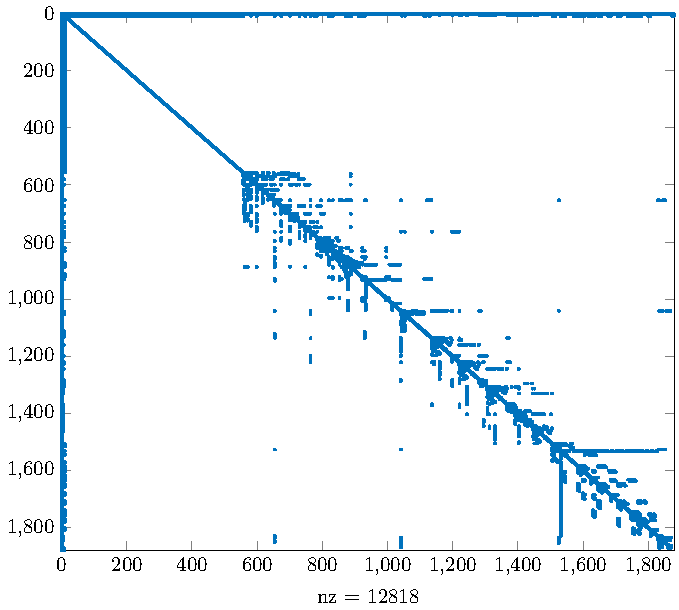
\includegraphics[scale=0.8]{../src/figure/rajat12.pdf}
\caption{Sparsity representation of the \texttt{rajat12} matrix.}
\label{fig:rajat12}
\end{figure}
Figure~\ref{fig:rajat12} shows the \texttt{rajat12} circuit matrix. This matrix is real and the matlab routine \texttt{issymmetric} finds it to be not symmetric. From a complex point of view it can thus be considered non-hermitian. However a closer look at Figure~\ref{fig:rajat12} reveals that the matrix is very close to being symmetric. In a first series of experiments the iterative GMRES method is used. The level of the incomplete LU-factorization, which is used for preconditioning is varied from between zero and one. Furthermore the amount of available vectors is increased successively from zero to one hundred. \\
Results for the time measurements are shown in Figure~\ref{fig:iluRajatCompTime}. Computations where run on a ThinkPad equipped with \texttt{8 GB} of ram and an i7-4800mq processor. The data shows a significant increase in computation time, for higher numbers of available vectors, with a zero level of fill. The same observation does not hold with a level of fill of one, here computations oscillate around an expected value of approximately two seconds. \\
Figure~\ref{fig:rajatConvergence} shows convergence of the residuals. Here it is important to note, that sufficient accuracy is reached using 10 Vectors within $\approx 230$ iterations for ILU level zero. It takes $\approx 20$ when the level of fill is set to one, due to improved conditioning of the problem. Curiously the decrease in iterations does not lead to on overall reduction of computation time. Probably in this case single iterations are much faster with zero level of fill, which would account for the timing difference. An overall increase of computation time can be observed for more vectors with in the zero level of fill setting. This is probably due to the fact that the overhead caused by the additional vectors becomes significant only when the amount of total iterations is large. Interestingly, when more vectors are used fewer iterations are required until convergence is reached. Large amounts of vectors are probably beneficial in settings, where larger matrices are used.
Memory requirements are shown in table~\ref{tab:RajatMemoryGMRES}. From the data it can be concluded that the higher ilu level does is neither 
advantageous in terms of memory consumption or computing time when the relatively small circuit matrix is considered. \\
Figure~\ref{fig:rajatSpectra}, shows the initial and preconditioned spectra. The normalizing effect of both preconditioners is clearly visible. Following the rule of thumb\footnote{Numerical linear algebra, Trefethen, Bau, page 314}: \\
\textquotedblleft A preconditioner $M$ is good if $M^{-1}$A is not too far from normal and its eigenvalues are clustered.\textquotedblright \\
Both preconditioners work but the higher level of fill gives more clustering, therefore it is better in this case.
The direct method implemented in the \texttt{mumps} requires \texttt{5.08 MB}  of ram and finishes within $0.004035s = 4.035*10^{-3}s$. It is thus faster then any iterative scheme tried above, with more then acceptable memory consumption. Storing some data on the hard drive using the \texttt{--ooc} option increases the computation time to $0.007442s$. In this cases this is clearly not necessary, as the memory needed is available on almost any modern computer.

\begin{figure}
\centering
% This file was created by matlab2tikz.
% Minimal pgfplots version: 1.3
%
%The latest updates can be retrieved from
%  http://www.mathworks.com/matlabcentral/fileexchange/22022-matlab2tikz
%where you can also make suggestions and rate matlab2tikz.
%
\documentclass[tikz]{standalone}
\usepackage{pgfplots}
\usepackage{grffile}
\pgfplotsset{compat=newest}
\usetikzlibrary{plotmarks}
\usepackage{amsmath}

\begin{document}
\definecolor{mycolor1}{rgb}{0.00000,0.44700,0.74100}%
%
\begin{tikzpicture}

\begin{axis}[%
width=1.5in,
height=1.5in,
at={(1.658854in,0.483542in)},
scale only axis,
xmin=0,
xmax=100,
xlabel={vectors},
ymin=0.016,
ymax=0.034,
ylabel={time [s]}
]
\addplot [color=mycolor1,solid,forget plot]
  table[row sep=crcr]{%
10	0.018125\\
11	0.022677\\
12	0.019412\\
13	0.020491\\
14	0.020396\\
15	0.019024\\
16	0.018773\\
17	0.017667\\
18	0.018628\\
19	0.017929\\
20	0.018139\\
21	0.018121\\
22	0.017523\\
23	0.019255\\
24	0.018598\\
25	0.018323\\
26	0.018326\\
27	0.018363\\
28	0.018373\\
29	0.01925\\
30	0.018653\\
31	0.01873\\
32	0.019364\\
33	0.019391\\
34	0.019466\\
35	0.019565\\
36	0.019688\\
37	0.019458\\
38	0.019964\\
39	0.020066\\
40	0.020697\\
41	0.021627\\
42	0.021546\\
43	0.020978\\
44	0.021024\\
45	0.021487\\
46	0.021248\\
47	0.021167\\
48	0.021313\\
49	0.021178\\
50	0.020938\\
51	0.021249\\
52	0.021826\\
53	0.022879\\
54	0.022944\\
55	0.023355\\
56	0.024061\\
57	0.024749\\
58	0.026311\\
59	0.025305\\
60	0.026383\\
61	0.026179\\
62	0.026303\\
63	0.027102\\
64	0.027013\\
65	0.025844\\
66	0.02657\\
67	0.026707\\
68	0.026278\\
69	0.025464\\
70	0.026814\\
71	0.025882\\
72	0.026522\\
73	0.025867\\
74	0.026382\\
75	0.026203\\
76	0.026442\\
77	0.026184\\
78	0.027455\\
79	0.027266\\
80	0.026837\\
81	0.028027\\
82	0.027961\\
83	0.027959\\
84	0.0292\\
85	0.028966\\
86	0.028973\\
87	0.029637\\
88	0.029366\\
89	0.030741\\
90	0.033256\\
91	0.030473\\
92	0.03094\\
93	0.032107\\
94	0.032836\\
95	0.032143\\
96	0.031817\\
97	0.032091\\
98	0.032285\\
99	0.033414\\
100	0.032784\\
};
\end{axis}

\begin{axis}[%
width=1.5in,
height=1.5in,
at={(4in,0.483542in)},
scale only axis,
xmin=0,
xmax=100,
xlabel={vectors},
ymin=1.6,
ymax=2.4,
ylabel={time [s]}
]
\addplot [color=mycolor1,solid,forget plot]
  table[row sep=crcr]{%
10	1.74676\\
11	1.71041\\
12	1.70631\\
13	1.70142\\
14	1.75954\\
15	1.84593\\
16	1.6833\\
17	1.70468\\
18	1.82023\\
19	1.76165\\
20	1.88569\\
21	1.77032\\
22	1.96255\\
23	1.74319\\
24	1.75664\\
25	2.108\\
26	1.82673\\
27	1.77709\\
28	1.70632\\
29	1.95466\\
30	1.76682\\
31	1.74808\\
32	1.75602\\
33	1.71269\\
34	1.7341\\
35	1.93888\\
36	1.75801\\
37	1.82413\\
38	1.83235\\
39	1.69602\\
40	1.72439\\
41	1.76215\\
42	1.72729\\
43	1.739\\
44	1.69348\\
45	1.84948\\
46	1.69432\\
47	1.71769\\
48	1.89903\\
49	1.77071\\
50	1.99037\\
51	1.67983\\
52	1.83828\\
53	1.92141\\
54	2.01674\\
55	1.80825\\
56	1.79346\\
57	1.86234\\
58	1.76435\\
59	1.74363\\
60	1.70756\\
61	1.71482\\
62	1.87778\\
63	1.69935\\
64	1.78105\\
65	1.7007\\
66	2.11195\\
67	1.7423\\
68	1.98093\\
69	1.84952\\
70	1.71318\\
71	2.0918\\
72	2.2592\\
73	2.24579\\
74	2.11869\\
75	2.21775\\
76	1.97425\\
77	2.35217\\
78	1.74441\\
79	1.71436\\
80	1.71036\\
81	2.08705\\
82	1.68541\\
83	1.76413\\
84	1.69961\\
85	1.69041\\
86	1.68632\\
87	1.68961\\
88	1.68019\\
89	1.67906\\
90	1.68073\\
91	1.68\\
92	1.69037\\
93	1.69836\\
94	1.6879\\
95	1.86636\\
96	1.7987\\
97	1.7434\\
98	1.79029\\
99	1.82523\\
100	1.72024\\
};
\end{axis}
\end{tikzpicture}%
\end{document}
\caption{CPU-Time of running \texttt{./ilu --method gmres --file rajat12.mtx  --nvectors \$vectors --tolerance 1.e-10} with \texttt{--ilu-level 0}(left) and \texttt{--ilu-level 1}(right) the value of the \texttt{\$vectors} variable is shown on the x axis.}
\label{fig:iluRajatCompTime}
\end{figure} 
\begin{figure}
\centering
% This file was created by matlab2tikz.
% Minimal pgfplots version: 1.3
%
%The latest updates can be retrieved from
%  http://www.mathworks.com/matlabcentral/fileexchange/22022-matlab2tikz
%where you can also make suggestions and rate matlab2tikz.
%
\documentclass[tikz]{standalone}
\usepackage{pgfplots}
\usepackage{grffile}
\pgfplotsset{compat=newest}
\usetikzlibrary{plotmarks}
\usepackage{amsmath}

\begin{document}
\definecolor{mycolor1}{rgb}{0.00000,0.44700,0.74100}%
\definecolor{mycolor2}{rgb}{0.85000,0.32500,0.09800}%
\definecolor{mycolor3}{rgb}{0.92900,0.69400,0.12500}%
\definecolor{mycolor4}{rgb}{0.49400,0.18400,0.55600}%
\definecolor{mycolor5}{rgb}{0.46600,0.67400,0.18800}%
%
\begin{tikzpicture}

\begin{axis}[%
width=5in,
height=3in,
at={(0.880208in,0.485833in)},
scale only axis,
xmode=log,
xmin=1,
xmax=1000,
xminorticks=true,
ymode=log,
ymin=1e-10,
ymax=10000,
yminorticks=true,
legend style={legend cell align=left,align=left,draw=white!15!black}
]
\addplot [color=mycolor1,solid]
  table[row sep=crcr]{%
1	500.369\\
2	22.038\\
3	19.6888\\
4	15.3888\\
5	3.80827\\
6	3.47815\\
7	2.38605\\
8	1.67397\\
9	0.881279\\
10	0.764443\\
11	0.63658\\
12	0.63595\\
13	0.617115\\
14	0.561676\\
15	0.49268\\
16	0.441212\\
17	0.314882\\
18	0.3014\\
19	0.250091\\
20	0.20548\\
21	0.189347\\
22	0.188932\\
23	0.188922\\
24	0.165311\\
25	0.139327\\
26	0.119566\\
27	0.111493\\
28	0.104409\\
29	0.0956074\\
30	0.0818959\\
31	0.0746758\\
32	0.074504\\
33	0.0738679\\
34	0.0657146\\
35	0.0585845\\
36	0.0555147\\
37	0.0459553\\
38	0.0399038\\
39	0.038795\\
40	0.0352988\\
41	0.0280612\\
42	0.0280388\\
43	0.0280038\\
44	0.0229191\\
45	0.0223529\\
46	0.0217129\\
47	0.0196485\\
48	0.0192655\\
49	0.0163879\\
50	0.015491\\
51	0.0151046\\
52	0.0148836\\
53	0.0148294\\
54	0.0140856\\
55	0.0126093\\
56	0.0119374\\
57	0.0109909\\
58	0.0108273\\
59	0.0107408\\
60	0.00786344\\
61	0.0074886\\
62	0.00748795\\
63	0.00743965\\
64	0.00626089\\
65	0.00621341\\
66	0.00596183\\
67	0.00522652\\
68	0.00517355\\
69	0.00492205\\
70	0.00433876\\
71	0.00421775\\
72	0.00421633\\
73	0.00418939\\
74	0.00405748\\
75	0.00380341\\
76	0.0035799\\
77	0.00335351\\
78	0.00314137\\
79	0.00298536\\
80	0.00259294\\
81	0.00196418\\
82	0.00196293\\
83	0.00192117\\
84	0.0015099\\
85	0.00142025\\
86	0.00136509\\
87	0.00117798\\
88	0.00113713\\
89	0.0010902\\
90	0.00105662\\
91	0.00101922\\
92	0.00101528\\
93	0.00101238\\
94	0.00094254\\
95	0.000915138\\
96	0.000817576\\
97	0.00077624\\
98	0.000699672\\
99	0.00069922\\
100	0.000502859\\
101	0.000395298\\
102	0.000395094\\
103	0.00039069\\
104	0.000327492\\
105	0.000280976\\
106	0.000228794\\
107	0.000209661\\
108	0.000208141\\
109	0.000186724\\
110	0.000173392\\
111	0.0001627\\
112	0.000161835\\
113	0.000160896\\
114	0.000158127\\
115	0.000147882\\
116	0.000143068\\
117	0.000120373\\
118	0.000116713\\
119	0.000103079\\
120	8.80536e-05\\
121	7.24922e-05\\
122	7.24826e-05\\
123	7.05322e-05\\
124	6.62605e-05\\
125	5.13077e-05\\
126	4.37749e-05\\
127	4.3153e-05\\
128	3.71366e-05\\
129	3.56918e-05\\
130	3.44443e-05\\
131	3.33401e-05\\
132	3.33114e-05\\
133	3.33114e-05\\
134	3.22308e-05\\
135	3.09106e-05\\
136	2.94616e-05\\
137	2.63044e-05\\
138	2.42314e-05\\
139	2.10179e-05\\
140	1.97969e-05\\
141	1.41261e-05\\
142	1.41059e-05\\
143	1.20928e-05\\
144	9.707e-06\\
145	8.81524e-06\\
146	7.52536e-06\\
147	7.45899e-06\\
148	6.99572e-06\\
149	6.51222e-06\\
150	6.40995e-06\\
151	6.23656e-06\\
152	6.2344e-06\\
153	6.2106e-06\\
154	5.98066e-06\\
155	5.84211e-06\\
156	5.7219e-06\\
157	5.05238e-06\\
158	4.75099e-06\\
159	3.92556e-06\\
160	3.73283e-06\\
161	3.38453e-06\\
162	3.37949e-06\\
163	3.30204e-06\\
164	2.92418e-06\\
165	2.56884e-06\\
166	2.31386e-06\\
167	2.1542e-06\\
168	2.02591e-06\\
169	2.01431e-06\\
170	1.89075e-06\\
171	1.66982e-06\\
172	1.66969e-06\\
173	1.62946e-06\\
174	1.48291e-06\\
175	1.44125e-06\\
176	1.39392e-06\\
177	1.3457e-06\\
178	1.32349e-06\\
179	1.19676e-06\\
180	1.17721e-06\\
181	1.01229e-06\\
182	1.01007e-06\\
183	1.00896e-06\\
184	9.12563e-07\\
185	8.56499e-07\\
186	8.26235e-07\\
187	7.55695e-07\\
188	7.36479e-07\\
189	7.05934e-07\\
190	6.75887e-07\\
191	6.69514e-07\\
192	6.68901e-07\\
193	6.65051e-07\\
194	6.28447e-07\\
195	5.9542e-07\\
196	5.76106e-07\\
197	5.34408e-07\\
198	5.20654e-07\\
199	4.81141e-07\\
200	4.51509e-07\\
201	3.92349e-07\\
202	3.92214e-07\\
203	3.59065e-07\\
204	3.28527e-07\\
205	3.03682e-07\\
206	2.99775e-07\\
207	2.59004e-07\\
208	2.55535e-07\\
209	2.55182e-07\\
210	2.37036e-07\\
211	2.33896e-07\\
212	2.33864e-07\\
213	2.33286e-07\\
214	2.22686e-07\\
215	2.17212e-07\\
216	2.04802e-07\\
217	1.8963e-07\\
218	1.82018e-07\\
219	1.67664e-07\\
220	1.55414e-07\\
221	1.49292e-07\\
222	1.49091e-07\\
223	1.42232e-07\\
224	1.28799e-07\\
225	1.22304e-07\\
226	1.10614e-07\\
227	1.10423e-07\\
228	9.92083e-08\\
229	9.77978e-08\\
230	9.63762e-08\\
231	5.979e-08\\
232	5.92204e-08\\
233	5.60487e-08\\
234	5.26796e-08\\
235	4.27657e-08\\
};
\addlegendentry{GMRES(0,10)};

\addplot [color=mycolor2,solid]
  table[row sep=crcr]{%
1	500.369\\
2	22.038\\
3	19.6888\\
4	15.3888\\
5	3.80827\\
6	3.47815\\
7	2.38605\\
8	1.67397\\
9	0.881279\\
10	0.764443\\
11	0.63658\\
12	0.524831\\
13	0.374078\\
14	0.330155\\
15	0.227443\\
16	0.180574\\
17	0.158163\\
18	0.130202\\
19	0.1165\\
20	0.0909158\\
21	0.0735541\\
22	0.0631711\\
23	0.0545801\\
24	0.0453725\\
25	0.0405525\\
26	0.0351084\\
27	0.0269106\\
28	0.0240316\\
29	0.0218387\\
30	0.0180676\\
31	0.0167174\\
32	0.013394\\
33	0.0116374\\
34	0.0101062\\
35	0.00861708\\
36	0.0078851\\
37	0.00685004\\
38	0.00597064\\
39	0.00548146\\
40	0.00461292\\
41	0.00416415\\
42	0.00355456\\
43	0.00301608\\
44	0.00275413\\
45	0.00213296\\
46	0.00197839\\
47	0.00170531\\
48	0.00142577\\
49	0.00131094\\
50	0.00108817\\
51	0.000934799\\
52	0.000807608\\
53	0.000697967\\
54	0.000588392\\
55	0.000538466\\
56	0.00045428\\
57	0.000363634\\
58	0.000327435\\
59	0.000255393\\
60	0.000227886\\
61	0.000191218\\
62	0.000152948\\
63	0.000140119\\
64	0.000111837\\
65	9.73151e-05\\
66	8.68994e-05\\
67	6.57036e-05\\
68	5.63644e-05\\
69	4.88928e-05\\
70	3.38404e-05\\
71	2.98015e-05\\
72	2.43543e-05\\
73	2.24543e-05\\
74	1.8793e-05\\
75	1.45818e-05\\
76	1.36042e-05\\
77	1.19902e-05\\
78	1.02736e-05\\
79	9.29386e-06\\
80	8.15408e-06\\
81	6.66215e-06\\
82	5.79887e-06\\
83	5.07747e-06\\
84	4.11576e-06\\
85	3.71987e-06\\
86	2.98484e-06\\
87	2.55551e-06\\
88	2.18874e-06\\
89	1.7039e-06\\
90	1.56536e-06\\
91	1.1993e-06\\
92	9.61673e-07\\
93	8.67617e-07\\
94	6.508e-07\\
95	5.76919e-07\\
96	5.15324e-07\\
97	3.81373e-07\\
98	3.44414e-07\\
99	2.73879e-07\\
100	2.31043e-07\\
101	2.06626e-07\\
102	2.06348e-07\\
103	1.97756e-07\\
104	1.73224e-07\\
105	1.66221e-07\\
106	1.5552e-07\\
107	1.3326e-07\\
108	1.30994e-07\\
109	1.00624e-07\\
110	9.61358e-08\\
111	9.40316e-08\\
112	8.30843e-08\\
113	7.45508e-08\\
114	5.42891e-08\\
115	4.82348e-08\\
};
\addlegendentry{GMRES(0,100)};

\addplot [color=mycolor3,solid]
  table[row sep=crcr]{%
1	196.828\\
2	45.7866\\
3	20.2302\\
4	3.9265\\
5	1.79062\\
6	0.227687\\
7	0.0378213\\
8	0.00493087\\
9	0.000510816\\
10	8.14384e-05\\
11	8.31152e-06\\
12	4.00801e-06\\
13	3.97243e-06\\
14	8.00432e-07\\
15	1.08139e-07\\
16	2.1581e-08\\
17	3.27388e-09\\
};
\addlegendentry{GMRES(1,10)};

\addplot [color=mycolor4,solid]
  table[row sep=crcr]{%
1	196.828\\
2	45.7866\\
3	20.2302\\
4	3.9265\\
5	1.79062\\
6	0.227687\\
7	0.0378213\\
8	0.00493087\\
9	0.000510816\\
10	8.14384e-05\\
11	8.31152e-06\\
12	9.73394e-07\\
13	9.01129e-08\\
14	9.79281e-09\\
};
\addlegendentry{GMRES(1,100)};

\addplot [color=mycolor5,solid]
  table[row sep=crcr]{%
1	4.99997\\
2	2241.27\\
3	90.4235\\
4	98.9266\\
5	4.70531\\
6	6.43126\\
7	4.43646\\
8	19.6816\\
9	14.7451\\
10	24.1273\\
11	15.8001\\
12	22.0078\\
13	17.1668\\
14	30.9871\\
15	20.3704\\
16	1.37373\\
17	1.11559\\
18	1.42346\\
19	1.09643\\
20	0.555871\\
21	0.454585\\
22	0.312441\\
23	0.272605\\
24	0.219478\\
25	0.19395\\
26	0.179866\\
27	0.143543\\
28	0.102629\\
29	0.0985018\\
30	0.100547\\
31	0.0968439\\
32	0.0539646\\
33	0.0423077\\
34	0.0681046\\
35	0.053851\\
36	0.023508\\
37	0.0228025\\
38	0.0227116\\
39	0.0220803\\
40	0.0165206\\
41	0.0145579\\
42	0.0139976\\
43	0.00979606\\
44	1.1291\\
45	0.168512\\
46	0.00725263\\
47	0.00682896\\
48	0.00529193\\
49	0.00443099\\
50	0.00449544\\
51	0.00428657\\
52	0.00355027\\
53	0.00340881\\
54	0.00339726\\
55	0.00329528\\
56	0.00227781\\
57	0.00213611\\
58	0.00213392\\
59	0.00190863\\
60	0.00169325\\
61	0.00165801\\
62	0.00166881\\
63	0.00163417\\
64	0.00160619\\
65	0.00124193\\
66	0.00185899\\
67	0.00102353\\
68	0.00310226\\
69	0.00268472\\
70	0.000550625\\
71	0.000544212\\
72	0.000615112\\
73	0.000607466\\
74	0.000604596\\
75	0.000588014\\
76	0.00109391\\
77	0.000584477\\
78	0.000384052\\
79	0.000371663\\
80	0.000372848\\
81	0.000368739\\
82	0.000353667\\
83	0.000305541\\
84	0.0152227\\
85	0.000104184\\
86	0.000336358\\
87	0.000296139\\
88	0.000640048\\
89	0.000247878\\
90	0.000162005\\
91	0.000159603\\
92	0.000164656\\
93	0.000162304\\
94	0.000101635\\
95	9.9757e-05\\
96	9.86661e-05\\
97	9.75881e-05\\
98	0.000111399\\
99	0.000106612\\
100	3.77926e-05\\
101	3.57317e-05\\
102	3.44248e-05\\
103	3.32829e-05\\
104	5.96917e-05\\
105	3.31664e-05\\
106	2.66868e-05\\
107	1.9512e-05\\
108	1.98518e-05\\
109	1.96548e-05\\
110	2.18441e-05\\
111	2.02387e-05\\
112	5.84851e-06\\
113	5.78875e-06\\
114	8.20267e-06\\
115	2.48269e-06\\
116	7.20187e-06\\
117	9.90175e-07\\
118	1.36989e-06\\
119	1.23936e-06\\
120	6.07703e-07\\
121	5.35322e-07\\
122	3.80122e-07\\
123	3.2915e-07\\
124	2.39091e-07\\
125	2.34073e-07\\
126	1.50329e-07\\
127	1.46658e-07\\
128	1.23153e-07\\
129	1.20607e-07\\
130	1.05302e-07\\
131	9.74903e-08\\
132	7.79068e-08\\
133	5.19795e-08\\
134	4.39897e-08\\
135	4.1041e-08\\
136	8.22946e-08\\
137	4.62362e-08\\
138	1.58049e-08\\
139	1.151e-08\\
140	1.31686e-08\\
141	1.1917e-08\\
142	1.96609e-08\\
143	1.44159e-08\\
144	9.31626e-09\\
145	9.10656e-09\\
146	9.31035e-09\\
147	9.15905e-09\\
148	9.25633e-09\\
149	8.92102e-09\\
150	8.53318e-09\\
151	8.2338e-09\\
152	7.96436e-09\\
153	7.85852e-09\\
154	5.58026e-08\\
155	3.80641e-08\\
156	2.08562e-09\\
157	2.01075e-09\\
158	1.14121e-09\\
159	1.05817e-09\\
160	9.97801e-10\\
161	8.42218e-10\\
162	7.36821e-10\\
163	7.12316e-10\\
164	8.53316e-10\\
165	6.27853e-10\\
166	6.63774e-10\\
167	6.52578e-10\\
168	6.51442e-10\\
169	6.4091e-10\\
170	9.82494e-10\\
171	9.22931e-10\\
172	5.89147e-10\\
173	4.94543e-10\\
};
\addlegendentry{BicStab(0,10)};

\end{axis}
\end{tikzpicture}%
\end{document}
\caption{GMRES convergence with the rajat12 matrix with ILu level 0 and 1.}
\label{fig:rajatConvergence}
\end{figure}
\begin{table}
\centering
\begin{tabular}{|c|c|c|c|} \hline
  \#vectors & ilu level of fill & memory & relative error \\
   10 & 1 & \texttt{155.9 MB} & $1.13517 \cdot 10^{-10}$ \\
   100 & 1 & \texttt{157.3 MB}& $2.4985  \cdot 10^{-10}$ \\
   10 &  0 & \texttt{3.1 MB}  & $8.23038 \cdot 10^{-08}$ \\
   100 & 0 & \texttt{4.35 MB} & $5.64681 \cdot 10^{-08}$ \\ \hline
\end{tabular}
\caption{Memory requirements of GMRES when run on the rajat12 matrix. }
\label{tab:RajatMemoryGMRES}
\begin{tabular}{|c|c|c|c|c|} \hline
  \#vectors & ilu level of fill  & memory & CPU time & relative error \\
   10  & 1  & \texttt{155.8 MB}    & 1.67045 s & $6.55193 \cdot 10^{-11}$ \\
   100 & 1  & \texttt{155.823 MB} & 1.94236 s & $6.55193 \cdot 10^{-11}$  \\
   10  & 0  & \texttt{3.042 MB}   & 0.00815 s & $2.09145 \cdot 10^{-09}$  \\
   100 & 0  & \texttt{3.042 MB}   & 0.01006 s & $2.09145 \cdot 10^{-09}$  \\ \hline
\end{tabular}
\caption{Memory and time requirements of bicgstab when run on the rajat12 matrix. }
\label{tab:RajatMemoryBicgstab}
\end{table}
\begin{figure}
\centering
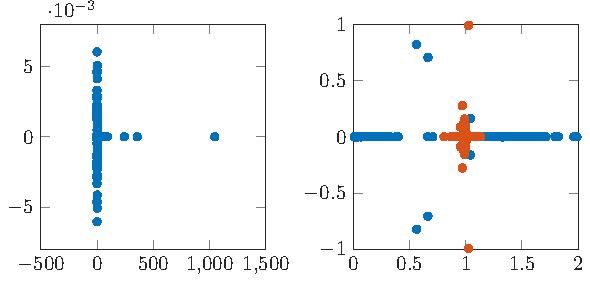
\includegraphics[scale=1]{../src/figure/spectraRajat12.pdf}
%% This file was created by matlab2tikz v0.4.7 running on MATLAB 8.5.
% Copyright (c) 2008--2014, Nico Schlömer <nico.schloemer@gmail.com>
% All rights reserved.
% Minimal pgfplots version: 1.3
% 
% The latest updates can be retrieved from
%   http://www.mathworks.com/matlabcentral/fileexchange/22022-matlab2tikz
% where you can also make suggestions and rate matlab2tikz.
% 
\documentclass[tikz]{standalone}
\usepackage{pgfplots}
\usepackage{grffile}
\pgfplotsset{compat=newest}
\usetikzlibrary{plotmarks}
\usepackage{amsmath}

\begin{document}
%
% defining custom colors
\definecolor{mycolor1}{rgb}{0.00000,0.44700,0.74100}%
\definecolor{mycolor2}{rgb}{0.85000,0.32500,0.09800}%
%
\begin{tikzpicture}

\begin{axis}[%
width=1.5in,
height=1.5in,
scale only axis,
separate axis lines,
every outer x axis line/.append style={white!15!black},
every x tick label/.append style={font=\color{white!15!black}},
xmin=-500,
xmax=1500,
every outer y axis line/.append style={white!15!black},
every y tick label/.append style={font=\color{white!15!black}},
ymin=-0.008,
ymax=0.008,
name=plot1
]
\addplot [color=mycolor1,only marks,mark=*,mark options={solid},forget plot]
  table[row sep=crcr]{1047.29815201591	0\\
357.877584204619	0\\
242.897308345831	0\\
92.2503566291336	0\\
78.6578597480995	0\\
50.472748737374	0\\
41.4322443693913	0\\
38.1713318245436	0\\
27.8950354612715	0\\
23.8259447172687	0\\
18.0045003280556	0\\
12.9945563119527	0\\
20.9038827402654	0\\
20.8978410930135	0\\
20.8976061965757	0\\
20.8961316850475	0\\
20.8958477048557	0\\
20.8953940404802	0\\
20.8955585715939	0\\
20.8955156760486	0\\
11.7522816126353	0\\
8.69389589518882	0\\
8.58425951078492	0\\
8.45466084906094	0\\
8.03343287264466	0\\
7.81359167200324	0\\
7.79943312064493	0\\
7.79104258326008	0\\
7.78451147724325	0\\
7.78081447163391	0\\
7.78146093598581	0\\
7.73057806320756	0\\
7.70508728558509	0\\
7.67271023029415	0\\
7.66864684933175	0\\
7.66188808348286	0\\
7.65836287939247	0\\
7.65426751514009	0\\
7.38838442630385	0\\
7.38939801011705	0\\
7.25443249875315	0\\
7.25658058047769	0\\
7.08590596725249	0\\
7.0665609266398	0\\
6.97885221080755	0\\
6.90350558270556	0\\
6.8430274042077	0\\
6.6483424406183	0\\
6.45155053279957	0\\
6.38383715723975	0\\
6.39551304848687	0\\
6.19690669290933	0\\
5.56241933481049	0\\
6.22518878202494	0\\
6.22509277817114	0\\
6.22509291183186	0\\
4.80572871494284	0\\
4.78489878193107	0\\
4.4837501026667	0\\
4.48429533513369	0\\
4.53471066091145	0\\
4.53471071483334	0\\
4.09176202923526	0\\
3.99030194464551	0\\
3.95428003986651	0\\
3.93197603285984	0\\
3.93100140205801	0\\
3.91363413089115	0\\
3.88671190509238	0\\
3.87724734578243	0\\
3.62240813759465	0.000592627946964726\\
3.62240813759465	-0.000592627946964726\\
3.62128569899305	0\\
3.73646405362475	0\\
3.7380622197238	0\\
3.73812275459653	0\\
3.73811702322689	0\\
3.73811703398977	0\\
3.28844118473144	0\\
3.3230259984888	0\\
3.31753634609856	0\\
3.30792225333134	0\\
3.30807015741629	0\\
3.33385796239175	0\\
3.33643121864808	0.000550198536066991\\
3.33643121864808	-0.000550198536066991\\
3.33644560473943	0.000551505576573188\\
3.33644560473943	-0.000551505576573188\\
3.18799618325145	0\\
3.17231794258786	0\\
3.17665039637194	0\\
3.17578919200791	0\\
3.11394358864351	0\\
2.97987322311844	0\\
2.83814038423009	0\\
2.83840204013647	0\\
2.76951356371019	0\\
2.74414064953716	0\\
2.70659628274085	0\\
2.70230384201893	0\\
2.69148253886648	0\\
2.69733655975391	0\\
2.69615387658857	0\\
2.62882339844446	0\\
-0.973197661254783	0\\
-0.96488326551753	0\\
-0.961423073460401	0\\
-0.940550098136274	0\\
-0.932188923334964	0\\
-0.930857249059903	0\\
2.38940056494511	0\\
2.3924245611743	0\\
2.42636212040177	0\\
2.62356911865025	0\\
2.62356911865024	0\\
2.62356911865022	0\\
2.41800097396139	0\\
2.41799944930682	0\\
2.41799919456066	9.48489589977536e-08\\
2.41799919456066	-9.48489589977536e-08\\
2.41799925957563	6.4790279539192e-08\\
2.41799925957563	-6.4790279539192e-08\\
2.53072958081398	0\\
2.51881649758084	0\\
2.48507778497835	0\\
2.4851816285265	0\\
2.48524380533502	0\\
2.51345690394745	0\\
2.51343186518185	0\\
2.51348213827995	0\\
2.57137112846056	0\\
2.55467386922797	0\\
2.58699114673978	0\\
2.58698820416011	0\\
2.58698820416009	0\\
2.56287331756127	0\\
2.57522228319018	1.33060955831366e-07\\
2.57522228319018	-1.33060955831366e-07\\
2.57522241457178	1.13577483991455e-07\\
2.57522241457178	-1.13577483991455e-07\\
2.57522290892544	0\\
2.57522303359597	0\\
2.5575323182388	0\\
2.56499307035301	0\\
2.56484509791272	0\\
2.56517144435785	0\\
2.56482401597514	0\\
2.56489323272368	0\\
2.48514830334495	0\\
2.48514830334496	0\\
2.48543632991154	0\\
2.48543632991154	0\\
2.48543632991156	0\\
2.50177830505643	0\\
2.55792295917424	0\\
2.55792409523134	0\\
2.55792407784614	3.64138982833187e-09\\
2.55792407784614	-3.64138982833187e-09\\
2.5579240808062	2.7987503921698e-09\\
2.5579240808062	-2.7987503921698e-09\\
2.55812079990539	0\\
2.55812206852104	0\\
2.55812206852105	0\\
2.55812206852104	0\\
2.50177830505645	0\\
2.50177830505642	1.72531658603426e-15\\
2.50177830505642	-1.72531658603426e-15\\
2.50177830505641	0\\
2.27925043404529	0\\
2.5869882041601	0\\
2.10332401220952	0\\
2.20723014756607	0\\
2.30180234646099	0\\
2.31265403638585	0\\
2.14703519301086	0\\
2.38945025880495	0\\
2.38934576727631	0\\
2.3925789209991	0\\
2.39224955564216	0\\
2.40023188134977	0\\
2.43990369149222	0\\
2.15938905622096	0\\
2.1582087649489	0\\
2.15836851438485	5.18359756313865e-05\\
2.15836851438485	-5.18359756313865e-05\\
2.15839972928559	2.97179636841567e-05\\
2.15839972928559	-2.97179636841567e-05\\
2.15840651560102	0\\
2.43989804365116	0\\
2.43989804365116	0\\
2.39868485326026	0\\
2.48514830334497	0\\
2.43989804365116	0\\
2.39868479583991	0\\
2.3094705467608	0\\
2.23982167008845	0\\
2.23982167008847	0\\
2.23982167008847	0\\
2.30946686886557	0\\
2.39868479583991	0\\
2.39868479583989	0\\
2.23581469665507	0\\
2.23581469665504	0\\
2.23581469665505	0\\
2.23581469665506	0\\
2.30936769494357	0\\
2.30936769494359	0\\
2.30936769494357	3.53183565073564e-15\\
2.30936769494357	-3.53183565073564e-15\\
2.30936769494358	0\\
2.30936769494358	7.50940934905391e-16\\
2.30936769494358	-7.50940934905391e-16\\
2.30936769494358	0\\
2.23982167008847	0\\
2.23581469665505	0\\
2.23581469665506	0\\
2.58698820416007	0\\
2.5869882041601	0\\
2.58698820416008	0\\
1.96838354303575	0\\
1.97402038187108	0\\
2.03396482025407	0\\
2.40023188134976	0\\
2.07676332416878	0\\
2.40023188134979	0\\
2.02147579149773	0\\
2.00490422758448	0\\
2.43989804365113	0\\
2.01004266518226	0\\
2.00986865994567	0\\
2.00963825738989	0\\
2.001899	0\\
2.00966774431608	0\\
2.07437821900955	0\\
2.07440930850519	0\\
2.01674460699738	0\\
2.07439379756181	1.99237810126539e-06\\
2.07439379756181	-1.99237810126539e-06\\
2.0743952091705	1.13869029913488e-06\\
2.0743952091705	-1.13869029913488e-06\\
2.01524916462385	0\\
2.01562045082657	8.20126127899655e-05\\
2.01562045082657	-8.20126127899655e-05\\
2.01566885927392	0\\
2.01559122095197	4.18595106137468e-05\\
2.01559122095197	-4.18595106137468e-05\\
2.07439385843246	0\\
2.01562044249151	0\\
2.48514830334496	0\\
2.48514830334494	0\\
2.48543632991151	0\\
2.48543632991155	0\\
2.48543632991153	0\\
2.39868479583991	0\\
2.00199100000002	0\\
2.001991	0\\
2.001991	0\\
2.00199099999999	0\\
2.55812206852102	0\\
2.55812206852107	0\\
1.83039090393522	0\\
1.80818248226548	0\\
2.01722799999999	0\\
1.75767129823596	0\\
1.79607613684557	0\\
1.79577317754079	0\\
1.79949162286513	0\\
1.77637709882398	0\\
1.78104583517032	0\\
1.78466525213699	0\\
1.79952695756303	0\\
1.79953222940716	0\\
1.78159246320547	0\\
1.78364390942789	0\\
1.78259405173869	0\\
1.78253134979333	0\\
2.43989804365116	0\\
2.50177830505644	1.69831466010162e-15\\
2.50177830505644	-1.69831466010162e-15\\
2.43989804365116	0\\
2.3986847958399	0\\
2.23982167008848	0\\
2.485148303345	0\\
2.23982167008847	0\\
2.23982167008847	0\\
2.48514830334497	0\\
2.30936769494357	0\\
2.55812206852105	0\\
2.3986847958399	0\\
1.71899997188283	0\\
2.50177830505641	0\\
2.50177830505644	0\\
1.73678388318871	0\\
1.70960941708888	0\\
1.69170287919692	0\\
1.71353081550794	0\\
1.71361454213427	0\\
-0.0540738017680939	0\\
1.70247382148826	0\\
1.64632794564593	0\\
1.71360196665082	6.09138869960357e-06\\
1.71360196665082	-6.09138869960357e-06\\
1.71360324036873	0\\
1.71359944693089	0\\
1.67715895198078	0\\
1.70245774119505	0\\
1.70251107900092	0\\
1.64781786172003	0\\
1.66769813113443	0\\
1.57159271271709	0\\
1.64484713481815	0\\
1.67471899662199	0\\
1.67473924357999	0\\
1.67473616140033	6.67775928094184e-07\\
1.67473616140033	-6.67775928094184e-07\\
1.67473535661913	3.70795199290703e-07\\
1.67473535661913	-3.70795199290703e-07\\
2.001991	0\\
1.68344330850776	0\\
2.001991	0\\
2.48543632991152	0\\
2.48543632991153	0\\
2.48543632991152	0\\
2.48514830334494	0\\
2.00199099999999	0\\
2.23581469665503	0\\
2.23581469665504	0\\
2.23581469665505	0\\
1.68344595634885	0\\
2.48514830334496	0\\
2.23982167008847	0\\
2.23982167008848	0\\
2.48543632991154	0\\
1.68344595634885	0\\
2.48514830334496	0\\
1.53699346082983	0\\
1.53462691106207	0\\
2.23581469665503	0\\
1.56188793147894	0\\
1.5618922000946	0\\
2.23982167008847	0\\
2.23982167008845	0\\
1.56188793147895	0\\
1.56188793147894	0\\
2.48514830334496	0\\
2.48543632991154	0\\
2.48543632991154	0\\
-0.0303729264020917	0\\
2.48514830334496	0\\
2.23581469665505	0\\
2.23982167008847	0\\
2.48543632991154	0\\
-0.0121691439268874	0\\
1.68344595634885	0\\
2.23581469665504	0\\
1.68344595634886	0\\
2.48514830334498	0\\
2.23581469665504	0\\
2.23982167008847	0\\
1.52282998402486	0\\
0.00151484438837924	0\\
0.00216377676307339	0\\
0.00216357913375383	0\\
0.00216312600570455	0\\
1.68344595634884	0\\
1.68344595634884	0\\
1.56188793147897	0\\
1.12327207382871	0\\
1.11799573508081	0\\
1.1163264181689	0\\
1.35290780504303	0\\
1.32060274541632	0\\
1.31480274974356	0\\
1.30945400158051	0\\
1.30709107729984	0.000510190738343425\\
1.30709107729984	-0.000510190738343425\\
1.37738835903844	0\\
1.30508540950403	0.00081919915192551\\
1.30508540950403	-0.00081919915192551\\
1.29885757056358	0\\
1.29004637608716	0.00506937807492582\\
1.29004637608716	-0.00506937807492582\\
1.29424207930395	0\\
1.27084986216149	0\\
1.29189832268228	0.00113788432126869\\
1.29189832268228	-0.00113788432126869\\
1.28316037573784	0.00413597293444821\\
1.28316037573784	-0.00413597293444821\\
1.28783756569988	0.000279737517306064\\
1.28783756569988	-0.000279737517306064\\
1.28429621406536	0.00112408090738493\\
1.28429621406536	-0.00112408090738493\\
1.27750371402873	0\\
1.28073034609523	0.00105191154975816\\
1.28073034609523	-0.00105191154975816\\
1.27937511036244	0.000877509529449312\\
1.27937511036244	-0.000877509529449312\\
1.17409215561352	0\\
1.36588835845446	0\\
1.27975471410879	0\\
1.17457131980386	0\\
1.36773607562829	0\\
1.17475959135781	0\\
1.36867072249787	4.41838135447583e-05\\
1.36867072249787	-4.41838135447583e-05\\
1.36829713662737	0.000119639521162384\\
1.36829713662737	-0.000119639521162384\\
1.2538599799777	0\\
1.25919940049345	0\\
1.36810992640469	0.00016828203797627\\
1.36810992640469	-0.00016828203797627\\
1.17497571287379	0\\
1.17442458206841	0\\
1.17442459550419	0\\
1.25322182253098	0\\
1.25875625080191	0\\
1.2587522804392	0\\
1.25874346711394	0\\
1.17442459733415	0\\
1.17497573842527	0\\
1.1749757381822	0\\
1.25873966794633	0\\
1.25874987470779	0\\
1.25873936101608	0\\
1.26424414922297	0\\
1.254141	0\\
1.29591911681129	0\\
1.56188793147894	0\\
1.46971574982736	0\\
1.45727949833402	0\\
1.09300996427239	0\\
1.08992465256625	0\\
1.08228212864556	0\\
1.07454171436372	0\\
0.101165247025547	0\\
0.0878262252211071	0\\
0.0853135257929892	0\\
0.0721147777647796	0.00225937121243828\\
0.0721147777647796	-0.00225937121243828\\
0.0714470286231587	0\\
0.00279967344210845	0\\
0.0660808408412388	0.00604197337708828\\
0.0660808408412388	-0.00604197337708828\\
0.0683317585510536	0\\
0.0662331892200689	0\\
0.0648416858950716	0\\
0.0619008065979152	0.00468073794363514\\
0.0619008065979152	-0.00468073794363514\\
0.00438641510961533	0\\
0.00324143119823489	0\\
0.00324027534128884	0\\
0.00324069675768951	0\\
0.0593322171253518	0.00331683288639802\\
0.0593322171253518	-0.00331683288639802\\
0.0616371555260422	0\\
0.0612106003827127	0\\
0.0564172102841073	0.00459481708538226\\
0.0564172102841073	-0.00459481708538226\\
0.00539916990551391	0\\
0.00540672190209602	0\\
0.0503427863905283	0.0020349460763053\\
0.0503427863905283	-0.0020349460763053\\
0.00613835537574439	0\\
0.0550389393445926	0\\
0.0543092218813553	0\\
0.0495069471563079	0\\
0.00620957168819345	0\\
0.00630157281124272	0\\
0.00627397133070505	0\\
0.0534428479942885	0\\
0.0530491270483553	0\\
0.00624735792021986	0\\
1.56188793147896	0\\
1.07472338505292	0\\
1.39662684533634	0\\
1.06464956321414	0\\
1.06425985487024	0\\
1.39581538077026	0\\
0.113112207208825	0\\
0.110226892756942	0\\
0.102469947140756	0\\
0.103599125912632	0\\
0.1069752679669	0\\
0.00815918178466247	0\\
0.105827366153688	0\\
0.105866209116103	0\\
0.0480722508430099	0\\
0.105855704120627	0\\
0.105861718728751	0\\
0.0473319171168267	0\\
0.0441180695613959	0\\
0.0461916938987973	0\\
0.0452368511208848	0\\
0.0433753639547137	0\\
0.0402783037721536	0\\
0.0414484977441486	0\\
0.0421741737283128	0\\
0.0428237207553945	0\\
0.00882144859094285	0\\
0.0118263325556242	0.00205400422645578\\
0.0118263325556242	-0.00205400422645578\\
0.0379210349381931	0\\
0.0367886225627002	0\\
0.0131083613950181	0.0022924104616651\\
0.0131083613950181	-0.0022924104616651\\
0.0121487861461946	0.00217766314292044\\
0.0121487861461946	-0.00217766314292044\\
0.00933612478646947	0\\
0.00937382025761187	0\\
0.00947642452834763	0\\
0.00961120592216643	0\\
0.0357425838997141	0\\
0.0352220537607784	0\\
0.034608761988822	0\\
0.0341114288157059	0\\
0.0337590510038848	0\\
0.0335425142610698	0\\
0.0340243439999901	0\\
0.0326736282436509	0\\
0.0332422770486953	0\\
0.0320966060867822	0\\
0.0312184106141097	0\\
0.0315612120327166	0\\
0.0131755745623868	0\\
0.0292288694429035	0\\
0.0285805229198341	0\\
0.0138894890012035	0.000173675586650346\\
0.0138894890012035	-0.000173675586650346\\
0.0136624047406229	0\\
0.0283931335004348	0\\
0.0148501543675317	0\\
0.0115390159788551	0\\
0.0125228884088101	0\\
0.0306438389097043	0\\
0.0125675278261072	0\\
0.0150592027277706	0\\
0.0113161432855532	0\\
0.0259754991706454	0\\
0.0266888005095972	0\\
0.0264518747966583	0\\
0.0271700810748023	0\\
0.0274318016337753	0\\
0.0261798369088573	0\\
0.0303315642520237	0\\
0.0105586198937823	0\\
0.0305189811645744	0\\
0.011160282459259	0\\
0.0307088265158133	0\\
0.0197703407007433	0\\
0.010980872147251	0\\
0.0301064471455244	0\\
0.023902610789077	0\\
0.0162107455500884	0\\
0.0186584657934122	0.000479793267178386\\
0.0186584657934122	-0.000479793267178386\\
0.0195625064874657	0\\
0.016419763470792	0\\
0.0232680050864907	0\\
0.0106600872013739	0\\
0.0210216014589702	0\\
0.0234317096925321	0\\
0.0235562540101919	0\\
0.0217107204971371	0\\
0.0212999798813712	0\\
0.017837378544155	0\\
0.0176328350866841	0\\
0.0183728500543098	0\\
0.0106925632809727	0\\
0.0212397307821441	0\\
0.0169257398526956	0\\
0.0225063423719254	0\\
0.0107431709747227	0\\
0.0173092697490551	0\\
0.0222020694432736	0\\
0.022218939641998	0\\
0.0107336947118359	0\\
0.010726849650936	0\\
0.0107639455215826	0\\
0.0222640950140864	0\\
0.0171081245473013	0\\
0.0171130990743177	0\\
0.0171153948760084	0\\
0.131774046825401	0\\
0.147356106939653	0\\
0.148943448242304	0.00144574473933474\\
0.148943448242304	-0.00144574473933474\\
0.1275941618398	0\\
0.126656225538086	0\\
0.126241942392529	0\\
0.12564335370635	0\\
0.127032129049197	0\\
0.175740303142317	0.00128187738549756\\
0.175740303142317	-0.00128187738549756\\
0.176062173289051	0.000204427787333508\\
0.176062173289051	-0.000204427787333508\\
0.153116901078569	0\\
0.175678853498852	0.00121148127079727\\
0.175678853498852	-0.00121148127079727\\
0.175678511746177	0.00121156197167992\\
0.175678511746177	-0.00121156197167992\\
0.160166008137793	0\\
0.160373958027923	0\\
0.125769749755925	0\\
0.125769616169133	0\\
0.125769603376137	0\\
0.141478598571609	0\\
0.16156524550349	0\\
0.161565628438919	0\\
0.16156558030344	0\\
0.161241439208609	0\\
0.148428098236388	0.0020988732348131\\
0.148428098236388	-0.0020988732348131\\
0.148427992661289	0.00209874416624439\\
0.148427992661289	-0.00209874416624439\\
0.125498615469723	0\\
0.148428085497381	0.00209878020338101\\
0.148428085497381	-0.00209878020338101\\
0.161239465321307	0\\
0.161239487862374	0\\
0.141648184579833	0\\
0.126962113227985	0\\
0.126962113151331	0\\
0.141648094290163	0\\
0.141648060791423	0\\
0.12549861518132	0\\
0.141536705163429	0\\
0.141536704034602	0\\
0.1415367036867	0\\
1.40146767480166	0\\
1.39806799999999	0\\
1.04034519870323	0\\
1.26424414922299	0\\
1.26424414922298	0\\
1.44628640104724	0\\
1.40437376619245	0\\
1.25322182253098	0\\
1.03654588592006	0\\
1.02934394475446	0\\
1.02748019252403	0\\
1.39515101195782	0\\
1.39573338217988	0\\
1.39806799999999	0\\
0.191329930503368	0\\
0.189487497173342	0\\
0.18898384573082	0\\
0.189747627845536	0\\
0.188946979278089	0\\
0.189749923187435	0\\
0.189089635553542	0\\
1.39747072738675	0\\
1.41314508000093	0\\
1.39955506892609	0\\
1.40109200000001	0\\
1.00716794168582	0\\
1.00068877332897	0.00142723157246915\\
1.00068877332897	-0.00142723157246915\\
1.00227456935376	0\\
0.997019749691468	0\\
0.999223328760453	0\\
1.005097	0\\
1.001288	0\\
0.993383300805879	0\\
0.992201466608634	0\\
0.992194744790113	0\\
0.992194298907179	0\\
0.992193402225829	0\\
0.992193389686704	0\\
0.202016279335528	0\\
0.200538613515774	0\\
0.211215455983605	0\\
0.992193136676476	0\\
0.201215960242455	0\\
0.210166205977828	0\\
0.210248232362813	0\\
0.210223965574603	0\\
0.189096762294451	0\\
0.189096214308457	0\\
0.18909626018169	0\\
1.39806800000001	0\\
0.933673052197648	0\\
0.933668309076653	0\\
0.933555229007951	0\\
0.933560847989067	0\\
0.895864206140914	0\\
0.90432200071696	0\\
0.950267839722649	0\\
0.904047371079272	0\\
0.903940199990178	0\\
0.903943834896707	0\\
0.999230998873767	0\\
0.999228994881999	0\\
0.999228994881992	0\\
0.979176248989525	0\\
0.978334395441459	0\\
0.981639498706639	0\\
0.238692094451114	0\\
0.212169634795656	0\\
0.215233980017176	0\\
0.214447215792916	0\\
0.214583455111043	0\\
0.214855925151826	0\\
0.974209794073522	0\\
0.217429088035297	0\\
0.975249789193535	0\\
0.992195005118004	0\\
0.992194999909509	0\\
0.221428150716044	0\\
0.212033219995734	0\\
0.212025046802496	0\\
0.212028627925555	0\\
0.220032316111768	0\\
0.224439042121476	0\\
0.219433632434835	0\\
0.224416649718101	0\\
0.976188616160567	0\\
0.219178151888548	0\\
0.224418274383455	0\\
0.976219556550999	0\\
0.219243014633053	0\\
0.21919417898976	0\\
0.219232064731579	0\\
0.224418058599617	0\\
0.976213545096567	0\\
0.97621355202219	0\\
0.976213554656252	0\\
0.97621355904438	0\\
0.976213557973255	0\\
0.976213530941144	0\\
0.801310297823268	0\\
0.819624967089265	0.00193201327126144\\
0.819624967089265	-0.00193201327126144\\
0.815291562043101	0\\
0.880402479679904	0\\
0.913540030685646	0\\
0.814937047476259	0\\
0.913540030756044	0\\
0.819749310936882	0\\
0.897903999999991	0\\
0.896123241864633	0\\
0.879158933475548	0\\
0.879174912200584	0\\
0.992194999909539	0\\
0.992195005118018	0\\
0.978357228202162	0\\
0.978362	0\\
0.201217	0\\
0.978361000000004	0\\
0.269986587354777	0\\
0.243349274186282	0\\
0.262020165076691	0\\
0.24120529595454	0\\
0.248460631079261	0\\
0.978361	0\\
0.256340432972094	0\\
0.255537370889298	0\\
0.237901113363325	0\\
0.252123827231797	0\\
0.252208556188299	0\\
0.252220835361518	0\\
0.240276375590333	0\\
0.253862010237017	0\\
0.240275496873895	0\\
0.253844503344792	0\\
0.97613939638956	0\\
0.976172285245957	0\\
0.253838052781512	0\\
0.216876819325269	0\\
0.216876808451397	0\\
0.220464201035977	0\\
0.220462884417992	0\\
0.220462686097114	0\\
0.756605781250219	0\\
0.760427212576682	0\\
0.761990864851067	0\\
0.761905893169722	0\\
0.796988101928661	0\\
0.798266197076626	0\\
0.804355898071338	0\\
0.875922840802158	0\\
0.893726858932193	0\\
0.893386988042188	0\\
0.870932535343551	0\\
0.816617920286521	0\\
0.968462307003575	0.00279174196203083\\
0.968462307003575	-0.00279174196203083\\
0.252130661791823	0\\
0.814937999061162	0\\
0.814927999999999	0\\
0.814906999999999	0\\
0.240275498677919	0\\
0.253836647542861	0\\
0.259745172794204	0\\
0.259745116354243	0\\
0.913542000000007	0\\
0.971148509355034	0\\
0.969061442175419	0\\
0.237901058203542	0\\
0.969292515232857	0\\
0.969665853265798	0\\
0.237901058476379	0\\
0.97618090186226	0\\
0.970027932920328	0\\
0.913537000024168	0\\
0.913537000024176	0\\
0.975831000000001	0\\
0.259745080015556	0\\
0.975831000000023	0\\
0.972133999999993	0\\
0.972133999999995	0\\
0.274280952337474	0\\
0.274261016559466	0\\
0.75457936192138	0\\
0.87074100364971	0\\
0.819717097125052	0\\
0.870715096566695	0\\
0.81661790287494	0\\
0.961204617820135	0\\
0.967581525207745	0\\
0.969846038015764	0\\
0.913541999999998	0\\
0.971175000000007	0\\
0.976172285245953	0\\
0.286395267754998	0\\
0.286834276112618	0\\
0.286600344716162	0\\
0.719564489181893	0\\
0.75328457412182	0\\
0.744037393201458	0\\
0.279517648147048	0\\
0.279517963641087	0\\
0.274260777875094	0\\
0.740636186282975	0.00293515590005815\\
0.740636186282975	-0.00293515590005815\\
0.279517938818714	0\\
0.274260768594419	0\\
0.747542242088367	0\\
0.842618476460064	0\\
0.819717097125061	0\\
0.842618476460063	0\\
0.968075821960332	0\\
0.968186584127521	0\\
0.970134311293349	0\\
0.971174771797849	0\\
0.971175000000002	0\\
0.331867062782502	0\\
0.30788035080711	0\\
0.31765110003756	0\\
0.306903786888953	0\\
0.314553435870879	0\\
0.269386168029699	0\\
0.323167756016441	0\\
0.316083633809835	0\\
0.859667603242479	0\\
0.716460972239661	0\\
0.71881980146396	0\\
0.706014959045501	0\\
0.73267558607203	0\\
0.713429205353227	0\\
0.71342455337034	0\\
0.746497068400267	0\\
0.746544410710052	0\\
0.816617902874956	0\\
0.737806178890187	0\\
0.746634122315675	0\\
0.962192000000004	0\\
0.737100899954064	0\\
0.737091268963304	0\\
0.978361000000023	0\\
0.737088054623992	0\\
0.972134000000011	0\\
0.975831000000011	0\\
0.29509489523134	0\\
0.344682448494195	0\\
0.34379245093636	0\\
0.340129852336095	0\\
0.322327793299608	0.000491201197012275\\
0.322327793299608	-0.000491201197012275\\
0.321953115356046	0\\
0.307037947767293	0\\
0.269386161727381	0\\
0.307037838585893	0\\
0.269386161728689	0\\
0.322064294330546	0\\
0.699147810389602	0\\
0.865586949420331	0.000473844474179893\\
0.865586949420331	-0.000473844474179893\\
0.865436996567366	0.00144590654803521\\
0.865436996567366	-0.00144590654803521\\
0.721696999999999	0\\
0.861336029467733	0\\
0.861724190487376	0\\
0.861549507427448	0\\
0.315741656818759	0\\
0.3157416566887	0\\
0.966345603610447	0\\
0.740888942637126	0\\
0.968275323923124	0\\
0.739965057362871	0\\
0.746226271689497	0\\
0.968423275158581	0\\
0.968422314477488	0\\
1.43080970999075	0\\
1.43090957119257	0\\
1.43092193107392	0\\
1.43090975813538	0\\
0.624836480515241	0\\
0.698337842104806	0\\
0.696355395462444	0\\
0.696006432478648	0\\
0.731310999999994	0\\
0.754454622926217	0\\
0.754454622926215	0\\
0.972134000000015	0\\
0.536972417172604	0\\
0.555924009273426	0\\
0.556058021515436	0\\
0.570452697872551	0\\
0.605264869654607	0\\
0.601297416534931	0\\
0.581111740609022	0\\
0.734986501159521	0\\
0.857350002130363	0\\
0.647244069222716	0\\
0.657301465323675	0\\
0.657771019230083	0\\
0.641259378822331	0\\
0.642781241365314	0\\
0.644427599772787	0\\
0.645191464027944	0\\
0.635460919439466	0\\
0.636167174338885	0\\
0.636239729694589	0\\
0.637364736107778	0\\
0.868506000000005	0\\
0.963943098137745	0\\
0.638504430790353	0\\
0.868506000000013	0\\
0.968428755294666	0\\
0.638251362638061	0\\
0.636337650867206	0\\
0.637988839542753	0\\
0.638007237430409	0\\
0.545705414697204	0\\
0.862869803180989	0\\
0.862716368127316	0\\
0.863049938527922	0\\
0.862944502397056	0\\
0.735371109343873	0\\
0.588010307323467	0\\
0.580998810285612	0\\
0.580026305418979	0\\
0.602796449707942	0\\
0.573369652937088	0\\
0.575572941787816	0\\
0.751402000000001	0\\
0.59237126023082	0\\
0.575125549626249	0\\
0.645398330671987	0\\
0.592257956514269	0\\
0.751402000000012	0\\
0.645401921211344	0\\
0.734993999999992	0\\
0.968426573797986	0\\
0.573873934020201	0\\
0.968427096652568	0\\
0.968426904257903	0\\
0.968426960722119	0\\
0.857350002500044	0\\
0.857350002500207	0\\
0.857350002500127	0\\
0.748567999999997	0\\
0.748568000000006	0\\
0.734986890656137	0\\
0.636336404527348	0\\
0.577408000000005	0\\
0.57706423415319	0\\
0.577078162509147	0\\
0.577086240968999	0\\
0.577092156012862	0\\
0.292422501991048	0\\
0.291949302585839	0\\
0.322117715534608	0\\
0.322117715534611	0\\
0.366597744503441	0\\
0.363157464911496	0\\
0.36280609190706	0\\
0.362250543279566	0\\
0.362277533297456	0\\
0.602796407809301	0\\
0.865220999999997	0\\
0.964406714754054	0\\
0.865221000000004	0\\
0.292948754319442	0\\
0.292120551093045	0\\
0.292107752504453	0\\
0.366465699974764	0\\
0.862591250172633	0\\
0.666152034435648	0\\
0.666167856027548	0\\
0.420811507453728	0\\
0.964406714754056	0\\
0.573874999999996	0\\
0.573208501293367	0\\
0.416376901778796	0\\
0.416305736465692	0\\
0.430261569187622	0\\
0.435164622636679	0\\
0.447427948214672	0\\
0.443986098782071	0\\
0.445211335383905	0\\
0.441378688524099	0\\
0.448737954047533	0\\
0.548669284465392	0\\
0.440329942870283	0\\
0.448835170496973	0\\
0.963302001136489	0\\
0.963302001297305	0\\
0.963302002613777	0\\
0.448978467038364	0\\
0.963302000248314	0\\
0.453664565342141	0\\
0.548669284465389	0\\
0.453666891269282	0\\
0.438329686818335	0\\
0.438337990790866	0\\
0.438251392959166	0\\
0.438244995921265	0\\
1.43081127261327	0\\
1.43080914106782	0\\
0.292938109502631	0\\
0.292945186200773	0\\
0.292946377152244	0\\
0.682280011566339	0.00271872610564849\\
0.682280011566339	-0.00271872610564849\\
0.51852817657321	0\\
0.515221400152291	0\\
0.516232515094491	0\\
0.40856207089385	0\\
0.453667656257618	0\\
0.971175000000014	0\\
0.669179339775687	0\\
0.292134155637534	0\\
0.682200102338298	0.00273028778404557\\
0.682200102338298	-0.00273028778404557\\
0.680560397178577	0\\
0.677155874026466	0\\
0.382543037427623	0\\
0.393393873790661	0\\
0.430545000000001	0\\
0.372163545753519	0\\
0.374699100407165	0\\
0.378983696749496	0\\
0.373602706358788	0\\
0.467217137746485	0\\
0.37346108518533	0\\
0.37893536364988	0\\
0.964406714754062	0\\
0.96440671475405	0\\
0.684854000000002	0\\
0.681540476879809	0\\
0.675302300492991	0\\
0.675209484814003	0\\
0.683332081808756	0\\
0.687540177469023	0\\
0.687540177469022	0\\
0.674094541166223	0\\
0.519191802923382	0\\
0.673899799067417	0\\
0.512425815776982	0\\
0.511932931194846	0\\
0.511765108658964	0\\
0.511229522196866	0\\
0.673899301704352	0\\
0.511346290921004	0\\
0.511278622909537	0\\
0.435525728310505	0\\
0.442890408459265	0\\
0.503699010425849	0\\
0.680018844182836	0\\
0.680018777102811	0\\
0.680018733970146	0\\
0.474589731740656	0.00180670102373077\\
0.474589731740656	-0.00180670102373077\\
0.472570890628895	0\\
0.473328058786867	0\\
0.395375854042261	0\\
0.402319093220356	0\\
0.504441053313687	0\\
0.504438828765396	0\\
0.504451130674149	0\\
0.504450400910703	0\\
0.400113839156086	0\\
0.403960842375144	0\\
0.372806202411701	0\\
0.403960869636547	0\\
0.377283726762154	0\\
0.372870411617789	0\\
0.377785479582503	0\\
0.37776985926618	0\\
0.377162836434946	0\\
0.372872225063631	0\\
0.372870649041823	0\\
0.394385086369097	0\\
0.394385081482033	0\\
0.394385088385079	0\\
0.396027727778573	0\\
0.377168519169216	0\\
0.396027725379071	0\\
0.396027725343455	0\\
0.377528713887419	0\\
0.377552386160108	0\\
0.377454108608549	0\\
0.377453488470115	0\\
0.976172285245958	0\\
0.594377786661794	0\\
0.594384362416542	0\\
0.687381946235312	0\\
0.673900120630687	0\\
0.474748045962256	0.00172959105955868\\
0.474748045962256	-0.00172959105955868\\
0.403960875341788	0\\
0.687381946235311	0\\
0.292941000000006	0\\
0.292939999975832	0\\
0.292939999975833	0\\
0.475928310509443	0.0015235068869472\\
0.475928310509443	-0.0015235068869472\\
0.292941000000004	0\\
0.475356267804666	0.00152686560547191\\
0.475356267804666	-0.00152686560547191\\
0.594343001126237	0\\
0.401790327082603	0\\
0.292134858203728	0\\
0.29213485820373	0\\
0.594399918607112	0\\
0.473350223899687	0\\
0.594397737988191	0\\
0.474406931703463	0\\
0.292134858203731	0\\
0.594398950478643	0\\
0.594393168337928	0\\
0.594395579447904	0\\
0.679843000000002	0\\
0.674909918191252	0\\
0.67426957775239	0\\
0.674269541046652	0\\
0.494330434409287	0\\
0.513626622256695	0\\
0.513652524942665	0\\
0.401882016080218	0\\
0.674269530168663	0\\
0.669539001534683	0\\
0.401881479439902	0\\
0.513661234360807	0\\
0.478145259954437	0\\
0.513637693463795	0\\
0.474169017470985	0\\
0.669539002492166	0\\
0.669539002492179	0\\
0.474206588373963	0\\
0.372744506952533	0\\
0.372744507271119	0\\
0.372744507381837	0\\
0.594395003999536	0\\
0.377582848358882	0\\
0.377583155250046	0\\
0.377583114883676	0\\
0.370611	0\\
0.494229343962284	0\\
0.975831000000015	0\\
0.975831000000004	0\\
0.863416071797837	0\\
0.863400122206632	0\\
0.863434419456501	0\\
0.491668984308719	0\\
0.491763342915696	0\\
0.44287937707379	0\\
0.442879377073794	0\\
0.682418195106182	0\\
0.682418195106159	0\\
0.370611000000003	0\\
0.681551804893852	0\\
0.68155180489382	0\\
0.677349000000004	0\\
0.677349	0\\
0.370611000000003	0\\
0.370610999999997	0\\
0.971175000000012	0\\
0.29213485820373	0\\
0.292941000000001	0\\
0.59439099998913	0\\
0.51359400063237	0\\
0.669539002492193	0\\
0.488974143469006	0\\
0.513594000943271	0\\
0.490705087464749	0\\
0.491083996767176	0\\
0.491240060646091	0\\
0.491233805046448	0\\
0.483096418591015	0\\
0.482946510008681	0\\
0.482639869926366	0\\
0.482631839026095	0\\
0.483545952202159	0\\
0.483812109310645	0\\
0.863407590326353	0\\
0.400999808787206	0\\
0.4010601910409	0\\
0.863436003771566	0\\
0.863407590326356	0\\
0.863439520352204	0\\
0.401004790279985	0\\
0.401034899043261	0\\
0.401016060666819	0\\
0.401013944399058	0\\
0.401035831225845	0\\
0.863439044343176	0\\
0.863432409673638	0\\
0.863441999056734	0\\
0.863441999056739	0\\
0.863432409673649	0\\
0.401020459208338	0\\
0.863439998633238	0\\
0.863439998639017	0\\
0.401171044531799	0\\
0.401171044796953	0\\
0.863439999972161	0\\
0.863439997451994	0\\
0.863439998637915	0\\
0.401171044449271	0\\
0.594390999990135	0\\
0.485889009314871	0\\
0.673598000000001	0\\
0.673598000000005	0\\
0.673598000000005	0\\
0.5943910000905	0\\
0.594391000090496	0\\
0.513594000943266	0\\
0.401116053764693	0\\
0.401116053764691	0\\
0.494603523539938	0\\
0.494603523539939	0\\
0.50101214179627	0\\
0.501012141796276	0\\
0.50101214179628	0\\
0.48391711820843	0\\
0.401045850777021	0\\
0.401045850777024	0\\
0.484759509273241	0\\
0.48481897585319	0\\
0.484858044935996	0\\
0.48485075412981	0\\
0.48484576670468	0\\
0.490815999999999	0\\
0.490816000000003	0\\
0.484789645004308	0\\
0.484788683302951	0\\
0.481202000000002	0\\
0.481202	0\\
0.481201999999999	0\\
0.483913999999998	0\\
0.484745000938849	0\\
0.483914000000002	0\\
0.501012141796269	0\\
0.490816000000003	0\\
0.978361000000004	0\\
0.976172285245949	0\\
0.963302005122959	0\\
0.963302005122957	0\\
0.963302005122953	0\\
0.96330200512296	0\\
0.970133994877047	0\\
0.970133994877041	0\\
0.97013399487705	0\\
0.970133994877048	0\\
0.970133994877047	0\\
0.970133994877045	0\\
0.970133994877043	0\\
0.401045850777023	0\\
0.978360999999998	0\\
0.978361	0\\
0.964406714754043	0\\
0.972133999999995	0\\
0.971175000000001	0\\
0.971175000000005	0\\
0.964406714754052	0\\
0.964406714754045	0\\
0.976172285245954	0\\
0.976172285245952	0\\
0.971175000000003	0\\
0.976172285245953	0\\
0.490816	0\\
0.963302005122955	0\\
0.963302005122948	0\\
0.483914000000001	0\\
0.490816	0\\
0.970133994877051	0\\
0.970133994877052	0\\
0.970133994877055	0\\
0.963302005122957	0\\
0.963302005122954	0\\
0.963302005122954	0\\
0.487542916766038	0\\
0.487542916766031	6.17662903761969e-15\\
0.487542916766031	-6.17662903761969e-15\\
0.48754291676602	5.75250626287894e-15\\
0.48754291676602	-5.75250626287894e-15\\
0.487542916766013	0\\
0.487542916766015	0\\
0.48754291676603	0\\
0.487542916766023	1.00266416659325e-15\\
0.487542916766023	-1.00266416659325e-15\\
0.486774083233991	0\\
0.486774083233964	0\\
0.486774083233982	5.90613605945051e-15\\
0.486774083233982	-5.90613605945051e-15\\
0.486774083233987	0\\
0.486774083233973	4.28425988263879e-15\\
0.486774083233973	-4.28425988263879e-15\\
0.486774083233974	0\\
0.48677408323398	2.02596690433928e-15\\
0.48677408323398	-2.02596690433928e-15\\
0.486774083233978	0\\
0.963302005122961	0\\
0.963302005122965	0\\
0.486774083233987	0\\
0.96330200512295	0\\
0.487542916766024	0\\
0.963302005122955	0\\
1.42984800000006	0\\
1.42984799999994	0\\
1.42984799999995	0\\
1.42984800000006	0\\
1.42984800000006	0\\
1.42984799999995	0\\
1.42984799999995	0\\
1.42984800000005	0\\
1.42984800000006	0\\
1.42984800000005	0\\
1.42984799999995	0\\
1.42984799999995	0\\
1.42984799999995	0\\
1.42984799999995	0\\
1.42984799999996	0\\
1.42984800000004	0\\
1.42984800000005	0\\
1.42984800000005	0\\
1.42984800000004	0\\
1.42984800000005	0\\
1.42984800000004	0\\
1.42984799999996	0\\
1.42984799999996	0\\
1.42984799999996	0\\
1.42984799999996	0\\
1.42984799999997	0\\
1.42984800000005	0\\
1.42984800000004	0\\
1.42984800000004	0\\
1.42984800000004	0\\
1.42984800000004	0\\
1.42984799999996	0\\
1.42984799999997	0\\
1.42984799999997	0\\
1.42984800000004	0\\
1.42984800000004	0\\
1.42984799999998	0\\
1.42984799999997	0\\
1.42984800000002	0\\
1.42984800000003	0\\
1.42984800000003	0\\
1.42984800000003	0\\
1.42984799999997	0\\
1.42984799999998	0\\
1.42984799999998	0\\
1.42984800000004	0\\
1.42984800000003	0\\
1.42984800000003	0\\
1.42984800000001	0\\
1.42984800000002	0\\
1.42984799999998	0\\
1.42984799999998	0\\
1.42984800000002	0\\
1.42984800000002	0\\
1.42984799999998	0\\
1.42984799999999	0\\
1.42984800000003	0\\
1.42984800000001	0\\
1.42984800000002	0\\
1.42984800000002	0\\
1.42984799999998	0\\
1.42984800000003	0\\
1.42984800000001	0\\
1.42984800000001	0\\
1.429848	0\\
1.429848	0\\
1.42984799999999	0\\
1.42984799999999	0\\
1.42984800000002	0\\
1.42984799999998	0\\
1.429848	0\\
1.429848	0\\
1.42984799999999	0\\
1.42984799999999	0\\
1.42984799999999	0\\
1.42984800000001	0\\
1.429848	0\\
1.42984799999999	0\\
1.429848	0\\
1.42984800000001	0\\
1.42984799999999	0\\
1.429848	0\\
0.970133994877046	0\\
0.970133994877044	0\\
1.42984799999995	0\\
1.42984800000005	0\\
1.42984799999997	0\\
1.42984800000003	0\\
1.42984800000002	0\\
1.42984800000003	0\\
1.429848	0\\
1.42984800000003	0\\
0.963302005122957	0\\
0.970133994877045	0\\
0.97013399487705	0\\
1.42984799999996	0\\
1.42984799999997	0\\
1.42984799999996	0\\
1.42984799999998	0\\
1.42984800000003	0\\
1.42984800000002	0\\
1.42984799999997	0\\
1.42984800000002	0\\
1.42984799999998	0\\
1.42984799999999	0\\
1.42984800000001	0\\
1.429848	0\\
1.42984800000001	0\\
1.42984799999999	0\\
1.42984799999995	0\\
1.42984800000005	0\\
1.42984799999995	0\\
1.42984799999996	0\\
1.42984800000004	0\\
1.42984800000004	0\\
1.42984799999997	0\\
1.42984799999997	0\\
1.42984800000002	0\\
1.42984799999998	0\\
1.42984799999999	0\\
1.429848	0\\
1.429848	0\\
1.42984800000001	0\\
1.42984799999999	0\\
1.42984799999998	0\\
1.42984800000001	0\\
0.487542916766021	0\\
1.42984799999998	0\\
1.42984800000002	0\\
1.42984800000001	0\\
1.42984799999999	0\\
1.42984799999999	0\\
1.42984800000001	0\\
1.42984800000001	0\\
1.42984800000001	0\\
1.429848	0\\
1.42984799999996	0\\
1.42984800000004	0\\
1.42984799999996	0\\
1.42984800000004	0\\
1.42984800000004	0\\
1.42984800000004	0\\
1.42984800000003	0\\
1.42984800000003	0\\
1.42984800000003	0\\
1.42984800000001	0\\
1.42984799999998	0\\
1.42984799999999	0\\
1.42984799999999	0\\
1.42984800000002	0\\
1.429848	0\\
1.429848	0\\
1.429848	0\\
1.42984800000004	0\\
1.42984799999996	0\\
1.42984799999996	0\\
1.42984800000004	0\\
1.42984799999997	0\\
1.42984799999997	0\\
1.42984800000003	0\\
1.42984799999997	0\\
1.42984799999998	0\\
1.42984800000002	0\\
1.42984799999998	0\\
1.42984800000003	0\\
1.42984799999999	0\\
1.42984800000003	0\\
1.42984800000002	0\\
1.42984800000002	0\\
1.429848	0\\
1.42984799999999	0\\
1.42984800000001	0\\
1.42984800000001	0\\
1.42984800000001	0\\
1.42984800000001	0\\
1.42984800000002	0\\
1.42984800000001	0\\
1.42984800000001	0\\
1.429848	0\\
1.42984799999996	0\\
1.42984800000004	0\\
1.42984799999997	0\\
1.42984800000004	0\\
1.42984799999998	0\\
1.42984800000003	0\\
1.42984800000003	0\\
1.42984800000003	0\\
1.42984799999999	0\\
1.42984799999998	0\\
1.42984799999998	0\\
1.42984799999999	0\\
1.42984800000002	0\\
1.429848	0\\
1.429848	0\\
1.42984800000002	0\\
1.42984799999999	0\\
1.429848	0\\
1.42984800000001	0\\
1.42984800000004	0\\
1.42984799999998	0\\
1.42984800000003	0\\
1.42984799999998	0\\
1.42984799999999	0\\
1.42984799999999	0\\
1.42984799999999	0\\
1.42984800000001	0\\
1.42984799999999	0\\
1.429848	0\\
1.42984799999999	0\\
1.429848	0\\
1.429848	0\\
1.42984800000001	0\\
1.429848	0\\
1.429848	0\\
1.42984800000004	0\\
1.42984799999997	0\\
1.42984800000003	0\\
1.42984799999998	0\\
1.42984800000002	0\\
1.42984800000003	0\\
1.42984799999998	0\\
1.42984800000002	0\\
1.42984799999998	0\\
1.42984800000002	0\\
1.42984799999998	0\\
1.42984799999999	0\\
1.42984800000001	0\\
1.42984799999999	0\\
1.42984800000001	0\\
1.42984800000001	0\\
1.42984800000001	0\\
1.42984799999999	0\\
1.429848	0\\
1.42984799999999	0\\
1.42984800000001	0\\
1.429848	0\\
1.429848	0\\
1.429848	0\\
1.429848	0\\
1.42984799999998	0\\
1.42984800000003	0\\
1.42984800000003	0\\
1.42984800000003	0\\
1.42984800000003	0\\
1.42984800000002	0\\
1.42984800000002	0\\
1.42984799999999	0\\
1.42984799999999	0\\
1.42984800000002	0\\
1.42984799999999	0\\
1.42984800000002	0\\
1.42984799999999	0\\
1.42984800000001	0\\
1.42984800000002	0\\
1.42984800000001	0\\
1.42984799999999	0\\
1.42984800000001	0\\
1.429848	0\\
1.42984800000001	0\\
1.429848	0\\
1.429848	0\\
1.429848	0\\
1.429848	0\\
1.42984799999999	0\\
1.429848	0\\
1.429848	0\\
1.429848	0\\
1.429848	0\\
1.429848	0\\
1.429848	0\\
1.429848	0\\
1.429848	0\\
1.42984800000003	0\\
1.42984799999999	0\\
1.42984799999999	0\\
1.42984799999999	0\\
1.42984799999999	0\\
1.42984800000001	0\\
1.42984799999999	0\\
1.42984800000001	0\\
1.429848	0\\
1.42984799999999	0\\
1.42984800000001	0\\
1.429848	0\\
1.42984800000001	0\\
1.429848	0\\
1.429848	0\\
1.42984800000001	0\\
1.42984800000001	0\\
1.42984800000001	0\\
1.429848	0\\
1.42984800000001	0\\
1.429848	0\\
1.42984799999999	0\\
1.42984800000001	0\\
1.42984799999999	0\\
1.42984800000001	0\\
1.42984800000001	0\\
1.429848	0\\
1.42984800000001	0\\
1.429848	0\\
1.429848	0\\
1.429848	0\\
1.429848	0\\
1.42984800000001	0\\
1.42984800000001	0\\
1.429848	0\\
1.42984800000001	0\\
1.429848	0\\
1.429848	0\\
1.429848	0\\
1.429848	0\\
1.429848	0\\
1.429848	0\\
1.429848	0\\
1.42984800000001	0\\
1.42984799999999	0\\
1.429848	0\\
1.429848	0\\
1.42984799999999	0\\
1.429848	0\\
1.429848	0\\
1.42984799999999	0\\
1.42984799999999	0\\
1.42984799999999	0\\
1.42984800000001	0\\
1.42984799999999	0\\
1.42984800000001	0\\
1.42984799999999	0\\
1.429848	0\\
1.429848	0\\
1.42984800000001	0\\
1.42984800000001	0\\
1.42984799999999	0\\
1.42984799999999	0\\
1.429848	0\\
1.42984800000001	0\\
1.429848	0\\
1.429848	0\\
1.42984800000001	0\\
1.429848	0\\
1.429848	0\\
1.429848	0\\
1.42984799999999	0\\
1.429848	0\\
1.429848	0\\
1.42984799999999	0\\
1.429848	0\\
1.42984800000001	0\\
1.429848	0\\
1.429848	0\\
1.429848	0\\
1.429848	0\\
1.429848	0\\
1.429848	0\\
1.429848	0\\
1.42984800000001	0\\
1.429848	0\\
1.42984800000001	0\\
1.42984800000001	0\\
1.429848	0\\
1.429848	0\\
1.429848	0\\
1.429848	0\\
1.429848	0\\
1.429848	0\\
1.429848	0\\
1.42984799999999	0\\
1.429848	0\\
1.42984800000001	0\\
1.429848	0\\
1.42984800000001	0\\
1.429848	0\\
1.429848	0\\
1.429848	0\\
1.42984799999999	0\\
1.429848	0\\
1.429848	0\\
1.429848	0\\
1.429848	0\\
1.429848	0\\
1.429848	0\\
1.429848	0\\
1.429848	0\\
1.42984800000001	0\\
1.429848	0\\
1.42984800000001	0\\
1.42984799999999	0\\
1.429848	0\\
1.42984800000001	0\\
1.42984800000001	0\\
1.42984799999999	0\\
1.429848	0\\
1.429848	0\\
1.429848	0\\
1.429848	0\\
1.42984800000001	0\\
1.429848	0\\
1.429848	0\\
1.42984799999999	0\\
1.42984800000001	0\\
1.429848	0\\
1.429848	0\\
1.429848	0\\
1.429848	0\\
1.429848	0\\
1.429848	0\\
1.429848	0\\
1.429848	0\\
1.42984799999999	0\\
1.429848	0\\
1.429848	0\\
1.429848	0\\
1.429848	0\\
1.429848	0\\
1.429848	0\\
1.42984799999999	0\\
1.429848	0\\
1.42984799999999	0\\
1.42984800000001	0\\
1.429848	0\\
1.429848	0\\
1.42984799999999	0\\
1.42984799999999	0\\
1.429848	0\\
1.429848	0\\
1.429848	0\\
1.429848	0\\
1.429848	0\\
1.42984799999999	0\\
1.429848	0\\
1.429848	0\\
1.429848	0\\
1.429848	0\\
1.429848	0\\
1.429848	0\\
1.429848	0\\
1.429848	0\\
1.429848	0\\
1.429848	0\\
1.42984800000001	0\\
1.42984800000001	0\\
1.429848	0\\
1.429848	0\\
1.42984800000001	0\\
1.429848	0\\
1.429848	0\\
1.429848	0\\
1.429848	0\\
1.429848	0\\
1.429848	0\\
1.42984800000001	0\\
1.429848	0\\
1.429848	0\\
1.429848	0\\
1.429848	0\\
1.429848	0\\
1.429848	0\\
1.429848	0\\
1.429848	0\\
1.429848	0\\
1.429848	0\\
1.429848	0\\
1.429848	0\\
1.429848	0\\
1.429848	0\\
1.429848	0\\
1.429848	0\\
1.429848	0\\
1.429848	0\\
1.429848	0\\
1.429848	0\\
1.429848	0\\
1.429848	0\\
1.429848	0\\
1.429848	0\\
1.429848	0\\
1.429848	0\\
1.429848	0\\
1.429848	0\\
1.429848	0\\
1.429848	0\\
1.429848	0\\
1.429848	0\\
1.429848	0\\
1.429848	0\\
1.429848	0\\
1.429848	0\\
1.429848	0\\
1.429848	0\\
1.429848	0\\
1.429848	0\\
1.429848	0\\
1.429848	0\\
1.429848	0\\
1.429848	0\\
1.429848	0\\
1.429848	0\\
1.429848	0\\
1.429848	0\\
1.429848	0\\
1.429848	0\\
1.429848	0\\
1.429848	0\\
1.429848	0\\
1.429848	0\\
1.429848	0\\
1.429848	0\\
1.429848	0\\
1.429848	0\\
1.429848	0\\
1.429848	0\\
1.429848	0\\
1.429848	0\\
1.429848	0\\
1.429848	0\\
1.429848	0\\
1.429848	0\\
1.429848	0\\
1.429848	0\\
1.429848	0\\
1.429848	0\\
1.429848	0\\
1.429848	0\\
1.429848	0\\
1.429848	0\\
1.429848	0\\
1.429848	0\\
1.429848	0\\
1.429848	0\\
1.429848	0\\
1.429848	0\\
1.429848	0\\
1.429848	0\\
1.429848	0\\
1.429848	0\\
1.429848	0\\
1.429848	0\\
1.429848	0\\
1.429848	0\\
1.429848	0\\
1.429848	0\\
1.429848	0\\
1.429848	0\\
1.429848	0\\
1.429848	0\\
1.429848	0\\
1.429848	0\\
1.429848	0\\
1.429848	0\\
};
\end{axis}

\begin{axis}[%
width=1.5in,
height=1.5in,
scale only axis,
separate axis lines,
every outer x axis line/.append style={white!15!black},
every x tick label/.append style={font=\color{white!15!black}},
xmin=0,
xmax=2,
every outer y axis line/.append style={white!15!black},
every y tick label/.append style={font=\color{white!15!black}},
ymin=-1,
ymax=1,
at=(plot1.right of south east),
anchor=left of south west
]
\addplot [color=mycolor1,only marks,mark=*,mark options={solid},forget plot]
  table[row sep=crcr]{1	0\\
1	0\\
1	0\\
1	0\\
1	0\\
1	0\\
1	0\\
1	0\\
1	0\\
1	0\\
1	0\\
1	0\\
1	0\\
1	0\\
1	0\\
1	0\\
1	0\\
1	0\\
1	0\\
1	0\\
1	0\\
1	0\\
0.564008431415337	0.821062379289765\\
0.564008431415337	-0.821062379289765\\
1.96087482608671	0\\
1.98845980793013	0\\
1.98522954946746	0\\
1.97863620149343	0\\
1.98354170062951	0\\
1.98354145989318	0\\
1.9835415252496	0\\
1.9774092396717	0\\
1.97742424424528	0\\
1.97742194648719	0\\
1.97743697515721	0\\
1.97540591642362	0\\
1.97540598685027	0\\
1.97540599657838	0\\
0.663599322240126	0.705400568723788\\
0.663599322240126	-0.705400568723788\\
1.82324391174557	0\\
1.82148227900599	0\\
1.81102990027497	0\\
1.79662511345589	0\\
1.80241386039594	0\\
1.80204244225321	0\\
1.7984632418555	0\\
1.7995211531409	0\\
1.79292586523174	0\\
1.71034865703869	0\\
1.71119223570058	0\\
1.71151701524447	0\\
1.71152413230162	0\\
1.69532180857507	0\\
1.68817753406457	0\\
1.6857342461577	0\\
1.68150374077645	0\\
1.67901266591777	0\\
1.67666319235121	0\\
0.326682155505616	0\\
0.324700915711311	0\\
0.321716228983244	0\\
0.306727258341093	0\\
0.310391635396205	0\\
0.315358686017432	0\\
0.316240220561987	0\\
0.256582699102622	0\\
0.255159999429236	0\\
0.230928788191185	0\\
0.284707665618087	0\\
0.209216548116321	0\\
0.211116028480692	0\\
0.28701921048644	0\\
0.28638053398026	0\\
0.286173132800512	0\\
0.286045487066246	0\\
0.197046587996819	0\\
0.202647054240396	0\\
0.205860817043494	0\\
0.180822151208493	0\\
0.182879392880237	0\\
0.204426172133348	0\\
0.204576706852483	0\\
0.163661320671395	0\\
0.153095045375379	0\\
0.138152712747226	0\\
0.139847553374417	0\\
0.133010116043766	0\\
0.136466426263422	0\\
0.148746193890348	0\\
0.1486856874374	0\\
0.124128604784382	0\\
0.148703081638425	0\\
0.117823476528866	0\\
0.114421480415295	0\\
0.11679425846933	0\\
0.00983825057033696	0\\
0.00984901644182039	0\\
0.110542807969381	0\\
0.0114888949603424	0\\
0.0143033908842123	0\\
0.0143446637100639	0\\
0.0146455167773946	0\\
0.0149110682462934	0\\
0.0282083118584853	0.00457340334375753\\
0.0282083118584853	-0.00457340334375753\\
0.0294125468217194	0.00509297764270419\\
0.0294125468217194	-0.00509297764270419\\
0.019924350236525	0\\
0.019857701336762	0\\
0.0163269340856414	0\\
0.0298789822192574	0.00508382765080447\\
0.0298789822192574	-0.00508382765080447\\
0.0315582526743613	0\\
0.0254146120903828	0\\
0.0209982369345756	0\\
0.0163303179015716	0\\
0.0216639281782669	0\\
0.0163318036309112	0\\
0.0292340088985757	0\\
0.0219827981528402	0\\
0.0221280216772428	0\\
0.0268093759320719	0\\
0.0226413326422484	0\\
1.66672662254589	0\\
1.66663292540504	0\\
1.65923993106139	0\\
1.65735737826133	0\\
0.111519207679722	0\\
0.108242329636262	0\\
0.104385376626707	0\\
0.104077258453718	0\\
0.0920103731449088	0\\
0.0985665001588985	0\\
0.100053986534556	0\\
0.0908080422275462	0\\
0.0991820376206693	0\\
0.0997142453404691	0\\
0.0356209793175129	0\\
0.0372068122597716	0.00129529718011475\\
0.0372068122597716	-0.00129529718011475\\
0.0311018395966802	0\\
0.0386326490411593	0.00044230674635477\\
0.0386326490411593	-0.00044230674635477\\
0.0344524494433218	0\\
0.0347469482393616	0\\
0.0242144532462912	0\\
0.0242177331027651	0\\
0.0242261010811027	0\\
0.0903318605594133	0\\
0.0890046078749802	0\\
0.0866080235416246	0\\
0.0859024868502442	0\\
0.0835818451832572	0\\
0.0828461340564621	0\\
0.0813698214696139	0\\
0.0716187449320349	0.000648448125163102\\
0.0716187449320349	-0.000648448125163102\\
0.0778204826765886	0\\
0.0805232235908638	0\\
0.0798242511507389	0\\
0.0606012502875005	0\\
0.0754065246522833	0\\
0.0749994035010633	0\\
0.0747056672182721	0\\
0.0503250856595527	0\\
0.0486969383252463	0\\
0.0475802333739916	0\\
0.0492577419871124	0\\
0.044212952765984	0\\
0.0370136363887089	0\\
0.0426729882964387	0\\
0.0422721688872905	0\\
0.0418380641683301	0\\
0.0402961958312755	0\\
0.041165109515694	0\\
0.0406485324116298	0\\
0.0408289709286973	0\\
0.0409454906123569	0\\
0.0821049941891113	0\\
0.0791576049786058	0\\
0.0809159498424646	0\\
0.07056000112616	0\\
0.0517724564344929	0\\
0.0626775916781507	0\\
0.0684660252936447	0\\
0.0528976787069611	0\\
0.0528375379006873	0\\
0.0688227582173961	0\\
0.0645862755752918	0\\
0.0676185409108714	0\\
0.0680811187126194	0\\
0.0535247075227336	0\\
0.0580077476447008	0\\
0.0593245634843905	0\\
0.0587089378498832	0\\
0.0670068579016591	0\\
0.0560585000551342	0\\
0.0576255371326587	0\\
0.0653623372097751	0\\
0.0566895858903398	0\\
0.0543345452995777	0\\
0.0659612865008609	0\\
0.0575991510956891	0\\
0.0661437847579973	0\\
0.0655378935218396	0\\
0.0568935068363642	0\\
0.0550015300392235	0\\
0.0543331733175726	0\\
0.0665893786354927	0\\
0.0663216142809439	0\\
1.63546397969937	0\\
1.56793781727308	0\\
1.60865123079617	0\\
1.60880611279411	0\\
1.53603404784854	0\\
0.39863619968485	0\\
0.380496701286615	0\\
1.56344779810749	0\\
1.56049472288119	0\\
1.53384002907133	0\\
1.53694198112582	0\\
1.49804734491144	0\\
0.661169077848112	0\\
0.661246603416495	0\\
0.661221837794554	0\\
0.661208979499667	0\\
1.48695840920378	0\\
1.48692960663859	0\\
1.48693341601181	0\\
0.705969260305089	0\\
1.46826685363255	0\\
1.46488802907231	0\\
1.46082384288372	0\\
1.45807147267297	0\\
1.46365286131758	0\\
1.46394708541041	0\\
1.45660070806029	0\\
1.46385565608865	0\\
1.4643367563257	0\\
1.46433661542741	0\\
1.45128946722452	0\\
1.45508779846322	0\\
1.45743106285062	0\\
1.45743469618886	0\\
1.44536750261973	0\\
1.43800891121907	0\\
1.43759700986478	0\\
1.43514881374315	0\\
1.43499221443748	0\\
1.42967604386254	0\\
1.42861351104553	0\\
1.42893466390784	0\\
1.40964448822806	0\\
1.42017217176081	0\\
1.42612256959081	0\\
1.43204456857796	0\\
1.42929526576154	0\\
1.41557679464043	0\\
1.40349390819028	0\\
1.42570912586034	0\\
1.42657918618804	0\\
1.41179377337444	0\\
1.41532157352707	0\\
1.41529488119868	0\\
1.41520820920332	0\\
1.41521228742593	0\\
1.43961654537197	0\\
1.4292266265102	0\\
1.38609419409081	0\\
1.37535277623907	0\\
1.3825311260334	0\\
1.37340104154165	0\\
1.37439789659718	0\\
1.36786182500738	0\\
1.04066356403741	0.160788130378157\\
1.04066356403741	-0.160788130378157\\
1.35461058304704	0\\
1.36051609989771	0\\
1.34992422804998	0\\
1.34289287018585	0\\
1.34132670498496	0\\
1.34101031150881	0\\
1.34082583057623	0\\
1.33956624880861	0\\
1.33936143617914	0\\
1.33904026718675	0\\
1.33757907909046	0\\
1.33925155060936	0\\
1.33385404759586	0\\
1.30632481010414	0\\
1.29237809207732	0\\
1.29894187591928	0\\
1.29870673460882	0\\
1.2968607609973	0\\
1.29692217236036	0\\
1.33283150436993	0\\
1.2869012327006	0\\
1.31281383742311	0\\
1.315334950557	0\\
1.31615245068116	0\\
1.31426151975707	0\\
1.31802863772168	0\\
1.31851628283761	0\\
1.31848015289362	0\\
1.3281736162421	0\\
1.32828997546784	0\\
1.3286336101981	0\\
1.32864383562741	0\\
1.32864226944565	0\\
1.31964565179892	0\\
1.3282903056476	0\\
1.32332505419102	0.00170032680715894\\
1.32332505419102	-0.00170032680715894\\
1.3223354289352	0\\
1.32090446412397	0\\
1.32137856996605	0\\
1.32166327964619	0\\
1.3233054062315	0.00171600245289152\\
1.3233054062315	-0.00171600245289152\\
1.32330577230537	0.00171626252677941\\
1.32330577230537	-0.00171626252677941\\
1.32045442017401	0\\
1.32060998470666	0\\
1.32661246441179	0\\
1.33021014278407	0\\
1.33000517246758	0\\
1.33000517695289	0\\
1.33021008811071	0\\
1.32991495354113	0\\
1.33000226749938	0\\
1.33000226310297	0\\
1.3266155162107	0\\
1.32640888548994	0\\
1.32636852847419	0\\
1.3263899222668	0\\
1.32638565608741	0\\
1.33000331603092	0\\
1.33000331551041	0\\
1.32636854009681	0\\
1.32638565381027	0\\
1.21052224849432	0\\
1.21062639306951	0\\
1.21335774532832	0\\
1.21293434718004	0\\
1.22338887312158	0\\
1.23163692933936	0\\
1.32465277864862	0\\
1.23254364129507	0\\
1.22731953388815	0\\
1.31233694238158	0\\
1.32661154252749	0\\
1.2353169346948	0\\
1.28575677092126	0\\
1.2856562048357	0\\
1.25050847700223	0\\
1.2498968569245	0\\
1.24366163255731	0\\
1.24499845616947	0\\
1.24423777106823	0\\
1.24253556038527	0\\
1.2841595030573	0\\
1.25334160391043	0\\
1.24252416058957	0\\
1.26210978129214	0\\
1.24252535866035	0\\
1.28537324308679	0\\
1.28318129930582	0\\
1.28294118667594	0\\
1.28142334985208	0\\
1.26472607549438	0\\
1.26797437176734	0\\
1.25527669890649	0\\
1.25469463351238	0\\
1.25417053723364	0\\
1.26827145815728	0\\
1.25679388952098	0\\
1.27526295636392	0\\
1.27792630973763	0\\
1.27414933645986	0\\
1.277005201755	0\\
1.27673814645212	0\\
1.24546451709808	0\\
1.26934986290843	0\\
1.26954751410977	0\\
1.2702477791192	0\\
1.28169499690925	0\\
1.27769637924313	0\\
1.28168486032849	0\\
1.2816911084723	0\\
1.2727557953856	0\\
1.27001358521428	0\\
1.27005001888714	0\\
1.24547060563078	0\\
1.25734569340303	0\\
1.25752695450118	0\\
1.24547083550375	0\\
1.27771444482894	0\\
1.27231688875648	0\\
1.27229429973172	0\\
1.27245087829158	0\\
1.25750727280189	0\\
1.25749730377434	0\\
1.27238090355666	0\\
1.32004985141138	0\\
1.32370026703572	0\\
1.32325554553112	0\\
1.32323785332604	0\\
1.32323786129939	0\\
1.32001109804696	0\\
1.25744696206824	0\\
1.25744613598628	0\\
1.32369644147385	0\\
1.323696441393	0\\
1.28523012789966	0\\
1.32001109804696	0\\
1.27721936356956	0\\
1.27715662334892	0\\
1.28542006875335	0\\
1.28533876040919	0\\
1.28523005077867	0\\
1.28523015652968	0\\
1.19137090512807	0\\
1.19348005609339	0\\
1.20282110868327	0\\
1.20685769459934	0\\
1.20388163385246	0\\
1.20726251859927	0\\
1.19657941549139	0\\
1.20721201061377	0\\
1.19657039995459	0\\
1.19657190018426	0\\
1.20813568076378	0\\
1.21313034352829	0\\
1.1671346146567	0\\
1.17446421167496	0\\
1.17835844957835	0\\
1.18144649026623	0\\
1.18245314363831	0\\
1.18689665759703	0\\
1.19348613809066	0\\
1.19811380760577	0\\
1.19795871574251	0\\
1.19697627646246	0\\
1.19686071968973	0\\
1.21293551050577	0\\
1.20725455679688	0\\
1.2072309453492	0\\
1.17673027274261	0\\
1.17008670563404	0\\
1.16984079896845	0\\
1.17384778199881	0\\
1.17586858472666	0\\
1.17080638406665	0\\
1.17072107133458	0\\
1.17119912218977	0\\
1.17109881735795	0\\
1.17987058361489	0\\
1.20565024084563	0\\
1.21335384638433	0\\
1.21335770245844	0\\
1.20809959319129	0\\
1.19137090357204	0\\
1.19137090357204	0\\
1.15302657238155	0\\
1.15258833113053	0\\
1.15273883038691	0\\
1.15883509386465	0\\
1.15927189651454	0\\
1.15918026124852	0\\
1.15914062445202	0\\
1.15915790446799	0\\
1.21293199242484	0\\
1.19383848658961	0\\
1.19606963575665	0\\
1.18192059964379	0\\
1.17973884086384	0\\
1.18617288294948	0\\
1.18515806433125	0\\
1.18566873162577	0\\
1.18398360845476	0\\
1.18390488607663	0\\
1.18376628163727	0\\
1.17987426128777	0\\
1.18593567580651	0\\
1.18593528885884	0\\
1.15022445270127	0\\
1.15024928002956	0\\
1.14154998304874	0\\
1.14157766699555	0\\
1.14666548195885	0\\
1.14607946465982	0\\
1.14440261476468	0\\
1.14437519149536	0\\
1.1432907874534	0\\
1.14331701944766	0\\
1.20719599339303	0\\
1.20723433496379	0\\
1.16676598185981	0\\
1.1724515893044	0\\
1.17349210247593	0\\
1.17570659491042	0\\
1.18689649566829	0\\
1.17656501457916	0\\
1.176663861266	0\\
1.17663576541029	0\\
1.18689649566831	0\\
1.17678294085412	0\\
1.17678286989536	0\\
1.17973884086384	0\\
0.99858206999147	0.0701762830712443\\
0.99858206999147	-0.0701762830712443\\
1.00013229516285	0.0662830231499558\\
1.00013229516285	-0.0662830231499558\\
0.998491738084679	0.0636868663483956\\
0.998491738084679	-0.0636868663483956\\
1.12225136458412	0\\
1.12296106688349	0\\
1.13312786894483	0\\
1.16309113462403	0\\
1.16211086309773	0\\
1.15531792307521	0\\
1.17047566183996	0\\
1.1503262695205	0\\
1.14840594273205	0\\
1.17342670274251	0\\
1.13975491685728	0\\
1.14440197728412	0\\
1.14437460395612	0\\
1.13711171358006	0\\
1.13975528136775	0\\
1.13716922106877	0\\
1.13717121958601	0\\
1.13975454948488	0\\
1.13718750936671	0\\
1.17987426128777	0\\
1.13719083298289	0\\
1.13719024566232	0\\
1.13719053155845	0\\
0.996523111790264	0.0521417905784842\\
0.996523111790264	-0.0521417905784842\\
0.998094993739589	0.0519908202234694\\
0.998094993739589	-0.0519908202234694\\
1.10734372478402	0\\
1.10621092774998	0\\
1.1061905355789	0\\
1.10616444140717	0\\
1.10617554524599	0\\
1.11397681536707	0\\
1.12049432867854	0\\
1.11653203166081	0\\
1.118008334164	0\\
1.11802983292662	0\\
1.11454877900652	0\\
1.11461660373298	0\\
1.11462354297783	0\\
1.12229649703917	0\\
1.14277558351834	0\\
1.14274977907892	0\\
1.1223398739518	0\\
1.12234289759629	0\\
1.12234783760937	0\\
1.14164677866308	0\\
1.1307055738171	0\\
1.13256973024272	0\\
1.13380382390061	0\\
1.12235413533336	0\\
1.12235805083326	0\\
1.13088960500689	0\\
1.13090363381149	0\\
1.13884346158224	0\\
1.13887148719689	0\\
1.13928767107418	0\\
1.13652428272801	0\\
0.998100857719846	0.0472447435214666\\
0.998100857719846	-0.0472447435214666\\
1.09876704306243	0\\
1.09739274065029	0\\
1.09777474514427	0\\
1.09816019980182	0\\
1.10257268118488	0\\
1.1014266373036	0\\
1.10961197053913	0\\
1.1090059351519	0\\
1.14440527930741	0\\
1.1443778190707	0\\
1.132816095233	0\\
1.11462139444892	0\\
1.11460625074427	1.22757360405802e-06\\
1.11460625074427	-1.22757360405802e-06\\
1.11460684233762	0\\
1.13721694838795	0\\
1.13722026925535	0\\
1.1372196878647	0\\
1.13721997131468	0\\
1.13720065352277	0\\
1.13719865507212	0\\
1.13715808460325	0\\
1.13716082261725	0\\
1.13716110356663	0\\
1.13716140369744	0\\
1.17973884086383	0\\
1.06027892710624	0\\
1.09342092934634	0\\
1.06492061257363	0\\
1.09277986816267	0\\
1.06779715223099	0\\
1.1102075546755	0\\
1.08879044045203	0\\
1.08884835720015	0\\
1.08492121775877	0\\
1.0793146741068	0\\
1.08354190243006	0\\
1.07119345160399	0\\
1.08553677792077	0\\
1.07564774256876	0\\
1.07565508577662	0\\
1.0911364370289	0\\
1.07566560196224	0\\
1.0756658066308	0\\
1.09117038791762	0\\
1.09117748161114	0\\
1.09118269083038	0\\
1.09118886607093	0\\
1.09119052341681	0\\
1.09118594842834	0\\
1.13714179844077	0\\
1.05317241508938	0\\
1.05427935280019	0\\
1.0551172812407	0\\
1.05788126103545	0\\
1.05842844184179	0\\
1.09956099578036	0\\
1.11117478123694	0\\
1.1111546639047	0\\
1.10900373315475	0\\
1.10900355765471	0\\
1.11020691305647	0\\
1.11020638408317	0\\
1.11188927338536	0\\
1.13708230856636	0\\
1.11188927338536	0\\
1.0682798922868	0\\
1.07258316410535	0\\
1.13713980105614	0\\
1.1371411318476	0\\
1.06838246857738	0\\
1.06833362661017	0\\
1.06835318018505	1.6423520868529e-06\\
1.06835318018505	-1.6423520868529e-06\\
1.07864857944944	0\\
1.07240486413652	0\\
1.07244385941869	0\\
1.0724845193527	0\\
1.06836207707084	0\\
1.06836292690708	0\\
1.08334371098017	0\\
1.08259826554199	0\\
1.07128116569371	0\\
1.07247628099228	0\\
1.07110607080364	0\\
1.07246506965525	8.47786918399777e-07\\
1.07246506965525	-8.47786918399777e-07\\
1.07247456450647	0\\
1.08401260829555	0\\
1.08027088162433	0\\
1.08030470324095	0\\
1.0803036336786	0\\
1.08815690595646	0\\
1.08815690595646	0\\
1.08554025776023	0\\
1.08554025776023	0\\
1.08815690595646	0\\
1.08401260829556	0\\
1.08401260829555	0\\
1.0803138230887	0\\
1.08031566664575	0\\
1.08031541314057	0\\
1.08031534370633	0\\
1.05117312458177	0\\
1.06485775926534	0\\
1.06498348321941	0\\
1.05788126782906	0\\
1.05788126782908	0\\
1.05788126782906	0\\
1.08815690595647	0\\
1.11188927338536	0\\
1.03754650013188	0\\
1.03570834953978	0\\
1.03399442726829	0\\
1.03114563698831	0\\
1.04640839071157	0\\
1.04640839071157	0\\
1.04640839071157	0\\
1.02899909459985	0\\
1.03008771249833	0\\
1.03254454687952	0\\
1.02756749908704	0\\
1.05788126782906	0\\
1.03008833619333	0\\
1.03008601955669	0\\
1.03008601955669	0\\
1.03254454687951	0\\
1.03254454687951	0\\
1.03254454687951	0\\
1.03254454687951	0\\
1.08815690595646	0\\
1.08815690595647	0\\
1.08815690595646	0\\
1.05788126782906	0\\
1.05788126782907	0\\
1.04640839071157	0\\
1.04640839071157	0\\
1.04640839071156	0\\
1.02383484364382	0\\
1.02346748470687	0\\
1.05788126782907	0\\
1.08815690595646	0\\
1.08815690595647	0\\
1.02270717417943	0\\
1.02553474469711	0\\
1.02167247619528	0\\
1.04640839071158	0\\
1.05788126782907	0\\
1.04640839071158	0\\
1.05788126782907	0\\
1.05788126782907	0\\
1.04640839071158	0\\
1.04640839071157	0\\
1.03008601955669	0\\
1.0300860195567	0\\
1.02756879283301	0\\
1.02756879283302	0\\
1.02756879283301	0\\
1.04640839071157	0\\
1.01508609024507	0\\
1.01517922227017	0\\
1.04640839071157	0\\
1.01510312265204	0\\
1.04640839071157	0\\
1.03254454687951	0\\
1.03254454687951	0\\
1.02756879283301	0\\
1.03008601955669	0\\
1.03254454687952	0\\
1.03254454687952	0\\
1.03008601955669	0\\
1.03008601955669	0\\
1.03008601955669	0\\
1.01505619139412	0\\
1.02756879283301	0\\
1.02756879283302	0\\
1.02756879283301	0\\
1.03254454687952	0\\
0.994765840721581	0\\
1.02756879283301	0\\
1.01505619157276	0\\
1.01505619116123	0\\
1.00982535596559	0\\
1.02756879283301	0\\
1.00912157332308	0\\
1.00914643413863	0\\
1.03008601955669	0\\
1.03254454687952	0\\
1.00867776485245	0\\
1.00914627396319	0\\
1.00914627396319	0\\
1.01532276358718	0\\
1.01532276358719	0\\
1.01532276358718	0\\
1.01532276358718	0\\
1.01532276358719	0\\
1.01532276358718	0\\
1.01532276358719	0\\
1.01532276358717	0\\
1.01532276358718	0\\
1.01532276358717	0\\
1.01532276358718	0\\
1.01532276358718	0\\
1.01532276358718	0\\
1.01532276358717	0\\
1.01532276358718	0\\
1.01532276358718	0\\
1.01532276358718	0\\
1.01532276358718	0\\
1.02756879283301	0\\
1.03254454687952	0\\
1.03254454687952	0\\
1.00812945809739	0\\
0.997691598394306	0\\
1.00712266931281	0\\
0.998965762925801	0\\
1.00525177552046	0\\
1.00563075373109	0\\
1.00830248470459	0\\
1.00830248470458	0\\
1.00914627396317	0\\
1.00830248470459	0\\
1.00830248470459	0\\
1.00506711689409	0\\
1.00473910592693	0\\
1.00830248470459	0\\
1.00914627396318	0\\
1.00914627396318	0\\
1.00830248470459	0\\
1.00914627396318	0\\
1.00467672326258	0\\
1.00471107995665	0\\
1.00468218472842	0\\
1.00914627396318	0\\
1.00914627396318	0\\
1.00914627396318	0\\
1.0046132727985	0\\
1.0045806122553	0\\
1.00830248470458	0\\
1.00830248470458	0\\
1.00830248470459	0\\
1.00914627396318	0\\
1.00914627396318	0\\
1.00579136720883	0\\
1.00578695130285	0\\
1.00830248470458	0\\
1.01532276358718	0\\
1.01532276358718	0\\
1.01532276358718	0\\
1.00445213848168	0\\
1.00432197044794	0\\
1.00578716465217	0\\
1.00578672244455	0\\
1.01532276358718	0\\
1.01532276358717	0\\
1.01532276358718	0\\
1.00584519044921	0\\
1.00584654248893	0\\
1.00584654248893	0\\
1.00584277203878	0\\
1.00584217537163	0\\
1.00584233176932	0\\
1.00584339902272	0\\
1.00584237490984	0\\
1.0058422910413	0\\
1.00584210618281	0\\
1.00584236953916	0\\
1.00584237022781	0\\
1.00584237014998	0\\
1.00584339570508	0\\
1.0058433961233	0\\
1.00584339606764	0\\
1.00584339603427	0\\
1.00584339600686	0\\
1.00584237035682	0\\
1.00584237036081	0\\
1.00584202672507	0\\
1.00584202023152	0\\
1.00584202099851	0\\
1.00584202097427	0\\
1.00584202124699	0\\
1.00584202123968	0\\
1.00584202120521	0\\
1.00584320558084	0\\
1.00584320185615	0\\
1.00584320210805	0\\
1.00584320217696	0\\
1.00584320218855	0\\
1.00584320219101	0\\
1.00584320209959	0\\
1.00914627396318	0\\
1.00914627396318	0\\
1.00830248470459	0\\
1.00830248470458	0\\
1.00830248470458	0\\
1.01532276358718	0\\
1.01532276358718	0\\
1.01532276358719	0\\
1.00584654248894	0\\
1.00319741062488	0\\
1.00315902005022	0\\
1.00311611903109	0\\
1.00329696755405	0\\
1.00337404398391	0\\
1.00334502048925	0\\
1.00368804015282	0\\
1.00380939363178	0\\
1.0042728922168	0\\
1.00333758981068	0\\
1.00362804794117	0\\
1.0042728922168	0\\
1.00415845303058	0\\
1.00417100929474	0\\
1.00359671416734	0\\
1.00411515193841	0\\
1.00357378958905	0\\
1.00356572581495	0\\
1.00411667446956	0\\
1.00410582782168	0\\
1.00402268880535	0\\
1.00401688180724	0\\
1.00401017548725	0\\
1.0039912553042	0\\
1.00352770704146	0\\
1.00353422454142	0\\
1.00355557309352	0\\
1.00354114102156	0\\
1.00355088864212	0\\
1.00353761319111	0\\
1.00410661434133	0\\
1.00411717380716	0\\
1.00398367603823	0\\
1.00398697799726	0\\
1.00354852331777	0\\
1.00354569196337	0\\
1.00397597794955	0\\
1.00411027946104	0\\
1.00411027466997	0\\
1.00402094506131	0\\
1.00407757901138	0\\
1.00407757901137	0\\
1.00407757901138	0\\
1.00418965773446	0\\
1.00418965436557	0\\
1.00418965477198	0\\
1.0041896547575	0\\
1.00418965470254	0\\
1.00418965466653	0\\
1.00418947192815	0\\
1.00418946796181	0\\
1.00418946828716	0\\
1.00418946829846	0\\
1.00418946839058	0\\
1.00418946840605	0\\
1.00418946840934	0\\
1.01532276358718	0\\
0.999758124414914	0\\
0.999837708383921	0\\
1.00255953093394	0\\
1.00263280522513	0\\
1.00275983022545	0\\
1.0027754983071	0\\
1.00297044627404	0\\
1.00286866682223	0\\
1.00283235805778	0\\
1.00305904586106	0\\
1.00303550258961	0\\
1.0030355952535	0\\
1.00281405793635	0\\
1.00321942760711	0\\
1.00291425260822	0\\
1.0029348790634	0\\
1.00293487136038	0\\
1.00334730223104	0\\
1.00397242073832	0\\
1.00333004898034	0\\
1.00289187572428	0\\
1.00289203152544	0\\
1.00333008152314	0\\
1.00289199443147	0\\
1.00310031364068	0\\
1.00402094506132	0\\
1.00280194215096	0\\
1.002801928797	0\\
1.00307509082142	0\\
1.00307508730235	0\\
1.00356948465687	0\\
1.00355595730745	0\\
1.00355595994601	0\\
1.00354401502436	0\\
1.00354401596126	0\\
1.00398434797138	0\\
1.00398434797134	0\\
1.00398434797135	0\\
1.00398434797135	0\\
1.00398434797135	0\\
1.00398434797134	0\\
1.00299777831474	0\\
1.00249525865906	0\\
1.00275654055934	0\\
1.00276493376554	0\\
1.00247755574934	0\\
1.00280193646323	0\\
1.0023693633377	0\\
1.00235999702719	0\\
1.00235608689518	0\\
1.0023519853588	0\\
1.00246311003164	0\\
1.00241182876205	0\\
1.00244073986613	0\\
1.0035289810682	0\\
1.00352894656066	0\\
1.0024177533905	0\\
1.00242204697865	0\\
1.00242556403741	0\\
1.00242734095447	0\\
1.00243067637866	0\\
1.00243228842592	0\\
1.00354724117322	0\\
1.00354724032737	0\\
1.00242340678281	0\\
1.00243301845795	0\\
1.00243238041987	0\\
1.00394760782251	0\\
1.00396488992263	0\\
1.00396488992263	0\\
1.0039423505322	0\\
1.00394232877923	0\\
1.00394233189834	0\\
1.00394233235283	0\\
1.0039423323606	0\\
1.00394233237455	0\\
1.00394233237103	0\\
1.00395457605847	0\\
1.00395458265709	0\\
1.00394230784531	0\\
1.00394232942194	0\\
1.00394231043029	0\\
1.00394231187004	0\\
1.00395445946199	0\\
1.00395445286411	0\\
1.00394231201536	0\\
1.00394231201111	0\\
1.00394231203332	0\\
1.0039423120333	0\\
1.00395449363858	0\\
1.00395449364737	0\\
1.0039544936512	0\\
1.00395449365357	0\\
1.00395449365441	0\\
1.00395449365428	0\\
1.00395449180779	0\\
1.00395449183343	0\\
1.00395449184933	0\\
1.00395449186205	0\\
1.00395449185909	0\\
1.00395449185576	0\\
1.01532276358718	0\\
0.999890423324022	0\\
1.00219804244166	0\\
1.00244042512233	0\\
1.00242239184926	0\\
1.00242239378165	0\\
1.00398434797133	0\\
1.01532276358718	0\\
1.01532276358718	0\\
1.01532276358718	0\\
1.01532276358718	0\\
1.01532276358718	0\\
0.999956046452904	0\\
1.00021132196829	0\\
1.00017089222882	0\\
1.00013834709886	0\\
1.00012463411727	0\\
1.00023965981002	0\\
1.00025017277995	0\\
1.00029601503779	0\\
1.0003073166464	0\\
1.00011102309751	0\\
1.00033312804856	0\\
1.00007481690088	0\\
1.00034959608823	0\\
1.00038605806034	0\\
1.00040939843411	0\\
1.0003287822187	0\\
1.00032878100628	0\\
1.00042376720868	0\\
1.00044064011746	0\\
1.00043193163855	0\\
1.00216312338182	0\\
1.00212498303552	0\\
1.00203882992569	0\\
1.00212758076967	0\\
1.00206981118216	0\\
1.00210331436924	0\\
1.00209189076427	0\\
1.00209396744645	0\\
1.0021010554204	0\\
1.00049310494316	0\\
1.00048389847107	0\\
1.00047997629062	0\\
1.00045893797495	0\\
1.00046487441795	0\\
1.00046960619604	0\\
1.0004734822646	0\\
1.00043225420371	0\\
1.00047085552433	0\\
1.0004339868254	0\\
1.00043314777388	0\\
1.00043156614383	0\\
1.00043345095468	0\\
1.00043468939849	0\\
1.01532276358718	0\\
1.01532276358718	0\\
1.01532276358718	0\\
1.01532276358718	0\\
0.999964885881394	0\\
1.00007012506149	0\\
1.00006542448281	0\\
0.999972405573941	0\\
0.9999737255463	0\\
1.00004964747758	0\\
1.00202165147824	0\\
1.00204853923951	0\\
1.00203375561234	0\\
1.00210104965665	0\\
1.00051085872161	0\\
1.00050804037606	0\\
1.00210104965375	0\\
1.00049665144208	0\\
1.00049610493051	0\\
1.0005572205568	0\\
1.00053456321865	0\\
1.00055491716074	0\\
1.00052926557313	0\\
1.000528929341	0\\
1.00004427523444	0\\
0.999978387196727	0\\
0.999980063482028	0\\
1.00004115246422	0\\
1.0000392246278	0\\
1.0013864056936	0\\
1.0012394209001	0\\
1.00126086577368	0\\
1.00115893972728	0\\
1.00131782837178	0\\
1.00127941264959	0\\
1.00131358416625	0\\
1.00113056414848	0\\
1.00130580313729	0\\
1.00130058809198	0\\
1.00080361858861	0\\
1.00192283042318	0\\
1.00071822388538	0\\
1.00128835168957	0\\
1.0007877004261	0\\
1.00077853708084	0\\
1.00128876155136	0\\
1.00194477795651	0\\
1.0007657916652	0\\
1.00076054009237	0\\
1.0019882552368	0\\
1.00197807680029	0\\
1.00198017843907	0\\
1.00199706105583	0\\
1.00200411467752	0\\
1.00203243523195	0\\
1.00200224927165	0\\
1.00200567382771	0\\
1.00052893342254	0\\
1.00203244394447	0\\
1.00200566244388	0\\
1.00200169957693	0\\
1.00002976416556	0\\
1.00187100128874	0\\
1.00186194910704	0\\
1.00105636853523	0\\
1.00101089210132	0\\
1.00193299031018	0\\
1.00193334811973	0\\
1.00147738228326	0\\
1.00070779434147	0\\
1.00083064235298	0\\
1.00142582499032	0\\
1.00200565597265	0\\
1.00062605405911	0\\
1.00058298032805	0\\
1.00086407116943	0\\
1.00060922099179	0\\
1.00061600510646	0\\
1.00200098268624	0\\
1.00077288796637	0\\
1.00142987202058	0\\
1.00143029749165	0\\
1.00143020166615	0\\
1.000599951167	0\\
1.00077288302582	0\\
1.000599996675	0\\
1.00059998794437	0\\
1.00002903437529	0\\
1.00193345885877	0\\
1.00115596074016	0\\
1.00110329441071	0\\
1.00109635956097	0\\
1.00108418030531	0\\
1.00102158188904	0\\
1.00099882867648	0\\
1.0009916724219	0\\
1.0010716437141	0\\
1.00098758451054	0\\
1.0009724054492	0\\
1.00107125155311	0\\
1.00098415706351	0\\
1.00054600639114	0\\
1.00054600515515	0\\
1.00054600235856	0\\
1.00065312754936	0\\
1.00095293547305	0\\
1.00067530924556	0\\
1.00061832267386	0\\
1.00107199681395	0\\
1.00066526982604	0\\
1.00067902049563	0\\
1.00067877974506	0\\
1.00067894131418	0\\
1.00061828364077	0\\
1.00061828217584	0\\
1.00085135127023	0\\
1.0008513524319	0\\
1.0008513533422	0\\
1.01532276358718	0\\
0.999987115427863	0\\
1.00002648820931	0\\
1.00182883104022	0\\
1.00398434797134	0\\
1.00181291021042	0\\
1.00181830606099	0\\
1.0019799032643	0\\
0.999988125781422	0\\
0.999989261434083	0\\
1.001296801357	0\\
1.00002519742852	0\\
1.00002439046249	0\\
1.0000237756294	0\\
1.0000227186365	0\\
1.00002191824084	0\\
1.00093327467885	0\\
1.00092703191188	0\\
1.00067890885044	0\\
1.00066326248741	0\\
1.00066393732748	0\\
1.00066624461597	0\\
1.00147443244801	0\\
1.00147448101397	0\\
1.00113357428308	0\\
1.00100198120531	0\\
1.00070178320501	0\\
0.999990428952331	0\\
1.00097865734214	0\\
1.00070179241044	0\\
1.00088081784436	0\\
1.00093490653061	0\\
0.999992574273886	0\\
0.999992147370861	0\\
0.999992273715086	0\\
1.00066819708631	0\\
0.999994177689587	0\\
1.0000200026359	0\\
1.00093015024144	0\\
1.00091924947175	0\\
1.00095174066611	0\\
1.00093138063543	0\\
1.0000203321907	0\\
1.00001790585222	0\\
1.0000190566741	0\\
1.00001881207041	0\\
1.00001624884264	0\\
1.00091499875414	0\\
1.00001384040329	0\\
1.00001549408508	0\\
1.00001598706314	0\\
1.00001508416492	0\\
1.00091378900016	0\\
1.00090969483334	0\\
1.00001269190074	0\\
1.00001285645004	0\\
1.00001196938617	0\\
1.00091300708035	0\\
1.00091298415682	0\\
1.00091293124605	0\\
1.00091282225656	0\\
1.00091285021552	0\\
1.01532276358718	0\\
1.01532276358718	0\\
1.00115596074015	0\\
1.00111075569902	0\\
1.00111075569902	0\\
0.999995207868686	0\\
0.999995823937341	0\\
1.00001056987794	0\\
1.00001124696786	0\\
1.00001114118619	0\\
1.0018062366722	0\\
1.00180629080561	0\\
1.00398434797135	0\\
1.00395449185908	0\\
1.00161426338669	0\\
1.00111075569902	0\\
1.00090743273639	0\\
1.00090743708013	0\\
1.00109149434923	0\\
1.00109149434922	0\\
1.00066162329788	0\\
1.00066098821917	0\\
1.00066098504901	0\\
1.00066193289265	0\\
1.00066192471783	0\\
0.999996573276022	0\\
0.999996901095006	0\\
0.999997035874202	0\\
0.999997173251388	0\\
1.00001005193174	0\\
1.0000093917229	0\\
1.0000099288029	0\\
1.00000698207974	0\\
1.00000950766641	0\\
1.0000086687226	0\\
1.00000736130744	0\\
1.0000078234661	0\\
1.00000829332978	0\\
1.00000815409321	0\\
1.00398434797134	0\\
1.00093137099838	0\\
1.00093137099838	0\\
1.00109149434923	0\\
1.00109149434923	0\\
1.00109149434922	0\\
1.00109149434922	0\\
0.999997693719392	0\\
0.999997794008891	0\\
1.00000570111696	0\\
1.0000060432598	0\\
1.00000593283339	0\\
1.00000575059409	0\\
1.00000489934754	0\\
1.00000535559196	0\\
1.00000501246764	0\\
1.00000430021469	0\\
0.999998528877051	0\\
0.999998820695656	0\\
0.999998903275036	0\\
1.00000318659133	0\\
1.00000381016909	3.19111897414811e-08\\
1.00000381016909	-3.19111897414811e-08\\
1.00000353176614	0\\
1.00000363219475	0\\
1.00000264018845	0\\
1.00000283740196	0\\
1.00000247163316	0\\
1.0000023288479	0\\
0.999999462740107	0\\
1.00000190980152	0\\
1.00000202843017	0\\
1.00000220220922	0\\
0.999999517812705	0\\
1.0000015831983	0\\
1.00000168782332	0\\
0.999999666203344	0\\
0.999999692219371	0\\
1.00000093769482	0\\
1.00000137539297	0\\
1.00000132277789	0\\
1.00000127154963	0\\
1.00000070311453	0\\
1.00000066785226	0\\
1.00000050472477	0\\
1.00000047563483	0\\
1.00000031775266	0\\
1.00000034402874	0\\
1.00000024653998	0\\
1.00000020165821	0\\
1.00000016600783	0\\
1.00000014218085	0\\
1.00000000352493	0\\
1.00000000045239	0\\
0.999999999516523	0\\
1	0\\
0.999999999999999	0\\
1	0\\
1.00000000000001	0\\
1.00171993859704	0\\
1.00171007008257	0\\
1.00171008044323	0\\
1.0017100876945	0\\
1.00109149434923	0\\
1.00109149434922	0\\
1.00109149434922	0\\
1.00109149434923	0\\
1	0\\
1	0\\
1.00167632182404	0\\
1.00167632182414	0\\
1.00167632182404	0\\
1.00167632182413	0\\
1.00167632182413	0\\
1.00167632182404	0\\
1.00167632182404	0\\
1.00167632182404	0\\
1.00167632182413	0\\
1.00167632182413	0\\
1.00167632182413	0\\
1.00167632182413	0\\
1.00167632182413	0\\
1.00167632182404	0\\
1.00167632182404	0\\
1.00167632182404	0\\
1.00167632182412	0\\
1.00167632182404	0\\
1.00167632182412	0\\
1.00167632182413	0\\
1.00167632182405	0\\
1.00167632182404	0\\
1.00167632182412	0\\
1.00167632182405	0\\
1.00167632182412	0\\
1.00167632182412	0\\
1.00167632182405	0\\
1.00167632182405	0\\
1.00167632182405	0\\
1.00167632182405	0\\
1.00167632182406	0\\
1.00167632182412	0\\
1.00167632182412	0\\
1.00167632182411	0\\
1.00167632182411	0\\
1.00167632182411	0\\
1.00167632182412	0\\
1.00167632182411	0\\
1.00167632182411	0\\
1.00167632182412	0\\
1.00167632182411	0\\
1.00167632182412	0\\
1.00167632182411	0\\
1.00167632182406	0\\
1.00167632182406	0\\
1.00167632182412	0\\
1.00167632182411	0\\
1.00167632182406	0\\
1.00167632182406	0\\
1.00167632182406	0\\
1.00167632182412	0\\
1.00167632182411	0\\
1.00167632182406	0\\
1.00167632182406	0\\
1.00167632182408	0\\
1.00167632182409	3.72380122987091e-16\\
1.00167632182409	-3.72380122987091e-16\\
1.00167632182406	0\\
1.00167632182407	0\\
1.00167632182406	0\\
1.00167632182411	0\\
1.00167632182407	0\\
1.00167632182407	0\\
1.00167632182407	0\\
1.00167632182408	0\\
1.00167632182406	0\\
1.00167632182407	0\\
1.00167632182407	0\\
1.00167632182408	2.71947991102104e-16\\
1.00167632182408	-2.71947991102104e-16\\
1.00167632182407	0\\
1.00167632182407	0\\
1.00167632182408	0\\
1.00167632182407	0\\
1.00167632182408	0\\
1.00167632182408	0\\
1.00167632182407	0\\
1.00167632182406	0\\
1.00167632182408	0\\
1.00167632182407	0\\
1.00167632182407	0\\
1.00167632182407	0\\
1.00167632182404	0\\
1.00167632182405	0\\
1.00167632182405	0\\
1.00167632182412	0\\
1.00167632182411	0\\
1.00167632182411	0\\
1.00167632182406	0\\
1.0016763218241	0\\
1.00167632182411	0\\
1.00167632182411	0\\
1.0016763218241	0\\
1.00167632182411	0\\
1.00167632182411	0\\
1.00167632182411	0\\
1.00167632182407	0\\
1.00167632182409	0\\
1.00167632182409	0\\
1.00167632182406	0\\
1.00167632182408	0\\
1.00167632182409	0\\
1.00167632182409	0\\
1.00167632182406	0\\
1.00167632182409	0\\
1.00167632182408	0\\
1.00167632182409	0\\
1.00167632182408	0\\
1.00167632182407	0\\
1.00167632182407	0\\
1.00167632182408	0\\
1.00167632182408	0\\
1.00167632182407	0\\
1.00167632182405	0\\
1.00167632182412	0\\
1.00167632182405	0\\
1.00167632182405	0\\
1.00167632182405	0\\
1.00167632182412	0\\
1.00167632182405	0\\
1.00167632182405	0\\
1.00167632182406	0\\
1.00167632182411	0\\
1.00167632182406	0\\
1.00167632182411	0\\
1.00167632182406	0\\
1.0016763218241	0\\
1.0016763218241	0\\
1.00167632182406	0\\
1.00167632182411	0\\
1.0016763218241	0\\
1.0016763218241	0\\
1.0016763218241	0\\
1.0016763218241	0\\
1.0016763218241	0\\
1.00167632182407	0\\
1.0016763218241	0\\
1.0016763218241	0\\
1.00167632182409	0\\
1.00167632182409	0\\
1.00167632182409	0\\
1.00167632182407	0\\
1.0016763218241	0\\
1.00167632182408	0\\
1.00167632182409	0\\
1.00167632182412	0\\
1.00167632182411	0\\
1.00167632182406	0\\
1.00167632182406	0\\
1.00167632182406	0\\
1.00167632182406	0\\
1.00167632182412	0\\
1.00167632182411	0\\
1.00167632182408	0\\
1.00167632182409	0\\
1.0016763218241	0\\
1.0016763218241	0\\
1.00167632182409	0\\
1.0016763218241	0\\
1.00167632182406	0\\
1.00167632182411	0\\
1.00167632182406	0\\
1.00167632182411	0\\
1.00167632182411	0\\
1.00167632182411	0\\
1.00167632182411	0\\
1.00167632182407	0\\
1.00167632182411	0\\
1.00167632182407	0\\
1.00167632182408	0\\
1.0016763218241	0\\
1.0016763218241	0\\
1.00167632182407	0\\
1.00167632182407	0\\
1.00167632182409	0\\
1.00167632182411	0\\
1.00167632182411	0\\
1.00167632182409	0\\
1.00167632182407	0\\
1.00167632182409	0\\
1.00167632182409	0\\
1.00167632182405	0\\
1.00167632182411	0\\
1.00167632182412	0\\
1.00167632182406	0\\
1.00167632182406	0\\
1.00167632182406	0\\
1.00167632182411	0\\
1.00167632182411	0\\
1.00167632182407	0\\
1.00167632182408	0\\
1.00167632182411	0\\
1.0016763218241	0\\
1.00167632182409	0\\
1.00167632182408	0\\
1.00167632182409	0\\
1.00167632182409	0\\
1.0016763218241	0\\
1.00167632182409	0\\
1.00167632182406	0\\
1.00167632182406	0\\
1.00167632182406	0\\
1.00167632182411	0\\
1.00167632182406	0\\
1.00167632182407	0\\
1.00167632182407	0\\
1.00167632182411	0\\
1.00167632182407	0\\
1.00167632182411	0\\
1.0016763218241	0\\
1.00167632182407	0\\
1.00167632182408	0\\
1.0016763218241	0\\
1.0016763218241	0\\
1.00167632182408	0\\
1.0016763218241	0\\
1.0016763218241	0\\
1.00167632182409	0\\
1.00167632182409	0\\
1.0016763218241	0\\
1.0016763218241	0\\
1.0016763218241	0\\
1.00167632182406	0\\
1.00167632182411	0\\
1.00167632182406	0\\
1.00167632182406	0\\
1.00167632182406	0\\
1.00167632182411	0\\
1.00167632182407	0\\
1.00167632182407	0\\
1.0016763218241	0\\
1.00167632182407	0\\
1.00167632182408	0\\
1.0016763218241	0\\
1.00167632182408	0\\
1.00167632182408	0\\
1.00167632182407	0\\
1.00167632182407	0\\
1.00167632182408	0\\
1.00167632182409	0\\
1.00167632182409	0\\
1.00167632182408	0\\
1.0016763218241	0\\
1.0016763218241	0\\
1.00167632182409	0\\
1.00167632182411	0\\
1.00167632182411	0\\
1.00167632182406	0\\
1.00167632182406	0\\
1.00167632182411	0\\
1.00167632182407	0\\
1.00167632182407	0\\
1.00167632182408	0\\
1.00167632182409	0\\
1.00167632182408	0\\
1.00167632182409	0\\
1.00167632182408	0\\
1.00167632182409	0\\
1.00167632182409	0\\
1.00167632182409	0\\
1.00167632182411	0\\
1.00167632182406	0\\
1.00167632182406	0\\
1.0016763218241	0\\
1.0016763218241	0\\
1.0016763218241	0\\
1.00167632182409	0\\
1.00167632182407	0\\
1.00167632182409	0\\
1.00167632182407	0\\
1.0016763218241	0\\
1.00167632182407	0\\
1.00167632182409	0\\
1.00167632182411	0\\
1.00167632182411	0\\
1.00167632182411	0\\
1.00167632182406	0\\
1.00167632182406	0\\
1.00167632182411	0\\
1.0016763218241	0\\
1.0016763218241	0\\
1.0016763218241	0\\
1.00167632182411	0\\
1.00167632182407	0\\
1.00167632182407	0\\
1.00167632182409	0\\
1.00167632182409	0\\
1.00167632182408	0\\
1.00167632182409	0\\
1.00167632182407	0\\
1.00167632182407	0\\
1.00167632182408	0\\
1.00167632182409	0\\
1.00167632182409	0\\
1.00167632182407	0\\
1.00167632182409	0\\
1.00167632182408	0\\
1.00167632182408	0\\
1.00167632182409	0\\
1.00167632182407	0\\
1.00167632182408	0\\
1.00167632182408	0\\
1.00167632182409	0\\
1.00167632182408	0\\
1.00167632182408	0\\
1.00167632182406	0\\
1.00167632182411	0\\
1.00167632182406	0\\
1.00167632182411	0\\
1.00167632182406	0\\
1.00167632182407	0\\
1.0016763218241	0\\
1.0016763218241	0\\
1.0016763218241	0\\
1.0016763218241	0\\
1.0016763218241	0\\
1.00167632182408	0\\
1.00167632182409	0\\
1.00167632182408	0\\
1.00167632182408	0\\
1.00167632182408	0\\
1.0016763218241	0\\
1.0016763218241	0\\
1.00167632182409	0\\
1.00167632182408	0\\
1.00167632182409	0\\
1.00167632182409	0\\
1.00167632182407	0\\
1.0016763218241	0\\
1.00167632182409	0\\
1.00167632182409	0\\
1.00167632182408	0\\
1.00167632182411	0\\
1.0016763218241	0\\
1.00167632182407	0\\
1.0016763218241	0\\
1.0016763218241	0\\
1.00167632182409	0\\
1.00167632182408	0\\
1.00167632182408	0\\
1.00167632182409	0\\
1.00167632182408	0\\
1.00167632182407	0\\
1.00167632182409	0\\
1.00167632182408	0\\
1.00167632182407	0\\
1.00167632182407	0\\
1.00167632182409	0\\
1.00167632182408	0\\
1.00167632182409	0\\
1.00167632182408	0\\
1.00167632182408	0\\
1.00167632182408	0\\
1.00167632182408	0\\
1.00167632182409	0\\
1.00167632182408	0\\
1.00167632182408	0\\
1.00167632182407	0\\
1.00167632182407	0\\
1.0016763218241	0\\
1.00167632182407	0\\
1.0016763218241	0\\
1.0016763218241	0\\
1.0016763218241	0\\
1.00167632182407	0\\
1.0016763218241	0\\
1.00167632182407	0\\
1.00167632182409	0\\
1.00167632182408	0\\
1.00167632182409	0\\
1.00167632182409	0\\
1.00167632182407	0\\
1.00167632182408	0\\
1.00167632182408	0\\
1.00167632182408	0\\
1.00167632182408	0\\
1.0016763218241	0\\
1.00167632182407	0\\
1.00167632182407	0\\
1.0016763218241	0\\
1.0016763218241	0\\
1.00167632182407	0\\
1.00167632182407	0\\
1.0016763218241	0\\
1.00167632182407	0\\
1.00167632182407	0\\
1.00167632182409	0\\
1.00167632182407	0\\
1.00167632182409	0\\
1.00167632182409	0\\
1.00167632182408	0\\
1.00167632182409	0\\
1.00167632182409	0\\
1.00167632182408	0\\
1.00167632182409	0\\
1.00167632182408	0\\
1.00167632182408	0\\
1.00167632182408	0\\
1.00167632182409	0\\
1.00167632182408	0\\
1.00167632182409	0\\
1.00167632182409	0\\
1.00167632182408	0\\
1.00167632182408	0\\
1.00167632182408	0\\
1.00167632182409	0\\
1.00167632182409	0\\
1.00167632182409	0\\
1.0016763218241	0\\
1.0016763218241	0\\
1.00167632182408	0\\
1.0016763218241	0\\
1.00167632182409	0\\
1.0016763218241	0\\
1.00167632182409	0\\
1.00167632182408	0\\
1.00167632182409	0\\
1.00167632182408	0\\
1.00167632182408	0\\
1.00167632182409	0\\
1.00167632182408	0\\
1.00167632182409	0\\
1.00167632182409	0\\
1.00167632182409	0\\
1.00167632182408	0\\
1.00167632182408	0\\
1.00167632182409	0\\
1.00167632182409	0\\
1.00167632182408	0\\
1.00167632182408	0\\
1.00167632182408	0\\
1.00167632182409	0\\
1.00167632182409	0\\
1.00167632182409	0\\
1.00167632182409	0\\
1.00167632182408	0\\
1.00167632182408	0\\
1.00167632182408	0\\
1.00167632182408	0\\
1.00167632182408	0\\
1.00167632182408	0\\
1.00167632182409	0\\
1.00167632182409	0\\
1.00167632182408	0\\
1.00167632182409	0\\
1.00167632182408	0\\
1.00167632182408	0\\
1.00167632182408	0\\
1.00167632182409	0\\
1.00167632182408	0\\
1.00167632182408	0\\
1.00167632182408	0\\
1.00167632182408	0\\
1.00167632182408	0\\
1.00167632182409	0\\
1.00167632182408	0\\
1.00167632182408	0\\
1.00167632182408	0\\
1.00167632182409	0\\
1.00167632182408	0\\
1.00167632182408	0\\
1.00167632182408	0\\
1.00167632182409	0\\
1.00167632182408	0\\
1.00167632182408	0\\
1.00167632182409	0\\
1.00167632182409	0\\
1.00167632182409	0\\
1.00167632182408	0\\
1.00167632182408	0\\
1.00167632182409	0\\
1.00167632182409	0\\
1.00167632182408	0\\
1.00167632182409	0\\
1.00167632182409	0\\
1.00167632182408	0\\
1.00167632182409	0\\
1.00167632182408	0\\
1.00167632182408	0\\
1.00167632182408	0\\
1.00167632182409	0\\
1.00167632182409	0\\
1.00167632182409	0\\
1.00167632182408	0\\
1.00167632182409	0\\
1.00167632182408	0\\
1.00167632182409	0\\
1.00167632182408	0\\
1.00167632182409	0\\
1.00167632182408	0\\
1.00167632182408	0\\
1.00167632182408	0\\
1.00167632182408	0\\
1.00167632182408	0\\
1.00167632182409	0\\
1.00167632182409	0\\
1.00167632182408	0\\
1.00167632182408	0\\
1.00167632182409	0\\
1.00167632182408	0\\
1.00167632182408	0\\
1.00167632182408	0\\
1.00167632182408	0\\
};
\addplot [color=mycolor2,only marks,mark=*,mark options={solid},forget plot]
  table[row sep=crcr]{1	0\\
1	0\\
1	0\\
1	0\\
1	0\\
1	0\\
1	0\\
1	0\\
1	0\\
1	0\\
1	0\\
1	0\\
1	0\\
1	0\\
1	0\\
1	0\\
1	0\\
1	0\\
1	0\\
1	0\\
1	0\\
1	0\\
1.02619026031557	0.991557208622485\\
1.02619026031557	-0.991557208622485\\
0.968739714402142	0.277170864854481\\
0.968739714402142	-0.277170864854481\\
0.806802985378338	0\\
0.989704546132522	0.158765432191787\\
0.989704546132522	-0.158765432191787\\
0.982852248002466	0.124523273407484\\
0.982852248002466	-0.124523273407484\\
1.13237144556659	0\\
0.871909684531835	0\\
0.87570487432082	0\\
0.879456038860742	0\\
0.952612565593028	0.0880075934573603\\
0.952612565593028	-0.0880075934573603\\
0.999232154197919	0.0987363375848415\\
0.999232154197919	-0.0987363375848415\\
1.11212350386106	0\\
1.11016486647736	0\\
0.896001319216866	0\\
0.902659915814574	0\\
0.905338433594665	0\\
0.908664876178312	0\\
1.10155983655264	0\\
0.915412357881253	0\\
1.08799456252896	0\\
0.929911745190785	0\\
0.932920486257765	0\\
0.934920970345532	0\\
1.08075851568588	0\\
0.995532083405851	0.053809359717998\\
0.995532083405851	-0.053809359717998\\
1.07566662574001	0\\
0.942582997442521	0\\
0.945599638616822	0\\
1.07156281411401	0\\
1.06993643095153	0\\
0.950292695085394	0\\
1.06303123214031	0\\
1.06103973321155	0\\
1.06034320193409	0\\
1.0556984739915	0\\
1.05232055241423	0\\
1.05125964421035	0\\
1.0469220790745	0\\
1.04535244980561	0\\
0.960884598815606	0\\
0.961122277056679	0\\
1.04168152822244	0\\
1.04048802245136	0\\
0.966070797676202	0.00622989663999421\\
0.966070797676202	-0.00622989663999421\\
1.00579249332213	0.0311739117073335\\
1.00579249332213	-0.0311739117073335\\
1.03447481172024	0.000148741650023661\\
1.03447481172024	-0.000148741650023661\\
0.998367756526394	0.0305498714446971\\
0.998367756526394	-0.0305498714446971\\
0.968847092783373	0\\
1.02968452242111	0\\
1.02925533537548	0\\
0.973108609581461	0.000310062022208031\\
0.973108609581461	-0.000310062022208031\\
0.974789346242132	0\\
0.976636768772391	0\\
0.978745359960306	0\\
1.02419239529299	0\\
1.02401905182752	0\\
1.0234425668672	0\\
1.02350110106689	0\\
1.02192462832316	0\\
0.981381779664133	0\\
0.997093810636867	0.0164401091005611\\
0.997093810636867	-0.0164401091005611\\
1.01879309014724	0\\
0.983520207556488	0\\
0.999612509425222	0.0141047829466268\\
0.999612509425222	-0.0141047829466268\\
1.01759108314528	0\\
1.01656682244848	0.000182960563642287\\
1.01656682244848	-0.000182960563642287\\
1.01554029200573	0\\
0.985572539917313	0\\
0.986186178979902	0\\
0.986541507066507	0\\
1.00059226913245	0.0112737726503257\\
1.00059226913245	-0.0112737726503257\\
1.01403743967966	0\\
1.01374406478706	0\\
0.986875606216362	0.000124522683754844\\
0.986875606216362	-0.000124522683754844\\
0.987362880149798	0\\
1.01309276242353	0\\
1.01334713745949	0\\
0.988332797061849	0\\
1.01282579208812	0\\
1.01278174031081	0\\
0.98931639898641	0\\
1.01133150586888	0\\
1.01112718554068	0\\
1.01083925465053	0\\
0.990264763526042	0\\
1.01062931186997	0\\
0.990489372759517	0\\
0.990712659996983	0\\
0.9911016738679	0\\
1.01007600687554	0\\
1.01000959373112	0\\
1.00975962325198	0\\
0.991042269987842	0\\
1.00917913488771	6.10811997140671e-05\\
1.00917913488771	-6.10811997140671e-05\\
0.991516573887454	0\\
1.00875144717699	1.87250320251653e-05\\
1.00875144717699	-1.87250320251653e-05\\
0.99194205149603	0\\
0.992126104457755	0\\
1.00846596811664	0\\
1.00824008142708	0\\
0.992747811270958	0\\
1.00723887257008	0\\
0.993453386687467	0\\
1.0067207725892	0\\
0.993634831113039	8.50824444341813e-05\\
0.993634831113039	-8.50824444341813e-05\\
0.995437356015633	0.00290703971095466\\
0.995437356015633	-0.00290703971095466\\
1.0060960806704	0\\
0.994332936446513	0\\
1.00507526998825	0.00223720487129185\\
1.00507526998825	-0.00223720487129185\\
1.00568966768944	0\\
1.00541445478689	0\\
1.00530544687057	0\\
1.00494140863023	0\\
0.994686294014898	0\\
0.994781425563183	0\\
0.994861948073579	0\\
0.995058853176224	0\\
0.995101280798731	0\\
1.00443131138939	0\\
0.995216679599027	0\\
1.00411077013022	0\\
1.00397113992226	0\\
1.00390078029361	0\\
1.00383917737374	0\\
1.00366280133245	0\\
0.99612025215732	0\\
0.996194146090944	0\\
0.996341548262813	0\\
0.996463001865764	0\\
1.00337081454734	0\\
1.0031502519638	0\\
1.00304526667908	0\\
0.996722526811458	0\\
0.996851302877077	0\\
0.996961818665481	0\\
0.997016152863812	0\\
1.00283944884247	6.61561720950882e-07\\
1.00283944884247	-6.61561720950882e-07\\
0.99709698215158	0\\
0.997225510834963	0\\
1.00267408744169	0\\
1.00265606849027	0\\
1.00251775362645	0\\
1.00242857743265	0\\
0.997356992736289	0\\
0.997301564527575	0\\
0.997403200668951	0\\
1.00234808607375	0\\
0.997574999835057	0\\
1.00216487060239	0\\
0.997904127772396	0\\
1.00212373661673	0\\
1.00197788991442	0\\
0.997993651128048	3.50188587772496e-06\\
0.997993651128048	-3.50188587772496e-06\\
0.998078148053432	0\\
1.00186722231106	0\\
1.00181122905054	0\\
1.0017979216536	0\\
1.00172465731024	0\\
0.998152000161185	2.25212337485498e-05\\
0.998152000161185	-2.25212337485498e-05\\
1.00165392487514	0\\
0.998239305484249	0\\
0.998299043094022	0\\
0.998303358577855	0\\
1.00160420495272	0\\
1.00159513596543	0\\
1.00154544790126	0\\
1.00156730940298	0\\
0.998388245924936	0\\
0.998350727444747	0\\
0.998328836825038	0\\
1.00148936134687	0\\
1.00144591982363	0\\
0.998440701398255	0\\
0.998479595138532	1.3709574758222e-05\\
0.998479595138532	-1.3709574758222e-05\\
1.00139561702202	0\\
0.998568532600038	6.40461745432283e-05\\
0.998568532600038	-6.40461745432283e-05\\
1.0013009986427	0\\
1.0012727874092	2.35516578417483e-05\\
1.0012727874092	-2.35516578417483e-05\\
0.998609748467778	0\\
0.998623719627955	0\\
0.998667522716891	2.13103725301411e-05\\
0.998667522716891	-2.13103725301411e-05\\
0.998858993375875	0\\
0.998879038026193	0\\
1.00117681911562	0\\
1.00115036859025	0\\
1.00111506800977	0\\
1.00113081587148	0\\
0.998894438734283	0\\
1.00106390064505	0.000233286077238389\\
1.00106390064505	-0.000233286077238389\\
1.00107703504615	0\\
1.00103158343478	0\\
1.00105853543507	0\\
1.00097661560052	0\\
0.998922311443031	0\\
1.00095942640628	6.47765049207644e-06\\
1.00095942640628	-6.47765049207644e-06\\
0.998971797783368	8.86003079289265e-06\\
0.998971797783368	-8.86003079289265e-06\\
0.999013589283106	0\\
0.999052829996569	0\\
0.999034691262733	0\\
1.0008358366693	0\\
1.00081837455635	0\\
0.999081902988527	0\\
0.999100361467738	0\\
1.00081308754577	0\\
1.00079299910067	0\\
1.00076381447299	0\\
0.999144091939115	0\\
0.999161995623622	3.72132308105953e-06\\
0.999161995623622	-3.72132308105953e-06\\
1.00072202487415	1.52482822414694e-05\\
1.00072202487415	-1.52482822414694e-05\\
0.999173345383916	0\\
0.999180857219894	0\\
1.00068434347967	0\\
0.999231689579756	5.66162705353577e-06\\
0.999231689579756	-5.66162705353577e-06\\
0.999223649852816	0\\
0.999467546225975	0.000233899298947243\\
0.999467546225975	-0.000233899298947243\\
1.00048417459583	0.000244884364296445\\
1.00048417459583	-0.000244884364296445\\
0.999264703593725	0\\
0.999279173633268	0\\
1.00064026428388	0\\
0.999324711699935	0\\
1.00000520516331	0.000424906473360834\\
1.00000520516331	-0.000424906473360834\\
1.00063007068631	0\\
1.00063212991854	0\\
1.00061019076091	0\\
0.999345743847337	0\\
0.999335348176289	0\\
1.0005890172468	0\\
0.999362226673963	0\\
1.00058035640175	0\\
1.00055302353472	4.87146932249755e-06\\
1.00055302353472	-4.87146932249755e-06\\
1.00054538516026	0\\
0.999400526965289	0\\
0.999402335176593	0\\
0.999408622283197	0\\
0.999426444881139	0\\
0.999438435956825	0\\
1.00052327006945	0\\
1.00050920603791	0\\
1.00048458395863	0\\
0.999490692379675	0\\
0.99950320993252	0\\
1.00046780287485	0\\
0.999522077744286	0\\
0.999514981492253	0\\
0.999512915411338	0\\
0.999548164817147	0\\
0.999555376469738	0\\
1.00043514871367	7.72184877371063e-07\\
1.00043514871367	-7.72184877371063e-07\\
1.00044450653968	0\\
1.00045160905774	0\\
1.00042812783017	0\\
1.00041068981347	0\\
1.00041438194964	0\\
0.999596005382285	0\\
0.999604511144553	0\\
0.999608430495143	0\\
1.00038736990417	0\\
1.0003741230992	0\\
0.999628733178008	0\\
0.999630980750139	0\\
1.00036359072074	0\\
1.00035794109825	0\\
0.999648054873699	0\\
1.0003499813805	0\\
0.999659038362101	0\\
0.999650897317347	0\\
1.00033074134283	0\\
0.999679612970566	0\\
0.999687064685296	0\\
1.00031301325068	0\\
1.0003117739144	0\\
1.00030766781489	0\\
0.999701801632452	0\\
0.999704125916354	0\\
1.0002756452327	0\\
0.999714093414962	0\\
1.0002692006536	0\\
0.999742717570848	1.43000915863865e-06\\
0.999742717570848	-1.43000915863865e-06\\
1.00025761748168	0\\
1.00024372313684	2.25801029665331e-06\\
1.00024372313684	-2.25801029665331e-06\\
0.999758290241832	0\\
0.999769147288903	0\\
1.00022571764409	0\\
1.00021570097287	8.34825501744993e-07\\
1.00021570097287	-8.34825501744993e-07\\
0.999779698688726	0\\
0.999786257579828	4.58399882788445e-06\\
0.999786257579828	-4.58399882788445e-06\\
1.00019779019694	0\\
0.999799395713968	0\\
0.999803226490079	0\\
1.0001874718854	1.34756600909112e-06\\
1.0001874718854	-1.34756600909112e-06\\
0.99980724036192	0\\
1.00017084969479	2.62405595877172e-05\\
1.00017084969479	-2.62405595877172e-05\\
1.00011637441429	6.94838803076128e-05\\
1.00011637441429	-6.94838803076128e-05\\
0.99981585561695	0\\
0.999818185687541	0\\
0.999820538454152	0\\
0.999823962610561	0\\
1.00016161410253	7.94250995077498e-06\\
1.00016161410253	-7.94250995077498e-06\\
0.999831485591919	0\\
0.999839707986448	3.27609916583472e-06\\
0.999839707986448	-3.27609916583472e-06\\
1.00015484991797	3.92275301239384e-06\\
1.00015484991797	-3.92275301239384e-06\\
1.00015503389819	0\\
1.00014895207722	0\\
0.999843110816181	0\\
0.999841076305527	0\\
0.999849216244594	0\\
1.00014464988955	0\\
1.00013984566817	0\\
0.999856002861615	0\\
0.999857052901882	0\\
0.999863689827219	0\\
1.00013826084424	0\\
1.00013448194602	0\\
1.00012583605009	0\\
0.999871509273278	0\\
0.999880625228229	1.46720906167561e-05\\
0.999880625228229	-1.46720906167561e-05\\
1.00012019916277	0\\
0.999880479369293	0\\
0.999882102658095	3.48874496923413e-06\\
0.999882102658095	-3.48874496923413e-06\\
0.999890489484713	0\\
1.0001102678908	0\\
0.999892262448006	0\\
0.999893903980353	0\\
1.0001019403326	1.350199621639e-06\\
1.0001019403326	-1.350199621639e-06\\
1.00009791542187	0\\
1.00009453127978	0\\
0.999905709226315	0\\
0.999912473229117	0\\
1.00009272725042	6.01665860285173e-06\\
1.00009272725042	-6.01665860285173e-06\\
1.00008967123791	0\\
1.00008867986307	0\\
1.00008460855375	0\\
0.999914321707434	0\\
1.00008232320457	0\\
0.999921681551798	0\\
0.999920242299662	0\\
0.999919140761542	0\\
1.00007951056262	0\\
0.999928795916497	0\\
1.00007700542492	0\\
1.00007500745927	0\\
1.00007111854595	0\\
0.999932088642769	0\\
0.999934804217554	2.00434486239115e-06\\
0.999934804217554	-2.00434486239115e-06\\
1.00006448376893	0\\
1.00006172651453	0\\
0.9999465015728	2.18904029457174e-05\\
0.9999465015728	-2.18904029457174e-05\\
0.999939608610571	0\\
1.0000587927401	0\\
0.999943817134873	0\\
1.00005595851098	0\\
1.00005148428006	0\\
1.00004717618333	0\\
0.999949740974371	0\\
0.99995086755383	0\\
0.999953456079282	0\\
0.999954689137169	0\\
0.999956327164526	0\\
1.00004590822344	0\\
1.00004618963427	0\\
1.00004411685233	0\\
1.00004359766862	0\\
0.999957671817011	0\\
1.00004215914712	0\\
0.99995962217	4.7076443728455e-07\\
0.99995962217	-4.7076443728455e-07\\
0.999962287427603	0\\
1.00003799987928	0\\
1.00003728654623	0\\
0.999965404657933	0\\
1.00003389295779	0\\
0.999966983287859	0\\
0.999966896763986	0\\
0.999969942912828	0\\
1.00003294590804	0\\
1.00003273495292	0\\
1.00002899513873	6.05651979641148e-06\\
1.00002899513873	-6.05651979641148e-06\\
1.00002964157464	0\\
1.00002764115461	0\\
0.999972105826151	0\\
0.999972910258496	0\\
0.99997407399635	0\\
1.00002488983987	0\\
1.00002431025044	0\\
0.999975052288578	0\\
0.999975506330141	0\\
1.00002313852429	0\\
0.99997733876827	0\\
0.999977599471007	0\\
1.00002208502996	2.80184222129051e-08\\
1.00002208502996	-2.80184222129051e-08\\
0.999979727205458	4.84295332913064e-07\\
0.999979727205458	-4.84295332913064e-07\\
1.0000206969262	2.56378388654103e-07\\
1.0000206969262	-2.56378388654103e-07\\
1.00001967109178	0\\
0.999980791749785	0\\
0.999981200698316	0\\
1.0000186588012	1.10461489291666e-06\\
1.0000186588012	-1.10461489291666e-06\\
1.00001840980608	0\\
1.00001772509671	0\\
0.999981559655983	0\\
0.999982016860923	1.6214157628594e-07\\
0.999982016860923	-1.6214157628594e-07\\
1.00001735935882	0\\
1.00001651463773	0\\
0.999983176466169	0\\
0.999983947974763	7.97127462788698e-08\\
0.999983947974763	-7.97127462788698e-08\\
0.999984876119229	0\\
1.00001548482881	7.95475777321933e-08\\
1.00001548482881	-7.95475777321933e-08\\
0.999985300430141	9.86173400941165e-08\\
0.999985300430141	-9.86173400941165e-08\\
1.00001393729764	2.3387354453776e-07\\
1.00001393729764	-2.3387354453776e-07\\
0.999986122336882	0\\
0.999986686739185	0\\
0.999986951763965	0\\
1.00001302857459	3.34594209833669e-07\\
1.00001302857459	-3.34594209833669e-07\\
1.00001298784994	0\\
0.999987106906413	0\\
0.999987850524059	1.31727890206885e-07\\
0.999987850524059	-1.31727890206885e-07\\
0.999988285128191	0\\
0.999988611701765	0\\
1.00001210848879	0\\
1.00001182805972	1.85879500363069e-07\\
1.00001182805972	-1.85879500363069e-07\\
1.00001155898934	0\\
1.00001122248479	0\\
0.999988961891237	0\\
0.999989141575924	0\\
1.00001026844906	2.0271271130652e-07\\
1.00001026844906	-2.0271271130652e-07\\
1.00001011795231	0\\
0.999990526373474	1.5092250111418e-06\\
0.999990526373474	-1.5092250111418e-06\\
0.99998960183888	0\\
0.999989609081268	0\\
1.0000095742344	0\\
0.999990757349204	7.65810475220188e-08\\
0.999990757349204	-7.65810475220188e-08\\
0.999990621623504	0\\
1.00000892694536	8.37946597652052e-08\\
1.00000892694536	-8.37946597652052e-08\\
1.00000811472794	1.40023867196762e-06\\
1.00000811472794	-1.40023867196762e-06\\
0.999991587368151	2.92261139097786e-08\\
0.999991587368151	-2.92261139097786e-08\\
1.00000836071113	2.34268629496693e-07\\
1.00000836071113	-2.34268629496693e-07\\
0.999992120944367	0\\
1.00000799137979	0\\
1.00000774670528	0\\
0.999992563629037	0\\
0.999993201713262	0\\
0.999993236207782	0\\
0.999993416906093	0\\
1.00000684122967	0\\
1.00000666181764	0\\
1.00000654488161	0\\
1.00000622098068	0\\
1.00000597257174	0\\
0.999993919110972	0\\
0.99999411576296	0\\
0.999994564295088	0\\
1.00000565597647	0\\
1.00000525851848	0\\
1.00000505143095	0\\
0.999994832952932	0\\
0.999994898676913	0\\
1.00000494040856	0\\
1.00000467761603	2.45992590985872e-08\\
1.00000467761603	-2.45992590985872e-08\\
1.00000436286947	0\\
0.999995194719653	0\\
0.999995336946163	0\\
0.99999544709992	0\\
1.00000426045312	0\\
1.00000418228683	0\\
1.00000396400064	0\\
0.999995840763481	0\\
0.999995908785809	1.58828008684683e-08\\
0.999995908785809	-1.58828008684683e-08\\
1.0000038908527	0\\
1.00000366703394	0\\
1.00000355292522	8.92094889599691e-08\\
1.00000355292522	-8.92094889599691e-08\\
0.999996283587936	0\\
0.999996449570459	2.28108464683558e-08\\
0.999996449570459	-2.28108464683558e-08\\
0.999996567503895	0\\
0.999996641190477	0\\
1.00000330986657	0\\
1.00000308035601	2.81029973882842e-08\\
1.00000308035601	-2.81029973882842e-08\\
1.00000299281308	0\\
0.999996906337219	0\\
1.00000269549637	0\\
1.00000283064942	4.83864458148326e-08\\
1.00000283064942	-4.83864458148326e-08\\
0.999997061772944	8.56565267030666e-08\\
0.999997061772944	-8.56565267030666e-08\\
0.999997107118578	9.69987683760033e-09\\
0.999997107118578	-9.69987683760033e-09\\
1.00000252916052	0\\
0.999997360451827	0\\
0.999997403338077	0\\
1.00000234915217	0\\
1.0000022365294	0\\
0.999997542574699	0\\
0.999997608609299	0\\
0.999997838092897	0\\
0.99999770303197	0\\
0.99999772620629	0\\
1.00000211597396	0\\
1.00000200186991	0\\
0.999997955281415	0\\
1.00000195476021	0\\
0.999998000203831	0\\
0.999998170502225	0\\
1.00000170766363	0\\
1.00000168139965	9.53065698931858e-08\\
1.00000168139965	-9.53065698931858e-08\\
0.999998332193002	9.69083035580666e-09\\
0.999998332193002	-9.69083035580666e-09\\
1.00000167396007	0\\
0.999998466403258	0\\
0.999998579881694	0\\
1.00000148745553	0\\
1.00000141120772	0\\
0.999998732907216	0\\
0.999998752285117	0\\
1.00000133833173	0\\
1.00000123850644	1.77085013609554e-08\\
1.00000123850644	-1.77085013609554e-08\\
1.00000000906184	9.83490983644755e-07\\
1.00000000906184	-9.83490983644755e-07\\
0.999998802236625	0\\
0.999998834140409	1.95688303160806e-08\\
0.999998834140409	-1.95688303160806e-08\\
0.999998918364093	0\\
1.00000114828707	0\\
1.0000010797863	0\\
1.00000103568491	0\\
1.00000092820039	0\\
0.999999168048925	3.10168920146229e-08\\
0.999999168048925	-3.10168920146229e-08\\
0.999999178342029	0\\
0.999999233702702	0\\
1.00000074439337	3.01936557867288e-08\\
1.00000074439337	-3.01936557867288e-08\\
1.00000069916049	0\\
1.00000067257184	0\\
0.999999284413155	0\\
0.999999306375616	1.34750529022007e-08\\
0.999999306375616	-1.34750529022007e-08\\
0.999999408533458	0\\
1.00000063395166	0\\
1.00000059487625	0\\
1.00000057104403	2.73437560842113e-08\\
1.00000057104403	-2.73437560842113e-08\\
0.999999460662996	0\\
0.999999468941323	4.11525978976195e-08\\
0.999999468941323	-4.11525978976195e-08\\
1.00000050792309	0\\
0.999999534981315	0\\
0.99999954044058	0\\
1.00000048058459	0\\
1.000000460811	0\\
0.999999559629272	1.47521264119992e-08\\
0.999999559629272	-1.47521264119992e-08\\
1.00000040860575	1.48576589844903e-08\\
1.00000040860575	-1.48576589844903e-08\\
0.999999599185505	0\\
0.999999983085965	3.21651476137526e-07\\
0.999999983085965	-3.21651476137526e-07\\
1.00000037152377	0\\
1.0000003319115	0\\
0.999999652323124	1.15067318414578e-09\\
0.999999652323124	-1.15067318414578e-09\\
1.00000031328272	4.11142030435177e-09\\
1.00000031328272	-4.11142030435177e-09\\
0.999999692829926	1.46649625740115e-08\\
0.999999692829926	-1.46649625740115e-08\\
1.0000000587846	2.4870910399128e-07\\
1.0000000587846	-2.4870910399128e-07\\
0.999999916860189	2.40237567826895e-07\\
0.999999916860189	-2.40237567826895e-07\\
0.999999700888573	0\\
0.999999718376723	1.25848535187303e-08\\
0.999999718376723	-1.25848535187303e-08\\
1.0000002806177	0\\
1.00000025937795	1.74072991239691e-09\\
1.00000025937795	-1.74072991239691e-09\\
0.999999756043402	0\\
1.00000022793604	0\\
1.00000022092426	0\\
0.999999771321354	5.96957256963052e-09\\
0.999999771321354	-5.96957256963052e-09\\
0.999999778545214	0\\
0.999999801944983	0\\
1.00000020713598	0\\
1.00000020033253	1.2660350534248e-09\\
1.00000020033253	-1.2660350534248e-09\\
1.00000018856794	0\\
0.999999812796103	0\\
0.999999828392731	0\\
1.00000016116043	0\\
1.00000014043795	0\\
0.999999839735068	0\\
0.999999849548156	0\\
0.999999859003172	1.22678525380398e-09\\
0.999999859003172	-1.22678525380398e-09\\
0.999999882557244	0\\
1.00000011094069	3.53837202957307e-09\\
1.00000011094069	-3.53837202957307e-09\\
0.999999893941844	0\\
1.00000010684526	0\\
1.00000010117524	0\\
1.00000009519187	0\\
0.999999907228593	0\\
0.999999912956016	0\\
0.999999921895316	0\\
1.00000007500565	2.24410000726865e-09\\
1.00000007500565	-2.24410000726865e-09\\
0.999999928876172	0\\
0.999999934131575	0\\
1.00000006119978	0\\
0.999999938661965	0\\
1.00000005319724	1.50411758829622e-09\\
1.00000005319724	-1.50411758829622e-09\\
0.999999947701299	0\\
1.00000004773873	0\\
0.999999959016947	0\\
1.00000003664299	0\\
0.999999963918061	0\\
1.00000003106754	0\\
0.999999969621644	0\\
1.00000002478335	0\\
1.00000002067141	0\\
0.99999998051793	0\\
1.00000001869646	0\\
0.999999982252631	0\\
0.999999983935722	0\\
1.00000001681893	0\\
1.00000001567524	0\\
1.00000001256108	0\\
0.999999987988114	4.2555468956115e-10\\
0.999999987988114	-4.2555468956115e-10\\
0.999999989114087	0\\
1.00000001087366	0\\
0.999999990732557	0\\
0.99999999169488	0\\
1.00000000922963	0\\
1.00000000005969	7.07336826034076e-09\\
1.00000000005969	-7.07336826034076e-09\\
1.00000000763475	0\\
1.00000000600814	0\\
0.999999995017142	0\\
0.99999999552353	0\\
1.00000000508709	0\\
1.00000000444025	0\\
0.999999996426016	0\\
1.00000000307736	0\\
1.00000000224019	0\\
1.00000000015796	1.43059048980977e-09\\
1.00000000015796	-1.43059048980977e-09\\
0.99999999837183	0\\
1.00000000140606	0\\
0.999999998556348	0\\
0.999999998716657	0\\
1.00000000092894	0\\
0.999999999133855	0\\
1.00000000072165	0\\
1.00000000000001	6.94247189889416e-10\\
1.00000000000001	-6.94247189889416e-10\\
0.999999999437405	1.13415569912854e-10\\
0.999999999437405	-1.13415569912854e-10\\
1.00000000056583	0\\
0.999999999605641	0\\
1.00000000038817	0\\
1.00000000027663	1.27434523964944e-10\\
1.00000000027663	-1.27434523964944e-10\\
1.00000000024881	0\\
0.999999999863731	2.82494487474658e-11\\
0.999999999863731	-2.82494487474658e-11\\
0.999999999882018	0\\
1.00000000013636	0\\
0.999999999982117	9.16010986109948e-11\\
0.999999999982117	-9.16010986109948e-11\\
1.0000000000793	6.77670581955206e-11\\
1.0000000000793	-6.77670581955206e-11\\
1.00000000011811	0\\
1.00000000010312	0\\
0.999999999934867	0\\
1.00000000000815	0\\
0.999999999998077	7.05926729869969e-12\\
0.999999999998077	-7.05926729869969e-12\\
0.999999999997985	0\\
1.00000000000191	0\\
0.99999999999984	0\\
0.999999999999879	8.08848334837393e-14\\
0.999999999999879	-8.08848334837393e-14\\
1.00000000000012	3.93302578570865e-14\\
1.00000000000012	-3.93302578570865e-14\\
0.999999999999942	0\\
0.999999999999949	0\\
0.999999999999952	0\\
1.00000000000004	0\\
0.999999999999954	0\\
1.00000000000004	0\\
1.00000000000004	0\\
1.00000000000004	0\\
0.999999999999959	0\\
0.999999999999957	0\\
0.999999999999962	0\\
1.00000000000004	0\\
1.00000000000003	0\\
1.00000000000004	0\\
0.999999999999962	0\\
0.999999999999961	0\\
0.99999999999998	1.27071517616225e-14\\
0.99999999999998	-1.27071517616225e-14\\
1.00000000000003	0\\
1.00000000000003	0\\
1.00000000000003	0\\
0.999999999999963	0\\
0.999999999999968	0\\
0.999999999999964	0\\
0.999999999999966	0\\
1.00000000000004	0\\
1.00000000000003	0\\
0.999999999999971	0\\
1.00000000000003	0\\
0.999999999999977	0\\
0.999999999999975	0\\
0.99999999999997	0\\
1.00000000000003	0\\
1.00000000000002	2.9373740229761e-16\\
1.00000000000002	-2.9373740229761e-16\\
0.999999999999976	0\\
0.999999999999965	0\\
1.00000000000002	0\\
0.999999999999979	0\\
1.00000000000003	0\\
1.00000000000002	0\\
0.999999999999973	0\\
0.999999999999975	0\\
0.999999999999981	0\\
1.00000000000002	0\\
0.999999999999983	0\\
1.00000000000002	0\\
0.999999999999984	0\\
0.999999999999979	0\\
1.00000000000001	0\\
1.00000000000001	0\\
0.999999999999981	0\\
0.999999999999983	0\\
0.999999999999987	0\\
0.999999999999988	0\\
0.999999999999991	0\\
1.00000000000002	0\\
1.00000000000002	0\\
1.00000000000001	7.07495012382591e-16\\
1.00000000000001	-7.07495012382591e-16\\
0.99999999999999	0\\
0.999999999999993	0\\
1.00000000000002	0\\
1.00000000000001	0\\
1.00000000000001	0\\
0.999999999999984	0\\
0.999999999999986	0\\
1	0\\
0.999999999999995	0\\
1.00000000000002	0\\
1.00000000000001	0\\
0.999999999999989	0\\
0.999999999999999	0\\
1	0\\
1.00000000000001	0\\
0.999999999999991	0\\
0.999999999999992	0\\
1.00000000000001	0\\
1.00000000000001	0\\
0.999999999999994	0\\
0.999999999999998	0\\
1.00000000000001	0\\
0.999999999999989	0\\
1	0\\
1.00000000000001	0\\
1.00000000000001	0\\
1	0\\
0.999999999999995	0\\
0.999999999999997	0\\
1	0\\
0.999999999999996	3.92523114670944e-16\\
0.999999999999996	-3.92523114670944e-16\\
0.999999999999998	0\\
0.999999999999961	0\\
1.00000000000004	0\\
0.999999999999975	0\\
1.00000000000002	0\\
0.999999999999984	0\\
0.999999999999989	0\\
1	0\\
1.00000000000004	0\\
1.00000000000003	0\\
1.00000000000002	0\\
0.99999999999997	0\\
1.00000000000002	0\\
0.999999999999973	0\\
1.00000000000002	0\\
0.999999999999976	0\\
0.999999999999979	0\\
0.999999999999989	0\\
0.999999999999996	0\\
1.00000000000001	0\\
0.999999999999998	0\\
0.99999999999999	0\\
0.999999999999959	0\\
1.00000000000004	0\\
1.00000000000003	0\\
1.00000000000002	0\\
1.00000000000002	0\\
0.999999999999976	0\\
0.999999999999975	0\\
0.999999999999973	0\\
0.999999999999979	0\\
1.00000000000001	0\\
0.99999999999998	0\\
0.999999999999982	0\\
0.999999999999984	0\\
1	0\\
0.999999999999961	0\\
0.999999999999963	0\\
0.99999999999997	0\\
1.00000000000002	0\\
1.00000000000002	0\\
0.999999999999971	0\\
0.999999999999974	0\\
1.00000000000002	0\\
1.00000000000002	0\\
0.999999999999976	0\\
1.00000000000001	0\\
1.00000000000002	0\\
1.00000000000001	0\\
1	0\\
0.999999999999995	0\\
0.999999999999997	0\\
1.00000000000001	0\\
1	0\\
1.00000000000001	0\\
0.999999999999996	0\\
1.00000000000004	0\\
0.999999999999975	0\\
0.999999999999975	0\\
0.999999999999976	0\\
0.999999999999979	0\\
1.00000000000002	0\\
0.99999999999999	0\\
0.999999999999989	0\\
0.999999999999982	0\\
1.00000000000001	0\\
1.00000000000003	0\\
0.999999999999968	0\\
0.999999999999969	0\\
1.00000000000002	0\\
0.999999999999975	0\\
0.999999999999974	0\\
1.00000000000001	0\\
1.00000000000001	0\\
0.999999999999986	0\\
0.999999999999991	0\\
1	0\\
0.999999999999998	0\\
0.999999999999997	0\\
0.999999999999992	0\\
0.999999999999996	0\\
1.00000000000002	0\\
1.00000000000001	0\\
0.99999999999998	0\\
1.00000000000001	0\\
1.00000000000001	0\\
0.999999999999984	0\\
1.00000000000001	0\\
1.00000000000001	0\\
0.999999999999983	0\\
0.999999999999999	0\\
0.999999999999984	0\\
0.99999999999999	0\\
0.999999999999989	0\\
0.999999999999998	0\\
0.999999999999984	0\\
1.00000000000001	0\\
0.999999999999984	0\\
0.999999999999991	0\\
0.999999999999998	0\\
1.00000000000001	0\\
0.999999999999986	0\\
0.999999999999984	0\\
0.999999999999995	0\\
0.999999999999997	0\\
1.00000000000002	0\\
1.00000000000001	0\\
1.00000000000002	0\\
0.999999999999983	0\\
1.00000000000001	0\\
1.00000000000001	0\\
1.00000000000001	0\\
1	0\\
0.999999999999989	0\\
0.999999999999992	0\\
1	0\\
0.999999999999999	0\\
0.999999999999987	0\\
0.999999999999987	0\\
0.999999999999992	0\\
0.999999999999985	0\\
0.999999999999997	0\\
0.999999999999998	0\\
0.99999999999999	0\\
0.999999999999996	0\\
1	0\\
0.999999999999995	0\\
0.999999999999994	0\\
0.999999999999999	0\\
0.999999999999999	0\\
0.999999999999996	0\\
0.999999999999997	0\\
0.99999999999998	0\\
1.00000000000002	0\\
0.999999999999981	0\\
0.999999999999981	0\\
1.00000000000001	0\\
0.999999999999983	0\\
1.00000000000001	0\\
1.00000000000001	0\\
1.00000000000001	0\\
0.999999999999983	0\\
1.00000000000001	0\\
1	0\\
0.999999999999991	0\\
1	0\\
1	0\\
0.99999999999999	0\\
1.00000000000001	0\\
0.99999999999999	0\\
1.00000000000001	0\\
1.00000000000001	0\\
0.999999999999996	0\\
1.00000000000001	0\\
0.999999999999993	0\\
1	0\\
1	0\\
0.999999999999998	0\\
0.999999999999983	0\\
1.00000000000001	0\\
1.00000000000001	0\\
0.999999999999985	0\\
0.999999999999987	0\\
1.00000000000001	0\\
1.00000000000001	0\\
1.00000000000001	0\\
0.999999999999985	0\\
0.999999999999989	0\\
0.999999999999987	0\\
1.00000000000001	0\\
1.00000000000001	0\\
1.00000000000001	0\\
0.999999999999989	0\\
0.999999999999988	0\\
0.99999999999999	0\\
0.99999999999999	0\\
1	0\\
0.999999999999996	0\\
0.999999999999997	0\\
0.999999999999992	0\\
0.99999999999999	0\\
0.999999999999995	0\\
1.00000000000001	0\\
1	0\\
0.999999999999993	0\\
0.999999999999995	0\\
1	0\\
0.999999999999998	0\\
1	0\\
1	0\\
0.999999999999986	0\\
1.00000000000001	0\\
0.999999999999985	0\\
0.999999999999988	0\\
0.999999999999991	0\\
0.999999999999986	0\\
0.999999999999988	0\\
1.00000000000001	0\\
0.999999999999987	0\\
0.999999999999989	0\\
1.00000000000001	0\\
1.00000000000001	0\\
0.999999999999988	0\\
1	0\\
0.999999999999994	0\\
0.999999999999997	0\\
0.999999999999989	0\\
0.999999999999997	0\\
0.999999999999998	0\\
1.00000000000001	0\\
0.999999999999988	0\\
1	0\\
0.999999999999988	0\\
1.00000000000001	0\\
1.00000000000001	0\\
1.00000000000001	0\\
0.999999999999997	0\\
0.999999999999998	0\\
1.00000000000001	0\\
1	0\\
0.999999999999996	0\\
1	3.18887285829407e-16\\
1	-3.18887285829407e-16\\
0.999999999999997	0\\
1	0\\
1.00000000000001	0\\
0.999999999999998	0\\
1	0\\
0.999999999999997	0\\
0.999999999999997	0\\
1.00000000000001	0\\
1	0\\
1	0\\
1.00000000000001	0\\
0.999999999999986	0\\
0.99999999999999	0\\
1.00000000000001	0\\
0.999999999999988	0\\
0.999999999999991	0\\
0.999999999999986	0\\
0.999999999999988	0\\
0.999999999999993	0\\
0.999999999999995	0\\
0.999999999999992	0\\
1	0\\
0.999999999999987	0\\
0.999999999999993	0\\
0.999999999999992	0\\
0.999999999999993	0\\
0.999999999999988	0\\
0.999999999999991	0\\
0.999999999999991	0\\
0.999999999999987	0\\
1.00000000000001	0\\
0.999999999999993	0\\
1.00000000000001	0\\
1.00000000000001	0\\
0.999999999999994	0\\
0.999999999999995	0\\
0.999999999999993	0\\
0.999999999999999	0\\
0.999999999999992	0\\
0.999999999999999	0\\
1	0\\
1	0\\
0.999999999999993	0\\
0.999999999999997	0\\
1	0\\
1.00000000000001	0\\
1.00000000000001	0\\
1.00000000000001	0\\
1.00000000000001	0\\
0.999999999999986	0\\
1.00000000000001	0\\
0.999999999999989	0\\
0.999999999999989	0\\
1.00000000000001	0\\
1.00000000000001	0\\
1.00000000000001	0\\
1.00000000000001	0\\
0.999999999999989	0\\
1	0\\
0.999999999999991	0\\
0.999999999999999	0\\
1	0\\
1.00000000000001	0\\
0.999999999999992	0\\
0.999999999999996	0\\
0.999999999999995	0\\
0.99999999999999	0\\
0.999999999999998	0\\
0.999999999999992	0\\
0.999999999999991	0\\
1	0\\
0.99999999999999	0\\
0.999999999999992	0\\
0.999999999999995	0\\
1	0\\
0.999999999999994	0\\
0.999999999999996	0\\
0.999999999999998	0\\
0.999999999999991	0\\
0.999999999999998	0\\
1.00000000000001	0\\
1	0\\
0.99999999999999	0\\
0.999999999999993	0\\
1	0\\
0.999999999999995	0\\
1	0\\
0.999999999999994	0\\
0.999999999999998	0\\
0.999999999999992	0\\
1	0\\
0.999999999999999	0\\
0.999999999999998	0\\
0.999999999999996	0\\
1	0\\
0.999999999999993	0\\
0.999999999999994	0\\
0.999999999999999	0\\
1.00000000000001	0\\
0.999999999999992	0\\
1.00000000000001	0\\
0.99999999999999	0\\
0.99999999999999	0\\
0.999999999999988	0\\
0.999999999999987	0\\
1.00000000000001	0\\
1.00000000000001	0\\
0.999999999999991	0\\
0.999999999999996	0\\
0.999999999999992	0\\
0.99999999999999	0\\
0.999999999999992	0\\
1.00000000000001	0\\
1.00000000000001	0\\
1	0\\
1	0\\
1	0\\
0.999999999999991	0\\
1	0\\
1	0\\
0.999999999999994	0\\
0.999999999999996	0\\
1	0\\
0.999999999999997	0\\
0.999999999999999	0\\
1	0\\
0.999999999999996	0\\
1	0\\
1	0\\
0.999999999999995	0\\
0.999999999999998	0\\
0.999999999999992	0\\
0.999999999999999	0\\
1	0\\
0.999999999999997	0\\
1	0\\
1.00000000000001	0\\
0.999999999999991	0\\
1	0\\
0.999999999999991	0\\
0.999999999999997	0\\
1	0\\
1	0\\
1	0\\
0.999999999999995	0\\
0.999999999999991	0\\
1	0\\
1	0\\
0.999999999999992	0\\
0.999999999999992	0\\
0.999999999999993	0\\
0.999999999999999	0\\
0.999999999999993	0\\
1	0\\
0.999999999999994	0\\
1.00000000000001	0\\
0.999999999999994	0\\
1	0\\
1	0\\
0.999999999999992	0\\
0.999999999999994	0\\
0.999999999999993	0\\
0.999999999999996	0\\
1	0\\
0.999999999999995	0\\
0.999999999999997	0\\
0.999999999999999	0\\
0.999999999999996	0\\
0.999999999999997	0\\
1	0\\
0.999999999999999	0\\
0.999999999999995	0\\
0.999999999999996	0\\
0.999999999999996	0\\
0.999999999999998	0\\
0.999999999999998	0\\
0.999999999999999	0\\
0.999999999999999	0\\
0.999999999999997	0\\
0.999999999999999	0\\
0.999999999999996	0\\
0.999999999999999	0\\
0.999999999999998	0\\
0.999999999999998	0\\
0.999999999999998	0\\
0.999999999999994	0\\
0.999999999999993	0\\
1	0\\
1	0\\
1	0\\
0.999999999999992	0\\
0.999999999999994	0\\
0.999999999999996	0\\
1	0\\
1.00000000000001	0\\
0.999999999999993	0\\
1	0\\
1	0\\
1	0\\
0.999999999999994	0\\
0.999999999999996	0\\
0.999999999999997	0\\
0.999999999999994	0\\
1	0\\
1	0\\
1	0\\
0.999999999999994	0\\
1	0\\
0.999999999999993	0\\
1.00000000000001	0\\
1	0\\
1	0\\
0.999999999999993	0\\
1.00000000000001	0\\
1.00000000000001	0\\
0.999999999999995	0\\
1.00000000000001	0\\
0.999999999999999	0\\
1	0\\
0.999999999999998	0\\
0.999999999999999	0\\
1	0\\
1	0\\
0.999999999999996	0\\
0.999999999999998	0\\
0.999999999999997	0\\
0.999999999999998	0\\
1	0\\
0.999999999999999	0\\
1	0\\
1	0\\
0.999999999999998	0\\
1	0\\
1	0\\
0.999999999999996	0\\
0.999999999999999	0\\
0.999999999999997	0\\
1	0\\
1	0\\
1	0\\
1	3.14018491736755e-16\\
1	-3.14018491736755e-16\\
1	0\\
0.999999999999999	0\\
1	0\\
1	0\\
1	0\\
1	0\\
0.999999999999994	0\\
1.00000000000001	0\\
1	0\\
1	0\\
0.999999999999997	0\\
0.999999999999997	0\\
1	0\\
0.999999999999997	0\\
1	0\\
0.999999999999997	0\\
0.999999999999997	0\\
1	0\\
0.999999999999996	0\\
0.999999999999997	0\\
1.00000000000001	0\\
0.999999999999997	0\\
0.999999999999996	0\\
0.999999999999993	0\\
1	0\\
0.999999999999998	0\\
0.999999999999995	0\\
0.999999999999992	0\\
0.999999999999998	0\\
0.999999999999998	0\\
0.999999999999999	0\\
1	0\\
0.999999999999995	0\\
0.999999999999997	0\\
0.999999999999998	0\\
0.999999999999997	0\\
0.999999999999996	0\\
1	0\\
0.999999999999996	0\\
0.999999999999995	0\\
0.999999999999999	0\\
0.999999999999996	0\\
0.999999999999998	0\\
1	0\\
0.999999999999997	0\\
0.999999999999998	0\\
0.999999999999996	0\\
0.999999999999996	0\\
0.999999999999996	0\\
0.999999999999997	0\\
0.999999999999997	0\\
1.00000000000001	0\\
1	0\\
1	0\\
0.999999999999995	0\\
1	0\\
0.999999999999999	0\\
1	0\\
0.999999999999996	0\\
1.00000000000001	0\\
0.999999999999999	0\\
0.999999999999999	0\\
1.00000000000001	0\\
1	0\\
1	0\\
0.999999999999996	0\\
0.999999999999999	0\\
0.999999999999997	0\\
1	0\\
1	0\\
0.999999999999995	0\\
0.999999999999998	0\\
1	0\\
1	0\\
0.999999999999999	0\\
0.999999999999996	0\\
1	0\\
0.999999999999995	0\\
1	0\\
1	0\\
0.999999999999995	0\\
1	0\\
1	0\\
0.999999999999995	0\\
0.999999999999999	0\\
1	0\\
0.999999999999995	0\\
1	0\\
0.999999999999997	0\\
0.999999999999998	0\\
1.00000000000001	0\\
0.999999999999995	0\\
1	0\\
1	0\\
1	0\\
0.999999999999998	0\\
0.999999999999999	0\\
0.999999999999999	0\\
0.999999999999998	0\\
1	0\\
0.999999999999996	0\\
0.999999999999998	0\\
1	0\\
0.999999999999998	0\\
0.999999999999996	0\\
1	0\\
0.999999999999996	0\\
1	0\\
0.999999999999998	0\\
0.999999999999999	0\\
1	0\\
1	0\\
1	0\\
1	0\\
0.999999999999998	0\\
1	0\\
1	0\\
1	0\\
1	0\\
0.999999999999998	0\\
0.999999999999998	0\\
0.999999999999999	0\\
0.999999999999996	0\\
0.999999999999999	0\\
1	0\\
0.999999999999997	0\\
1	0\\
0.999999999999999	0\\
1	0\\
0.999999999999996	0\\
1	0\\
0.999999999999999	0\\
0.999999999999998	0\\
0.999999999999997	0\\
1	0\\
0.999999999999995	0\\
0.999999999999996	0\\
0.999999999999998	0\\
1	0\\
0.999999999999998	0\\
0.999999999999998	0\\
0.999999999999999	4.11681715778193e-16\\
0.999999999999999	-4.11681715778193e-16\\
0.999999999999999	0\\
0.999999999999998	0\\
0.999999999999996	0\\
1	0\\
0.999999999999997	0\\
0.999999999999997	0\\
1	0\\
1	0\\
0.999999999999997	0\\
0.999999999999996	0\\
1	0\\
1	0\\
1	0\\
1	0\\
0.999999999999998	0\\
0.999999999999999	0\\
0.999999999999999	0\\
0.999999999999996	0\\
0.999999999999997	0\\
1	0\\
0.999999999999997	0\\
0.999999999999998	0\\
0.999999999999995	0\\
1	0\\
1	0\\
1	0\\
1	0\\
1.00000000000001	0\\
0.999999999999998	0\\
0.999999999999997	0\\
1	0\\
1	0\\
1	0\\
1	0\\
0.999999999999999	0\\
0.999999999999998	0\\
0.999999999999998	0\\
0.999999999999998	0\\
1	0\\
1	0\\
1	0\\
1	0\\
0.999999999999996	0\\
0.999999999999995	0\\
1	0\\
1	0\\
1	0\\
0.999999999999996	0\\
0.999999999999996	0\\
0.999999999999997	0\\
1	0\\
0.999999999999998	0\\
0.999999999999996	0\\
1	0\\
0.999999999999999	0\\
1	0\\
0.999999999999997	0\\
1	0\\
1	0\\
0.999999999999998	0\\
0.999999999999998	0\\
0.999999999999996	0\\
0.999999999999999	0\\
0.999999999999999	0\\
1	0\\
1	0\\
0.999999999999999	0\\
0.999999999999997	0\\
1	0\\
0.999999999999997	0\\
1	0\\
0.999999999999999	0\\
1	0\\
1	0\\
1	0\\
0.999999999999999	0\\
1	0\\
0.999999999999998	0\\
0.999999999999998	0\\
1	0\\
0.999999999999998	0\\
1	0\\
0.999999999999999	0\\
1	0\\
1	0\\
0.999999999999998	0\\
1	0\\
1	0\\
1	0\\
0.999999999999997	0\\
0.999999999999998	0\\
1	0\\
0.999999999999999	0\\
1	0\\
0.999999999999998	0\\
0.999999999999997	0\\
1	0\\
1	0\\
0.999999999999997	0\\
1	0\\
1	0\\
0.999999999999998	3.14018491736755e-16\\
0.999999999999998	-3.14018491736755e-16\\
0.999999999999998	0\\
0.999999999999997	0\\
1	0\\
1	0\\
0.999999999999999	0\\
0.999999999999998	0\\
1	0\\
1	0\\
1	0\\
0.999999999999998	0\\
0.999999999999997	0\\
1	0\\
0.999999999999999	0\\
1	0\\
0.999999999999999	0\\
0.999999999999997	0\\
1	0\\
1	0\\
1	0\\
1	0\\
1	0\\
1	0\\
0.999999999999997	0\\
0.999999999999999	0\\
0.999999999999998	0\\
0.999999999999998	0\\
0.999999999999997	0\\
1	0\\
1	0\\
1	0\\
1	0\\
1	0\\
0.999999999999999	0\\
1	0\\
0.999999999999998	0\\
0.999999999999999	0\\
0.999999999999997	0\\
1	0\\
0.999999999999999	0\\
1	0\\
0.999999999999998	0\\
0.999999999999999	0\\
0.999999999999999	0\\
1	0\\
0.999999999999998	0\\
1	0\\
1	0\\
0.999999999999999	0\\
1	0\\
1	0\\
0.999999999999999	0\\
0.999999999999998	0\\
1	0\\
1	0\\
0.999999999999999	0\\
0.999999999999998	0\\
1	0\\
0.999999999999998	0\\
1	0\\
1	0\\
0.999999999999999	2.83052443350184e-16\\
0.999999999999999	-2.83052443350184e-16\\
0.999999999999999	0\\
0.999999999999998	0\\
1	0\\
1	0\\
1	0\\
1	0\\
0.999999999999999	0\\
0.999999999999998	0\\
1	0\\
0.999999999999998	0\\
0.999999999999999	0\\
1	0\\
1	0\\
0.999999999999999	0\\
0.999999999999999	0\\
1	0\\
1.00000000000001	0\\
1	0\\
1	0\\
0.999999999999997	0\\
1	0\\
1	0\\
0.999999999999998	0\\
0.999999999999998	0\\
0.999999999999999	0\\
0.999999999999999	0\\
1	0\\
1	0\\
1	0\\
0.999999999999997	0\\
0.999999999999998	0\\
1	0\\
1	0\\
1	0\\
0.999999999999999	0\\
1	0\\
1	0\\
0.999999999999998	0\\
0.999999999999999	0\\
0.999999999999999	0\\
1	0\\
0.999999999999998	0\\
1	0\\
1	0\\
1	0\\
1	0\\
0.999999999999999	0\\
0.999999999999999	0\\
1	0\\
1	0\\
1	0\\
1	0\\
1	0\\
1	0\\
0.999999999999999	0\\
0.999999999999999	0\\
1	0\\
1	0\\
0.999999999999998	0\\
0.999999999999998	0\\
1	0\\
1	0\\
1	0\\
1	0\\
0.999999999999997	0\\
0.999999999999999	0\\
0.999999999999998	0\\
1	0\\
1	0\\
0.999999999999998	0\\
0.999999999999997	0\\
0.999999999999997	0\\
1	0\\
1	0\\
0.999999999999999	0\\
0.999999999999998	0\\
1	0\\
1	0\\
0.999999999999999	0\\
0.999999999999999	0\\
0.999999999999997	0\\
0.999999999999999	0\\
0.999999999999998	0\\
1	0\\
1	0\\
1	0\\
1	0\\
0.999999999999999	0\\
0.999999999999999	0\\
1	0\\
0.999999999999999	0\\
1	0\\
1	0\\
0.999999999999998	0\\
1	0\\
1	0\\
1	0\\
0.999999999999998	0\\
1	0\\
0.999999999999999	0\\
1	0\\
0.999999999999999	0\\
1	0\\
1	0\\
0.999999999999999	0\\
1	0\\
1	0\\
1	0\\
1	0\\
1	0\\
1	0\\
1	0\\
0.999999999999999	0\\
1	0\\
0.999999999999998	0\\
1	0\\
0.999999999999999	0\\
0.999999999999998	0\\
0.999999999999999	0\\
0.999999999999999	0\\
1	0\\
1	0\\
1	0\\
1	0\\
0.999999999999999	0\\
1	0\\
1	0\\
0.999999999999999	0\\
0.999999999999998	0\\
0.999999999999999	0\\
1	1.57009245868377e-16\\
1	-1.57009245868377e-16\\
0.999999999999997	0\\
0.999999999999998	0\\
0.999999999999999	0\\
0.999999999999998	0\\
0.999999999999999	0\\
1	0\\
1	0\\
1	0\\
1	0\\
0.999999999999998	0\\
0.999999999999999	0\\
1	0\\
1	0\\
1	0\\
1	0\\
1	0\\
1	0\\
0.999999999999999	0\\
0.999999999999998	0\\
1	0\\
1	0\\
1	0\\
0.999999999999998	0\\
0.999999999999998	0\\
1	0\\
0.999999999999999	0\\
0.999999999999999	0\\
1	0\\
0.999999999999999	0\\
0.999999999999998	0\\
1	0\\
1	0\\
1	0\\
0.999999999999998	0\\
1	0\\
1	0\\
1	0\\
0.999999999999999	0\\
0.999999999999998	0\\
0.999999999999999	0\\
0.999999999999998	0\\
0.999999999999999	0\\
0.999999999999999	0\\
1	0\\
1	0\\
1	0\\
0.999999999999999	0\\
1	0\\
1	0\\
1	0\\
0.999999999999998	0\\
1	0\\
0.999999999999998	0\\
1	0\\
1	0\\
1	0\\
0.999999999999999	0\\
1	0\\
1	0\\
0.999999999999998	0\\
0.999999999999999	0\\
0.999999999999999	0\\
1	0\\
1	0\\
0.999999999999998	0\\
1	0\\
0.999999999999999	0\\
1	0\\
1	0\\
0.999999999999999	0\\
0.999999999999999	0\\
1	0\\
1	0\\
0.999999999999999	0\\
0.999999999999999	0\\
1	0\\
1	0\\
0.999999999999998	0\\
1	0\\
0.999999999999999	0\\
1	0\\
1	0\\
1	0\\
1	0\\
0.999999999999999	0\\
1	0\\
1	0\\
0.999999999999999	0\\
1	0\\
1	0\\
1	0\\
1	0\\
1	0\\
1	0\\
};
\end{axis}
\end{tikzpicture}%
\end{document}
\caption{Original and preconditioned spectra of the rajat12 matrix. Preconditioned matrices are shown for 0 level of fill in blue and level 1 in  red.}
\label{fig:rajatSpectra}
\end{figure} 
 
 
 
\subsection{lhr01}
\begin{figure}
\centering
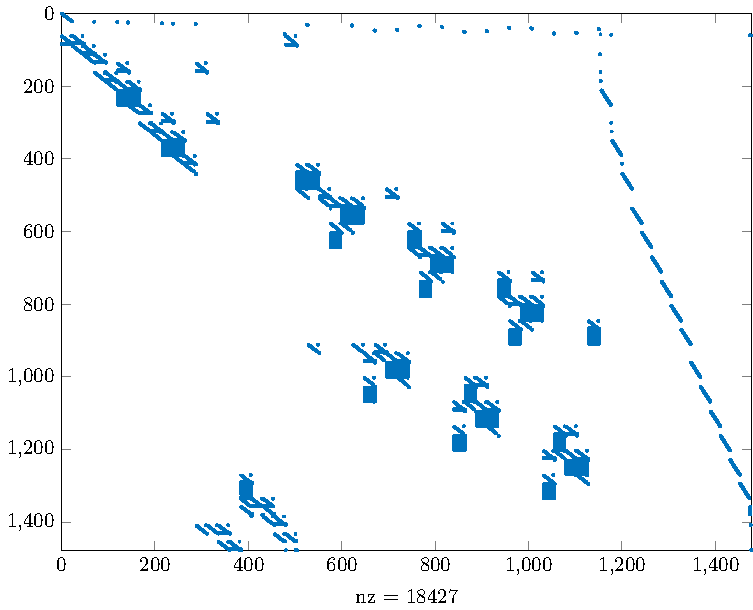
\includegraphics[scale=0.8]{../src/figure/lhr01.pdf}
\caption{Sparsity representation of the \texttt{lhr01} matrix.}
\label{fig:lhr01}
\end{figure}
Figure~\ref{fig:lhr01} shows the sparsity pattern of the \texttt{lhr01} light hydrocarbon recovery matrix. This matrix is real and not symmetric. From a complex point of view it again can be considered non-hermitian. However this matrix is a lot less symmetric then the circuit equations that have been explored earlier. The iterative methods implemented in the provided executable fail. \\ Printing the error message: \\
\texttt{ILU factorization failed on equation 21.} \\
In this case the Gaussian elimination process is unstable. Instabilities could arise if an entry in the L matrix is very large. If the L matrix is then multiplied with the corresponding U, the original A is not obtained \footnote{Numerical Linear Algebra, Trefethen, Bau, page 163}. In our
case an obtained preconditioner would not be usable. The direct solver however is able to solve the problem in $0.009011 s$ using \texttt{7.365 MB}. Interestingly enough the direct solver uses a LU-decomposition as well to solve the problem. The two problems are sightly different the incomplete LU seeks to solve $A \approx LU$. The direct methods attempts to solve $LUx = Pb$. These two problems will be implemented differently. Without looking at the code it is difficult to diagnose the problem.


\subsection{ship003}
\begin{figure}
\centering
% This file was created by matlab2tikz.
% Minimal pgfplots version: 1.3
%
%The latest updates can be retrieved from
%  http://www.mathworks.com/matlabcentral/fileexchange/22022-matlab2tikz
%where you can also make suggestions and rate matlab2tikz.
%
\documentclass[tikz]{standalone}
\usepackage{pgfplots}
\usepackage{grffile}
\pgfplotsset{compat=newest}
\usetikzlibrary{plotmarks}
\usepackage{amsmath}

\begin{document}
\definecolor{mycolor1}{rgb}{0.00000,0.44700,0.74100}%
\definecolor{mycolor2}{rgb}{0.85000,0.32500,0.09800}%
\definecolor{mycolor3}{rgb}{0.92900,0.69400,0.12500}%
\definecolor{mycolor4}{rgb}{0.49400,0.18400,0.55600}%
\definecolor{mycolor5}{rgb}{0.46600,0.67400,0.18800}%
%
\begin{tikzpicture}

\begin{axis}[%
width=4in,
height=3in,
at={(0.947917in,0.629062in)},
scale only axis,
xmode=log,
xmin=1,
xmax=10000,
xminorticks=true,
ymode=log,
ymin=1e-05,
ymax=1e+20,
yminorticks=true,
legend style={legend cell align=left,align=left,draw=white!15!black}
]
\addplot [color=mycolor1,solid]
  table[row sep=crcr]{%
1	80124.1\\
2	26016.3\\
3	20237.5\\
4	20066\\
5	16670.5\\
6	14371.1\\
7	13029.6\\
8	8278.16\\
9	5668.8\\
10	5023.98\\
11	5019.28\\
12	5018.94\\
13	4984.54\\
14	4983.67\\
15	4967.04\\
16	4932.35\\
17	4764.67\\
18	4579.06\\
19	4525.1\\
20	4304.37\\
21	3908.11\\
22	3809.01\\
23	3805.42\\
24	3803.24\\
25	3791.22\\
26	3786.99\\
27	3776.65\\
28	3554.09\\
29	3369.29\\
30	3078.21\\
31	2914.19\\
32	2908.55\\
33	2691.39\\
34	2527.03\\
35	2526.98\\
36	2511.47\\
37	2491.28\\
38	2483.51\\
39	2479.55\\
40	2446.94\\
41	2445\\
42	2444.9\\
43	2440.02\\
44	2439.06\\
45	2433.94\\
46	2415.53\\
47	2392.39\\
48	2364.09\\
49	2359.55\\
50	2342.29\\
51	2237.14\\
52	2155.83\\
53	2149.6\\
54	2130.67\\
55	2106\\
56	2081.28\\
57	2029.64\\
58	1821.16\\
59	1800.02\\
60	1334.82\\
61	1260.3\\
62	1243.16\\
63	1007.37\\
64	977.592\\
65	956.32\\
66	940.22\\
67	869.446\\
68	750.212\\
69	738.274\\
70	722.974\\
71	639.208\\
72	628.897\\
73	625.205\\
74	623.778\\
75	623.237\\
76	621.776\\
77	617.353\\
78	562.33\\
79	439.765\\
80	425.231\\
81	392.7\\
82	366.05\\
83	361.033\\
84	323.718\\
85	307.799\\
86	304.184\\
87	281.243\\
88	263.974\\
89	261.666\\
90	219.682\\
91	210.979\\
92	209.713\\
93	196.812\\
94	196.341\\
95	196.122\\
96	195.585\\
97	194.395\\
98	192.123\\
99	191.575\\
100	191.434\\
101	191.041\\
102	191.014\\
103	190.952\\
104	190.946\\
105	190.931\\
106	190.876\\
107	189.729\\
108	190.816\\
109	189.362\\
110	188.719\\
111	187.299\\
112	187.08\\
113	186.746\\
114	186.565\\
115	186.54\\
116	186.507\\
117	185.19\\
118	184.36\\
119	178.081\\
120	175.545\\
121	175.403\\
122	175.384\\
123	174.598\\
124	174.097\\
125	174.045\\
126	173.857\\
127	172.974\\
128	172.378\\
129	171.384\\
130	168.114\\
131	167.959\\
132	167.922\\
133	165.88\\
134	165.509\\
135	165.503\\
136	165.452\\
137	165.433\\
138	165.422\\
139	165.327\\
140	163.868\\
141	163.832\\
142	163.826\\
143	163.286\\
144	163.202\\
145	163.166\\
146	162.984\\
147	162.908\\
148	162.651\\
149	162.519\\
150	160.795\\
151	160.572\\
152	160.539\\
153	159.431\\
154	159.095\\
155	159.085\\
156	159.066\\
157	159.066\\
158	159.066\\
159	159.005\\
160	158.033\\
161	158.014\\
162	158.011\\
163	157.546\\
164	157.51\\
165	157.386\\
166	157.18\\
167	157.179\\
168	157.054\\
169	156.96\\
170	155.952\\
171	155.73\\
172	155.709\\
173	154.916\\
174	154.845\\
175	154.78\\
176	154.688\\
177	154.688\\
178	154.683\\
179	154.647\\
180	153.976\\
181	153.875\\
182	153.866\\
183	153.562\\
184	153.525\\
185	153.443\\
186	153.281\\
187	153.263\\
188	153.216\\
189	153.159\\
190	152.319\\
191	152.149\\
192	152.132\\
193	151.429\\
194	151.38\\
195	151.322\\
196	151.261\\
197	151.258\\
198	151.248\\
199	151.18\\
200	150.652\\
201	150.592\\
202	150.587\\
203	150.321\\
204	150.315\\
205	150.19\\
206	150.064\\
207	150.061\\
208	150.017\\
209	149.975\\
210	149.306\\
211	149.1\\
212	149.082\\
213	148.452\\
214	148.388\\
215	148.356\\
216	148.309\\
217	148.308\\
218	148.301\\
219	148.247\\
220	147.752\\
221	147.714\\
222	147.711\\
223	147.466\\
224	147.466\\
225	147.331\\
226	147.221\\
227	147.22\\
228	147.187\\
229	147.154\\
230	146.556\\
231	146.351\\
232	146.333\\
233	145.733\\
234	145.675\\
235	145.644\\
236	145.608\\
237	145.607\\
238	145.601\\
239	145.559\\
240	145.086\\
241	145.059\\
242	145.057\\
243	144.835\\
244	144.834\\
245	144.694\\
246	144.594\\
247	144.594\\
248	144.567\\
249	144.538\\
250	143.982\\
251	143.776\\
252	143.758\\
253	143.179\\
254	143.122\\
255	143.088\\
256	143.061\\
257	143.06\\
258	143.054\\
259	143.017\\
260	142.563\\
261	142.544\\
262	142.543\\
263	142.344\\
264	142.339\\
265	142.199\\
266	142.1\\
267	142.1\\
268	142.078\\
269	142.05\\
270	141.527\\
271	141.314\\
272	141.296\\
273	140.738\\
274	140.676\\
275	140.636\\
276	140.618\\
277	140.617\\
278	140.611\\
279	140.567\\
280	140.136\\
281	140.124\\
282	140.123\\
283	139.95\\
284	139.939\\
285	139.8\\
286	139.696\\
287	139.696\\
288	139.678\\
289	139.652\\
290	139.154\\
291	138.934\\
292	138.916\\
293	138.372\\
294	138.316\\
295	138.264\\
296	138.254\\
297	138.253\\
298	138.247\\
299	138.19\\
300	137.784\\
301	137.778\\
302	137.778\\
303	137.632\\
304	137.61\\
305	137.467\\
306	137.364\\
307	137.364\\
308	137.347\\
309	137.325\\
310	136.842\\
311	136.619\\
312	136.6\\
313	136.066\\
314	136.014\\
315	135.953\\
316	135.95\\
317	135.949\\
318	135.943\\
319	135.888\\
320	135.491\\
321	135.489\\
322	135.489\\
323	135.367\\
324	135.338\\
325	135.191\\
326	135.085\\
327	135.085\\
328	135.07\\
329	135.049\\
330	134.573\\
331	134.356\\
332	134.338\\
333	133.806\\
334	133.759\\
335	133.695\\
336	133.695\\
337	133.695\\
338	133.687\\
339	133.637\\
340	133.253\\
341	133.251\\
342	133.251\\
343	133.139\\
344	133.119\\
345	132.973\\
346	132.867\\
347	132.867\\
348	132.854\\
349	132.842\\
350	132.37\\
351	132.143\\
352	132.122\\
353	131.602\\
354	131.503\\
355	131.497\\
356	131.497\\
357	131.497\\
358	131.494\\
359	131.455\\
360	131.095\\
361	131.086\\
362	131.085\\
363	130.913\\
364	130.911\\
365	130.808\\
366	130.726\\
367	130.725\\
368	130.704\\
369	130.688\\
370	130.148\\
371	130.011\\
372	130.001\\
373	129.523\\
374	129.501\\
375	129.359\\
376	129.357\\
377	129.356\\
378	129.354\\
379	129.324\\
380	129.001\\
381	128.984\\
382	128.982\\
383	128.82\\
384	128.813\\
385	128.745\\
386	128.677\\
387	128.676\\
388	128.661\\
389	128.651\\
390	128.096\\
391	127.956\\
392	127.944\\
393	127.451\\
394	127.393\\
395	127.301\\
396	127.298\\
397	127.294\\
398	127.29\\
399	127.257\\
400	126.948\\
401	126.945\\
402	126.945\\
403	126.801\\
404	126.798\\
405	126.695\\
406	126.638\\
407	126.637\\
408	126.622\\
409	126.616\\
410	126.103\\
411	125.935\\
412	125.919\\
413	125.423\\
414	125.364\\
415	125.315\\
416	125.305\\
417	125.304\\
418	125.301\\
419	125.288\\
420	124.949\\
421	124.946\\
422	124.946\\
423	124.795\\
424	124.787\\
425	124.677\\
426	124.63\\
427	124.629\\
428	124.612\\
429	124.602\\
430	124.076\\
431	123.949\\
432	123.936\\
433	123.457\\
434	123.435\\
435	123.341\\
436	123.326\\
437	123.324\\
438	123.319\\
439	123.306\\
440	122.979\\
441	122.975\\
442	122.975\\
443	122.834\\
444	122.819\\
445	122.712\\
446	122.671\\
447	122.671\\
448	122.658\\
449	122.653\\
450	122.121\\
451	121.998\\
452	121.982\\
453	121.516\\
454	121.493\\
455	121.409\\
456	121.389\\
457	121.388\\
458	121.383\\
459	121.371\\
460	121.035\\
461	121.034\\
462	121.034\\
463	120.897\\
464	120.871\\
465	120.757\\
466	120.72\\
467	120.719\\
468	120.708\\
469	120.702\\
470	120.182\\
471	120.064\\
472	120.047\\
473	119.602\\
474	119.586\\
475	119.496\\
476	119.472\\
477	119.471\\
478	119.463\\
479	119.45\\
480	119.103\\
481	119.103\\
482	119.103\\
483	118.971\\
484	118.933\\
485	118.808\\
486	118.773\\
487	118.771\\
488	118.764\\
489	118.76\\
490	118.263\\
491	118.131\\
492	118.112\\
493	117.688\\
494	117.671\\
495	117.591\\
496	117.562\\
497	117.562\\
498	117.551\\
499	117.535\\
500	117.16\\
501	117.158\\
502	117.158\\
503	117.021\\
504	116.964\\
505	116.817\\
506	116.786\\
507	116.781\\
508	116.777\\
509	116.775\\
510	116.309\\
511	116.167\\
512	116.146\\
513	115.759\\
514	115.754\\
515	115.656\\
516	115.625\\
517	115.625\\
518	115.603\\
519	115.582\\
520	115.159\\
521	115.144\\
522	115.142\\
523	115.017\\
524	114.92\\
525	114.734\\
526	114.7\\
527	114.694\\
528	114.693\\
529	114.693\\
530	114.252\\
531	114.078\\
532	114.049\\
533	113.704\\
534	113.69\\
535	113.618\\
536	113.579\\
537	113.574\\
538	113.539\\
539	113.503\\
540	112.998\\
541	112.973\\
542	112.97\\
543	112.644\\
544	112.591\\
545	112.416\\
546	112.381\\
547	112.353\\
548	112.352\\
549	112.351\\
550	111.923\\
551	111.752\\
552	111.727\\
553	111.578\\
554	111.485\\
555	111.339\\
556	111.288\\
557	111.258\\
558	111.206\\
559	111.047\\
560	110.499\\
561	110.395\\
562	110.386\\
563	110.347\\
564	109.95\\
565	109.61\\
566	109.572\\
567	109.543\\
568	109.528\\
569	109.525\\
570	109.307\\
571	109.096\\
572	109.077\\
573	109.07\\
574	108.826\\
575	108.745\\
576	108.729\\
577	108.691\\
578	108.599\\
579	108.14\\
580	107.76\\
581	107.314\\
582	107.255\\
583	107.16\\
584	106.644\\
585	105.895\\
586	105.88\\
587	105.801\\
588	105.698\\
589	105.654\\
590	105.619\\
591	105.112\\
592	105.094\\
593	105.093\\
594	104.887\\
595	104.809\\
596	104.794\\
597	104.78\\
598	104.435\\
599	104.209\\
600	102.849\\
601	102.694\\
602	102.679\\
603	102.556\\
604	102.09\\
605	101.44\\
606	101.336\\
607	101.336\\
608	101.202\\
609	101.194\\
610	101.123\\
611	101.011\\
612	101.009\\
613	100.989\\
614	100.923\\
615	100.875\\
616	100.843\\
617	100.746\\
618	100.729\\
619	100.471\\
620	100.109\\
621	100.027\\
622	100.014\\
623	99.9339\\
624	99.798\\
625	99.3436\\
626	99.3361\\
627	99.3275\\
628	99.2776\\
629	99.266\\
630	99.1908\\
631	98.9766\\
632	98.9716\\
633	98.969\\
634	98.8722\\
635	98.8239\\
636	98.8057\\
637	98.7852\\
638	98.65\\
639	98.5653\\
640	97.9033\\
641	97.6781\\
642	97.6515\\
643	97.557\\
644	97.3509\\
645	96.6555\\
646	96.6328\\
647	96.5196\\
648	96.4722\\
649	96.3733\\
650	96.3023\\
651	96.0122\\
652	95.9935\\
653	95.9925\\
654	95.9267\\
655	95.9088\\
656	95.9062\\
657	95.8352\\
658	95.5808\\
659	95.3291\\
660	94.4194\\
661	93.0871\\
662	92.7702\\
663	92.1027\\
664	92.0757\\
665	91.3137\\
666	91.1564\\
667	91.1394\\
668	90.8209\\
669	90.8156\\
670	90.8154\\
671	90.6783\\
672	90.6782\\
673	90.6085\\
674	90.6029\\
675	90.5996\\
676	90.5996\\
677	90.5807\\
678	90.3664\\
679	90.3529\\
680	89.7171\\
681	89.5988\\
682	89.5912\\
683	88.9872\\
684	88.9861\\
685	88.9243\\
686	88.901\\
687	88.8477\\
688	88.8472\\
689	88.8415\\
690	88.6325\\
691	88.5746\\
692	88.5641\\
693	88.4621\\
694	88.4618\\
695	88.4226\\
696	88.4026\\
697	88.402\\
698	88.3393\\
699	88.325\\
700	87.9012\\
701	87.8023\\
702	87.7968\\
703	87.396\\
704	87.3747\\
705	87.3463\\
706	87.3443\\
707	87.3382\\
708	87.3381\\
709	87.3379\\
710	87.1693\\
711	87.1653\\
712	87.1649\\
713	87.094\\
714	87.094\\
715	87.0676\\
716	87.0512\\
717	87.0508\\
718	86.9929\\
719	86.9846\\
720	86.4891\\
721	86.4885\\
722	86.4885\\
723	86.1253\\
724	86.0319\\
725	86.0195\\
726	86.0194\\
727	86.0099\\
728	86.0092\\
729	86.0092\\
730	85.9083\\
731	85.8536\\
732	85.8506\\
733	85.8134\\
734	85.8126\\
735	85.7935\\
736	85.7809\\
737	85.7713\\
738	85.7178\\
739	85.7076\\
740	85.1958\\
741	85.1931\\
742	85.1928\\
743	84.8174\\
744	84.7512\\
745	84.6697\\
746	84.663\\
747	84.6562\\
748	84.6546\\
749	84.6546\\
750	84.5729\\
751	84.5257\\
752	84.5244\\
753	84.4999\\
754	84.4869\\
755	84.4634\\
756	84.4553\\
757	84.4531\\
758	84.3877\\
759	84.3788\\
760	83.9389\\
761	83.8979\\
762	83.8942\\
763	83.5169\\
764	83.4981\\
765	83.4543\\
766	83.4537\\
767	83.4516\\
768	83.4512\\
769	83.4379\\
770	83.3023\\
771	83.3023\\
772	83.3023\\
773	83.2617\\
774	83.2478\\
775	83.2055\\
776	83.1788\\
777	83.1784\\
778	83.1512\\
779	83.1403\\
780	82.8321\\
781	82.7435\\
782	82.7347\\
783	82.4339\\
784	82.4187\\
785	82.372\\
786	82.372\\
787	82.3715\\
788	82.3708\\
789	82.3632\\
790	82.2156\\
791	82.2067\\
792	82.2059\\
793	82.1713\\
794	82.156\\
795	82.1148\\
796	82.094\\
797	82.0933\\
798	82.0656\\
799	82.0482\\
800	81.6822\\
801	81.6574\\
802	81.6544\\
803	81.3401\\
804	81.3401\\
805	81.2634\\
806	81.2633\\
807	81.2603\\
808	81.2603\\
809	81.257\\
810	81.1337\\
811	81.1139\\
812	81.1123\\
813	81.0846\\
814	81.0698\\
815	81.0379\\
816	81.0247\\
817	81.0217\\
818	80.9869\\
819	80.9748\\
820	80.5433\\
821	80.5383\\
822	80.5376\\
823	80.1792\\
824	80.1642\\
825	80.0909\\
826	80.0906\\
827	80.0781\\
828	80.0769\\
829	80.0769\\
830	79.986\\
831	79.9271\\
832	79.9213\\
833	79.9061\\
834	79.8963\\
835	79.8805\\
836	79.8753\\
837	79.8612\\
838	79.8013\\
839	79.7757\\
840	79.2637\\
841	79.2631\\
842	79.263\\
843	78.9333\\
844	78.8806\\
845	78.7658\\
846	78.7632\\
847	78.7513\\
848	78.746\\
849	78.7314\\
850	78.6415\\
851	78.6388\\
852	78.6385\\
853	78.5981\\
854	78.5924\\
855	78.5581\\
856	78.5437\\
857	78.5382\\
858	78.5099\\
859	78.4606\\
860	78.1443\\
861	78.1052\\
862	78.0999\\
863	77.8382\\
864	77.8182\\
865	77.7306\\
866	77.7261\\
867	77.7167\\
868	77.7167\\
869	77.7166\\
870	77.6443\\
871	77.5519\\
872	77.5436\\
873	77.5266\\
874	77.5213\\
875	77.5022\\
876	77.4966\\
877	77.47\\
878	77.4414\\
879	77.3972\\
880	77.1667\\
881	77.1027\\
882	77.099\\
883	76.9325\\
884	76.9094\\
885	76.8558\\
886	76.8453\\
887	76.842\\
888	76.8414\\
889	76.768\\
890	76.5992\\
891	76.4846\\
892	76.4643\\
893	76.3431\\
894	76.2852\\
895	76.2616\\
896	76.1465\\
897	76.1314\\
898	76.1279\\
899	76.1221\\
900	76.0601\\
901	75.886\\
902	75.8718\\
903	75.7675\\
904	75.7407\\
905	75.7359\\
906	75.7329\\
907	75.7236\\
908	75.6742\\
909	75.6288\\
910	75.4963\\
911	75.4598\\
912	75.4592\\
913	75.3928\\
914	75.3886\\
915	75.369\\
916	75.3547\\
917	75.3418\\
918	75.3386\\
919	75.2408\\
920	74.8562\\
921	74.8538\\
922	74.8534\\
923	74.6168\\
924	74.528\\
925	74.52\\
926	74.5119\\
927	74.5116\\
928	74.5043\\
929	74.4696\\
930	74.3169\\
931	74.3056\\
932	74.3051\\
933	74.2161\\
934	74.2116\\
935	74.1833\\
936	74.1669\\
937	74.1669\\
938	74.1606\\
939	74.1581\\
940	73.8653\\
941	73.8412\\
942	73.8374\\
943	73.6364\\
944	73.5971\\
945	73.5835\\
946	73.5755\\
947	73.5755\\
948	73.5643\\
949	73.5512\\
950	73.3819\\
951	73.3795\\
952	73.3791\\
953	73.2727\\
954	73.2621\\
955	73.2382\\
956	73.2127\\
957	73.2127\\
958	73.2111\\
959	73.1943\\
960	72.8981\\
961	72.8896\\
962	72.8881\\
963	72.646\\
964	72.5907\\
965	72.5834\\
966	72.5736\\
967	72.5729\\
968	72.5725\\
969	72.5717\\
970	72.4757\\
971	72.4249\\
972	72.42\\
973	72.3739\\
974	72.368\\
975	72.3598\\
976	72.3461\\
977	72.345\\
978	72.3283\\
979	72.3269\\
980	72.0743\\
981	72.0053\\
982	72.0007\\
983	71.7812\\
984	71.7539\\
985	71.7441\\
986	71.7325\\
987	71.7325\\
988	71.7302\\
989	71.7135\\
990	71.5744\\
991	71.5659\\
992	71.5645\\
993	71.4917\\
994	71.4674\\
995	71.4581\\
996	71.4074\\
997	71.4072\\
998	71.4056\\
999	71.4026\\
1000	71.1731\\
1001	71.1267\\
1002	71.121\\
1003	70.9104\\
1004	70.8795\\
1005	70.8763\\
1006	70.8677\\
1007	70.8677\\
1008	70.863\\
1009	70.8394\\
1010	70.7142\\
1011	70.714\\
};
\addlegendentry{gmres(0,10)};

\addplot [color=mycolor2,solid]
  table[row sep=crcr]{%
1	80124.1\\
2	26016.3\\
3	20237.5\\
4	20066\\
5	16670.5\\
6	14371.1\\
7	13029.6\\
8	8278.16\\
9	5668.8\\
10	5023.98\\
11	5019.28\\
12	4782.67\\
13	4298.53\\
14	3922.89\\
15	3720.88\\
16	3702.59\\
17	3349.54\\
18	2687.67\\
19	1701.82\\
20	1552.88\\
21	1460.08\\
22	958.291\\
23	683.209\\
24	617.872\\
25	598.742\\
26	381.897\\
27	267.32\\
28	218.621\\
29	188.899\\
30	139.883\\
31	111.946\\
32	95.9056\\
33	92.8032\\
34	87.2332\\
35	81.1724\\
36	78.4796\\
37	76.1831\\
38	73.9077\\
39	70.6936\\
40	68.7545\\
41	63.0108\\
42	54.1183\\
43	49.5625\\
44	45.873\\
45	41.8852\\
46	38.7496\\
47	34.805\\
48	30.7031\\
49	25.5082\\
50	22.3299\\
51	20.709\\
52	19.2167\\
53	18.2916\\
54	17.6902\\
55	17.1439\\
56	15.8218\\
57	14.4612\\
58	13.5534\\
59	12.7434\\
60	11.6816\\
61	11.0311\\
62	10.3777\\
63	9.98344\\
64	9.75775\\
65	9.42888\\
66	8.95829\\
67	8.46746\\
68	7.90574\\
69	7.54639\\
70	7.21813\\
71	6.89903\\
72	6.59136\\
73	6.34847\\
74	5.9897\\
75	5.60317\\
76	5.12845\\
77	4.80033\\
78	4.52733\\
79	4.30437\\
80	4.1068\\
81	3.93526\\
82	3.72056\\
83	3.50275\\
84	3.34289\\
85	3.22604\\
86	3.07965\\
87	2.968\\
88	2.88472\\
89	2.76239\\
90	2.6468\\
91	2.54954\\
92	2.41235\\
93	2.33261\\
94	2.28053\\
95	2.22262\\
96	2.1143\\
97	2.02295\\
98	1.93788\\
99	1.85467\\
100	1.77364\\
101	1.68043\\
102	1.68043\\
103	1.68042\\
104	1.68042\\
105	1.68042\\
106	1.68042\\
107	1.68042\\
108	1.68041\\
109	1.6804\\
110	1.68039\\
111	1.68038\\
112	1.68038\\
113	1.68037\\
114	1.68037\\
115	1.68036\\
116	1.68036\\
117	1.68036\\
118	1.68036\\
119	1.68035\\
120	1.68034\\
121	1.68034\\
122	1.68032\\
123	1.68024\\
124	1.68004\\
125	1.67983\\
126	1.67983\\
127	1.67935\\
128	1.67855\\
129	1.67785\\
130	1.67741\\
131	1.67648\\
132	1.67597\\
133	1.67563\\
134	1.67416\\
135	1.66997\\
136	1.66721\\
137	1.66679\\
138	1.6667\\
139	1.66667\\
140	1.66665\\
141	1.66665\\
142	1.66639\\
143	1.66569\\
144	1.66558\\
145	1.66557\\
146	1.66524\\
147	1.66509\\
148	1.66495\\
149	1.66426\\
150	1.66223\\
151	1.66052\\
152	1.65938\\
153	1.65719\\
154	1.65542\\
155	1.65365\\
156	1.64972\\
157	1.6378\\
158	1.62069\\
159	1.60743\\
160	1.59439\\
161	1.57703\\
162	1.56294\\
163	1.54927\\
164	1.53959\\
165	1.53567\\
166	1.52907\\
167	1.52151\\
168	1.51137\\
169	1.50017\\
170	1.49307\\
171	1.48679\\
172	1.47752\\
173	1.46831\\
174	1.4591\\
175	1.43897\\
176	1.41567\\
177	1.37648\\
178	1.34394\\
179	1.31033\\
180	1.28971\\
181	1.2616\\
182	1.24114\\
183	1.20856\\
184	1.16399\\
185	1.11899\\
186	1.08532\\
187	1.04122\\
188	0.999281\\
189	0.977005\\
190	0.9393\\
191	0.907699\\
192	0.88103\\
193	0.847901\\
194	0.808002\\
195	0.792031\\
196	0.768599\\
197	0.725579\\
198	0.680918\\
199	0.645037\\
200	0.587153\\
201	0.531211\\
202	0.531205\\
203	0.531205\\
204	0.531204\\
205	0.531204\\
206	0.531204\\
207	0.531203\\
208	0.5312\\
209	0.5312\\
210	0.531198\\
211	0.531195\\
212	0.531195\\
213	0.531189\\
214	0.531184\\
215	0.531182\\
216	0.531182\\
217	0.531181\\
218	0.531179\\
219	0.531174\\
220	0.53117\\
221	0.531165\\
222	0.531165\\
223	0.531148\\
224	0.531101\\
225	0.531025\\
226	0.530996\\
227	0.53092\\
228	0.530739\\
229	0.530619\\
230	0.530517\\
231	0.530108\\
232	0.529648\\
233	0.529097\\
234	0.528772\\
235	0.528772\\
236	0.528646\\
237	0.528608\\
238	0.528602\\
239	0.528601\\
240	0.528601\\
241	0.528601\\
242	0.52856\\
243	0.528481\\
244	0.528477\\
245	0.528475\\
246	0.52846\\
247	0.528422\\
248	0.52842\\
249	0.528351\\
250	0.528112\\
251	0.52798\\
252	0.527907\\
253	0.527717\\
254	0.52759\\
255	0.527471\\
256	0.527133\\
257	0.526029\\
258	0.524537\\
259	0.523466\\
260	0.522451\\
261	0.521216\\
262	0.520049\\
263	0.518786\\
264	0.517789\\
265	0.517165\\
266	0.516286\\
267	0.515276\\
268	0.514235\\
269	0.513216\\
270	0.51274\\
271	0.512423\\
272	0.511982\\
273	0.5117\\
274	0.511344\\
275	0.510318\\
276	0.509145\\
277	0.506795\\
278	0.504413\\
279	0.502752\\
280	0.500908\\
281	0.499497\\
282	0.497516\\
283	0.495826\\
284	0.492421\\
285	0.489662\\
286	0.487843\\
287	0.484935\\
288	0.482301\\
289	0.480488\\
290	0.477127\\
291	0.472301\\
292	0.469769\\
293	0.464373\\
294	0.460473\\
295	0.457996\\
296	0.455046\\
297	0.446778\\
298	0.43935\\
299	0.433127\\
300	0.423857\\
301	0.415383\\
302	0.415381\\
303	0.41538\\
304	0.415379\\
305	0.415379\\
306	0.415378\\
307	0.415378\\
308	0.415375\\
309	0.415374\\
310	0.415373\\
311	0.415372\\
312	0.41537\\
313	0.415365\\
314	0.41536\\
315	0.415359\\
316	0.415359\\
317	0.415358\\
318	0.415355\\
319	0.415351\\
320	0.415349\\
321	0.415349\\
322	0.415342\\
323	0.415312\\
324	0.415278\\
325	0.415277\\
326	0.415242\\
327	0.41502\\
328	0.414736\\
329	0.414584\\
330	0.414508\\
331	0.414441\\
332	0.414435\\
333	0.414147\\
334	0.413513\\
335	0.412528\\
336	0.411939\\
337	0.411859\\
338	0.411858\\
339	0.411846\\
340	0.411838\\
341	0.411838\\
342	0.411817\\
343	0.411715\\
344	0.411715\\
345	0.411714\\
346	0.411713\\
347	0.411649\\
348	0.411638\\
349	0.41153\\
350	0.411186\\
351	0.410941\\
352	0.410799\\
353	0.410444\\
354	0.410226\\
355	0.410013\\
356	0.409545\\
357	0.408067\\
358	0.406163\\
359	0.404859\\
360	0.403594\\
361	0.401976\\
362	0.40031\\
363	0.398515\\
364	0.396728\\
365	0.395607\\
366	0.393744\\
367	0.39179\\
368	0.389904\\
369	0.388289\\
370	0.387512\\
371	0.387229\\
372	0.386846\\
373	0.386637\\
374	0.386249\\
375	0.385301\\
376	0.383807\\
377	0.381245\\
378	0.377943\\
379	0.375241\\
380	0.372047\\
381	0.368388\\
382	0.365373\\
383	0.360713\\
384	0.355526\\
385	0.350667\\
386	0.348115\\
387	0.343741\\
388	0.33964\\
389	0.336558\\
390	0.330183\\
391	0.322488\\
392	0.316606\\
393	0.308383\\
394	0.301496\\
395	0.29812\\
396	0.293957\\
397	0.282352\\
398	0.26922\\
399	0.25721\\
400	0.241715\\
401	0.228289\\
402	0.228286\\
403	0.228283\\
404	0.228281\\
405	0.22828\\
406	0.228278\\
407	0.228276\\
408	0.22827\\
409	0.228266\\
410	0.228254\\
411	0.228218\\
412	0.228209\\
413	0.228209\\
414	0.228207\\
415	0.228201\\
416	0.228188\\
417	0.228171\\
418	0.228171\\
419	0.228159\\
420	0.228133\\
421	0.228124\\
422	0.228079\\
423	0.227981\\
424	0.227959\\
425	0.227936\\
426	0.227749\\
427	0.227029\\
428	0.225997\\
429	0.225085\\
430	0.224747\\
431	0.224714\\
432	0.224624\\
433	0.223097\\
434	0.22083\\
435	0.216932\\
436	0.214987\\
437	0.214749\\
438	0.214716\\
439	0.214677\\
440	0.214643\\
441	0.214628\\
442	0.214156\\
443	0.21305\\
444	0.212655\\
445	0.21244\\
446	0.211805\\
447	0.211194\\
448	0.210508\\
449	0.208471\\
450	0.204861\\
451	0.202297\\
452	0.200884\\
453	0.198726\\
454	0.19701\\
455	0.195496\\
456	0.192125\\
457	0.18482\\
458	0.177793\\
459	0.173411\\
460	0.169094\\
461	0.162446\\
462	0.157173\\
463	0.151148\\
464	0.147461\\
465	0.145341\\
466	0.142255\\
467	0.138462\\
468	0.133796\\
469	0.128483\\
470	0.125554\\
471	0.123508\\
472	0.121206\\
473	0.119884\\
474	0.118686\\
475	0.115309\\
476	0.111922\\
477	0.107267\\
478	0.104205\\
479	0.101507\\
480	0.100641\\
481	0.0992741\\
482	0.0971261\\
483	0.0941994\\
484	0.0896043\\
485	0.0849542\\
486	0.0825328\\
487	0.080125\\
488	0.0779618\\
489	0.0771032\\
490	0.0752073\\
491	0.0733852\\
492	0.0725216\\
493	0.0710267\\
494	0.069291\\
495	0.0680036\\
496	0.0664778\\
497	0.0636574\\
498	0.0622239\\
499	0.0613678\\
500	0.0603686\\
501	0.059357\\
502	0.0593558\\
503	0.0593546\\
504	0.0593535\\
505	0.0593534\\
506	0.0593533\\
507	0.059353\\
508	0.059352\\
509	0.059351\\
510	0.0593475\\
511	0.0593372\\
512	0.0593327\\
513	0.0593322\\
514	0.0593317\\
515	0.0593297\\
516	0.059325\\
517	0.0593203\\
518	0.0593186\\
519	0.0593052\\
520	0.0592804\\
521	0.0592451\\
522	0.0592443\\
523	0.0592096\\
524	0.0591826\\
525	0.0591825\\
526	0.0591634\\
527	0.0590203\\
528	0.0588523\\
529	0.0588381\\
530	0.0587645\\
531	0.0585298\\
532	0.0582914\\
533	0.0577271\\
534	0.0571086\\
535	0.05646\\
536	0.0559487\\
537	0.0558434\\
538	0.055831\\
539	0.0558115\\
540	0.0558026\\
541	0.0558018\\
542	0.0557062\\
543	0.055488\\
544	0.0554155\\
545	0.0553583\\
546	0.0552738\\
547	0.0552079\\
548	0.0551605\\
549	0.0549001\\
550	0.0545213\\
551	0.0543223\\
552	0.054137\\
553	0.0538252\\
554	0.0536291\\
555	0.0532905\\
556	0.0526086\\
557	0.0515579\\
558	0.0506982\\
559	0.0502083\\
560	0.0498839\\
561	0.0494409\\
562	0.0489726\\
563	0.0485714\\
564	0.0483077\\
565	0.0481187\\
566	0.0478907\\
567	0.0475753\\
568	0.0473029\\
569	0.0470223\\
570	0.0468304\\
571	0.0466654\\
572	0.04651\\
573	0.0463523\\
574	0.0462129\\
575	0.0458946\\
576	0.0455844\\
577	0.0450813\\
578	0.0448149\\
579	0.0443941\\
580	0.0440767\\
581	0.043627\\
582	0.0433682\\
583	0.0429509\\
584	0.0426224\\
585	0.0423492\\
586	0.0421236\\
587	0.0418138\\
588	0.0415774\\
589	0.0413242\\
590	0.0410529\\
591	0.0408304\\
592	0.0406389\\
593	0.0404142\\
594	0.0403073\\
595	0.0402269\\
596	0.0401411\\
597	0.0399818\\
598	0.0397168\\
599	0.0393429\\
600	0.0389747\\
601	0.0385579\\
602	0.0385556\\
603	0.0385554\\
604	0.0385549\\
605	0.0385545\\
606	0.0385541\\
607	0.0385534\\
608	0.0385506\\
609	0.0385493\\
610	0.0385491\\
611	0.0385488\\
612	0.0385479\\
613	0.0385449\\
614	0.0385445\\
615	0.0385436\\
616	0.0385409\\
617	0.0385397\\
618	0.0385392\\
619	0.038538\\
620	0.0385349\\
621	0.0385329\\
622	0.0385327\\
623	0.038531\\
624	0.0385174\\
625	0.038488\\
626	0.0384394\\
627	0.0384179\\
628	0.0384131\\
629	0.0383361\\
630	0.0382452\\
631	0.0381966\\
632	0.0381467\\
633	0.038062\\
634	0.0379645\\
635	0.0378761\\
636	0.0378096\\
637	0.0377539\\
638	0.0376956\\
639	0.037619\\
640	0.0375559\\
641	0.0375116\\
642	0.0374566\\
643	0.0373693\\
644	0.0373159\\
645	0.0372755\\
646	0.0372348\\
647	0.0371813\\
648	0.0371598\\
649	0.0371131\\
650	0.0370775\\
651	0.0370512\\
652	0.0369994\\
653	0.0369126\\
654	0.0368614\\
655	0.0367818\\
656	0.0366616\\
657	0.0365235\\
658	0.0363866\\
659	0.0363075\\
660	0.0362509\\
661	0.0361649\\
662	0.0360546\\
663	0.0359736\\
664	0.035912\\
665	0.0358363\\
666	0.0357541\\
667	0.0356746\\
668	0.0356302\\
669	0.0355508\\
670	0.0354721\\
671	0.0354215\\
672	0.035383\\
673	0.0353158\\
674	0.0352042\\
675	0.0350586\\
676	0.034865\\
677	0.0347682\\
678	0.0346904\\
679	0.0346314\\
680	0.0345357\\
681	0.0343839\\
682	0.0342055\\
683	0.0339622\\
684	0.0337993\\
685	0.0336898\\
686	0.0335736\\
687	0.0333941\\
688	0.0331884\\
689	0.0329998\\
690	0.0327611\\
691	0.0326138\\
692	0.0325101\\
693	0.032429\\
694	0.0322662\\
695	0.0321315\\
696	0.0319922\\
697	0.0318351\\
698	0.0317155\\
699	0.0316491\\
700	0.0315739\\
701	0.0314922\\
702	0.0314881\\
703	0.0314876\\
704	0.0314873\\
705	0.0314858\\
706	0.0314855\\
707	0.0314852\\
708	0.0314852\\
709	0.0314835\\
710	0.0314806\\
711	0.0314806\\
712	0.0314765\\
713	0.0314703\\
714	0.0314695\\
715	0.0314673\\
716	0.0314565\\
717	0.0314549\\
718	0.0314535\\
719	0.0314487\\
720	0.0314438\\
721	0.0314391\\
722	0.0314382\\
723	0.0314287\\
724	0.0314131\\
725	0.0313751\\
726	0.0313353\\
727	0.0313338\\
728	0.0313285\\
729	0.0313069\\
730	0.0312679\\
731	0.0312272\\
732	0.0311866\\
733	0.0311228\\
734	0.0310855\\
735	0.0310505\\
736	0.0310062\\
737	0.0309491\\
738	0.0309013\\
739	0.0308842\\
740	0.0308618\\
741	0.0308418\\
742	0.0308092\\
743	0.030758\\
744	0.0307227\\
745	0.0306921\\
746	0.0306604\\
747	0.0306318\\
748	0.0306163\\
749	0.0306023\\
750	0.0305558\\
751	0.0304988\\
752	0.0304651\\
753	0.0304312\\
754	0.0304192\\
755	0.0303974\\
756	0.0303625\\
757	0.0303287\\
758	0.0302847\\
759	0.0302296\\
760	0.0301921\\
761	0.0301228\\
762	0.0300588\\
763	0.0300143\\
764	0.029937\\
765	0.029852\\
766	0.0298029\\
767	0.0297545\\
768	0.0297133\\
769	0.0296785\\
770	0.0296212\\
771	0.0295905\\
772	0.0295564\\
773	0.0294353\\
774	0.0293504\\
775	0.0293118\\
776	0.0292495\\
777	0.029143\\
778	0.0291131\\
779	0.0290183\\
780	0.0289505\\
781	0.0288124\\
782	0.0286515\\
783	0.0283572\\
784	0.0281393\\
785	0.0280217\\
786	0.0278949\\
787	0.0277885\\
788	0.0276851\\
789	0.0275756\\
790	0.0274619\\
791	0.0273134\\
792	0.0271913\\
793	0.0271031\\
794	0.027015\\
795	0.0269347\\
796	0.0268846\\
797	0.0267906\\
798	0.0267029\\
799	0.0266127\\
800	0.0265454\\
801	0.0264817\\
802	0.0264807\\
803	0.0264807\\
804	0.0264805\\
805	0.0264804\\
806	0.0264804\\
807	0.0264804\\
808	0.0264803\\
809	0.02648\\
810	0.0264799\\
811	0.0264795\\
812	0.0264782\\
813	0.0264772\\
814	0.0264771\\
815	0.0264751\\
816	0.026464\\
817	0.0264633\\
818	0.0264565\\
819	0.0264458\\
820	0.0264426\\
821	0.0264392\\
822	0.0264156\\
823	0.0264006\\
824	0.0263878\\
825	0.0263613\\
826	0.0263589\\
827	0.0263439\\
828	0.0263148\\
829	0.0262788\\
830	0.0262512\\
831	0.0262157\\
832	0.0261887\\
833	0.0261544\\
834	0.0261147\\
835	0.0260806\\
836	0.0260465\\
837	0.0260165\\
838	0.0259641\\
839	0.0259194\\
840	0.0258691\\
841	0.0258142\\
842	0.0257681\\
843	0.0257236\\
844	0.0256936\\
845	0.0256495\\
846	0.0256223\\
847	0.0255721\\
848	0.0255302\\
849	0.0254982\\
850	0.0254667\\
851	0.0254271\\
852	0.0253595\\
853	0.0252579\\
854	0.0252122\\
855	0.0251605\\
856	0.0250295\\
857	0.0249344\\
858	0.0248425\\
859	0.0247614\\
860	0.0246871\\
861	0.0246416\\
862	0.0245885\\
863	0.0245574\\
864	0.0245196\\
865	0.0244433\\
866	0.0243766\\
867	0.0243279\\
868	0.0242871\\
869	0.0242429\\
870	0.0241916\\
871	0.0241542\\
872	0.0241297\\
873	0.0240871\\
874	0.0240148\\
875	0.0239163\\
876	0.023838\\
877	0.023796\\
878	0.0237577\\
879	0.0237383\\
880	0.023709\\
881	0.0236886\\
882	0.0236413\\
883	0.0235758\\
884	0.0235222\\
885	0.0234569\\
886	0.0233956\\
887	0.0233379\\
888	0.0232819\\
889	0.02323\\
890	0.0231999\\
891	0.0231722\\
892	0.023159\\
893	0.023143\\
894	0.0231266\\
895	0.0230875\\
896	0.0230511\\
897	0.0230055\\
898	0.0229735\\
899	0.0229298\\
900	0.0228917\\
901	0.0228289\\
902	0.0228246\\
903	0.0228223\\
904	0.0228221\\
905	0.0228201\\
906	0.0228196\\
907	0.0228196\\
908	0.0228194\\
909	0.022818\\
910	0.022817\\
911	0.0228166\\
912	0.0228136\\
913	0.0228099\\
914	0.0228098\\
915	0.0228008\\
916	0.0227903\\
917	0.0227859\\
918	0.0227856\\
919	0.0227833\\
920	0.0227775\\
921	0.0227751\\
922	0.0227742\\
923	0.0227728\\
924	0.0227707\\
925	0.0227644\\
926	0.0227575\\
927	0.0227574\\
928	0.0227511\\
929	0.0227351\\
930	0.0227232\\
931	0.0227171\\
932	0.0227105\\
933	0.0227022\\
934	0.0226967\\
935	0.0226899\\
936	0.0226821\\
937	0.0226758\\
938	0.0226653\\
939	0.0226541\\
940	0.022637\\
941	0.0226131\\
942	0.0225928\\
943	0.0225746\\
944	0.0225611\\
945	0.022541\\
946	0.0225108\\
947	0.0224629\\
948	0.0224278\\
949	0.0224\\
950	0.0223592\\
951	0.0223116\\
952	0.0222952\\
953	0.0222527\\
954	0.0222033\\
955	0.0221792\\
956	0.0221568\\
957	0.0221199\\
958	0.0220737\\
959	0.0220263\\
960	0.0219993\\
961	0.0219746\\
962	0.0219501\\
963	0.0219129\\
964	0.0218728\\
965	0.021806\\
966	0.0217376\\
967	0.0216675\\
968	0.0216211\\
969	0.0215671\\
970	0.0215245\\
971	0.0214602\\
972	0.0214185\\
973	0.0213713\\
974	0.0213208\\
975	0.0212815\\
976	0.0212546\\
977	0.0212207\\
978	0.0211792\\
979	0.0211323\\
980	0.0210819\\
981	0.0210289\\
982	0.0209897\\
983	0.0209583\\
984	0.0209266\\
985	0.0208887\\
986	0.0208711\\
987	0.0208556\\
988	0.0208236\\
989	0.0207674\\
990	0.0207097\\
991	0.020663\\
992	0.0206211\\
993	0.0205841\\
994	0.0205552\\
995	0.020537\\
996	0.0205164\\
997	0.0204965\\
998	0.0204783\\
999	0.0204427\\
1000	0.020414\\
1001	0.0203905\\
1002	0.0203893\\
1003	0.0203893\\
1004	0.0203882\\
1005	0.0203868\\
1006	0.0203867\\
1007	0.0203867\\
1008	0.0203865\\
1009	0.0203854\\
1010	0.0203847\\
1011	0.0203843\\
1012	0.0203823\\
1013	0.0203796\\
1014	0.0203796\\
1015	0.0203736\\
1016	0.0203688\\
1017	0.0203687\\
1018	0.0203656\\
1019	0.0203562\\
1020	0.0203538\\
1021	0.0203528\\
1022	0.0203469\\
1023	0.0203338\\
1024	0.0203188\\
1025	0.0202987\\
1026	0.02029\\
1027	0.0202868\\
1028	0.0202646\\
1029	0.02024\\
1030	0.0202285\\
1031	0.0202192\\
1032	0.0202048\\
1033	0.0201858\\
1034	0.0201549\\
1035	0.020133\\
1036	0.0201129\\
1037	0.0200827\\
1038	0.0200528\\
1039	0.0200266\\
1040	0.0199928\\
1041	0.0199678\\
1042	0.0199534\\
1043	0.0199314\\
1044	0.0199001\\
1045	0.0198643\\
1046	0.0198269\\
1047	0.0197764\\
1048	0.0197315\\
1049	0.0196968\\
1050	0.0196521\\
1051	0.0196108\\
1052	0.0195892\\
1053	0.019556\\
1054	0.0195305\\
1055	0.0194969\\
1056	0.0194448\\
1057	0.0194046\\
1058	0.0193589\\
1059	0.0193079\\
1060	0.0192719\\
1061	0.0192214\\
1062	0.0191665\\
1063	0.0190972\\
1064	0.0190511\\
1065	0.0190209\\
1066	0.0190019\\
1067	0.0189539\\
1068	0.0189282\\
1069	0.0189121\\
1070	0.0188975\\
1071	0.0188647\\
1072	0.0188535\\
1073	0.0188362\\
1074	0.0188092\\
1075	0.018772\\
1076	0.018726\\
1077	0.0186564\\
1078	0.0186013\\
1079	0.0185474\\
1080	0.0184858\\
1081	0.0184401\\
1082	0.0183996\\
1083	0.0183578\\
1084	0.0183066\\
1085	0.0182611\\
1086	0.0182285\\
1087	0.0182074\\
1088	0.0181827\\
1089	0.0181543\\
1090	0.0181413\\
1091	0.0181236\\
1092	0.0181076\\
1093	0.0180938\\
1094	0.0180805\\
1095	0.0180646\\
1096	0.0180511\\
1097	0.0180371\\
1098	0.0180092\\
1099	0.0179795\\
1100	0.0179603\\
1101	0.0179344\\
};
\addlegendentry{gmres(0,100)};

\addplot [color=mycolor3,solid]
  table[row sep=crcr]{%
1	63094.8\\
2	16987.3\\
3	10681.3\\
4	10631\\
5	7956.6\\
6	4434.76\\
7	2132.26\\
8	1097.98\\
9	634.582\\
10	424.146\\
11	360.389\\
12	360.157\\
13	359.636\\
14	358.682\\
15	358.649\\
16	357.61\\
17	355.689\\
18	343.886\\
19	316.41\\
20	259.042\\
21	200.846\\
22	200.145\\
23	199.884\\
24	197.523\\
25	197.374\\
26	196.997\\
27	196.571\\
28	192.407\\
29	182.165\\
30	154.824\\
31	115.836\\
32	108.439\\
33	106.185\\
34	95.6623\\
35	87.4324\\
36	81.2892\\
37	78.8596\\
38	77.2597\\
39	73.8021\\
40	67.1143\\
41	64.6234\\
42	64.6033\\
43	64.5844\\
44	64.402\\
45	64.3563\\
46	63.9785\\
47	63.9706\\
48	63.8391\\
49	63.4729\\
50	63.0577\\
51	61.5035\\
52	61.4839\\
53	61.4636\\
54	61.2527\\
55	61.2326\\
56	60.6984\\
57	60.4481\\
58	60.3825\\
59	60.3627\\
60	60.3449\\
61	60.3151\\
62	60.3149\\
63	60.3144\\
64	60.312\\
65	60.2991\\
66	60.2844\\
67	60.2762\\
68	60.2396\\
69	60.1735\\
70	60.1476\\
71	59.1667\\
72	59.1087\\
73	58.9409\\
74	58.5702\\
75	58.542\\
76	58.2501\\
77	58.0315\\
78	57.8026\\
79	57.7795\\
80	57.7695\\
81	57.4291\\
82	57.4258\\
83	57.4151\\
84	57.3322\\
85	57.3198\\
86	57.2972\\
87	57.2971\\
88	57.1536\\
89	56.7744\\
90	56.5955\\
91	56.3632\\
92	56.3605\\
93	56.3546\\
94	56.1712\\
95	56.1666\\
96	56.0227\\
97	55.8626\\
98	55.6928\\
99	55.6901\\
100	55.6247\\
101	55.4049\\
102	55.4019\\
103	55.393\\
104	55.2821\\
105	55.282\\
106	55.2548\\
107	55.2542\\
108	55.2058\\
109	55.1135\\
110	54.862\\
111	54.6381\\
112	54.6357\\
113	54.6295\\
114	54.4857\\
115	54.4846\\
116	54.3776\\
117	54.2648\\
118	54.2134\\
119	54.2113\\
120	54.121\\
121	53.7102\\
122	53.7037\\
123	53.6841\\
124	53.5654\\
125	53.5636\\
126	53.5185\\
127	53.5184\\
128	53.5184\\
129	53.4356\\
130	53.2218\\
131	52.9849\\
132	52.9833\\
133	52.9786\\
134	52.9158\\
135	52.9144\\
136	52.793\\
137	52.6848\\
138	52.6581\\
139	52.6543\\
140	52.6131\\
141	52.3968\\
142	52.3953\\
143	52.392\\
144	52.3405\\
145	52.32\\
146	52.2865\\
147	52.2823\\
148	52.2749\\
149	52.1974\\
150	52.0308\\
151	51.8658\\
152	51.865\\
153	51.8629\\
154	51.824\\
155	51.8128\\
156	51.728\\
157	51.6516\\
158	51.6378\\
159	51.6213\\
160	51.5169\\
161	51.3891\\
162	51.3881\\
163	51.3863\\
164	51.3355\\
165	51.3068\\
166	51.2872\\
167	51.2746\\
168	51.2678\\
169	51.2158\\
170	51.0281\\
171	50.9075\\
172	50.9065\\
173	50.9038\\
174	50.8594\\
175	50.851\\
176	50.7782\\
177	50.7196\\
178	50.7102\\
179	50.6837\\
180	50.5853\\
181	50.492\\
182	50.4914\\
183	50.4904\\
184	50.4392\\
185	50.4173\\
186	50.4007\\
187	50.3809\\
188	50.3772\\
189	50.3345\\
190	50.1376\\
191	50.0371\\
192	50.0361\\
193	50.0335\\
194	49.9794\\
195	49.9703\\
196	49.9014\\
197	49.8597\\
198	49.852\\
199	49.83\\
200	49.7287\\
201	49.666\\
202	49.6656\\
203	49.6649\\
204	49.6209\\
205	49.6138\\
206	49.5877\\
207	49.5703\\
208	49.5701\\
209	49.515\\
210	49.3442\\
211	49.2206\\
212	49.2194\\
213	49.2168\\
214	49.1418\\
215	49.1297\\
216	49.0619\\
217	49.0342\\
218	49.0227\\
219	49.0079\\
220	48.9148\\
221	48.8547\\
222	48.8544\\
223	48.8539\\
224	48.8199\\
225	48.8171\\
226	48.7843\\
227	48.7686\\
228	48.7666\\
229	48.6621\\
230	48.5635\\
231	48.2393\\
232	48.2356\\
233	48.2299\\
234	48.0134\\
235	47.9566\\
236	47.8876\\
237	47.8736\\
238	47.8661\\
239	47.8524\\
240	47.7871\\
241	47.7446\\
242	47.7444\\
243	47.744\\
244	47.7118\\
245	47.7048\\
246	47.6785\\
247	47.6733\\
248	47.6698\\
249	47.5756\\
250	47.4623\\
251	47.2488\\
252	47.2469\\
253	47.244\\
254	47.0569\\
255	46.9692\\
256	46.9209\\
257	46.9163\\
258	46.9125\\
259	46.9014\\
260	46.8157\\
261	46.7499\\
262	46.7495\\
263	46.7482\\
264	46.6999\\
265	46.6984\\
266	46.6714\\
267	46.6656\\
268	46.6653\\
269	46.6294\\
270	46.4278\\
271	46.1757\\
272	46.1743\\
273	46.1728\\
274	45.9467\\
275	45.8462\\
276	45.785\\
277	45.7759\\
278	45.7734\\
279	45.7331\\
280	45.7028\\
281	45.5563\\
282	45.5543\\
283	45.5489\\
284	45.3893\\
285	45.3882\\
286	45.3733\\
287	45.37\\
288	45.3682\\
289	45.3455\\
290	45.0434\\
291	44.7555\\
292	44.754\\
293	44.753\\
294	44.515\\
295	44.3476\\
296	44.1884\\
297	44.1879\\
298	44.1463\\
299	44.1321\\
300	44.1289\\
301	44.022\\
302	44.0203\\
303	44.0119\\
304	43.9847\\
305	43.9538\\
306	43.9105\\
307	43.8771\\
308	43.8595\\
309	43.7559\\
310	43.6703\\
311	43.4718\\
312	43.4706\\
313	43.4689\\
314	43.3733\\
315	43.2398\\
316	43.0829\\
317	43.0824\\
318	43.0546\\
319	43.0461\\
320	43.0371\\
321	42.9266\\
322	42.9254\\
323	42.9197\\
324	42.8998\\
325	42.8794\\
326	42.8209\\
327	42.8037\\
328	42.7863\\
329	42.7176\\
330	42.6437\\
331	42.4932\\
332	42.4924\\
333	42.4913\\
334	42.4348\\
335	42.341\\
336	42.1959\\
337	42.1933\\
338	42.1634\\
339	42.1522\\
340	42.1435\\
341	42.0536\\
342	42.0527\\
343	42.0486\\
344	42.0287\\
345	42.0155\\
346	41.9516\\
347	41.938\\
348	41.9214\\
349	41.8654\\
350	41.8018\\
351	41.6841\\
352	41.6836\\
353	41.6829\\
354	41.6458\\
355	41.5679\\
356	41.4436\\
357	41.4399\\
358	41.4068\\
359	41.3967\\
360	41.3884\\
361	41.2919\\
362	41.2909\\
363	41.2861\\
364	41.2624\\
365	41.2498\\
366	41.1811\\
367	41.1689\\
368	41.1506\\
369	41.1023\\
370	41.0498\\
371	40.9577\\
372	40.9574\\
373	40.9569\\
374	40.9335\\
375	40.8718\\
376	40.7599\\
377	40.755\\
378	40.7181\\
379	40.7093\\
380	40.7012\\
381	40.5828\\
382	40.5811\\
383	40.5739\\
384	40.5393\\
385	40.5232\\
386	40.4513\\
387	40.4393\\
388	40.4183\\
389	40.3716\\
390	40.3303\\
391	40.2645\\
392	40.2642\\
393	40.2639\\
394	40.2513\\
395	40.2079\\
396	40.1045\\
397	40.0989\\
398	40.0616\\
399	40.0525\\
400	40.0426\\
401	39.8713\\
402	39.8674\\
403	39.8523\\
404	39.7934\\
405	39.7681\\
406	39.6934\\
407	39.6819\\
408	39.66\\
409	39.615\\
410	39.5842\\
411	39.5398\\
412	39.5397\\
413	39.5394\\
414	39.5338\\
415	39.5112\\
416	39.4134\\
417	39.4073\\
418	39.3694\\
419	39.3594\\
420	39.3446\\
421	39.1129\\
422	39.1065\\
423	39.0838\\
424	38.9955\\
425	38.9802\\
426	38.8701\\
427	38.8634\\
428	38.8398\\
429	38.8009\\
430	38.7791\\
431	38.7477\\
432	38.7476\\
433	38.7473\\
434	38.7447\\
435	38.7383\\
436	38.6556\\
437	38.6471\\
438	38.617\\
439	38.599\\
440	38.5581\\
441	38.324\\
442	38.3195\\
443	38.3077\\
444	38.2059\\
445	38.2051\\
446	38.0679\\
447	38.065\\
448	38.0565\\
449	38.0287\\
450	38.0213\\
451	38.0045\\
452	38.0044\\
453	38.0043\\
454	38.0022\\
455	37.9989\\
456	37.9423\\
457	37.9395\\
458	37.902\\
459	37.8083\\
460	37.7407\\
461	37.645\\
462	37.644\\
463	37.6418\\
464	37.6036\\
465	37.5883\\
466	37.4015\\
467	37.3988\\
468	37.3883\\
469	37.3552\\
470	37.3527\\
471	37.3394\\
472	37.3394\\
473	37.3392\\
474	37.3376\\
475	37.3371\\
476	37.2855\\
477	37.285\\
478	37.2626\\
479	37.1627\\
480	37.02\\
481	36.8606\\
482	36.8588\\
483	36.8557\\
484	36.7907\\
485	36.7243\\
486	36.4737\\
487	36.4687\\
488	36.4507\\
489	36.415\\
490	36.4144\\
491	36.412\\
492	36.412\\
493	36.412\\
494	36.412\\
495	36.408\\
496	36.3805\\
497	36.3776\\
498	36.3518\\
499	36.2407\\
500	36.0704\\
501	35.7179\\
502	35.7109\\
503	35.6988\\
504	35.4839\\
505	35.3799\\
506	35.0761\\
507	35.0734\\
508	35.0492\\
509	35.0144\\
510	35.0141\\
511	35.0129\\
512	35.0129\\
513	35.0129\\
514	35.0129\\
515	35.0111\\
516	34.9848\\
517	34.9776\\
518	34.9553\\
519	34.8868\\
520	34.6645\\
521	34.3183\\
522	34.3133\\
523	34.3053\\
524	34.161\\
525	34.0399\\
526	33.7406\\
527	33.726\\
528	33.7229\\
529	33.6808\\
530	33.6711\\
531	33.6616\\
532	33.6616\\
533	33.6616\\
534	33.6611\\
535	33.6565\\
536	33.6324\\
537	33.6262\\
538	33.6129\\
539	33.5726\\
540	33.4478\\
541	33.3029\\
542	33.301\\
543	33.2964\\
544	33.2452\\
545	33.2247\\
546	33.0154\\
547	33.0027\\
548	32.9992\\
549	32.9569\\
550	32.9452\\
551	32.9315\\
552	32.9315\\
553	32.9314\\
554	32.9304\\
555	32.9237\\
556	32.8988\\
557	32.8931\\
558	32.8757\\
559	32.8446\\
560	32.7811\\
561	32.6736\\
562	32.672\\
563	32.6671\\
564	32.6324\\
565	32.6323\\
566	32.487\\
567	32.476\\
568	32.4728\\
569	32.4319\\
570	32.4177\\
571	32.4007\\
572	32.4007\\
573	32.4007\\
574	32.3992\\
575	32.3909\\
576	32.3646\\
577	32.3593\\
578	32.3417\\
579	32.3148\\
580	32.2805\\
581	32.1856\\
582	32.1844\\
583	32.1806\\
584	32.145\\
585	32.1444\\
586	32.0549\\
587	32.0339\\
588	32.0304\\
589	31.9814\\
590	31.9627\\
591	31.9454\\
592	31.9454\\
593	31.9453\\
594	31.9443\\
595	31.9387\\
596	31.901\\
597	31.8984\\
598	31.8955\\
599	31.867\\
600	31.8409\\
601	31.8108\\
602	31.8107\\
603	31.8106\\
604	31.8056\\
605	31.7876\\
606	31.7462\\
607	31.7382\\
608	31.7125\\
609	31.6871\\
610	31.6691\\
611	31.6144\\
612	31.6141\\
613	31.6128\\
614	31.6005\\
615	31.6001\\
616	31.5504\\
617	31.5403\\
618	31.5394\\
619	31.5051\\
620	31.4836\\
621	31.4736\\
622	31.4736\\
623	31.4736\\
624	31.4728\\
625	31.4541\\
626	31.4272\\
627	31.4252\\
628	31.4097\\
629	31.3773\\
630	31.3463\\
631	31.2723\\
632	31.2715\\
633	31.269\\
634	31.2471\\
635	31.2463\\
636	31.1819\\
637	31.1665\\
638	31.1659\\
639	31.1239\\
640	31.1147\\
641	31.1062\\
642	31.1062\\
643	31.1062\\
644	31.1058\\
645	31.0975\\
646	31.0708\\
647	31.0698\\
648	31.0639\\
649	31.0226\\
650	30.9607\\
651	30.9008\\
652	30.9005\\
653	30.9\\
654	30.8857\\
655	30.8607\\
656	30.7878\\
657	30.7752\\
658	30.7693\\
659	30.7357\\
660	30.7323\\
661	30.7226\\
662	30.7226\\
663	30.7226\\
664	30.722\\
665	30.7211\\
666	30.6926\\
667	30.6912\\
668	30.6874\\
669	30.6438\\
670	30.535\\
671	30.4036\\
672	30.403\\
673	30.4023\\
674	30.3687\\
675	30.2676\\
676	30.1811\\
677	30.1725\\
678	30.1675\\
679	30.1363\\
680	30.1328\\
681	30.1282\\
682	30.1282\\
683	30.1282\\
684	30.1279\\
685	30.1251\\
686	30.1051\\
687	30.1028\\
688	30.0791\\
689	30.0379\\
690	29.7375\\
691	29.287\\
692	29.2812\\
693	29.2716\\
694	29.0316\\
695	28.8188\\
696	28.6037\\
697	28.592\\
698	28.5879\\
699	28.5601\\
700	28.5572\\
701	28.5568\\
702	28.5568\\
703	28.5568\\
704	28.5568\\
705	28.5537\\
706	28.5405\\
707	28.5398\\
708	28.5251\\
709	28.4682\\
710	28.2165\\
711	27.826\\
712	27.8089\\
713	27.7687\\
714	27.2943\\
715	27.1644\\
716	27.097\\
717	27.0964\\
718	27.0963\\
719	27.0922\\
720	27.0899\\
721	26.9814\\
722	26.9809\\
723	26.9778\\
724	26.9571\\
725	26.9528\\
726	26.9207\\
727	26.9095\\
728	26.9056\\
729	26.8599\\
730	26.8232\\
731	26.7839\\
732	26.7837\\
733	26.7832\\
734	26.7571\\
735	26.7418\\
736	26.704\\
737	26.7022\\
738	26.6936\\
739	26.6578\\
740	26.6545\\
741	26.6421\\
742	26.642\\
743	26.6418\\
744	26.6373\\
745	26.6371\\
746	26.6062\\
747	26.6016\\
748	26.5969\\
749	26.5614\\
750	26.5409\\
751	26.525\\
752	26.525\\
753	26.5248\\
754	26.5154\\
755	26.5049\\
756	26.4784\\
757	26.4742\\
758	26.4636\\
759	26.4244\\
760	26.4218\\
761	26.4055\\
762	26.4054\\
763	26.405\\
764	26.3992\\
765	26.3991\\
766	26.3614\\
767	26.3582\\
768	26.3527\\
769	26.3232\\
770	26.3047\\
771	26.2792\\
772	26.2791\\
773	26.2786\\
774	26.2646\\
775	26.262\\
776	26.2359\\
777	26.2287\\
778	26.2269\\
779	26.1755\\
780	26.1676\\
781	26.165\\
782	26.165\\
783	26.165\\
784	26.1643\\
785	26.1517\\
786	26.125\\
787	26.1247\\
788	26.1128\\
789	26.0842\\
790	26.077\\
791	25.9812\\
792	25.9795\\
793	25.973\\
794	25.907\\
795	25.9065\\
796	25.8881\\
797	25.8775\\
798	25.8772\\
799	25.7986\\
800	25.7835\\
801	25.7835\\
802	25.7835\\
803	25.7835\\
804	25.7834\\
805	25.7671\\
806	25.7365\\
807	25.7365\\
808	25.7284\\
809	25.7119\\
810	25.6875\\
811	25.5996\\
812	25.5987\\
813	25.595\\
814	25.5653\\
815	25.5648\\
816	25.5334\\
817	25.5223\\
818	25.5222\\
819	25.4857\\
820	25.4584\\
821	25.4562\\
822	25.4562\\
823	25.4562\\
824	25.456\\
825	25.4345\\
826	25.4225\\
827	25.4225\\
828	25.4117\\
829	25.3809\\
830	25.3651\\
831	25.2098\\
832	25.2043\\
833	25.1773\\
834	25.1237\\
835	25.1115\\
836	25.063\\
837	25.0504\\
838	25.0413\\
839	25.0256\\
840	25.0161\\
841	24.9924\\
842	24.9923\\
843	24.9923\\
844	24.99\\
845	24.9832\\
846	24.9673\\
847	24.9638\\
848	24.9584\\
849	24.9283\\
850	24.9079\\
851	24.882\\
852	24.8819\\
853	24.8817\\
854	24.8756\\
855	24.8602\\
856	24.826\\
857	24.8241\\
858	24.8169\\
859	24.7918\\
860	24.7875\\
861	24.7719\\
862	24.7719\\
863	24.7717\\
864	24.7695\\
865	24.7692\\
866	24.7458\\
867	24.7424\\
868	24.7374\\
869	24.708\\
870	24.6862\\
871	24.6602\\
872	24.6601\\
873	24.6601\\
874	24.6539\\
875	24.6204\\
876	24.6021\\
877	24.6004\\
878	24.5853\\
879	24.5691\\
880	24.567\\
881	24.5475\\
882	24.5474\\
883	24.547\\
884	24.5432\\
885	24.5431\\
886	24.52\\
887	24.5154\\
888	24.511\\
889	24.4782\\
890	24.4567\\
891	24.4292\\
892	24.4292\\
893	24.4291\\
894	24.4224\\
895	24.3881\\
896	24.3673\\
897	24.3659\\
898	24.356\\
899	24.3374\\
900	24.3346\\
901	24.3214\\
902	24.3214\\
903	24.3212\\
904	24.3183\\
905	24.3174\\
906	24.2983\\
907	24.2958\\
908	24.2876\\
909	24.2497\\
910	24.2338\\
911	24.2053\\
912	24.2052\\
913	24.205\\
914	24.1951\\
915	24.1729\\
916	24.1393\\
917	24.1378\\
918	24.1314\\
919	24.1106\\
920	24.1079\\
921	24.096\\
922	24.0959\\
923	24.0958\\
924	24.0917\\
925	24.0861\\
926	24.0738\\
927	24.0728\\
928	24.0572\\
929	24.0204\\
930	24.0093\\
931	23.9649\\
932	23.9646\\
933	23.9637\\
934	23.9369\\
935	23.9228\\
936	23.8847\\
937	23.8826\\
938	23.8793\\
939	23.8587\\
940	23.8531\\
941	23.8168\\
942	23.8164\\
943	23.8144\\
944	23.7738\\
945	23.7721\\
946	23.7575\\
947	23.7575\\
948	23.757\\
949	23.7535\\
950	23.7296\\
951	23.6266\\
952	23.6262\\
953	23.6246\\
954	23.5991\\
955	23.5953\\
956	23.5619\\
957	23.5523\\
958	23.5437\\
959	23.5134\\
960	23.511\\
961	23.5047\\
962	23.5047\\
963	23.5046\\
964	23.5036\\
965	23.5031\\
966	23.4797\\
967	23.4788\\
968	23.4647\\
969	23.4444\\
970	23.4337\\
971	23.3887\\
972	23.3885\\
973	23.3876\\
974	23.3714\\
975	23.3681\\
976	23.3278\\
977	23.3218\\
978	23.3151\\
979	23.2928\\
980	23.2905\\
981	23.2822\\
982	23.2822\\
983	23.2821\\
984	23.28\\
985	23.2787\\
986	23.2613\\
987	23.2602\\
988	23.246\\
989	23.222\\
990	23.2118\\
991	23.169\\
992	23.1688\\
993	23.1679\\
994	23.1511\\
995	23.1454\\
996	23.1034\\
997	23.1001\\
998	23.0935\\
999	23.0751\\
1000	23.0734\\
1001	23.0628\\
1002	23.0628\\
1003	23.0627\\
1004	23.0584\\
1005	23.0565\\
1006	23.0436\\
1007	23.0422\\
1008	23.0286\\
1009	23.0013\\
1010	22.9902\\
1011	22.9466\\
};
\addlegendentry{gmres(1,10)};

\addplot [color=mycolor4,solid]
  table[row sep=crcr]{%
1	63094.8\\
2	16987.3\\
3	10681.3\\
4	10631\\
5	7956.6\\
6	4434.76\\
7	2132.26\\
8	1097.98\\
9	634.582\\
10	424.146\\
11	360.389\\
12	327.87\\
13	286.472\\
14	232.318\\
15	203.804\\
16	181.225\\
17	179.66\\
18	173.735\\
19	160.767\\
20	141.192\\
21	123.912\\
22	109.837\\
23	97.4843\\
24	88.5678\\
25	80.5358\\
26	77.8009\\
27	70.5609\\
28	68.8876\\
29	62.5489\\
30	58.3813\\
31	53.8401\\
32	50.3725\\
33	48.6377\\
34	47.5525\\
35	46.9389\\
36	46.6876\\
37	46.6385\\
38	46.6322\\
39	46.5374\\
40	46.3517\\
41	45.934\\
42	45.4066\\
43	44.522\\
44	43.1496\\
45	41.7036\\
46	39.83\\
47	37.1646\\
48	34.9737\\
49	31.1667\\
50	27.2549\\
51	22.9474\\
52	19.1924\\
53	15.9452\\
54	13.5801\\
55	11.009\\
56	9.76492\\
57	8.52887\\
58	7.70244\\
59	6.81548\\
60	6.31076\\
61	5.99723\\
62	5.65064\\
63	5.41495\\
64	5.15312\\
65	4.87276\\
66	4.57552\\
67	4.36263\\
68	4.08061\\
69	3.80047\\
70	3.52799\\
71	3.29552\\
72	3.09197\\
73	2.87286\\
74	2.66465\\
75	2.49053\\
76	2.28582\\
77	2.1107\\
78	1.98059\\
79	1.84026\\
80	1.70487\\
81	1.59674\\
82	1.52567\\
83	1.46543\\
84	1.41804\\
85	1.36983\\
86	1.31528\\
87	1.26618\\
88	1.2109\\
89	1.15246\\
90	1.10487\\
91	1.04998\\
92	0.983916\\
93	0.934021\\
94	0.884196\\
95	0.841093\\
96	0.800908\\
97	0.755338\\
98	0.713168\\
99	0.670164\\
100	0.635532\\
101	0.602002\\
102	0.601996\\
103	0.601989\\
104	0.60197\\
105	0.601964\\
106	0.601948\\
107	0.601916\\
108	0.601753\\
109	0.601298\\
110	0.600311\\
111	0.598838\\
112	0.598128\\
113	0.597875\\
114	0.597632\\
115	0.597523\\
116	0.597488\\
117	0.597338\\
118	0.59711\\
119	0.597105\\
120	0.596878\\
121	0.596353\\
122	0.595668\\
123	0.595174\\
124	0.594872\\
125	0.594852\\
126	0.594797\\
127	0.594716\\
128	0.594624\\
129	0.594277\\
130	0.594275\\
131	0.593458\\
132	0.592802\\
133	0.591997\\
134	0.591436\\
135	0.59034\\
136	0.589269\\
137	0.588403\\
138	0.586245\\
139	0.583347\\
140	0.580601\\
141	0.573253\\
142	0.560124\\
143	0.551511\\
144	0.546471\\
145	0.540517\\
146	0.536778\\
147	0.534067\\
148	0.53182\\
149	0.530902\\
150	0.529674\\
151	0.528283\\
152	0.525708\\
153	0.522965\\
154	0.51804\\
155	0.510999\\
156	0.494917\\
157	0.47978\\
158	0.459064\\
159	0.445016\\
160	0.428785\\
161	0.418493\\
162	0.410286\\
163	0.401049\\
164	0.395394\\
165	0.389329\\
166	0.383164\\
167	0.3758\\
168	0.370934\\
169	0.362706\\
170	0.355043\\
171	0.347447\\
172	0.34115\\
173	0.335843\\
174	0.329465\\
175	0.322774\\
176	0.315501\\
177	0.306751\\
178	0.295875\\
179	0.286155\\
180	0.273093\\
181	0.261031\\
182	0.251682\\
183	0.246937\\
184	0.242927\\
185	0.240546\\
186	0.23922\\
187	0.237448\\
188	0.236914\\
189	0.236146\\
190	0.235583\\
191	0.23447\\
192	0.23279\\
193	0.229531\\
194	0.227805\\
195	0.224764\\
196	0.223001\\
197	0.220224\\
198	0.217206\\
199	0.213181\\
200	0.208217\\
201	0.200195\\
202	0.200194\\
203	0.200194\\
204	0.200192\\
205	0.200192\\
206	0.200191\\
207	0.200191\\
208	0.20019\\
209	0.200186\\
210	0.200178\\
211	0.200167\\
212	0.20016\\
213	0.200157\\
214	0.200152\\
215	0.200148\\
216	0.200146\\
217	0.200142\\
218	0.200138\\
219	0.200138\\
220	0.200137\\
221	0.20013\\
222	0.200124\\
223	0.20012\\
224	0.200111\\
225	0.200109\\
226	0.200105\\
227	0.200104\\
228	0.200099\\
229	0.200098\\
230	0.200096\\
231	0.200096\\
232	0.200096\\
233	0.200096\\
234	0.200096\\
235	0.200094\\
236	0.200093\\
237	0.200092\\
238	0.200088\\
239	0.20008\\
240	0.200068\\
241	0.200023\\
242	0.199938\\
243	0.199853\\
244	0.199808\\
245	0.199731\\
246	0.199691\\
247	0.199652\\
248	0.199631\\
249	0.1996\\
250	0.19955\\
251	0.199406\\
252	0.199259\\
253	0.198923\\
254	0.198598\\
255	0.198023\\
256	0.197226\\
257	0.196301\\
258	0.195188\\
259	0.193994\\
260	0.19269\\
261	0.191662\\
262	0.191047\\
263	0.190118\\
264	0.189594\\
265	0.188893\\
266	0.188412\\
267	0.187612\\
268	0.187143\\
269	0.18616\\
270	0.185143\\
271	0.183986\\
272	0.182638\\
273	0.181608\\
274	0.179844\\
275	0.178137\\
276	0.175872\\
277	0.172969\\
278	0.168682\\
279	0.164992\\
280	0.159565\\
281	0.155081\\
282	0.15007\\
283	0.147068\\
284	0.144985\\
285	0.14343\\
286	0.142154\\
287	0.140665\\
288	0.13907\\
289	0.137303\\
290	0.135009\\
291	0.13229\\
292	0.129352\\
293	0.12374\\
294	0.11965\\
295	0.113784\\
296	0.10995\\
297	0.105633\\
298	0.10244\\
299	0.0991063\\
300	0.09616\\
301	0.0930872\\
302	0.0930863\\
303	0.0930856\\
304	0.0930828\\
305	0.0930828\\
306	0.0930817\\
307	0.0930804\\
308	0.0930733\\
309	0.0930491\\
310	0.0930005\\
311	0.0929319\\
312	0.0928985\\
313	0.0928871\\
314	0.0928764\\
315	0.092872\\
316	0.0928715\\
317	0.0928687\\
318	0.0928495\\
319	0.0928419\\
320	0.0928369\\
321	0.0928107\\
322	0.0927824\\
323	0.0927682\\
324	0.0927556\\
325	0.0927555\\
326	0.0927549\\
327	0.0927505\\
328	0.09275\\
329	0.0927371\\
330	0.0927339\\
331	0.0926865\\
332	0.0926368\\
333	0.092569\\
334	0.0925234\\
335	0.0924353\\
336	0.0923609\\
337	0.0922986\\
338	0.0921752\\
339	0.092016\\
340	0.0918622\\
341	0.0914941\\
342	0.0908221\\
343	0.0904906\\
344	0.09032\\
345	0.0901856\\
346	0.0901094\\
347	0.0900635\\
348	0.0900413\\
349	0.0900308\\
350	0.0900222\\
351	0.090003\\
352	0.0899866\\
353	0.0899616\\
354	0.0899518\\
355	0.0899294\\
356	0.0899072\\
357	0.0898617\\
358	0.0897776\\
359	0.0895981\\
360	0.0894157\\
361	0.0892833\\
362	0.0891673\\
363	0.0889652\\
364	0.0888587\\
365	0.0887091\\
366	0.0885844\\
367	0.0884269\\
368	0.0883207\\
369	0.0880831\\
370	0.0878067\\
371	0.0874527\\
372	0.087123\\
373	0.0867852\\
374	0.086402\\
375	0.0859581\\
376	0.0855643\\
377	0.0851283\\
378	0.0846032\\
379	0.0841521\\
380	0.0835408\\
381	0.0830975\\
382	0.0827002\\
383	0.0825569\\
384	0.0825131\\
385	0.0824991\\
386	0.0824991\\
387	0.0824951\\
388	0.0824673\\
389	0.0824353\\
390	0.0823899\\
391	0.0823683\\
392	0.0823302\\
393	0.0823301\\
394	0.0822745\\
395	0.0822525\\
396	0.0822521\\
397	0.082199\\
398	0.0821639\\
399	0.0819231\\
400	0.0817992\\
401	0.0814527\\
402	0.0814526\\
403	0.0814525\\
404	0.081452\\
405	0.081452\\
406	0.0814519\\
407	0.0814518\\
408	0.0814509\\
409	0.0814487\\
410	0.0814448\\
411	0.0814402\\
412	0.0814386\\
413	0.0814383\\
414	0.0814383\\
415	0.0814377\\
416	0.0814362\\
417	0.0814353\\
418	0.0814352\\
419	0.0814344\\
420	0.0814344\\
421	0.0814336\\
422	0.0814323\\
423	0.0814322\\
424	0.0814317\\
425	0.0814312\\
426	0.0814312\\
427	0.0814305\\
428	0.0814297\\
429	0.0814295\\
430	0.0814284\\
431	0.0814283\\
432	0.0814277\\
433	0.0814277\\
434	0.0814276\\
435	0.0814276\\
436	0.0814276\\
437	0.0814275\\
438	0.0814271\\
439	0.0814267\\
440	0.0814215\\
441	0.081411\\
442	0.0813906\\
443	0.081383\\
444	0.08138\\
445	0.0813784\\
446	0.0813777\\
447	0.0813768\\
448	0.0813766\\
449	0.081373\\
450	0.0813686\\
451	0.0813448\\
452	0.0813245\\
453	0.0812669\\
454	0.0812179\\
455	0.0811229\\
456	0.0810086\\
457	0.0808575\\
458	0.0806394\\
459	0.0803163\\
460	0.0798689\\
461	0.0795818\\
462	0.0793696\\
463	0.079072\\
464	0.0788595\\
465	0.0786844\\
466	0.0785453\\
467	0.0783981\\
468	0.0782782\\
469	0.0781252\\
470	0.0779138\\
471	0.0776725\\
472	0.0773318\\
473	0.0770318\\
474	0.0765439\\
475	0.0759422\\
476	0.0751698\\
477	0.0742656\\
478	0.0729056\\
479	0.0715627\\
480	0.0696713\\
481	0.067762\\
482	0.0656732\\
483	0.0640943\\
484	0.0631964\\
485	0.0625543\\
486	0.0621088\\
487	0.0616608\\
488	0.0612602\\
489	0.0608894\\
490	0.0606795\\
491	0.0605145\\
492	0.0604787\\
493	0.0604391\\
494	0.0604305\\
495	0.0604079\\
496	0.0604079\\
497	0.0604056\\
498	0.0603729\\
499	0.060341\\
500	0.0600973\\
501	0.0597646\\
502	0.0597646\\
503	0.0597645\\
504	0.0597644\\
505	0.0597644\\
506	0.0597643\\
507	0.0597643\\
508	0.0597643\\
509	0.0597641\\
510	0.0597638\\
511	0.0597637\\
512	0.0597635\\
513	0.0597635\\
514	0.0597635\\
515	0.0597635\\
516	0.0597634\\
517	0.0597634\\
518	0.0597634\\
519	0.0597634\\
520	0.0597634\\
521	0.0597633\\
522	0.0597632\\
523	0.0597629\\
524	0.0597623\\
525	0.0597612\\
526	0.0597601\\
527	0.0597594\\
528	0.0597584\\
529	0.0597575\\
530	0.059755\\
531	0.0597515\\
532	0.0597458\\
533	0.0597391\\
534	0.0597342\\
535	0.0597306\\
536	0.059729\\
537	0.0597285\\
538	0.0597284\\
539	0.0597284\\
540	0.0597284\\
541	0.059728\\
542	0.0597266\\
543	0.0597258\\
544	0.0597258\\
545	0.0597258\\
546	0.0597253\\
547	0.0597247\\
548	0.0597225\\
549	0.059721\\
550	0.0597154\\
551	0.059709\\
552	0.0596974\\
553	0.0596783\\
554	0.0596501\\
555	0.0596178\\
556	0.0595551\\
557	0.0594962\\
558	0.0593807\\
559	0.0592511\\
560	0.0590556\\
561	0.0589272\\
562	0.0588433\\
563	0.0587364\\
564	0.058678\\
565	0.05861\\
566	0.0585565\\
567	0.0584557\\
568	0.0584033\\
569	0.0583088\\
570	0.0582157\\
571	0.0581221\\
572	0.0580092\\
573	0.0579394\\
574	0.0578131\\
575	0.0577123\\
576	0.0575502\\
577	0.0574123\\
578	0.0571447\\
579	0.0569761\\
580	0.0566918\\
581	0.0564422\\
582	0.0562187\\
583	0.0560704\\
584	0.0559657\\
585	0.0558484\\
586	0.0557538\\
587	0.0555508\\
588	0.055377\\
589	0.055072\\
590	0.0546903\\
591	0.0541618\\
592	0.0535033\\
593	0.0524686\\
594	0.0516011\\
595	0.0505407\\
596	0.0497092\\
597	0.0486989\\
598	0.0477628\\
599	0.0469292\\
600	0.0460947\\
601	0.0454051\\
602	0.0454048\\
603	0.0454046\\
604	0.0454037\\
605	0.0454037\\
606	0.0454032\\
607	0.0454027\\
608	0.0454\\
609	0.045392\\
610	0.0453769\\
611	0.0453565\\
612	0.0453473\\
613	0.0453449\\
614	0.045343\\
615	0.0453429\\
616	0.0453428\\
617	0.0453426\\
618	0.0453381\\
619	0.0453366\\
620	0.0453345\\
621	0.0453244\\
622	0.0453135\\
623	0.045307\\
624	0.0453015\\
625	0.0453014\\
626	0.0453009\\
627	0.045299\\
628	0.045298\\
629	0.0452944\\
630	0.0452942\\
631	0.0452866\\
632	0.0452818\\
633	0.0452745\\
634	0.0452703\\
635	0.0452632\\
636	0.0452566\\
637	0.0452529\\
638	0.0452373\\
639	0.0452183\\
640	0.045184\\
641	0.0451014\\
642	0.0449278\\
643	0.0448449\\
644	0.0447917\\
645	0.0447532\\
646	0.0447196\\
647	0.0446888\\
648	0.0446429\\
649	0.0446081\\
650	0.0445344\\
651	0.0444581\\
652	0.0443268\\
653	0.0442061\\
654	0.0440474\\
655	0.0439392\\
656	0.0437623\\
657	0.0436382\\
658	0.0434366\\
659	0.0432111\\
660	0.0429513\\
661	0.0428139\\
662	0.0427124\\
663	0.0425587\\
664	0.0424767\\
665	0.0423651\\
666	0.0423005\\
667	0.0422166\\
668	0.0421715\\
669	0.0420871\\
670	0.0420056\\
671	0.0418876\\
672	0.0417692\\
673	0.0416673\\
674	0.0415156\\
675	0.0413525\\
676	0.041196\\
677	0.0410202\\
678	0.0408195\\
679	0.0406152\\
680	0.0403043\\
681	0.0400469\\
682	0.0396953\\
683	0.039515\\
684	0.0393988\\
685	0.0393295\\
686	0.0392226\\
687	0.0390836\\
688	0.038879\\
689	0.0386454\\
690	0.0383512\\
691	0.038082\\
692	0.0378755\\
693	0.0375971\\
694	0.0374532\\
695	0.037226\\
696	0.037088\\
697	0.0368859\\
698	0.0367608\\
699	0.0365154\\
700	0.0363271\\
701	0.0360225\\
702	0.0360222\\
703	0.0360221\\
704	0.0360213\\
705	0.0360213\\
706	0.0360211\\
707	0.0360208\\
708	0.0360187\\
709	0.0360131\\
710	0.0360023\\
711	0.0359878\\
712	0.0359818\\
713	0.0359803\\
714	0.0359792\\
715	0.0359792\\
716	0.0359792\\
717	0.0359792\\
718	0.0359765\\
719	0.0359692\\
720	0.0359692\\
721	0.0359611\\
722	0.0359499\\
723	0.0359419\\
724	0.0359358\\
725	0.0359352\\
726	0.0359346\\
727	0.0359335\\
728	0.0359328\\
729	0.0359291\\
730	0.035929\\
731	0.0359232\\
732	0.0359208\\
733	0.0359171\\
734	0.0359155\\
735	0.035912\\
736	0.0359079\\
737	0.035905\\
738	0.0358905\\
739	0.0358682\\
740	0.035834\\
741	0.0357381\\
742	0.0355849\\
743	0.0355231\\
744	0.0354965\\
745	0.0354813\\
746	0.0354707\\
747	0.0354611\\
748	0.035449\\
749	0.0354379\\
750	0.0354178\\
751	0.0353866\\
752	0.0353404\\
753	0.0352796\\
754	0.0352304\\
755	0.0351896\\
756	0.0351542\\
757	0.0351093\\
758	0.0350458\\
759	0.0349294\\
760	0.034814\\
761	0.0347223\\
762	0.0346562\\
763	0.0345115\\
764	0.0344368\\
765	0.0343471\\
766	0.0343037\\
767	0.0342572\\
768	0.0342305\\
769	0.0341901\\
770	0.03412\\
771	0.0340339\\
772	0.0339073\\
773	0.0338051\\
774	0.0336264\\
775	0.0334417\\
776	0.0332952\\
777	0.0331989\\
778	0.0330907\\
779	0.0330166\\
780	0.0329144\\
781	0.032819\\
782	0.0327325\\
783	0.0326643\\
784	0.0326307\\
785	0.032591\\
786	0.032563\\
787	0.0325164\\
788	0.0324966\\
789	0.0324817\\
790	0.0324738\\
791	0.0324698\\
792	0.0324642\\
793	0.0324523\\
794	0.0324483\\
795	0.0324006\\
796	0.0323391\\
797	0.0322072\\
798	0.0319975\\
799	0.0317229\\
800	0.0315184\\
801	0.0313088\\
802	0.0313086\\
803	0.0313083\\
804	0.0313073\\
805	0.0313071\\
806	0.0313069\\
807	0.0313063\\
808	0.0313032\\
809	0.0312943\\
810	0.031279\\
811	0.0312609\\
812	0.031254\\
813	0.0312529\\
814	0.0312527\\
815	0.0312516\\
816	0.0312486\\
817	0.0312471\\
818	0.0312466\\
819	0.0312402\\
820	0.0312352\\
821	0.0312315\\
822	0.0312258\\
823	0.0312181\\
824	0.0312176\\
825	0.0312176\\
826	0.0312173\\
827	0.0312149\\
828	0.0312148\\
829	0.0312072\\
830	0.0312071\\
831	0.0312009\\
832	0.0311961\\
833	0.0311926\\
834	0.0311915\\
835	0.0311904\\
836	0.0311903\\
837	0.0311896\\
838	0.0311888\\
839	0.0311757\\
840	0.0311713\\
841	0.0310938\\
842	0.0310614\\
843	0.0310152\\
844	0.0310149\\
845	0.0310033\\
846	0.0310033\\
847	0.0309981\\
848	0.030997\\
849	0.030987\\
850	0.0309808\\
851	0.0309655\\
852	0.0309534\\
853	0.0309379\\
854	0.030916\\
855	0.0308965\\
856	0.0308607\\
857	0.0308302\\
858	0.0307649\\
859	0.0306636\\
860	0.0305166\\
861	0.0304272\\
862	0.0303405\\
863	0.0302262\\
864	0.0301595\\
865	0.030094\\
866	0.0300384\\
867	0.0299845\\
868	0.029944\\
869	0.0298996\\
870	0.0298244\\
871	0.0296969\\
872	0.0295558\\
873	0.0293888\\
874	0.0292161\\
875	0.0289918\\
876	0.028799\\
877	0.0285938\\
878	0.0283904\\
879	0.0281882\\
880	0.027926\\
881	0.0276388\\
882	0.0273242\\
883	0.0270695\\
884	0.0269301\\
885	0.0268528\\
886	0.0267896\\
887	0.0267002\\
888	0.0266223\\
889	0.0265188\\
890	0.0264639\\
891	0.0263869\\
892	0.0263642\\
893	0.0263277\\
894	0.0262846\\
895	0.0262178\\
896	0.0261438\\
897	0.0260184\\
898	0.0259472\\
899	0.0258455\\
900	0.0257461\\
901	0.0256425\\
902	0.0256423\\
903	0.0256421\\
904	0.0256413\\
905	0.0256408\\
906	0.0256408\\
907	0.0256405\\
908	0.0256381\\
909	0.0256308\\
910	0.0256171\\
911	0.0255986\\
912	0.025591\\
913	0.0255887\\
914	0.0255859\\
915	0.0255853\\
916	0.0255849\\
917	0.0255848\\
918	0.0255837\\
919	0.0255834\\
920	0.0255784\\
921	0.0255653\\
922	0.0255506\\
923	0.0255381\\
924	0.0255296\\
925	0.0255249\\
926	0.0255209\\
927	0.0255209\\
928	0.0255185\\
929	0.0255175\\
930	0.0255153\\
931	0.0255098\\
932	0.0255098\\
933	0.0255092\\
934	0.0255092\\
935	0.0255083\\
936	0.025507\\
937	0.0255048\\
938	0.0254918\\
939	0.0254594\\
940	0.0254272\\
941	0.0253274\\
942	0.0252043\\
943	0.0251592\\
944	0.0251416\\
945	0.0251265\\
946	0.0251169\\
947	0.0251038\\
948	0.0250908\\
949	0.0250731\\
950	0.0250483\\
951	0.0250097\\
952	0.024965\\
953	0.0248914\\
954	0.0248194\\
955	0.024735\\
956	0.024653\\
957	0.0245654\\
958	0.0244583\\
959	0.0243449\\
960	0.0242466\\
961	0.0241884\\
962	0.02412\\
963	0.0240273\\
964	0.023947\\
965	0.0238645\\
966	0.0237568\\
967	0.0236491\\
968	0.0235921\\
969	0.023532\\
970	0.0234422\\
971	0.0233083\\
972	0.0231416\\
973	0.0229654\\
974	0.0228064\\
975	0.0226311\\
976	0.0225574\\
977	0.0225183\\
978	0.0224793\\
979	0.0224463\\
980	0.0223938\\
981	0.0223496\\
982	0.0223048\\
983	0.0222768\\
984	0.0222458\\
985	0.0222313\\
986	0.0222203\\
987	0.0222083\\
988	0.022205\\
989	0.0221985\\
990	0.0221965\\
991	0.022194\\
992	0.0221914\\
993	0.0221868\\
994	0.0221861\\
995	0.0221523\\
996	0.0221208\\
997	0.0220569\\
998	0.0219691\\
999	0.021869\\
1000	0.0218106\\
1001	0.0217237\\
1002	0.0217234\\
1003	0.021723\\
1004	0.0217217\\
1005	0.0217216\\
1006	0.0217206\\
1007	0.0217183\\
1008	0.0217096\\
1009	0.0216886\\
1010	0.0216548\\
1011	0.0216271\\
1012	0.021616\\
1013	0.0216139\\
1014	0.0216106\\
1015	0.0216106\\
1016	0.0216102\\
1017	0.0216092\\
1018	0.021609\\
1019	0.0216072\\
1020	0.0216021\\
1021	0.0215909\\
1022	0.0215806\\
1023	0.0215744\\
1024	0.0215739\\
1025	0.0215737\\
1026	0.0215737\\
1027	0.0215732\\
1028	0.0215732\\
1029	0.0215731\\
1030	0.021573\\
1031	0.0215668\\
1032	0.0215666\\
1033	0.0215588\\
1034	0.0215587\\
1035	0.0215519\\
1036	0.0215477\\
1037	0.0215443\\
1038	0.0215337\\
1039	0.0215146\\
1040	0.0215025\\
1041	0.0214645\\
1042	0.0214146\\
1043	0.0213858\\
1044	0.0213659\\
1045	0.0213441\\
1046	0.0213353\\
1047	0.0213261\\
1048	0.0213202\\
1049	0.0213125\\
1050	0.0213094\\
1051	0.0213077\\
1052	0.0213062\\
1053	0.0213029\\
1054	0.0212958\\
1055	0.0212742\\
1056	0.0212504\\
1057	0.0212102\\
1058	0.0211618\\
1059	0.0210805\\
1060	0.021024\\
1061	0.0209894\\
1062	0.0209395\\
1063	0.0208886\\
1064	0.020854\\
1065	0.0208207\\
1066	0.0207801\\
1067	0.0207395\\
1068	0.0207095\\
1069	0.0206589\\
1070	0.0205804\\
1071	0.0204688\\
1072	0.0203536\\
1073	0.0202398\\
1074	0.020035\\
1075	0.0198347\\
1076	0.0196706\\
1077	0.019533\\
1078	0.019423\\
1079	0.0193167\\
1080	0.0191706\\
1081	0.0189863\\
1082	0.018844\\
1083	0.018703\\
1084	0.0186228\\
1085	0.0185834\\
1086	0.0185453\\
1087	0.0185139\\
1088	0.0184741\\
1089	0.0184181\\
1090	0.0183828\\
1091	0.0183488\\
1092	0.018341\\
1093	0.0183306\\
1094	0.0183132\\
1095	0.0182828\\
1096	0.0182329\\
1097	0.0181458\\
1098	0.0180325\\
1099	0.0178945\\
1100	0.0176861\\
1101	0.0174265\\
};
\addlegendentry{gmres(1,100)};

\addplot [color=mycolor5,solid]
  table[row sep=crcr]{%
1	1.00722e+17\\
2	3.04777e+16\\
3	1.50294e+16\\
4	2.43055e+16\\
5	1.10867e+16\\
6	2.92391e+16\\
7	2.3956e+16\\
8	4.46478e+16\\
9	1.90314e+16\\
10	6.92787e+16\\
11	3.4666e+16\\
12	2.14677e+16\\
13	1.68483e+16\\
14	2.16112e+16\\
15	2.01289e+16\\
16	2.34406e+16\\
17	1.40369e+16\\
18	4.17612e+16\\
19	3.65023e+16\\
20	1.17007e+16\\
21	9.15316e+15\\
22	9.63429e+15\\
23	7.25927e+15\\
24	7.24457e+15\\
25	7.21853e+15\\
26	3.4847e+16\\
27	2.7575e+16\\
28	7.75457e+15\\
29	7.65411e+15\\
30	8.9444e+15\\
31	8.89017e+15\\
32	7.44038e+15\\
33	7.37258e+15\\
34	7.96184e+15\\
35	7.82157e+15\\
36	5.41073e+16\\
37	5.08594e+16\\
38	1.09242e+16\\
39	1.09065e+16\\
40	1.09416e+16\\
41	1.08843e+16\\
42	1.3995e+16\\
43	1.20917e+16\\
44	1.47118e+16\\
45	1.45846e+16\\
46	5.57615e+16\\
47	5.45941e+16\\
48	1.2306e+16\\
49	1.14225e+16\\
50	1.57248e+16\\
51	9.48053e+15\\
52	1.74494e+16\\
53	1.54212e+16\\
54	3.61763e+16\\
55	2.33274e+16\\
56	1.6228e+16\\
57	1.5569e+16\\
58	1.05984e+16\\
59	1.05976e+16\\
60	9.41461e+15\\
61	8.30834e+15\\
62	7.14853e+16\\
63	5.97638e+16\\
64	9.48589e+15\\
65	8.03141e+15\\
66	7.43934e+15\\
67	7.296e+15\\
68	2.60717e+16\\
69	1.93546e+16\\
70	8.88469e+15\\
71	8.34761e+15\\
72	6.67382e+15\\
73	6.50345e+15\\
74	5.94468e+15\\
75	5.60385e+15\\
76	5.99084e+15\\
77	5.88404e+15\\
78	4.41159e+15\\
79	4.16436e+15\\
80	4.29595e+15\\
81	4.29314e+15\\
82	4.24343e+15\\
83	4.15025e+15\\
84	3.99398e+15\\
85	3.76721e+15\\
86	3.05454e+15\\
87	2.99574e+15\\
88	6.06918e+15\\
89	6.06383e+15\\
90	2.70084e+15\\
91	2.68018e+15\\
92	2.35368e+15\\
93	2.34253e+15\\
94	2.24739e+15\\
95	2.23816e+15\\
96	2.23765e+15\\
97	2.23327e+15\\
98	2.7938e+15\\
99	2.78975e+15\\
100	2.30091e+15\\
101	2.22791e+15\\
102	2.21198e+15\\
103	2.19479e+15\\
104	3.60166e+15\\
105	3.44313e+15\\
106	2.25944e+15\\
107	2.2183e+15\\
108	2.17754e+15\\
109	2.1706e+15\\
110	3.35273e+15\\
111	3.27735e+15\\
112	2.19771e+15\\
113	2.18639e+15\\
114	2.16887e+15\\
115	2.1155e+15\\
116	2.145e+15\\
117	2.08253e+15\\
118	2.10878e+15\\
119	2.05076e+15\\
120	2.05168e+15\\
121	2.0025e+15\\
122	1.91692e+15\\
123	1.87233e+15\\
124	2.37901e+15\\
125	2.05412e+15\\
126	1.06032e+16\\
127	2.78837e+15\\
128	1.75638e+15\\
129	1.45618e+15\\
130	5.74254e+15\\
131	5.33005e+15\\
132	3.99177e+15\\
133	2.13228e+15\\
134	1.85088e+15\\
135	1.58787e+15\\
136	1.28665e+15\\
137	1.26502e+15\\
138	1.55713e+15\\
139	1.45749e+15\\
140	1.21808e+15\\
141	1.1849e+15\\
142	2.43597e+15\\
143	1.50594e+15\\
144	1.21742e+15\\
145	1.21646e+15\\
146	1.06685e+15\\
147	1.06685e+15\\
148	914611000000000\\
149	892647000000000\\
150	796134000000000\\
151	794812000000000\\
152	796155000000000\\
153	793409000000000\\
154	793104000000000\\
155	792918000000000\\
156	816055000000000\\
157	815865000000000\\
158	746173000000000\\
159	740600000000000\\
160	741426000000000\\
161	729538000000000\\
162	736573000000000\\
163	733318000000000\\
164	708505000000000\\
165	705073000000000\\
166	710822000000000\\
167	706180000000000\\
168	683162000000000\\
169	678024000000000\\
170	680705000000000\\
171	660797000000000\\
172	648398000000000\\
173	641621000000000\\
174	706093000000000\\
175	704115000000000\\
176	599960000000000\\
177	595779000000000\\
178	649479000000000\\
179	633593000000000\\
180	646775000000000\\
181	597607000000000\\
182	567522000000000\\
183	565007000000000\\
184	524570000000000\\
185	520779000000000\\
186	475913000000000\\
187	475412000000000\\
188	446395000000000\\
189	445603000000000\\
190	418047000000000\\
191	416411000000000\\
192	417171000000000\\
193	416044000000000\\
194	411190000000000\\
195	411019000000000\\
196	396541000000000\\
197	396454000000000\\
198	391755000000000\\
199	390002000000000\\
200	386783000000000\\
201	385189000000000\\
202	385126000000000\\
203	384750000000000\\
204	368852000000000\\
205	364719000000000\\
206	353374000000000\\
207	352993000000000\\
208	341039000000000\\
209	337408000000000\\
210	374449000000000\\
211	374349000000000\\
212	341370000000000\\
213	340543000000000\\
214	326086000000000\\
215	325316000000000\\
216	312601000000000\\
217	310833000000000\\
218	311213000000000\\
219	310755000000000\\
220	308236000000000\\
221	306433000000000\\
222	304068000000000\\
223	303856000000000\\
224	314528000000000\\
225	311340000000000\\
226	297363000000000\\
227	296771000000000\\
228	427921000000000\\
229	332659000000000\\
230	284108000000000\\
231	282788000000000\\
232	694206000000000\\
233	577933000000000\\
234	291874000000000\\
235	290440000000000\\
236	282653000000000\\
237	281556000000000\\
238	272479000000000\\
239	272131000000000\\
240	282632000000000\\
241	281570000000000\\
242	267158000000000\\
243	265923000000000\\
244	264760000000000\\
245	264611000000000\\
246	261652000000000\\
247	260305000000000\\
248	274125000000000\\
249	273768000000000\\
250	278683000000000\\
251	278161000000000\\
252	258961000000000\\
253	233119000000000\\
254	1.03485e+15\\
255	201415000000000\\
256	204748000000000\\
257	204434000000000\\
258	195868000000000\\
259	189554000000000\\
260	172310000000000\\
261	172265000000000\\
262	172854000000000\\
263	172548000000000\\
264	171888000000000\\
265	171851000000000\\
266	164439000000000\\
267	163816000000000\\
268	156102000000000\\
269	155973000000000\\
270	146711000000000\\
271	146711000000000\\
272	155578000000000\\
273	155310000000000\\
274	143887000000000\\
275	141864000000000\\
276	141469000000000\\
277	140353000000000\\
278	144816000000000\\
279	141662000000000\\
280	144403000000000\\
281	144013000000000\\
282	134146000000000\\
283	134032000000000\\
284	129995000000000\\
285	129847000000000\\
286	271697000000000\\
287	270665000000000\\
288	128142000000000\\
289	126214000000000\\
290	129539000000000\\
291	128907000000000\\
292	127681000000000\\
293	127029000000000\\
294	124677000000000\\
295	124596000000000\\
296	120231000000000\\
297	119977000000000\\
298	122211000000000\\
299	120870000000000\\
300	115924000000000\\
301	115550000000000\\
302	115553000000000\\
303	115511000000000\\
304	115204000000000\\
305	113964000000000\\
306	113779000000000\\
307	113438000000000\\
308	111143000000000\\
309	111079000000000\\
310	109172000000000\\
311	109042000000000\\
312	108827000000000\\
313	108799000000000\\
314	108098000000000\\
315	108055000000000\\
316	105164000000000\\
317	104774000000000\\
318	101204000000000\\
319	101147000000000\\
320	99622300000000\\
321	99536200000000\\
322	99970400000000\\
323	99925200000000\\
324	96996000000000\\
325	96942100000000\\
326	95350000000000\\
327	95045800000000\\
328	93805100000000\\
329	93733900000000\\
330	93442800000000\\
331	93220600000000\\
332	91483700000000\\
333	90951600000000\\
334	87600800000000\\
335	87144700000000\\
336	82393300000000\\
337	82242500000000\\
338	77770300000000\\
339	76885300000000\\
340	83279600000000\\
341	83235700000000\\
342	81093400000000\\
343	80817400000000\\
344	74393100000000\\
345	74335500000000\\
346	70796200000000\\
347	70725900000000\\
348	67826300000000\\
349	67615100000000\\
350	64958600000000\\
351	64800700000000\\
352	64487600000000\\
353	64379400000000\\
354	64610900000000\\
355	63936500000000\\
356	62411800000000\\
357	61328700000000\\
358	59060400000000\\
359	59008200000000\\
360	60011500000000\\
361	57865200000000\\
362	57850700000000\\
363	57831100000000\\
364	56644000000000\\
365	56586100000000\\
366	55236000000000\\
367	55012900000000\\
368	52778100000000\\
369	52723400000000\\
370	51256000000000\\
371	51156200000000\\
372	51309600000000\\
373	51017400000000\\
374	51394800000000\\
375	51374900000000\\
376	51776500000000\\
377	51767800000000\\
378	49557200000000\\
379	49383100000000\\
380	47646900000000\\
381	47341700000000\\
382	50767700000000\\
383	49384200000000\\
384	43307400000000\\
385	43142800000000\\
386	41457100000000\\
387	41418400000000\\
388	41395500000000\\
389	41390800000000\\
390	40646400000000\\
391	40413700000000\\
392	38164900000000\\
393	38137600000000\\
394	40271100000000\\
395	40177300000000\\
396	39117600000000\\
397	39094500000000\\
398	38141000000000\\
399	38108600000000\\
400	37154200000000\\
401	37137200000000\\
402	37045500000000\\
403	37036800000000\\
404	35891200000000\\
405	35814700000000\\
406	32680600000000\\
407	32677400000000\\
408	32635600000000\\
409	32635500000000\\
410	30479900000000\\
411	28090300000000\\
412	39312000000000\\
413	39030800000000\\
414	35296400000000\\
415	35181600000000\\
416	28836100000000\\
417	28630600000000\\
418	40873500000000\\
419	40321800000000\\
420	31655000000000\\
421	31157500000000\\
422	30869800000000\\
423	28339700000000\\
424	34754700000000\\
425	34151300000000\\
426	36259800000000\\
427	36227500000000\\
428	64328900000000\\
429	64326000000000\\
430	672378000000000\\
431	667126000000000\\
432	72002100000000\\
433	68293600000000\\
434	25108800000000\\
435	25069600000000\\
436	25069600000000\\
437	24844700000000\\
438	41389200000000\\
439	33764600000000\\
440	38259300000000\\
441	38259100000000\\
442	23673300000000\\
443	23630500000000\\
444	23748800000000\\
445	23497600000000\\
446	23504200000000\\
447	23457900000000\\
448	23289500000000\\
449	23240600000000\\
450	22971500000000\\
451	22970500000000\\
452	23068300000000\\
453	23047200000000\\
454	23013600000000\\
455	22948600000000\\
456	22700400000000\\
457	22647600000000\\
458	22174700000000\\
459	22088800000000\\
460	22091800000000\\
461	22069800000000\\
462	20956800000000\\
463	20386600000000\\
464	21525600000000\\
465	20241100000000\\
466	18916200000000\\
467	18406400000000\\
468	19239200000000\\
469	19238300000000\\
470	19224900000000\\
471	19220600000000\\
472	19165300000000\\
473	19138100000000\\
474	18655800000000\\
475	18627100000000\\
476	17958100000000\\
477	17939800000000\\
478	17008500000000\\
479	16823200000000\\
480	15975000000000\\
481	15950800000000\\
482	15856800000000\\
483	15844100000000\\
484	15932400000000\\
485	15931500000000\\
486	16666600000000\\
487	16665000000000\\
488	16614200000000\\
489	16612600000000\\
490	16420000000000\\
491	16280400000000\\
492	16152400000000\\
493	16006800000000\\
494	15797300000000\\
495	15794900000000\\
496	13935200000000\\
497	12968900000000\\
498	15623900000000\\
499	15549300000000\\
500	13315400000000\\
501	13297400000000\\
502	14338700000000\\
503	14335200000000\\
504	11151600000000\\
505	10188600000000\\
506	10188500000000\\
507	10098700000000\\
508	10055100000000\\
509	10024100000000\\
510	9988770000000\\
511	9978580000000\\
512	9723150000000\\
513	9721750000000\\
514	23143200000000\\
515	16486400000000\\
516	9102380000000\\
517	9084600000000\\
518	8240690000000\\
519	8233230000000\\
520	8221160000000\\
521	8219090000000\\
522	7597880000000\\
523	7547300000000\\
524	7376190000000\\
525	7371580000000\\
526	7178280000000\\
527	7176390000000\\
528	7188690000000\\
529	7188680000000\\
530	7231730000000\\
531	7214320000000\\
532	7234190000000\\
533	7215510000000\\
534	7208340000000\\
535	7208260000000\\
536	8065850000000\\
537	7305830000000\\
538	7200340000000\\
539	7193890000000\\
540	7418190000000\\
541	7306410000000\\
542	7240960000000\\
543	7141560000000\\
544	7205880000000\\
545	7185380000000\\
546	7503570000000\\
547	7402420000000\\
548	6902060000000\\
549	6890320000000\\
550	7218610000000\\
551	7218570000000\\
552	6394950000000\\
553	6394190000000\\
554	5704380000000\\
555	5699130000000\\
556	5344630000000\\
557	5337400000000\\
558	5315080000000\\
559	5310030000000\\
560	5195820000000\\
561	5159510000000\\
562	5107110000000\\
563	5054410000000\\
564	97407500000000\\
565	5122010000000\\
566	4997560000000\\
567	4984380000000\\
568	4984040000000\\
569	4976030000000\\
570	4953330000000\\
571	4948630000000\\
572	4917410000000\\
573	4914240000000\\
574	4832240000000\\
575	4828660000000\\
576	4828670000000\\
577	4827980000000\\
578	4632700000000\\
579	4628060000000\\
580	4632730000000\\
581	4625680000000\\
582	4516130000000\\
583	4515490000000\\
584	4515260000000\\
585	4514880000000\\
586	4447420000000\\
587	4436800000000\\
588	4522390000000\\
589	4521730000000\\
590	4076570000000\\
591	4073500000000\\
592	3881420000000\\
593	3877000000000\\
594	3712120000000\\
595	3346530000000\\
596	11756000000000\\
597	3197810000000\\
598	5035940000000\\
599	4739730000000\\
600	3204880000000\\
601	3082510000000\\
602	3058330000000\\
603	3043730000000\\
604	3054240000000\\
605	3053710000000\\
606	3036960000000\\
607	3034590000000\\
608	2968070000000\\
609	2965860000000\\
610	2880940000000\\
611	2877310000000\\
612	2838780000000\\
613	2835230000000\\
614	2832900000000\\
615	2832890000000\\
616	2816210000000\\
617	2815810000000\\
618	2791050000000\\
619	2790560000000\\
620	2538790000000\\
621	2538560000000\\
622	2546590000000\\
623	2546290000000\\
624	3596520000000\\
625	3489140000000\\
626	3170350000000\\
627	3165430000000\\
628	3222570000000\\
629	3139940000000\\
630	2721400000000\\
631	2719450000000\\
632	2170300000000\\
633	2167740000000\\
634	1943660000000\\
635	1941120000000\\
636	2007070000000\\
637	2004710000000\\
638	1948430000000\\
639	1929660000000\\
640	1872900000000\\
641	1868850000000\\
642	1880290000000\\
643	1878300000000\\
644	1816360000000\\
645	1816020000000\\
646	1815630000000\\
647	1815500000000\\
648	1686130000000\\
649	1625890000000\\
650	1738540000000\\
651	1649290000000\\
652	1546800000000\\
653	1543810000000\\
654	1538150000000\\
655	1535630000000\\
656	1529180000000\\
657	1528620000000\\
658	1522660000000\\
659	1513410000000\\
660	1514150000000\\
661	1511430000000\\
662	1522290000000\\
663	1522010000000\\
664	1529890000000\\
665	1529540000000\\
666	1568840000000\\
667	1560720000000\\
668	1556210000000\\
669	1556200000000\\
670	1523020000000\\
671	1502620000000\\
672	1542450000000\\
673	1472990000000\\
674	1490970000000\\
675	1417600000000\\
676	1425050000000\\
677	1407490000000\\
678	1413590000000\\
679	1412370000000\\
680	1423190000000\\
681	1420370000000\\
682	1520210000000\\
683	1518800000000\\
684	3039910000000\\
685	3039230000000\\
686	2754470000000\\
687	2726860000000\\
688	3175900000000\\
689	3142410000000\\
690	3152430000000\\
691	3123650000000\\
692	1435640000000\\
693	1434400000000\\
694	1771960000000\\
695	1771960000000\\
696	1447160000000\\
697	1446750000000\\
698	1558520000000\\
699	1285100000000\\
700	1091610000000\\
701	1078930000000\\
702	1079130000000\\
703	1078760000000\\
704	1079690000000\\
705	1079580000000\\
706	1078730000000\\
707	1078720000000\\
708	1079290000000\\
709	1078950000000\\
710	1079090000000\\
711	1078850000000\\
712	1091190000000\\
713	1090410000000\\
714	1085020000000\\
715	1084760000000\\
716	1121900000000\\
717	1120960000000\\
718	1131620000000\\
719	1131170000000\\
720	1131540000000\\
721	1131120000000\\
722	1138650000000\\
723	1137530000000\\
724	1149670000000\\
725	1148130000000\\
726	1330310000000\\
727	1150780000000\\
728	1150170000000\\
729	1150170000000\\
730	1146790000000\\
731	1142260000000\\
732	1148740000000\\
733	1138740000000\\
734	3327970000000\\
735	1201860000000\\
736	1142490000000\\
737	1140570000000\\
738	1144730000000\\
739	1144720000000\\
740	1162420000000\\
741	1162410000000\\
742	1150130000000\\
743	1149810000000\\
744	1165640000000\\
745	1163900000000\\
746	1162550000000\\
747	1160220000000\\
748	1160990000000\\
749	1156920000000\\
750	1166300000000\\
751	1163190000000\\
752	1163020000000\\
753	1161300000000\\
754	1189480000000\\
755	1163270000000\\
756	1163390000000\\
757	1162550000000\\
758	1185420000000\\
759	1177460000000\\
760	1176780000000\\
761	1156900000000\\
762	1160500000000\\
763	1159220000000\\
764	1157680000000\\
765	1156740000000\\
766	1158540000000\\
767	1158190000000\\
768	1155080000000\\
769	1151250000000\\
770	1147480000000\\
771	1145360000000\\
772	1144580000000\\
773	1144290000000\\
774	1142870000000\\
775	1142300000000\\
776	1120920000000\\
777	1119840000000\\
778	1122690000000\\
779	1116550000000\\
780	1248650000000\\
781	1103320000000\\
782	1104010000000\\
783	1089060000000\\
784	1088660000000\\
785	1086560000000\\
786	1307390000000\\
787	1304180000000\\
788	1092220000000\\
789	1087850000000\\
790	1078430000000\\
791	1077160000000\\
792	1078440000000\\
793	1076250000000\\
794	1082620000000\\
795	1082070000000\\
796	1074670000000\\
797	1051090000000\\
798	1031900000000\\
799	1031810000000\\
800	1196110000000\\
801	1019300000000\\
802	5121110000000\\
803	1899440000000\\
804	816741000000\\
805	796376000000\\
806	1249420000000\\
807	1248450000000\\
808	1202470000000\\
809	1202130000000\\
810	1397100000000\\
811	1390930000000\\
812	1382720000000\\
813	1382680000000\\
814	1007600000000\\
815	1004880000000\\
816	820042000000\\
817	819735000000\\
818	789900000000\\
819	789479000000\\
820	776181000000\\
821	775041000000\\
822	768573000000\\
823	767583000000\\
824	765038000000\\
825	763805000000\\
826	762212000000\\
827	760647000000\\
828	761756000000\\
829	761713000000\\
830	774407000000\\
831	767918000000\\
832	755833000000\\
833	754345000000\\
834	762998000000\\
835	747902000000\\
836	760909000000\\
837	750175000000\\
838	733083000000\\
839	732199000000\\
840	701966000000\\
841	699934000000\\
842	701712000000\\
843	699319000000\\
844	670193000000\\
845	670136000000\\
846	665576000000\\
847	664830000000\\
848	636235000000\\
849	635638000000\\
850	2050300000000\\
851	713853000000\\
852	554069000000\\
853	550527000000\\
854	502607000000\\
855	502264000000\\
856	451938000000\\
857	450010000000\\
858	440697000000\\
859	439782000000\\
860	438376000000\\
861	436994000000\\
862	437474000000\\
863	436872000000\\
864	429994000000\\
865	429929000000\\
866	428429000000\\
867	426468000000\\
868	432420000000\\
869	431221000000\\
870	416870000000\\
871	416186000000\\
872	469411000000\\
873	465825000000\\
874	445867000000\\
875	445508000000\\
876	1277450000000\\
877	1277210000000\\
878	681808000000\\
879	601473000000\\
880	793039000000\\
881	531057000000\\
882	436862000000\\
883	406002000000\\
884	305593000000\\
885	305049000000\\
886	278707000000\\
887	277938000000\\
888	273882000000\\
889	273490000000\\
890	273330000000\\
891	273044000000\\
892	273730000000\\
893	273128000000\\
894	273639000000\\
895	273608000000\\
896	273148000000\\
897	273134000000\\
898	272793000000\\
899	269474000000\\
900	271802000000\\
901	266559000000\\
902	329927000000\\
903	285770000000\\
904	287892000000\\
905	285455000000\\
906	273492000000\\
907	273331000000\\
908	263521000000\\
909	259994000000\\
910	259597000000\\
911	259351000000\\
912	257491000000\\
913	257397000000\\
914	257932000000\\
915	254302000000\\
916	421736000000\\
917	264296000000\\
918	260172000000\\
919	250333000000\\
920	250351000000\\
921	250241000000\\
922	251348000000\\
923	249458000000\\
924	275529000000\\
925	267071000000\\
926	461538000000\\
927	459503000000\\
928	287186000000\\
929	286914000000\\
930	275827000000\\
931	272029000000\\
932	272014000000\\
933	271713000000\\
934	289629000000\\
935	289092000000\\
936	288777000000\\
937	286975000000\\
938	287085000000\\
939	286885000000\\
940	283209000000\\
941	279442000000\\
942	330505000000\\
943	295154000000\\
944	283206000000\\
945	275112000000\\
946	252573000000\\
947	246741000000\\
948	394227000000\\
949	391511000000\\
950	396691000000\\
951	396522000000\\
952	295589000000\\
953	255184000000\\
954	272654000000\\
955	272412000000\\
956	289627000000\\
957	289627000000\\
958	283424000000\\
959	283186000000\\
960	272059000000\\
961	271607000000\\
962	271638000000\\
963	271501000000\\
964	284106000000\\
965	284000000000\\
966	283686000000\\
967	283550000000\\
968	296227000000\\
969	295193000000\\
970	331016000000\\
971	322726000000\\
972	294957000000\\
973	294956000000\\
974	325663000000\\
975	314288000000\\
976	314255000000\\
977	314126000000\\
978	489460000000\\
979	333392000000\\
980	330942000000\\
981	325042000000\\
982	390862000000\\
983	300323000000\\
984	379717000000\\
985	379316000000\\
986	380212000000\\
987	355494000000\\
988	353291000000\\
989	350554000000\\
990	372294000000\\
991	371797000000\\
992	372170000000\\
993	370605000000\\
994	490783000000\\
995	489098000000\\
996	29796200000000\\
997	29775100000000\\
998	291419000000\\
999	289779000000\\
1000	278096000000\\
1001	277093000000\\
1002	427663000000\\
1003	411325000000\\
1004	400103000000\\
1005	1606920000000\\
1006	395181000000\\
1007	1604720000000\\
1008	1214240000000\\
1009	1213730000000\\
1010	1214500000000\\
1011	1214220000000\\
1012	1445750000000\\
1013	1434730000000\\
1014	716033000000\\
1015	705602000000\\
1016	551178000000\\
1017	550629000000\\
1018	529618000000\\
1019	527963000000\\
1020	569400000000\\
1021	567202000000\\
1022	579608000000\\
1023	572668000000\\
1024	612109000000\\
1025	607306000000\\
1026	578721000000\\
1027	578340000000\\
1028	599080000000\\
1029	531944000000\\
1030	522850000000\\
1031	476823000000\\
1032	477035000000\\
1033	476632000000\\
1034	576547000000\\
1035	538958000000\\
1036	538764000000\\
1037	536248000000\\
1038	537716000000\\
1039	537295000000\\
1040	526067000000\\
1041	525186000000\\
1042	488398000000\\
1043	486493000000\\
1044	520796000000\\
1045	490964000000\\
1046	659079000000\\
1047	658846000000\\
1048	467187000000\\
1049	465221000000\\
1050	454466000000\\
1051	454282000000\\
1052	454960000000\\
1053	454187000000\\
1054	454155000000\\
1055	454151000000\\
1056	458521000000\\
1057	454318000000\\
1058	460312000000\\
1059	460016000000\\
1060	459934000000\\
1061	459906000000\\
1062	460449000000\\
1063	460162000000\\
1064	458571000000\\
1065	458491000000\\
1066	457686000000\\
1067	456795000000\\
1068	457018000000\\
1069	456997000000\\
1070	500353000000\\
1071	458647000000\\
1072	494908000000\\
1073	464345000000\\
1074	460754000000\\
1075	459209000000\\
1076	459497000000\\
1077	438637000000\\
1078	488980000000\\
1079	434598000000\\
1080	428720000000\\
1081	421481000000\\
1082	428690000000\\
1083	421713000000\\
1084	421599000000\\
1085	420795000000\\
1086	419461000000\\
1087	419454000000\\
1088	420069000000\\
1089	420066000000\\
1090	420297000000\\
1091	420068000000\\
1092	420730000000\\
1093	419997000000\\
1094	423886000000\\
1095	417856000000\\
1096	420476000000\\
1097	419894000000\\
1098	426605000000\\
1099	417714000000\\
1100	531725000000\\
1101	440916000000\\
1102	450890000000\\
1103	450826000000\\
1104	464746000000\\
1105	457110000000\\
1106	456460000000\\
1107	455417000000\\
1108	475467000000\\
1109	469482000000\\
1110	457251000000\\
1111	421229000000\\
1112	12508700000000\\
1113	819197000000\\
1114	6339290000000\\
1115	2030610000000\\
1116	2004710000000\\
1117	696416000000\\
1118	866857000000\\
1119	484827000000\\
1120	445491000000\\
1121	394797000000\\
1122	366873000000\\
1123	359889000000\\
1124	360518000000\\
1125	359180000000\\
1126	361434000000\\
1127	360654000000\\
1128	359867000000\\
1129	359863000000\\
1130	373651000000\\
1131	363360000000\\
1132	361666000000\\
1133	360755000000\\
1134	374116000000\\
1135	374035000000\\
1136	370202000000\\
1137	370059000000\\
1138	365944000000\\
1139	365582000000\\
1140	372598000000\\
1141	372597000000\\
1142	422539000000\\
1143	400688000000\\
1144	398266000000\\
1145	394274000000\\
1146	392007000000\\
1147	389065000000\\
1148	403268000000\\
1149	402014000000\\
1150	402144000000\\
1151	401054000000\\
1152	400287000000\\
1153	395543000000\\
1154	427041000000\\
1155	420053000000\\
1156	440649000000\\
1157	439196000000\\
1158	398470000000\\
1159	397785000000\\
1160	386776000000\\
1161	385918000000\\
1162	385937000000\\
1163	385936000000\\
1164	387995000000\\
1165	387470000000\\
1166	384687000000\\
1167	384363000000\\
1168	384491000000\\
1169	384468000000\\
1170	387671000000\\
1171	387660000000\\
1172	387660000000\\
1173	387658000000\\
1174	439337000000\\
1175	385360000000\\
1176	396332000000\\
1177	384324000000\\
1178	413415000000\\
1179	395585000000\\
1180	515076000000\\
1181	402872000000\\
1182	393545000000\\
1183	384014000000\\
1184	384147000000\\
1185	383371000000\\
1186	385060000000\\
1187	383567000000\\
1188	385502000000\\
1189	385057000000\\
1190	385034000000\\
1191	385033000000\\
1192	388522000000\\
1193	388511000000\\
1194	390588000000\\
1195	383115000000\\
1196	383110000000\\
1197	382787000000\\
1198	408856000000\\
1199	386486000000\\
1200	386301000000\\
1201	385677000000\\
1202	398226000000\\
1203	389329000000\\
1204	387453000000\\
1205	385856000000\\
1206	1360600000000\\
1207	424235000000\\
1208	380965000000\\
1209	356671000000\\
1210	347571000000\\
1211	344709000000\\
1212	344697000000\\
1213	344625000000\\
1214	347545000000\\
1215	347350000000\\
1216	348728000000\\
1217	341364000000\\
1218	403211000000\\
1219	337106000000\\
1220	339811000000\\
1221	338223000000\\
1222	340474000000\\
1223	333415000000\\
1224	339586000000\\
1225	339261000000\\
1226	331538000000\\
1227	326683000000\\
1228	323738000000\\
1229	323375000000\\
1230	319329000000\\
1231	304509000000\\
1232	6802210000000\\
1233	5750600000000\\
1234	319491000000\\
1235	316520000000\\
1236	296672000000\\
1237	296598000000\\
1238	287291000000\\
1239	283758000000\\
1240	297941000000\\
1241	291425000000\\
1242	177397000000\\
1243	171965000000\\
1244	171577000000\\
1245	171563000000\\
1246	185842000000\\
1247	185823000000\\
1248	165862000000\\
1249	165615000000\\
1250	165614000000\\
1251	165540000000\\
1252	168481000000\\
1253	168461000000\\
1254	166480000000\\
1255	166311000000\\
1256	163869000000\\
1257	163656000000\\
1258	163548000000\\
1259	163539000000\\
1260	163547000000\\
1261	163541000000\\
1262	163906000000\\
1263	163626000000\\
1264	164102000000\\
1265	164101000000\\
1266	163716000000\\
1267	163547000000\\
1268	165621000000\\
1269	165495000000\\
1270	165468000000\\
1271	165432000000\\
1272	166104000000\\
1273	166074000000\\
1274	196664000000\\
1275	196366000000\\
1276	226569000000\\
1277	224975000000\\
1278	186594000000\\
1279	184442000000\\
1280	180927000000\\
1281	160634000000\\
1282	167648000000\\
1283	163774000000\\
1284	160058000000\\
1285	159984000000\\
1286	189675000000\\
1287	160985000000\\
1288	160354000000\\
1289	160152000000\\
1290	160163000000\\
1291	160042000000\\
1292	169763000000\\
1293	162228000000\\
1294	162743000000\\
1295	162673000000\\
1296	158593000000\\
1297	155014000000\\
1298	138568000000\\
1299	138542000000\\
1300	142968000000\\
1301	142628000000\\
1302	142885000000\\
1303	142770000000\\
1304	133184000000\\
1305	132642000000\\
1306	133532000000\\
1307	133432000000\\
1308	136698000000\\
1309	136668000000\\
1310	136727000000\\
1311	136725000000\\
1312	187846000000\\
1313	187834000000\\
1314	116956000000\\
1315	116762000000\\
1316	121241000000\\
1317	116712000000\\
1318	134717000000\\
1319	134535000000\\
1320	117355000000\\
1321	116495000000\\
1322	116419000000\\
1323	116125000000\\
1324	116101000000\\
1325	115100000000\\
1326	114855000000\\
1327	114854000000\\
1328	125205000000\\
1329	118672000000\\
1330	114208000000\\
1331	114208000000\\
1332	113369000000\\
1333	112619000000\\
1334	111936000000\\
1335	111845000000\\
1336	111843000000\\
1337	111833000000\\
1338	117753000000\\
1339	112994000000\\
1340	111766000000\\
1341	111762000000\\
1342	111757000000\\
1343	111177000000\\
1344	110541000000\\
1345	109797000000\\
1346	180874000000\\
1347	108640000000\\
1348	108644000000\\
1349	108642000000\\
1350	108074000000\\
1351	108024000000\\
1352	107544000000\\
1353	107400000000\\
1354	107362000000\\
1355	107349000000\\
1356	107282000000\\
1357	107280000000\\
1358	107190000000\\
1359	106464000000\\
1360	106941000000\\
1361	106883000000\\
1362	106873000000\\
1363	106873000000\\
1364	109056000000\\
1365	109056000000\\
1366	109450000000\\
1367	109449000000\\
1368	102544000000\\
1369	102153000000\\
1370	102225000000\\
1371	102196000000\\
1372	103491000000\\
1373	103477000000\\
1374	1321680000000\\
1375	1288840000000\\
1376	129948000000\\
1377	129944000000\\
1378	806637000000\\
1379	805017000000\\
1380	327229000000\\
1381	327229000000\\
1382	103690000000\\
1383	103203000000\\
1384	101990000000\\
1385	101965000000\\
1386	101121000000\\
1387	101119000000\\
1388	101034000000\\
1389	98981500000\\
1390	101151000000\\
1391	97190800000\\
1392	97728900000\\
1393	96795600000\\
1394	96876800000\\
1395	96837000000\\
1396	105175000000\\
1397	95728700000\\
1398	96095600000\\
1399	96091400000\\
1400	94702700000\\
1401	94132000000\\
1402	94108700000\\
1403	93502000000\\
1404	101323000000\\
1405	100888000000\\
1406	100880000000\\
1407	100798000000\\
1408	107963000000\\
1409	107109000000\\
1410	126175000000\\
1411	101526000000\\
1412	106266000000\\
1413	106143000000\\
1414	105739000000\\
1415	105739000000\\
1416	106671000000\\
1417	106671000000\\
1418	99042300000\\
1419	97911900000\\
1420	95399600000\\
1421	94737900000\\
1422	96239800000\\
1423	96203300000\\
1424	96011000000\\
1425	94948000000\\
1426	95206000000\\
1427	91571000000\\
1428	93463800000\\
1429	92161500000\\
1430	91885200000\\
1431	91628400000\\
1432	152447000000\\
1433	91846600000\\
1434	101017000000\\
1435	100618000000\\
1436	92497200000\\
1437	91614100000\\
1438	92083700000\\
1439	91524700000\\
1440	91850400000\\
1441	91388200000\\
1442	92261400000\\
1443	91472100000\\
1444	90859900000\\
1445	90833100000\\
1446	100077000000\\
1447	90191600000\\
1448	91103400000\\
1449	87494100000\\
1450	121679000000\\
1451	86677700000\\
1452	86503100000\\
1453	85810900000\\
1454	95040100000\\
1455	89533500000\\
1456	89867600000\\
1457	89740900000\\
1458	86979000000\\
1459	86969900000\\
1460	87236200000\\
1461	72790200000\\
1462	77400600000\\
1463	77292200000\\
1464	74998000000\\
1465	69295700000\\
1466	70675200000\\
1467	67620100000\\
1468	66392200000\\
1469	66392200000\\
1470	68726900000\\
1471	68697600000\\
1472	184324000000\\
1473	182977000000\\
1474	78610400000\\
1475	78340100000\\
1476	108157000000\\
1477	97765400000\\
1478	84198000000\\
1479	83979900000\\
1480	80891400000\\
1481	80694400000\\
1482	76822600000\\
1483	76821500000\\
1484	76373300000\\
1485	76340500000\\
1486	81960100000\\
1487	81579800000\\
1488	80945300000\\
1489	80620800000\\
1490	80522300000\\
1491	80520400000\\
1492	80467500000\\
1493	80461800000\\
1494	80925500000\\
1495	80517300000\\
1496	80274800000\\
1497	79973300000\\
1498	79970900000\\
1499	79970000000\\
1500	80917400000\\
1501	80474700000\\
1502	80478100000\\
1503	80461400000\\
1504	80459000000\\
1505	80457600000\\
1506	78737900000\\
1507	78438700000\\
1508	79708600000\\
1509	79617700000\\
1510	83651000000\\
1511	81844300000\\
1512	81570600000\\
1513	81548000000\\
1514	89407000000\\
1515	89319500000\\
1516	92263000000\\
1517	91831000000\\
1518	105388000000\\
1519	95929300000\\
1520	99264100000\\
1521	99024800000\\
1522	98361800000\\
1523	98307500000\\
1524	99004100000\\
1525	96697600000\\
1526	97657200000\\
1527	97622700000\\
1528	97687800000\\
1529	97346300000\\
1530	94378800000\\
1531	93869900000\\
1532	96446700000\\
1533	92482900000\\
1534	95352100000\\
1535	91426800000\\
1536	104141000000\\
1537	92705600000\\
1538	88753400000\\
1539	88266600000\\
1540	93445400000\\
1541	89319900000\\
1542	90443900000\\
1543	90135200000\\
1544	90081000000\\
1545	89967900000\\
1546	89952200000\\
1547	89919200000\\
1548	89781900000\\
1549	86977600000\\
1550	157492000000\\
1551	82744800000\\
1552	78088200000\\
1553	77648300000\\
1554	103615000000\\
1555	103483000000\\
1556	101230000000\\
1557	101134000000\\
1558	104264000000\\
1559	103569000000\\
1560	95908500000\\
1561	95893100000\\
1562	94913700000\\
1563	94897100000\\
1564	69806500000\\
1565	68905300000\\
1566	66572000000\\
1567	66560700000\\
1568	66646100000\\
1569	66506300000\\
1570	66762400000\\
1571	66583100000\\
1572	66513900000\\
1573	66479700000\\
1574	66447100000\\
1575	66446200000\\
1576	66495700000\\
1577	66494400000\\
1578	66505200000\\
1579	66209300000\\
1580	70385600000\\
1581	70069200000\\
1582	79590500000\\
1583	79570900000\\
1584	83005900000\\
1585	82259400000\\
1586	71509600000\\
1587	71509600000\\
1588	73401000000\\
1589	41771600000\\
1590	36235300000\\
1591	26308400000\\
1592	32386800000\\
1593	26589600000\\
1594	27261700000\\
1595	27250600000\\
1596	26911200000\\
1597	26893300000\\
1598	26728700000\\
1599	26720100000\\
1600	26634000000\\
1601	26623200000\\
1602	26618000000\\
1603	26489300000\\
1604	26632400000\\
1605	26428900000\\
1606	27510700000\\
1607	25787800000\\
1608	26930700000\\
1609	26878900000\\
1610	174833000000\\
1611	165982000000\\
1612	26759700000\\
1613	26758400000\\
1614	27144900000\\
1615	27128100000\\
1616	28411600000\\
1617	28341300000\\
1618	28245500000\\
1619	28236400000\\
1620	28229500000\\
1621	28143900000\\
1622	32528200000\\
1623	29421400000\\
1624	28597900000\\
1625	28095800000\\
1626	28115200000\\
1627	28041300000\\
1628	30777200000\\
1629	28000000000\\
1630	27665900000\\
1631	27639400000\\
1632	25475900000\\
1633	25332300000\\
1634	25998000000\\
1635	25886100000\\
1636	30954900000\\
1637	30868000000\\
1638	22969100000\\
1639	22940200000\\
1640	14556800000\\
1641	14530600000\\
1642	15658100000\\
1643	15570000000\\
1644	15261600000\\
1645	15256300000\\
1646	13099000000\\
1647	12610100000\\
1648	17641600000\\
1649	17610400000\\
1650	17379900000\\
1651	16952200000\\
1652	18243600000\\
1653	18105500000\\
1654	17081200000\\
1655	17069500000\\
1656	20246900000\\
1657	20233400000\\
1658	12331300000\\
1659	11062800000\\
1660	10271200000\\
1661	9758930000\\
1662	9848960000\\
1663	9838390000\\
1664	9839510000\\
1665	9838620000\\
1666	9816300000\\
1667	9763360000\\
1668	9641150000\\
1669	9626580000\\
1670	9733780000\\
1671	9705200000\\
1672	9674220000\\
1673	9595850000\\
1674	9776950000\\
1675	9542460000\\
1676	10574800000\\
1677	9507410000\\
1678	12411600000\\
1679	9902520000\\
1680	9440740000\\
1681	9427590000\\
1682	9475670000\\
1683	9468190000\\
1684	9466840000\\
1685	9460250000\\
1686	9480440000\\
1687	8934430000\\
1688	22692900000\\
1689	9792870000\\
1690	8526500000\\
1691	8461720000\\
1692	8459050000\\
1693	8448780000\\
1694	8372470000\\
1695	8371050000\\
1696	8744500000\\
1697	8743440000\\
1698	8717740000\\
1699	8714140000\\
1700	10389700000\\
1701	10374900000\\
1702	8094060000\\
1703	8089690000\\
1704	6335810000\\
1705	6329450000\\
1706	6334520000\\
1707	6334480000\\
1708	6452650000\\
1709	6030530000\\
1710	6263030000\\
1711	6259630000\\
1712	6243420000\\
1713	6185700000\\
1714	6175640000\\
1715	6168740000\\
1716	6168100000\\
1717	6167770000\\
1718	6732230000\\
1719	6717200000\\
1720	6308580000\\
1721	6299290000\\
1722	6406500000\\
1723	6307130000\\
1724	6307450000\\
1725	6307420000\\
1726	6398560000\\
1727	6231250000\\
1728	6136820000\\
1729	6125980000\\
1730	6145430000\\
1731	6143820000\\
1732	6154020000\\
1733	6146980000\\
1734	5916440000\\
1735	5774150000\\
1736	10139400000\\
1737	9832920000\\
1738	5871970000\\
1739	5823760000\\
1740	5828430000\\
1741	5828430000\\
1742	5626270000\\
1743	5626210000\\
1744	5626370000\\
1745	5626370000\\
1746	5622080000\\
1747	5615680000\\
1748	5911510000\\
1749	5626810000\\
1750	5618750000\\
1751	5618740000\\
1752	5643630000\\
1753	5600130000\\
1754	5602380000\\
1755	5602150000\\
1756	5602190000\\
1757	5597790000\\
1758	7186790000\\
1759	5614250000\\
1760	5593740000\\
1761	5572570000\\
1762	5695350000\\
1763	5564220000\\
1764	5633170000\\
1765	5603960000\\
1766	6316160000\\
1767	5604780000\\
1768	5585540000\\
1769	5535490000\\
1770	5535710000\\
1771	5534400000\\
1772	15283500000\\
1773	5690190000\\
1774	6443760000\\
1775	5641720000\\
1776	5582810000\\
1777	5579400000\\
1778	5575370000\\
1779	5552690000\\
1780	5613820000\\
1781	5565770000\\
1782	5574810000\\
1783	5566720000\\
1784	5604030000\\
1785	5597090000\\
1786	6479950000\\
1787	5538120000\\
1788	5249700000\\
1789	5226020000\\
1790	5661890000\\
1791	5016900000\\
1792	5194300000\\
1793	5063300000\\
1794	5085030000\\
1795	5068550000\\
1796	5140100000\\
1797	5122790000\\
1798	5139170000\\
1799	5086090000\\
1800	7954160000\\
1801	5096190000\\
1802	5715660000\\
1803	5384450000\\
1804	5312430000\\
1805	5301110000\\
1806	5102600000\\
1807	4924680000\\
1808	4766610000\\
1809	4747590000\\
1810	5080530000\\
1811	4966130000\\
1812	5060020000\\
1813	4934090000\\
1814	5096330000\\
1815	4967020000\\
1816	5062380000\\
1817	4971350000\\
1818	4967140000\\
1819	4940410000\\
1820	5425600000\\
1821	4925050000\\
1822	5140690000\\
1823	4940680000\\
1824	4948450000\\
1825	4915460000\\
1826	5206040000\\
1827	4939280000\\
1828	4947070000\\
1829	4937090000\\
1830	5182880000\\
1831	4932060000\\
1832	4932100000\\
1833	4932060000\\
1834	4933580000\\
1835	4932050000\\
1836	4932050000\\
1837	4932050000\\
1838	4932310000\\
1839	4932220000\\
1840	5138480000\\
1841	4918940000\\
1842	4919490000\\
1843	4919490000\\
1844	4922420000\\
1845	4921180000\\
1846	4921330000\\
1847	4921330000\\
1848	4921700000\\
1849	4921510000\\
1850	4931410000\\
1851	4920230000\\
1852	6370440000\\
1853	4931270000\\
1854	5000160000\\
1855	4918460000\\
1856	4920850000\\
1857	4918410000\\
1858	6392010000\\
1859	4920760000\\
1860	4974900000\\
1861	4912750000\\
1862	16044000000\\
1863	4925940000\\
1864	4925660000\\
1865	4925660000\\
1866	4961620000\\
1867	4919970000\\
1868	4920070000\\
1869	4919830000\\
1870	4948200000\\
1871	4920580000\\
1872	5167780000\\
1873	4920770000\\
1874	4920820000\\
1875	4920770000\\
1876	4924620000\\
1877	4920820000\\
1878	4929890000\\
1879	4920850000\\
1880	5054310000\\
1881	4921260000\\
1882	4931220000\\
1883	4921170000\\
1884	4967490000\\
1885	4927370000\\
1886	27220900000\\
1887	4925570000\\
1888	6472410000\\
1889	4930840000\\
1890	4930890000\\
1891	4930840000\\
1892	4978720000\\
1893	4944140000\\
1894	103464000000\\
1895	5338950000\\
1896	4972480000\\
1897	4971900000\\
1898	4982750000\\
1899	4972010000\\
1900	4969070000\\
1901	4951870000\\
1902	4951790000\\
1903	4949480000\\
1904	4924520000\\
1905	4923600000\\
1906	4923470000\\
1907	4923330000\\
1908	4881920000\\
1909	4874860000\\
1910	4972070000\\
1911	4919860000\\
1912	4932630000\\
1913	4924640000\\
1914	5233910000\\
1915	4944640000\\
1916	4943810000\\
1917	4940400000\\
1918	4687240000\\
1919	4656230000\\
1920	4969850000\\
1921	4928470000\\
1922	4977690000\\
1923	4902890000\\
1924	5130730000\\
1925	4908130000\\
1926	5014980000\\
1927	4929020000\\
1928	5130710000\\
1929	5070420000\\
1930	5031490000\\
1931	4995680000\\
1932	5004940000\\
1933	4978250000\\
1934	4986770000\\
1935	4973140000\\
1936	5676850000\\
1937	4969740000\\
1938	5060630000\\
1939	5007960000\\
1940	5013840000\\
1941	5007300000\\
1942	5219010000\\
1943	4976340000\\
1944	4941960000\\
1945	4840940000\\
1946	4668970000\\
1947	4617830000\\
1948	4230750000\\
1949	4140870000\\
1950	5845510000\\
1951	5314590000\\
1952	5304770000\\
1953	5302480000\\
1954	4303770000\\
1955	4303760000\\
1956	4855840000\\
1957	4819420000\\
1958	4842460000\\
1959	4842380000\\
1960	5010570000\\
1961	4968840000\\
1962	4974520000\\
1963	4974520000\\
1964	4974520000\\
1965	4974520000\\
1966	4974520000\\
1967	4974520000\\
1968	4974520000\\
1969	4974520000\\
1970	4974520000\\
1971	4974520000\\
1972	4976420000\\
1973	4975740000\\
1974	4975600000\\
1975	4975140000\\
1976	4983490000\\
1977	4983440000\\
1978	4988500000\\
1979	4985270000\\
1980	4951980000\\
1981	4950570000\\
1982	5022500000\\
1983	5020610000\\
1984	5006040000\\
1985	4761220000\\
1986	18610100000\\
1987	4725370000\\
1988	4722220000\\
1989	4721420000\\
1990	4763870000\\
1991	4721120000\\
1992	4841640000\\
1993	4722530000\\
1994	4860570000\\
1995	4711670000\\
1996	4713450000\\
1997	4709350000\\
1998	5395290000\\
1999	4766790000\\
2000	4669980000\\
2001	4632010000\\
};
\addlegendentry{bicgstab(0,10)};

\end{axis}
\end{tikzpicture}%
\end{document}
\caption{GMRES convergence with the ship matrix with ILu level 0 and 1.}
\label{fig:shipConvergence}
\end{figure}
\begin{figure}
\centering
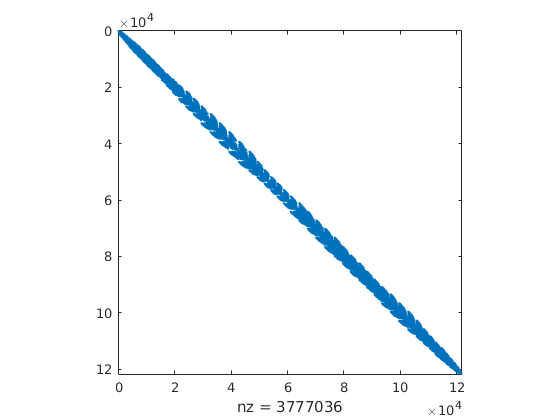
\includegraphics[width=0.7\linewidth]{../src/figure/ship}
\caption{Visualisation of the sparsity pattern of the \texttt{ship003}-matrix}
\label{fig:ship}
\end{figure}
\begin{table}
\centering
\begin{tabular}{|c|c|c|c|c|} \hline
  \#vectors & ilu level of fill & memory & time & relative error \\
   10  & 1 & \texttt{9.473 GB} & 61.5548s & 20.8122\\
   100 & 1 & \texttt{9.561 GB}  & 81.6827s & 1.15364 \\
   10  & 0 & \texttt{1.037 GB}  & 48.2886s & 91.2033 \\ 
   100 & 0 & \texttt{1.125 GB}  & 66.3984s & 3.18241 \\ \hline
\end{tabular}
\caption{Time, memory and accuracy test results of various GMRES computations, on the ship 003 matrix. The preconditioner's level of fill as well as the number of available vectors have been varied.}
\label{tab:shipGMRES}
\end{table}
Figure~\ref{fig:ship} shows the sparsity pattern of the \texttt{ship03} matrix. Results of iterative computations using the GMRES-algorithm are shown in table~\ref{tab:shipGMRES}. The results here are similar to what was observed earlier. Decreasing the level of fill or vector number leads to faster computation time and higher error. Convergence plots are given in Figure~\ref{fig:shipConvergence}. Interestingly the  GMRES algorithms only find the correct solution, if the methods have at least 100 vectors at their disposal. In contrast to the rajat matrix, which was experimented with earlier, the level of fill is not so important. Indicating, that both preconditioners are of similar quality. Unfortunately the matrix is too large for eigenvalue computations on the machine available, making further investigation impossible. The bicgstab algorithm does not converge, as the solution it computes is useless it's memory usage has not been measured. Again the direct method outperforms the iterative ones producing a solution with an error of $1.273*10^{-10}$ within $21.7s$ using \texttt{2.996 GB} of RAM.

\subsection{Fault639}
\begin{figure}
\centering
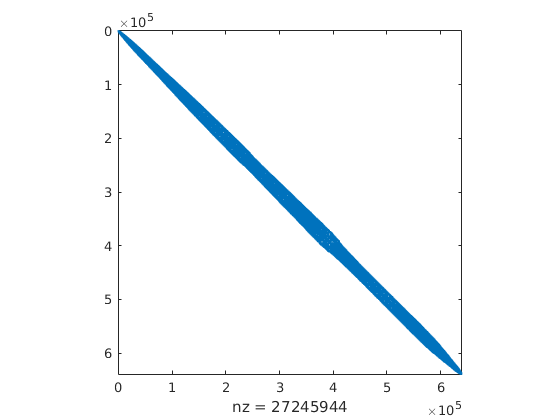
\includegraphics[width=0.7\linewidth]{../src/figure/Fault}
\caption{Visualisation of the sparsity pattern of the \texttt{fault639}-matrix}
\label{fig:fault}
\end{figure}
\begin{table}
\centering
\begin{tabular}{|c|c|c|c|c|} \hline
  \#vectors & ilu level of fill & memory & CPU time & relative error \\
   10  & 1  & ?? & 269.7s & 0.962255  \\
   100 & 1  & ?? & 465 s  & 0.82716  \\
   10  & 0  & \texttt{ 3.723 GB} & 181.4s & 0.892187  \\
   100 & 0  & \texttt{ 4.184 GB} & 357.1s & 0.0304293  \\ \hline
\end{tabular}
\caption{Memory requirements of GMRES when run on the fault matrix. }
\label{tab:FaultGMRES}
\end{table}
\begin{figure}
\centering
% This file was created by matlab2tikz.
% Minimal pgfplots version: 1.3
%
%The latest updates can be retrieved from
%  http://www.mathworks.com/matlabcentral/fileexchange/22022-matlab2tikz
%where you can also make suggestions and rate matlab2tikz.
%
\documentclass[tikz]{standalone}
\usepackage{pgfplots}
\usepackage{grffile}
\pgfplotsset{compat=newest}
\usetikzlibrary{plotmarks}
\usepackage{amsmath}

\begin{document}
\definecolor{mycolor1}{rgb}{0.00000,0.44700,0.74100}%
\definecolor{mycolor2}{rgb}{0.85000,0.32500,0.09800}%
\definecolor{mycolor3}{rgb}{0.92900,0.69400,0.12500}%
\definecolor{mycolor4}{rgb}{0.49400,0.18400,0.55600}%
\definecolor{mycolor5}{rgb}{0.46600,0.67400,0.18800}%
%
\begin{tikzpicture}

\begin{axis}[%
width=4.520833in,
height=3.565625in,
at={(0.758333in,0.48125in)},
scale only axis,
xmode=log,
xmin=1,
xmax=10000,
xminorticks=true,
xmajorgrids,
xminorgrids,
ymode=log,
ymin=1e-05,
ymax=1e+20,
yminorticks=true,
ymajorgrids,
yminorgrids,
legend style={legend cell align=left,align=left,draw=white!15!black}
]
\addplot [color=mycolor1,solid]
  table[row sep=crcr]{%
1	158.281\\
2	23.8594\\
3	18.6232\\
4	16.2258\\
5	16.117\\
6	12.7603\\
7	11.7169\\
8	11.4394\\
9	9.43246\\
10	9.27146\\
11	8.64885\\
12	8.40497\\
13	8.38794\\
14	8.38649\\
15	8.37539\\
16	8.3565\\
17	8.32316\\
18	8.30146\\
19	8.23249\\
20	8.11623\\
21	8.11623\\
22	8.11622\\
23	8.01244\\
24	7.98772\\
25	7.98137\\
26	7.97557\\
27	7.94458\\
28	7.92927\\
29	7.92025\\
30	7.91828\\
31	7.88764\\
32	7.88707\\
33	7.86357\\
34	7.85633\\
35	7.85484\\
36	7.83382\\
37	7.82379\\
38	7.80238\\
39	7.80209\\
40	7.75743\\
41	7.69096\\
42	7.68651\\
43	7.65238\\
44	7.58899\\
45	7.58879\\
46	7.57864\\
47	7.56985\\
48	7.54793\\
49	7.54174\\
50	7.54054\\
51	7.52068\\
52	7.51987\\
53	7.50806\\
54	7.50015\\
55	7.49978\\
56	7.49488\\
57	7.47834\\
58	7.46687\\
59	7.45544\\
60	7.45379\\
61	7.3803\\
62	7.36232\\
63	7.34367\\
64	7.31138\\
65	7.30496\\
66	7.30267\\
67	7.29162\\
68	7.27669\\
69	7.26503\\
70	7.26486\\
71	7.25313\\
72	7.24795\\
73	7.24633\\
74	7.23779\\
75	7.23599\\
76	7.23426\\
77	7.22463\\
78	7.2091\\
79	7.19757\\
80	7.19747\\
81	7.13752\\
82	7.08423\\
83	7.08194\\
84	7.0808\\
85	7.06682\\
86	7.05315\\
87	7.0531\\
88	7.04952\\
89	7.03633\\
90	7.03313\\
91	7.02901\\
92	7.02577\\
93	7.02482\\
94	7.01651\\
95	7.00687\\
96	7.00518\\
97	7.00293\\
98	6.98947\\
99	6.9803\\
100	6.9802\\
101	6.95146\\
102	6.9507\\
103	6.93368\\
104	6.92823\\
105	6.92818\\
106	6.90951\\
107	6.90166\\
108	6.90162\\
109	6.89377\\
110	6.88379\\
111	6.88162\\
112	6.87984\\
113	6.87417\\
114	6.86566\\
115	6.86215\\
116	6.85742\\
117	6.85003\\
118	6.8386\\
119	6.83819\\
120	6.82628\\
121	6.81347\\
122	6.80183\\
123	6.79023\\
124	6.7894\\
125	6.78868\\
126	6.77518\\
127	6.76781\\
128	6.76662\\
129	6.75714\\
130	6.74962\\
131	6.74784\\
132	6.7466\\
133	6.74073\\
134	6.73241\\
135	6.73005\\
136	6.72368\\
137	6.70849\\
138	6.70658\\
139	6.70522\\
140	6.69677\\
141	6.67842\\
142	6.66138\\
143	6.65278\\
144	6.65111\\
145	6.65039\\
146	6.64251\\
147	6.6321\\
148	6.62921\\
149	6.61871\\
150	6.61391\\
151	6.61254\\
152	6.6107\\
153	6.60388\\
154	6.59629\\
155	6.59422\\
156	6.58982\\
157	6.58055\\
158	6.57373\\
159	6.5734\\
160	6.56149\\
161	6.53979\\
162	6.52142\\
163	6.50894\\
164	6.50777\\
165	6.49997\\
166	6.49207\\
167	6.48711\\
168	6.48615\\
169	6.4794\\
170	6.47341\\
171	6.47173\\
172	6.47015\\
173	6.46541\\
174	6.45468\\
175	6.45369\\
176	6.45076\\
177	6.44519\\
178	6.43482\\
179	6.43447\\
180	6.42443\\
181	6.39712\\
182	6.37274\\
183	6.36136\\
184	6.36062\\
185	6.35917\\
186	6.34776\\
187	6.34134\\
188	6.33262\\
189	6.32903\\
190	6.32537\\
191	6.324\\
192	6.32303\\
193	6.32064\\
194	6.31774\\
195	6.3095\\
196	6.30836\\
197	6.30669\\
198	6.28679\\
199	6.28676\\
200	6.27702\\
201	6.24711\\
202	6.23036\\
203	6.21234\\
204	6.21046\\
205	6.21028\\
206	6.20115\\
207	6.19019\\
208	6.1901\\
209	6.18149\\
210	6.17836\\
211	6.1776\\
212	6.17674\\
213	6.17087\\
214	6.16178\\
215	6.16014\\
216	6.15659\\
217	6.15049\\
218	6.14036\\
219	6.13973\\
220	6.11998\\
221	6.09762\\
222	6.07596\\
223	6.05715\\
224	6.05614\\
225	6.04887\\
226	6.04265\\
227	6.03732\\
228	6.03713\\
229	6.02981\\
230	6.02407\\
231	6.02353\\
232	6.02316\\
233	6.02079\\
234	6.00919\\
235	6.00671\\
236	6.00552\\
237	5.98643\\
238	5.98202\\
239	5.9816\\
240	5.96897\\
241	5.93831\\
242	5.92084\\
243	5.90511\\
244	5.90033\\
245	5.89958\\
246	5.87536\\
247	5.87308\\
248	5.87301\\
249	5.86487\\
250	5.86172\\
251	5.86112\\
252	5.86036\\
253	5.85549\\
254	5.84912\\
255	5.84156\\
256	5.84124\\
257	5.82809\\
258	5.79709\\
259	5.79671\\
260	5.72038\\
261	5.71933\\
262	5.71817\\
263	5.6682\\
264	5.6536\\
265	5.6519\\
266	5.63136\\
267	5.60798\\
268	5.60413\\
269	5.59747\\
270	5.59415\\
271	5.59295\\
272	5.59242\\
273	5.59074\\
274	5.58559\\
275	5.56296\\
276	5.55795\\
277	5.55772\\
278	5.48034\\
279	5.3989\\
280	5.39309\\
281	5.01231\\
282	4.9983\\
283	4.82149\\
284	4.75711\\
285	4.72689\\
286	4.7084\\
287	4.64887\\
288	4.64069\\
289	4.64054\\
290	4.63047\\
291	4.6258\\
292	4.62439\\
293	4.62427\\
294	4.62241\\
295	4.6185\\
296	4.61817\\
297	4.61776\\
298	4.60985\\
299	4.60842\\
300	4.60747\\
301	4.60248\\
302	4.59859\\
303	4.59696\\
304	4.5963\\
305	4.5916\\
306	4.58439\\
307	4.58436\\
308	4.57817\\
309	4.57465\\
310	4.55445\\
311	4.54194\\
312	4.53348\\
313	4.52071\\
314	4.51547\\
315	4.51231\\
316	4.51207\\
317	4.51132\\
318	4.50442\\
319	4.50178\\
320	4.50177\\
321	4.49762\\
322	4.49709\\
323	4.49485\\
324	4.49473\\
325	4.49336\\
326	4.49104\\
327	4.48913\\
328	4.48848\\
329	4.4852\\
330	4.48346\\
331	4.48311\\
332	4.48258\\
333	4.48196\\
334	4.47908\\
335	4.47852\\
336	4.47745\\
337	4.47445\\
338	4.46235\\
339	4.45372\\
340	4.43645\\
341	4.41866\\
342	4.41853\\
343	4.41143\\
344	4.41032\\
345	4.41029\\
346	4.40918\\
347	4.40918\\
348	4.40285\\
349	4.40116\\
350	4.4002\\
351	4.39632\\
352	4.39553\\
353	4.39476\\
354	4.39422\\
355	4.39328\\
356	4.39308\\
357	4.39256\\
358	4.38588\\
359	4.38587\\
360	4.38481\\
361	4.3848\\
362	4.3848\\
363	4.38429\\
364	4.38426\\
365	4.38425\\
366	4.38422\\
367	4.38323\\
368	4.38195\\
369	4.37872\\
370	4.37837\\
371	4.3771\\
372	4.37675\\
373	4.3761\\
374	4.37452\\
375	4.37433\\
376	4.37424\\
377	4.3739\\
378	4.37289\\
379	4.37264\\
380	4.37262\\
381	4.37244\\
382	4.37243\\
383	4.37243\\
384	4.37238\\
385	4.37227\\
386	4.37225\\
387	4.37185\\
388	4.37138\\
389	4.36991\\
390	4.3699\\
391	4.3686\\
392	4.36824\\
393	4.36773\\
394	4.36707\\
395	4.36675\\
396	4.36665\\
397	4.36637\\
398	4.36555\\
399	4.36547\\
400	4.36543\\
401	4.36538\\
402	4.36538\\
403	4.36538\\
404	4.36535\\
405	4.36525\\
406	4.36518\\
407	4.3649\\
408	4.36388\\
409	4.36299\\
410	4.36292\\
411	4.36168\\
412	4.36144\\
413	4.36094\\
414	4.35999\\
415	4.35952\\
416	4.35929\\
417	4.35894\\
418	4.35869\\
419	4.35861\\
420	4.35846\\
421	4.35845\\
422	4.35845\\
423	4.35839\\
424	4.35838\\
425	4.35833\\
426	4.35822\\
427	4.35818\\
428	4.35802\\
429	4.35636\\
430	4.35635\\
431	4.35455\\
432	4.35403\\
433	4.35341\\
434	4.35143\\
435	4.35113\\
436	4.35112\\
437	4.35073\\
438	4.35052\\
439	4.35052\\
440	4.35044\\
441	4.35044\\
442	4.35044\\
443	4.35042\\
444	4.35041\\
445	4.35039\\
446	4.35032\\
447	4.35032\\
448	4.3502\\
449	4.34902\\
450	4.34888\\
451	4.34772\\
452	4.34712\\
453	4.34669\\
454	4.34614\\
455	4.34568\\
456	4.34567\\
457	4.34509\\
458	4.34494\\
459	4.34487\\
460	4.34478\\
461	4.34477\\
462	4.34476\\
463	4.34468\\
464	4.34468\\
465	4.34467\\
466	4.34465\\
467	4.34465\\
468	4.34459\\
469	4.34398\\
470	4.34348\\
471	4.34222\\
472	4.34149\\
473	4.34103\\
474	4.34056\\
475	4.34046\\
476	4.3403\\
477	4.33995\\
478	4.33988\\
479	4.33987\\
480	4.33965\\
481	4.33959\\
482	4.33959\\
483	4.33946\\
484	4.33942\\
485	4.3394\\
486	4.33932\\
487	4.33932\\
488	4.33927\\
489	4.33835\\
490	4.33788\\
491	4.33737\\
492	4.33699\\
493	4.3365\\
494	4.3359\\
495	4.33587\\
496	4.33572\\
497	4.3355\\
498	4.33549\\
499	4.3354\\
500	4.33529\\
501	4.3352\\
502	4.33519\\
503	4.33512\\
504	4.335\\
505	4.33499\\
506	4.33483\\
507	4.33483\\
508	4.33476\\
509	4.33364\\
510	4.33321\\
511	4.33263\\
512	4.33216\\
513	4.33166\\
514	4.33091\\
515	4.33091\\
516	4.33077\\
517	4.33046\\
518	4.33045\\
519	4.33029\\
520	4.33027\\
521	4.33018\\
522	4.33015\\
523	4.33011\\
524	4.32998\\
525	4.32998\\
526	4.32975\\
527	4.32974\\
528	4.32963\\
529	4.32806\\
530	4.32769\\
531	4.32687\\
532	4.32613\\
533	4.32569\\
534	4.32451\\
535	4.32451\\
536	4.32437\\
537	4.32389\\
538	4.32374\\
539	4.32368\\
540	4.32368\\
541	4.32323\\
542	4.32293\\
543	4.32289\\
544	4.32277\\
545	4.32262\\
546	4.32259\\
547	4.32235\\
548	4.32232\\
549	4.32033\\
550	4.31968\\
551	4.3188\\
552	4.31796\\
553	4.31736\\
554	4.31609\\
555	4.31605\\
556	4.3157\\
557	4.31549\\
558	4.31536\\
559	4.31521\\
560	4.31517\\
561	4.31481\\
562	4.31454\\
563	4.31448\\
564	4.31438\\
565	4.31432\\
566	4.31429\\
567	4.31412\\
568	4.31401\\
569	4.31083\\
570	4.31038\\
571	4.30839\\
572	4.30631\\
573	4.30595\\
574	4.30307\\
575	4.30285\\
576	4.30244\\
577	4.30177\\
578	4.30177\\
579	4.30135\\
580	4.30067\\
581	4.30056\\
582	4.30045\\
583	4.29999\\
584	4.29977\\
585	4.29977\\
586	4.29865\\
587	4.29752\\
588	4.29579\\
589	4.29457\\
590	4.29195\\
591	4.29092\\
592	4.28986\\
593	4.28786\\
594	4.28678\\
595	4.28661\\
596	4.28545\\
597	4.28431\\
598	4.28423\\
599	4.28358\\
600	4.28338\\
601	4.28335\\
602	4.28334\\
603	4.28297\\
604	4.28289\\
605	4.28287\\
606	4.28223\\
607	4.28043\\
608	4.26795\\
609	4.26782\\
610	4.23776\\
611	4.22419\\
612	4.21712\\
613	4.19435\\
614	4.1858\\
615	4.17611\\
616	4.16575\\
617	4.16312\\
618	4.16158\\
619	4.16158\\
620	4.16118\\
621	4.16084\\
622	4.16082\\
623	4.16073\\
624	4.16073\\
625	4.16069\\
626	4.16044\\
627	4.16041\\
628	4.16039\\
629	4.15835\\
630	4.12829\\
631	4.12729\\
632	4.12617\\
633	4.10496\\
634	4.09673\\
635	4.09486\\
636	4.09441\\
637	4.09432\\
638	4.09416\\
639	4.0939\\
640	4.09385\\
641	4.09358\\
642	4.09352\\
643	4.09351\\
644	4.09349\\
645	4.09343\\
646	4.09319\\
647	4.09306\\
648	4.09295\\
649	4.07834\\
650	4.05589\\
651	4.05406\\
652	4.05206\\
653	4.0339\\
654	4.01964\\
655	4.01769\\
656	4.01737\\
657	4.01569\\
658	4.01568\\
659	4.01561\\
660	4.0155\\
661	4.0155\\
662	4.0155\\
663	4.01543\\
664	4.01542\\
665	4.01535\\
666	4.01419\\
667	4.01218\\
668	4.00909\\
669	4.00736\\
670	3.92453\\
671	3.8235\\
672	3.79723\\
673	3.78886\\
674	3.7495\\
675	3.74729\\
676	3.7419\\
677	3.73385\\
678	3.73331\\
679	3.71943\\
680	3.71893\\
681	3.706\\
682	3.69374\\
683	3.69356\\
684	3.68756\\
685	3.68678\\
686	3.68659\\
687	3.68636\\
688	3.68635\\
689	3.68323\\
690	3.68274\\
691	3.67872\\
692	3.67596\\
693	3.67561\\
694	3.67486\\
695	3.67455\\
696	3.67437\\
697	3.67437\\
698	3.67437\\
699	3.67411\\
700	3.67408\\
701	3.67408\\
702	3.67407\\
703	3.67407\\
704	3.67389\\
705	3.67389\\
706	3.67386\\
707	3.67384\\
708	3.67363\\
709	3.67329\\
710	3.67195\\
711	3.66987\\
712	3.66846\\
713	3.66845\\
714	3.66716\\
715	3.66716\\
716	3.66701\\
717	3.66651\\
718	3.66645\\
719	3.66641\\
720	3.66626\\
721	3.66615\\
722	3.66613\\
723	3.66612\\
724	3.66608\\
725	3.66607\\
726	3.66604\\
727	3.66602\\
728	3.66582\\
729	3.6655\\
730	3.664\\
731	3.66041\\
732	3.65768\\
733	3.65768\\
734	3.65589\\
735	3.65588\\
736	3.65559\\
737	3.65513\\
738	3.65513\\
739	3.65506\\
740	3.65496\\
741	3.6549\\
742	3.65489\\
743	3.65489\\
744	3.65487\\
745	3.65487\\
746	3.65481\\
747	3.65481\\
748	3.65462\\
749	3.65417\\
750	3.65359\\
751	3.63599\\
752	3.62939\\
753	3.6293\\
754	3.62576\\
755	3.62539\\
756	3.62524\\
757	3.62483\\
758	3.62456\\
759	3.62441\\
760	3.62425\\
761	3.62424\\
762	3.62424\\
763	3.62423\\
764	3.62415\\
765	3.62413\\
766	3.62407\\
767	3.62407\\
768	3.62395\\
769	3.6238\\
770	3.62316\\
771	3.6221\\
772	3.62165\\
773	3.62161\\
774	3.6212\\
775	3.62115\\
776	3.62102\\
777	3.62066\\
778	3.62027\\
779	3.62025\\
780	3.62016\\
781	3.62011\\
782	3.6201\\
783	3.6201\\
784	3.62008\\
785	3.62008\\
786	3.62004\\
787	3.62004\\
788	3.61982\\
789	3.61966\\
790	3.6191\\
791	3.61578\\
792	3.6134\\
793	3.61336\\
794	3.61305\\
795	3.61274\\
796	3.61274\\
797	3.61242\\
798	3.61197\\
799	3.61192\\
800	3.61186\\
801	3.61173\\
802	3.61172\\
803	3.61172\\
804	3.61172\\
805	3.61172\\
806	3.61171\\
807	3.6117\\
808	3.61119\\
809	3.61114\\
810	3.60992\\
811	3.59714\\
812	3.58837\\
813	3.58766\\
814	3.58478\\
815	3.58424\\
816	3.58422\\
817	3.58318\\
818	3.58264\\
819	3.58264\\
820	3.58264\\
821	3.58204\\
822	3.58204\\
823	3.58203\\
824	3.58202\\
825	3.58202\\
826	3.58191\\
827	3.58191\\
828	3.58179\\
829	3.58113\\
830	3.58113\\
831	3.57661\\
832	3.57379\\
833	3.57379\\
834	3.57298\\
835	3.57275\\
836	3.57273\\
837	3.57243\\
838	3.57213\\
839	3.57202\\
840	3.57194\\
841	3.57177\\
842	3.57176\\
843	3.57176\\
844	3.57176\\
845	3.57176\\
846	3.57176\\
847	3.57175\\
848	3.57153\\
849	3.57116\\
850	3.57054\\
851	3.56755\\
852	3.56513\\
853	3.56512\\
854	3.56379\\
855	3.5635\\
856	3.56341\\
857	3.5631\\
858	3.56283\\
859	3.56271\\
860	3.56264\\
861	3.56252\\
862	3.56251\\
863	3.56251\\
864	3.56251\\
865	3.56251\\
866	3.5625\\
867	3.56249\\
868	3.56225\\
869	3.56206\\
870	3.56198\\
871	3.56098\\
872	3.56034\\
873	3.56028\\
874	3.56013\\
875	3.56003\\
876	3.56\\
877	3.55977\\
878	3.55938\\
879	3.55918\\
880	3.55881\\
881	3.55868\\
882	3.55867\\
883	3.55866\\
884	3.55851\\
885	3.5585\\
886	3.55838\\
887	3.55838\\
888	3.55817\\
889	3.55796\\
890	3.5579\\
891	3.55721\\
892	3.55687\\
893	3.55681\\
894	3.55672\\
895	3.55668\\
896	3.55668\\
897	3.55651\\
898	3.55616\\
899	3.55596\\
900	3.55556\\
901	3.55306\\
902	3.55172\\
903	3.55161\\
904	3.55099\\
905	3.55049\\
906	3.55025\\
907	3.55013\\
908	3.5501\\
909	3.5495\\
910	3.54948\\
911	3.54892\\
912	3.54879\\
913	3.54877\\
914	3.54867\\
915	3.54867\\
916	3.54864\\
917	3.54853\\
918	3.54836\\
919	3.54828\\
920	3.54807\\
921	3.54803\\
922	3.54802\\
923	3.54801\\
924	3.54791\\
925	3.54791\\
926	3.5478\\
927	3.5478\\
928	3.5477\\
929	3.54742\\
930	3.54711\\
931	3.54505\\
932	3.54404\\
933	3.54403\\
934	3.54361\\
935	3.54328\\
936	3.54323\\
937	3.54308\\
938	3.54301\\
939	3.54288\\
940	3.54287\\
941	3.54281\\
942	3.54281\\
943	3.54281\\
944	3.5428\\
945	3.5428\\
946	3.5428\\
947	3.5428\\
948	3.54266\\
949	3.54253\\
950	3.54221\\
951	3.53972\\
952	3.53856\\
953	3.53856\\
954	3.53719\\
955	3.53702\\
956	3.5369\\
957	3.53653\\
958	3.53622\\
959	3.53616\\
960	3.53614\\
961	3.53606\\
962	3.53605\\
963	3.53605\\
964	3.53604\\
965	3.53604\\
966	3.53603\\
967	3.53599\\
968	3.53592\\
969	3.53584\\
970	3.53578\\
971	3.53518\\
972	3.53498\\
973	3.53496\\
974	3.53465\\
975	3.53465\\
976	3.53458\\
977	3.53445\\
978	3.53419\\
979	3.53399\\
980	3.53371\\
981	3.53353\\
982	3.53351\\
983	3.53351\\
984	3.53328\\
985	3.53327\\
986	3.53317\\
987	3.53309\\
988	3.53302\\
989	3.53296\\
990	3.53292\\
991	3.53248\\
992	3.53237\\
993	3.53235\\
994	3.53219\\
995	3.53216\\
996	3.5321\\
997	3.53201\\
998	3.53183\\
999	3.53165\\
1000	3.53129\\
1001	3.52811\\
1002	3.5265\\
1003	3.52648\\
1004	3.52517\\
1005	3.52437\\
1006	3.52398\\
1007	3.52384\\
1008	3.52382\\
1009	3.52347\\
1010	3.52347\\
1011	3.52334\\
1012	3.52333\\
1013	3.52332\\
1014	3.52328\\
1015	3.52328\\
1016	3.52325\\
1017	3.52322\\
1018	3.52319\\
1019	3.52303\\
1020	3.5229\\
1021	3.52277\\
1022	3.52275\\
1023	3.52275\\
1024	3.52261\\
1025	3.52255\\
1026	3.52243\\
1027	3.5224\\
1028	3.5224\\
1029	3.522\\
1030	3.52196\\
1031	3.52116\\
1032	3.52098\\
1033	3.52097\\
1034	3.52065\\
1035	3.52062\\
1036	3.52051\\
1037	3.52045\\
1038	3.52044\\
1039	3.52023\\
1040	3.5202\\
1041	3.5202\\
1042	3.5202\\
1043	3.52019\\
1044	3.52013\\
1045	3.52013\\
1046	3.52006\\
1047	3.52006\\
1048	3.52001\\
1049	3.51974\\
1050	3.51966\\
1051	3.51771\\
1052	3.51724\\
1053	3.51724\\
1054	3.51584\\
1055	3.51584\\
1056	3.5154\\
1057	3.51523\\
1058	3.51513\\
1059	3.515\\
1060	3.5149\\
1061	3.51489\\
1062	3.51489\\
1063	3.51489\\
1064	3.51482\\
1065	3.51482\\
1066	3.5148\\
1067	3.51479\\
1068	3.51476\\
1069	3.51461\\
1070	3.51461\\
1071	3.5144\\
1072	3.51437\\
1073	3.51437\\
1074	3.5142\\
1075	3.5142\\
1076	3.51408\\
1077	3.51402\\
1078	3.51397\\
1079	3.51365\\
1080	3.51333\\
1081	3.51319\\
1082	3.51317\\
1083	3.51316\\
1084	3.51286\\
1085	3.51286\\
1086	3.51279\\
1087	3.51278\\
1088	3.51274\\
1089	3.51262\\
1090	3.51262\\
1091	3.5125\\
1092	3.51248\\
1093	3.51248\\
1094	3.5124\\
1095	3.5124\\
1096	3.51233\\
1097	3.5123\\
1098	3.51228\\
1099	3.512\\
1100	3.51147\\
1101	3.50697\\
1102	3.50432\\
1103	3.50428\\
1104	3.5026\\
1105	3.50145\\
1106	3.50113\\
1107	3.50098\\
1108	3.50095\\
1109	3.50062\\
1110	3.50061\\
1111	3.5006\\
1112	3.5006\\
1113	3.5006\\
1114	3.50058\\
1115	3.50058\\
1116	3.50056\\
1117	3.50055\\
1118	3.50054\\
1119	3.50034\\
1120	3.50006\\
1121	3.49991\\
1122	3.49988\\
1123	3.49986\\
1124	3.49956\\
1125	3.49948\\
1126	3.49938\\
1127	3.49935\\
1128	3.49935\\
1129	3.49888\\
1130	3.49888\\
1131	3.49848\\
1132	3.49843\\
1133	3.49843\\
1134	3.49826\\
1135	3.49823\\
1136	3.4981\\
1137	3.49807\\
1138	3.49807\\
1139	3.49783\\
1140	3.49773\\
1141	3.49771\\
1142	3.49771\\
1143	3.4977\\
1144	3.49755\\
1145	3.49754\\
1146	3.49749\\
1147	3.49747\\
1148	3.49742\\
1149	3.49701\\
1150	3.49701\\
1151	3.49258\\
1152	3.4911\\
1153	3.49109\\
1154	3.48974\\
1155	3.48881\\
1156	3.48859\\
1157	3.48812\\
1158	3.48774\\
1159	3.48747\\
1160	3.48731\\
1161	3.48729\\
1162	3.48728\\
1163	3.48727\\
1164	3.48713\\
1165	3.48712\\
1166	3.48708\\
1167	3.48707\\
1168	3.48703\\
1169	3.48671\\
1170	3.48671\\
1171	3.48617\\
1172	3.48607\\
1173	3.48607\\
1174	3.48558\\
1175	3.48558\\
1176	3.48531\\
1177	3.48521\\
1178	3.48517\\
1179	3.4848\\
1180	3.4846\\
1181	3.48457\\
1182	3.48457\\
1183	3.48455\\
1184	3.48434\\
1185	3.48433\\
1186	3.48431\\
1187	3.48431\\
1188	3.48426\\
1189	3.4841\\
1190	3.48407\\
1191	3.48398\\
1192	3.48397\\
1193	3.48397\\
1194	3.48387\\
1195	3.48387\\
1196	3.48378\\
1197	3.48375\\
1198	3.48375\\
1199	3.48315\\
1200	3.48204\\
1201	3.48015\\
1202	3.47956\\
1203	3.47951\\
1204	3.47768\\
1205	3.47768\\
1206	3.47753\\
1207	3.47752\\
1208	3.47747\\
1209	3.47728\\
1210	3.47727\\
1211	3.47723\\
1212	3.47722\\
1213	3.47722\\
1214	3.47719\\
1215	3.47718\\
1216	3.47713\\
1217	3.47711\\
1218	3.47711\\
1219	3.4768\\
1220	3.47627\\
1221	3.47626\\
1222	3.47626\\
1223	3.47619\\
1224	3.47554\\
1225	3.47554\\
1226	3.47537\\
1227	3.47534\\
1228	3.4753\\
1229	3.47493\\
1230	3.47492\\
1231	3.47485\\
1232	3.47485\\
1233	3.47485\\
1234	3.47479\\
1235	3.47479\\
1236	3.47473\\
1237	3.47472\\
1238	3.47472\\
1239	3.47454\\
1240	3.47424\\
1241	3.47413\\
1242	3.47412\\
1243	3.47403\\
1244	3.47374\\
1245	3.47373\\
1246	3.4737\\
1247	3.4737\\
1248	3.47366\\
1249	3.47323\\
1250	3.47321\\
1251	3.46658\\
1252	3.46374\\
1253	3.46374\\
1254	3.46156\\
1255	3.46136\\
1256	3.46097\\
1257	3.4609\\
1258	3.4609\\
1259	3.46062\\
1260	3.46036\\
1261	3.46017\\
1262	3.46014\\
1263	3.46005\\
1264	3.45977\\
1265	3.45974\\
1266	3.45973\\
1267	3.45973\\
1268	3.45969\\
1269	3.45939\\
1270	3.45935\\
1271	3.45898\\
1272	3.45892\\
1273	3.45892\\
1274	3.45866\\
1275	3.4586\\
1276	3.45829\\
1277	3.4582\\
1278	3.45819\\
1279	3.45773\\
1280	3.45733\\
1281	3.45717\\
1282	3.45714\\
1283	3.457\\
1284	3.45663\\
1285	3.45659\\
1286	3.45659\\
1287	3.45658\\
1288	3.45654\\
1289	3.4563\\
1290	3.45626\\
1291	3.45619\\
1292	3.45618\\
1293	3.45618\\
1294	3.45613\\
1295	3.45612\\
1296	3.45601\\
1297	3.45598\\
1298	3.45598\\
1299	3.45487\\
1300	3.45293\\
1301	3.45242\\
1302	3.45219\\
1303	3.45156\\
1304	3.45019\\
1305	3.44977\\
1306	3.44972\\
1307	3.4497\\
1308	3.44967\\
1309	3.44929\\
1310	3.44928\\
1311	3.44927\\
1312	3.44927\\
1313	3.44927\\
1314	3.44926\\
1315	3.44926\\
1316	3.4492\\
1317	3.44919\\
1318	3.44919\\
1319	3.44843\\
1320	3.44708\\
1321	3.44708\\
1322	3.44708\\
1323	3.44657\\
1324	3.44526\\
1325	3.44523\\
1326	3.44513\\
1327	3.44506\\
1328	3.44505\\
1329	3.44441\\
1330	3.4444\\
1331	3.44437\\
1332	3.44437\\
1333	3.44437\\
1334	3.44434\\
1335	3.44434\\
1336	3.44428\\
1337	3.44428\\
1338	3.44428\\
1339	3.44402\\
1340	3.4429\\
1341	3.44266\\
1342	3.44257\\
1343	3.44199\\
1344	3.44144\\
1345	3.44139\\
1346	3.44139\\
1347	3.44138\\
1348	3.44135\\
1349	3.4408\\
1350	3.44074\\
1351	3.43843\\
1352	3.43791\\
1353	3.43791\\
1354	3.43722\\
1355	3.43689\\
1356	3.43659\\
1357	3.43653\\
1358	3.43653\\
1359	3.4363\\
1360	3.43563\\
1361	3.43509\\
1362	3.43496\\
1363	3.43459\\
1364	3.4341\\
1365	3.43403\\
1366	3.43402\\
1367	3.43402\\
1368	3.43398\\
1369	3.43357\\
1370	3.43351\\
1371	3.43323\\
1372	3.4332\\
1373	3.4332\\
1374	3.43293\\
1375	3.43293\\
1376	3.43263\\
1377	3.43253\\
1378	3.43253\\
1379	3.43206\\
1380	3.43141\\
1381	3.43085\\
1382	3.43073\\
1383	3.43041\\
1384	3.42981\\
1385	3.42976\\
1386	3.42975\\
1387	3.42974\\
1388	3.42971\\
1389	3.42935\\
1390	3.42924\\
1391	3.42921\\
1392	3.4292\\
1393	3.4292\\
1394	3.42917\\
1395	3.42917\\
1396	3.42907\\
1397	3.42903\\
1398	3.42902\\
1399	3.42772\\
1400	3.4257\\
1401	3.42568\\
1402	3.42568\\
1403	3.42508\\
1404	3.42355\\
1405	3.42338\\
1406	3.42333\\
1407	3.42327\\
1408	3.42327\\
1409	3.42282\\
1410	3.4228\\
1411	3.42274\\
1412	3.42274\\
1413	3.42274\\
1414	3.42274\\
1415	3.42274\\
1416	3.42273\\
1417	3.42273\\
1418	3.42257\\
1419	3.42084\\
1420	3.41892\\
1421	3.41871\\
1422	3.41865\\
1423	3.41848\\
1424	3.41598\\
1425	3.41594\\
1426	3.41561\\
1427	3.41548\\
1428	3.41548\\
1429	3.41497\\
1430	3.4149\\
1431	3.4148\\
1432	3.4148\\
1433	3.4148\\
1434	3.4148\\
1435	3.4148\\
1436	3.41479\\
1437	3.41479\\
1438	3.4146\\
1439	3.41261\\
1440	3.40985\\
1441	3.40889\\
1442	3.40855\\
1443	3.40836\\
1444	3.40464\\
1445	3.40433\\
1446	3.40398\\
1447	3.40373\\
1448	3.40369\\
1449	3.40306\\
1450	3.40302\\
1451	3.40295\\
1452	3.40295\\
1453	3.40295\\
1454	3.40295\\
1455	3.40295\\
1456	3.40291\\
1457	3.40256\\
1458	3.40214\\
1459	3.4007\\
1460	3.39763\\
1461	3.39583\\
1462	3.39487\\
1463	3.39405\\
1464	3.39072\\
1465	3.39019\\
1466	3.39017\\
1467	3.38993\\
1468	3.38984\\
1469	3.38919\\
1470	3.38914\\
1471	3.389\\
1472	3.38899\\
1473	3.38899\\
1474	3.38899\\
1475	3.38899\\
1476	3.38899\\
1477	3.38898\\
1478	3.38834\\
1479	3.38406\\
1480	3.37891\\
1481	3.33073\\
1482	3.30193\\
1483	3.30144\\
1484	3.28419\\
1485	3.28161\\
1486	3.28144\\
1487	3.28085\\
1488	3.28044\\
1489	3.27949\\
1490	3.27915\\
1491	3.27885\\
1492	3.27884\\
1493	3.27884\\
1494	3.27884\\
1495	3.27884\\
1496	3.27883\\
1497	3.27881\\
1498	3.27857\\
1499	3.2781\\
1500	3.27717\\
1501	3.27715\\
1502	3.27714\\
1503	3.27701\\
1504	3.27634\\
1505	3.27609\\
1506	3.27601\\
1507	3.27596\\
1508	3.2759\\
1509	3.27521\\
1510	3.27499\\
1511	3.27497\\
};
\addlegendentry{gmres(0,10)};

\addplot [color=mycolor2,solid]
  table[row sep=crcr]{%
1	158.281\\
2	23.8594\\
3	18.6232\\
4	16.2258\\
5	16.117\\
6	12.7603\\
7	11.7169\\
8	11.4394\\
9	9.43246\\
10	9.27146\\
11	8.64885\\
12	8.27408\\
13	8.26368\\
14	8.15379\\
15	8.11982\\
16	8.09238\\
17	7.85197\\
18	7.11355\\
19	6.93239\\
20	6.91851\\
21	6.35594\\
22	6.0228\\
23	5.83695\\
24	5.82005\\
25	5.67926\\
26	5.37143\\
27	5.1927\\
28	5.19208\\
29	5.07355\\
30	4.79545\\
31	4.51105\\
32	4.46989\\
33	4.45901\\
34	4.20466\\
35	3.98747\\
36	3.75868\\
37	3.68744\\
38	3.64785\\
39	3.63353\\
40	3.55275\\
41	3.4075\\
42	3.2185\\
43	3.06355\\
44	2.90564\\
45	2.80552\\
46	2.7523\\
47	2.74298\\
48	2.71856\\
49	2.65146\\
50	2.57515\\
51	2.50179\\
52	2.47418\\
53	2.45248\\
54	2.44394\\
55	2.35497\\
56	2.30704\\
57	2.2311\\
58	2.17634\\
59	2.16198\\
60	2.10188\\
61	1.99549\\
62	1.86452\\
63	1.74251\\
64	1.61664\\
65	1.50246\\
66	1.41685\\
67	1.32057\\
68	1.27449\\
69	1.24283\\
70	1.23977\\
71	1.23634\\
72	1.19819\\
73	1.15607\\
74	1.07298\\
75	1.00213\\
76	0.951295\\
77	0.887057\\
78	0.850821\\
79	0.820187\\
80	0.793464\\
81	0.772473\\
82	0.754911\\
83	0.746227\\
84	0.743901\\
85	0.743688\\
86	0.737241\\
87	0.72546\\
88	0.70592\\
89	0.686706\\
90	0.673337\\
91	0.65583\\
92	0.641634\\
93	0.626567\\
94	0.610953\\
95	0.596981\\
96	0.582654\\
97	0.5706\\
98	0.557531\\
99	0.542821\\
100	0.532235\\
101	0.522722\\
102	0.520714\\
103	0.519783\\
104	0.518797\\
105	0.518196\\
106	0.518196\\
107	0.517949\\
108	0.517255\\
109	0.517019\\
110	0.516484\\
111	0.514891\\
112	0.514869\\
113	0.513544\\
114	0.5131\\
115	0.51308\\
116	0.511612\\
117	0.510332\\
118	0.51033\\
119	0.508519\\
120	0.508279\\
121	0.507615\\
122	0.506903\\
123	0.506895\\
124	0.50494\\
125	0.502889\\
126	0.502097\\
127	0.502087\\
128	0.501247\\
129	0.500066\\
130	0.499968\\
131	0.499594\\
132	0.498089\\
133	0.496756\\
134	0.496196\\
135	0.495929\\
136	0.495697\\
137	0.494835\\
138	0.4933\\
139	0.492127\\
140	0.491447\\
141	0.491431\\
142	0.491193\\
143	0.490322\\
144	0.488399\\
145	0.486138\\
146	0.484965\\
147	0.48387\\
148	0.483842\\
149	0.483595\\
150	0.481617\\
151	0.479572\\
152	0.478145\\
153	0.47664\\
154	0.47644\\
155	0.476227\\
156	0.47464\\
157	0.472182\\
158	0.468639\\
159	0.465027\\
160	0.461742\\
161	0.45797\\
162	0.454609\\
163	0.45248\\
164	0.450634\\
165	0.449867\\
166	0.449728\\
167	0.449674\\
168	0.449075\\
169	0.447654\\
170	0.44509\\
171	0.442575\\
172	0.4398\\
173	0.436906\\
174	0.434633\\
175	0.431437\\
176	0.428337\\
177	0.424971\\
178	0.421074\\
179	0.416373\\
180	0.41144\\
181	0.405374\\
182	0.398772\\
183	0.392245\\
184	0.385738\\
185	0.380681\\
186	0.375894\\
187	0.370316\\
188	0.365402\\
189	0.36116\\
190	0.357028\\
191	0.354145\\
192	0.350829\\
193	0.347097\\
194	0.343173\\
195	0.338642\\
196	0.334439\\
197	0.329602\\
198	0.324047\\
199	0.318234\\
200	0.311914\\
201	0.306167\\
202	0.306031\\
203	0.305292\\
204	0.304895\\
205	0.304801\\
206	0.304532\\
207	0.303629\\
208	0.303151\\
209	0.302759\\
210	0.302466\\
211	0.302455\\
212	0.302195\\
213	0.301298\\
214	0.301297\\
215	0.30052\\
216	0.299812\\
217	0.299441\\
218	0.299356\\
219	0.298931\\
220	0.298927\\
221	0.29841\\
222	0.29793\\
223	0.297923\\
224	0.297587\\
225	0.297409\\
226	0.297358\\
227	0.296777\\
228	0.296002\\
229	0.295668\\
230	0.295653\\
231	0.294631\\
232	0.293805\\
233	0.293143\\
234	0.292953\\
235	0.292939\\
236	0.292861\\
237	0.292416\\
238	0.291846\\
239	0.291333\\
240	0.29124\\
241	0.291126\\
242	0.290608\\
243	0.289344\\
244	0.288219\\
245	0.287045\\
246	0.286047\\
247	0.285793\\
248	0.285758\\
249	0.285688\\
250	0.285114\\
251	0.284556\\
252	0.284056\\
253	0.283895\\
254	0.28373\\
255	0.28311\\
256	0.281893\\
257	0.2804\\
258	0.279157\\
259	0.278057\\
260	0.277337\\
261	0.277104\\
262	0.277102\\
263	0.276952\\
264	0.276326\\
265	0.27543\\
266	0.274261\\
267	0.273241\\
268	0.272055\\
269	0.271095\\
270	0.270143\\
271	0.269092\\
272	0.267974\\
273	0.267124\\
274	0.266237\\
275	0.265498\\
276	0.264934\\
277	0.264558\\
278	0.264314\\
279	0.264195\\
280	0.264167\\
281	0.264164\\
282	0.264152\\
283	0.264118\\
284	0.264048\\
285	0.263913\\
286	0.263708\\
287	0.263416\\
288	0.262962\\
289	0.262356\\
290	0.261574\\
291	0.260676\\
292	0.259361\\
293	0.257765\\
294	0.255095\\
295	0.251381\\
296	0.247441\\
297	0.243241\\
298	0.238774\\
299	0.233296\\
300	0.227409\\
301	0.222223\\
302	0.221997\\
303	0.220757\\
304	0.220509\\
305	0.220508\\
306	0.219972\\
307	0.219244\\
308	0.219042\\
309	0.218407\\
310	0.218157\\
311	0.218111\\
312	0.217631\\
313	0.216939\\
314	0.216884\\
315	0.215941\\
316	0.215306\\
317	0.215295\\
318	0.214644\\
319	0.213996\\
320	0.213803\\
321	0.212718\\
322	0.21205\\
323	0.211973\\
324	0.211261\\
325	0.211162\\
326	0.210805\\
327	0.210197\\
328	0.210181\\
329	0.209998\\
330	0.20934\\
331	0.207907\\
332	0.207232\\
333	0.207049\\
334	0.207015\\
335	0.206737\\
336	0.205973\\
337	0.205388\\
338	0.204833\\
339	0.204708\\
340	0.204708\\
341	0.204512\\
342	0.204128\\
343	0.203102\\
344	0.202222\\
345	0.201641\\
346	0.201119\\
347	0.2011\\
348	0.201058\\
349	0.200739\\
350	0.200076\\
351	0.199333\\
352	0.198931\\
353	0.198726\\
354	0.198725\\
355	0.19847\\
356	0.197734\\
357	0.196553\\
358	0.195254\\
359	0.194104\\
360	0.193362\\
361	0.193072\\
362	0.193058\\
363	0.192989\\
364	0.192503\\
365	0.191752\\
366	0.190804\\
367	0.189713\\
368	0.188892\\
369	0.1882\\
370	0.187663\\
371	0.187216\\
372	0.186869\\
373	0.18663\\
374	0.186466\\
375	0.186384\\
376	0.186361\\
377	0.186359\\
378	0.186342\\
379	0.186276\\
380	0.186156\\
381	0.185902\\
382	0.18558\\
383	0.185218\\
384	0.184687\\
385	0.183935\\
386	0.183152\\
387	0.182114\\
388	0.18089\\
389	0.179659\\
390	0.178509\\
391	0.177429\\
392	0.17622\\
393	0.174975\\
394	0.173614\\
395	0.171878\\
396	0.170213\\
397	0.168796\\
398	0.166948\\
399	0.165251\\
400	0.162907\\
401	0.160524\\
402	0.16046\\
403	0.160158\\
404	0.159907\\
405	0.159764\\
406	0.159746\\
407	0.159355\\
408	0.15895\\
409	0.158881\\
410	0.158767\\
411	0.158763\\
412	0.158646\\
413	0.158245\\
414	0.158244\\
415	0.157804\\
416	0.157501\\
417	0.157475\\
418	0.157344\\
419	0.157111\\
420	0.157107\\
421	0.156914\\
422	0.156715\\
423	0.156713\\
424	0.156526\\
425	0.156479\\
426	0.156435\\
427	0.156238\\
428	0.156125\\
429	0.156122\\
430	0.155971\\
431	0.155488\\
432	0.155263\\
433	0.155122\\
434	0.155115\\
435	0.155088\\
436	0.15495\\
437	0.154705\\
438	0.154464\\
439	0.154325\\
440	0.154325\\
441	0.154182\\
442	0.153684\\
443	0.152964\\
444	0.152356\\
445	0.151825\\
446	0.151519\\
447	0.151507\\
448	0.151495\\
449	0.151276\\
450	0.150906\\
451	0.150618\\
452	0.150512\\
453	0.150435\\
454	0.15011\\
455	0.149517\\
456	0.148743\\
457	0.147933\\
458	0.147266\\
459	0.146606\\
460	0.146163\\
461	0.146019\\
462	0.146011\\
463	0.145937\\
464	0.145627\\
465	0.145123\\
466	0.144365\\
467	0.143649\\
468	0.14299\\
469	0.142453\\
470	0.14197\\
471	0.141421\\
472	0.140856\\
473	0.140414\\
474	0.139962\\
475	0.139529\\
476	0.139154\\
477	0.138841\\
478	0.138615\\
479	0.138497\\
480	0.138419\\
481	0.138392\\
482	0.138389\\
483	0.138389\\
484	0.138387\\
485	0.138363\\
486	0.138336\\
487	0.138278\\
488	0.138135\\
489	0.137974\\
490	0.137718\\
491	0.137438\\
492	0.137022\\
493	0.136477\\
494	0.135706\\
495	0.134623\\
496	0.133382\\
497	0.131826\\
498	0.130313\\
499	0.127943\\
500	0.125755\\
501	0.123996\\
502	0.12396\\
503	0.123647\\
504	0.123546\\
505	0.12354\\
506	0.123248\\
507	0.122934\\
508	0.122513\\
509	0.122447\\
510	0.122337\\
511	0.122321\\
512	0.122228\\
513	0.121844\\
514	0.121827\\
515	0.12145\\
516	0.121016\\
517	0.120795\\
518	0.120787\\
519	0.120442\\
520	0.120411\\
521	0.120206\\
522	0.120072\\
523	0.119897\\
524	0.119445\\
525	0.119359\\
526	0.119303\\
527	0.119013\\
528	0.118972\\
529	0.118925\\
530	0.11868\\
531	0.118124\\
532	0.117808\\
533	0.117679\\
534	0.117673\\
535	0.117565\\
536	0.117244\\
537	0.116923\\
538	0.116533\\
539	0.116442\\
540	0.116433\\
541	0.116422\\
542	0.116377\\
543	0.11614\\
544	0.115872\\
545	0.115724\\
546	0.115652\\
547	0.115638\\
548	0.115556\\
549	0.115326\\
550	0.115034\\
551	0.114762\\
552	0.114619\\
553	0.114549\\
554	0.114547\\
555	0.114431\\
556	0.11413\\
557	0.113702\\
558	0.113205\\
559	0.112862\\
560	0.112707\\
561	0.11267\\
562	0.112662\\
563	0.112572\\
564	0.112318\\
565	0.112025\\
566	0.11162\\
567	0.111243\\
568	0.110923\\
569	0.110662\\
570	0.11048\\
571	0.110366\\
572	0.110263\\
573	0.110201\\
574	0.11018\\
575	0.110174\\
576	0.110172\\
577	0.11014\\
578	0.110067\\
579	0.109918\\
580	0.109692\\
581	0.109436\\
582	0.109149\\
583	0.108889\\
584	0.108604\\
585	0.10813\\
586	0.107556\\
587	0.106934\\
588	0.106208\\
589	0.105504\\
590	0.104816\\
591	0.104054\\
592	0.103286\\
593	0.102427\\
594	0.101264\\
595	0.100128\\
596	0.0991015\\
597	0.0981865\\
598	0.0970903\\
599	0.0961268\\
600	0.0947054\\
601	0.0934334\\
602	0.0933686\\
603	0.0931372\\
604	0.0930029\\
605	0.0929745\\
606	0.0929159\\
607	0.0926774\\
608	0.0924951\\
609	0.0923966\\
610	0.0923334\\
611	0.0923172\\
612	0.0922539\\
613	0.0919936\\
614	0.0919932\\
615	0.0916898\\
616	0.0915581\\
617	0.0915554\\
618	0.0914371\\
619	0.0913441\\
620	0.0912793\\
621	0.0910811\\
622	0.090926\\
623	0.0909181\\
624	0.0907177\\
625	0.090649\\
626	0.090628\\
627	0.0904542\\
628	0.0903853\\
629	0.0903688\\
630	0.0902366\\
631	0.0899202\\
632	0.0897562\\
633	0.0896735\\
634	0.0896682\\
635	0.0896593\\
636	0.0895675\\
637	0.0893816\\
638	0.0892488\\
639	0.089167\\
640	0.089167\\
641	0.0890788\\
642	0.0887865\\
643	0.0883202\\
644	0.0878757\\
645	0.0875762\\
646	0.0872861\\
647	0.0872406\\
648	0.0872338\\
649	0.0871859\\
650	0.0869791\\
651	0.0867957\\
652	0.0866275\\
653	0.0866251\\
654	0.086594\\
655	0.0863829\\
656	0.0858973\\
657	0.0854712\\
658	0.0850806\\
659	0.0846865\\
660	0.0843516\\
661	0.0842541\\
662	0.0842442\\
663	0.0842109\\
664	0.0840008\\
665	0.0836997\\
666	0.083259\\
667	0.0827417\\
668	0.0823187\\
669	0.0819336\\
670	0.0815178\\
671	0.081038\\
672	0.0805976\\
673	0.0802403\\
674	0.0799771\\
675	0.079724\\
676	0.0794456\\
677	0.079288\\
678	0.0791371\\
679	0.0790415\\
680	0.0789915\\
681	0.0789536\\
682	0.0789321\\
683	0.0789215\\
684	0.0789139\\
685	0.0789116\\
686	0.07891\\
687	0.0789046\\
688	0.0788792\\
689	0.078826\\
690	0.0787552\\
691	0.0786564\\
692	0.0785184\\
693	0.0783217\\
694	0.0779916\\
695	0.0775222\\
696	0.0769529\\
697	0.0762661\\
698	0.0755771\\
699	0.074646\\
700	0.0739442\\
701	0.0731976\\
702	0.0731879\\
703	0.073086\\
704	0.0730227\\
705	0.0729749\\
706	0.0729621\\
707	0.0728537\\
708	0.0727216\\
709	0.0727015\\
710	0.0726675\\
711	0.0726675\\
712	0.0726359\\
713	0.0725576\\
714	0.0725328\\
715	0.0722657\\
716	0.0721456\\
717	0.0721427\\
718	0.0720172\\
719	0.0719157\\
720	0.0718893\\
721	0.071731\\
722	0.0715559\\
723	0.0715521\\
724	0.0714344\\
725	0.0714301\\
726	0.0713749\\
727	0.0712531\\
728	0.0712403\\
729	0.0712044\\
730	0.0710949\\
731	0.0708952\\
732	0.0707703\\
733	0.0707201\\
734	0.0707164\\
735	0.0706768\\
736	0.0705295\\
737	0.0704124\\
738	0.0703226\\
739	0.0703059\\
740	0.0703058\\
741	0.0702806\\
742	0.0701993\\
743	0.0700167\\
744	0.0698699\\
745	0.0697972\\
746	0.0697547\\
747	0.0697527\\
748	0.0697026\\
749	0.0695963\\
750	0.069489\\
751	0.0693836\\
752	0.0693426\\
753	0.0693425\\
754	0.0693282\\
755	0.0692495\\
756	0.0690833\\
757	0.0688341\\
758	0.0686022\\
759	0.0684483\\
760	0.0684112\\
761	0.0684112\\
762	0.0683592\\
763	0.0682516\\
764	0.0680959\\
765	0.0679317\\
766	0.0677708\\
767	0.0676413\\
768	0.0675035\\
769	0.067415\\
770	0.0673553\\
771	0.0673277\\
772	0.0673182\\
773	0.0673169\\
774	0.0673168\\
775	0.0673086\\
776	0.0672833\\
777	0.0672306\\
778	0.067145\\
779	0.0669977\\
780	0.0668353\\
781	0.0666284\\
782	0.0663863\\
783	0.0661679\\
784	0.0659145\\
785	0.0655083\\
786	0.0650253\\
787	0.0645569\\
788	0.0640506\\
789	0.0634542\\
790	0.0630007\\
791	0.0625004\\
792	0.0619583\\
793	0.0614197\\
794	0.0606963\\
795	0.060044\\
796	0.0593651\\
797	0.058731\\
798	0.0579254\\
799	0.0573694\\
800	0.0562178\\
801	0.0550081\\
802	0.0548906\\
803	0.0546075\\
804	0.0544836\\
805	0.0544717\\
806	0.0544067\\
807	0.0542121\\
808	0.0540343\\
809	0.0540018\\
810	0.0539604\\
811	0.0539364\\
812	0.0538939\\
813	0.053704\\
814	0.053701\\
815	0.0534652\\
816	0.0533391\\
817	0.053338\\
818	0.0532633\\
819	0.0531817\\
820	0.0531441\\
821	0.0530386\\
822	0.053006\\
823	0.0529648\\
824	0.052858\\
825	0.0528454\\
826	0.0527908\\
827	0.0526288\\
828	0.0525655\\
829	0.0525655\\
830	0.0525019\\
831	0.0523068\\
832	0.0522164\\
833	0.0521632\\
834	0.052158\\
835	0.0521546\\
836	0.052103\\
837	0.0520116\\
838	0.0519255\\
839	0.0518903\\
840	0.0518902\\
841	0.0518524\\
842	0.0517341\\
843	0.0514932\\
844	0.0512126\\
845	0.0509928\\
846	0.050824\\
847	0.0507949\\
848	0.0507917\\
849	0.0507244\\
850	0.0505763\\
851	0.0503737\\
852	0.0502876\\
853	0.0502833\\
854	0.0502778\\
855	0.0501355\\
856	0.0498688\\
857	0.0495665\\
858	0.0493313\\
859	0.0490701\\
860	0.0488072\\
861	0.0487154\\
862	0.0486946\\
863	0.0486839\\
864	0.0485838\\
865	0.048407\\
866	0.0481519\\
867	0.0478186\\
868	0.0475109\\
869	0.0472597\\
870	0.0470166\\
871	0.0467442\\
872	0.0464757\\
873	0.0462819\\
874	0.0461212\\
875	0.0459406\\
876	0.0457678\\
877	0.0456301\\
878	0.0455222\\
879	0.0454349\\
880	0.0453641\\
881	0.0453251\\
882	0.0452937\\
883	0.0452528\\
884	0.0452286\\
885	0.0452169\\
886	0.0452118\\
887	0.0452112\\
888	0.0452086\\
889	0.0452019\\
890	0.0451827\\
891	0.0451576\\
892	0.0451202\\
893	0.0450601\\
894	0.0449808\\
895	0.0448375\\
896	0.0446285\\
897	0.0444035\\
898	0.0441335\\
899	0.0437702\\
900	0.0434621\\
901	0.0431618\\
902	0.0431588\\
903	0.0431202\\
904	0.0430916\\
905	0.0430698\\
906	0.043066\\
907	0.0430159\\
908	0.0429286\\
909	0.0429237\\
910	0.0429053\\
911	0.0429053\\
912	0.042888\\
913	0.0428343\\
914	0.0428341\\
915	0.0427443\\
916	0.0426636\\
917	0.0425971\\
918	0.0425632\\
919	0.0425624\\
920	0.0425317\\
921	0.0425315\\
922	0.0425009\\
923	0.042499\\
924	0.0424581\\
925	0.0424046\\
926	0.0423928\\
927	0.0423756\\
928	0.0423319\\
929	0.042279\\
930	0.0422425\\
931	0.0422418\\
932	0.0422091\\
933	0.0421918\\
934	0.0421895\\
935	0.0421742\\
936	0.0421284\\
937	0.0420864\\
938	0.0420605\\
939	0.0420602\\
940	0.0420548\\
941	0.041995\\
942	0.0419531\\
943	0.0418838\\
944	0.0418008\\
945	0.0417755\\
946	0.0417652\\
947	0.0417599\\
948	0.0417249\\
949	0.0416818\\
950	0.0416393\\
951	0.0415822\\
952	0.0415698\\
953	0.0415681\\
954	0.0415559\\
955	0.0415219\\
956	0.041441\\
957	0.0413605\\
958	0.0412973\\
959	0.0412677\\
960	0.0412657\\
961	0.0412539\\
962	0.0412155\\
963	0.04116\\
964	0.0410859\\
965	0.0410412\\
966	0.0409856\\
967	0.040938\\
968	0.0409075\\
969	0.0408831\\
970	0.0408706\\
971	0.0408699\\
972	0.0408697\\
973	0.0408649\\
974	0.0408454\\
975	0.0408056\\
976	0.0407539\\
977	0.0406844\\
978	0.0405685\\
979	0.0404555\\
980	0.0402967\\
981	0.0400884\\
982	0.0398966\\
983	0.0397217\\
984	0.039532\\
985	0.039299\\
986	0.0389846\\
987	0.0385868\\
988	0.0381817\\
989	0.0377547\\
990	0.0374197\\
991	0.0371346\\
992	0.0367184\\
993	0.0362013\\
994	0.0357299\\
995	0.0352443\\
996	0.0347936\\
997	0.0343\\
998	0.0337953\\
999	0.0334183\\
1000	0.0326738\\
1001	0.0320123\\
1002	0.0319602\\
1003	0.0318372\\
1004	0.0317635\\
1005	0.031754\\
1006	0.0317256\\
1007	0.0315991\\
1008	0.0314316\\
1009	0.0314274\\
1010	0.0314209\\
1011	0.0314014\\
1012	0.0313809\\
1013	0.0312342\\
1014	0.0311809\\
1015	0.0310738\\
1016	0.0309673\\
1017	0.030966\\
1018	0.0309123\\
1019	0.0308234\\
1020	0.0308179\\
1021	0.0307392\\
1022	0.0306732\\
1023	0.0306702\\
1024	0.0305781\\
1025	0.0305577\\
1026	0.0305292\\
1027	0.0304281\\
1028	0.0303707\\
1029	0.0303688\\
1030	0.0303453\\
1031	0.0302455\\
1032	0.0301792\\
1033	0.0301479\\
1034	0.0301478\\
1035	0.0301365\\
1036	0.0300898\\
1037	0.0300179\\
1038	0.0299629\\
1039	0.0299452\\
1040	0.0299444\\
1041	0.0299104\\
1042	0.0298005\\
1043	0.0296354\\
1044	0.0294471\\
1045	0.0293132\\
1046	0.0291794\\
1047	0.0291471\\
1048	0.0291471\\
1049	0.0291251\\
1050	0.0290559\\
1051	0.0289319\\
1052	0.0288675\\
1053	0.0288454\\
1054	0.0288443\\
1055	0.0287681\\
1056	0.0285924\\
1057	0.0284255\\
1058	0.028239\\
1059	0.0280604\\
1060	0.0278919\\
1061	0.0277913\\
1062	0.0277714\\
1063	0.0277678\\
1064	0.0277099\\
1065	0.0276118\\
1066	0.0274406\\
1067	0.0272414\\
1068	0.0270679\\
1069	0.0268664\\
1070	0.0266854\\
1071	0.0264837\\
1072	0.0262819\\
1073	0.0261623\\
1074	0.0260642\\
1075	0.0259716\\
1076	0.0258872\\
1077	0.0258153\\
1078	0.0257461\\
1079	0.0256868\\
1080	0.0256304\\
1081	0.0255868\\
1082	0.0255466\\
1083	0.0255003\\
1084	0.0254635\\
1085	0.0254398\\
1086	0.0254195\\
1087	0.0254109\\
1088	0.0254054\\
1089	0.0254031\\
1090	0.0254031\\
1091	0.0254023\\
1092	0.0253995\\
1093	0.0253878\\
1094	0.0253679\\
1095	0.0253325\\
1096	0.0252635\\
1097	0.0251991\\
1098	0.0250949\\
1099	0.0249833\\
1100	0.0248809\\
1101	0.0247729\\
1102	0.0247722\\
1103	0.0247614\\
1104	0.0247523\\
1105	0.0247445\\
1106	0.0247443\\
1107	0.0247306\\
1108	0.0247071\\
1109	0.0247\\
1110	0.0246971\\
1111	0.0246959\\
1112	0.0246894\\
1113	0.0246763\\
1114	0.0246748\\
1115	0.0246366\\
1116	0.0246158\\
1117	0.0246158\\
1118	0.0246047\\
1119	0.0245892\\
1120	0.0245885\\
1121	0.0245754\\
1122	0.0245658\\
1123	0.0245597\\
1124	0.0245373\\
1125	0.0245361\\
1126	0.0245298\\
1127	0.0245141\\
1128	0.0245111\\
1129	0.0245079\\
1130	0.024497\\
1131	0.0244803\\
1132	0.0244691\\
1133	0.0244666\\
1134	0.0244645\\
1135	0.024458\\
1136	0.0244435\\
1137	0.0244336\\
1138	0.0244323\\
1139	0.0244323\\
1140	0.0244285\\
1141	0.0244151\\
1142	0.0243846\\
1143	0.0243466\\
1144	0.0243213\\
1145	0.0243104\\
1146	0.0243071\\
1147	0.024307\\
1148	0.0242993\\
1149	0.0242882\\
1150	0.0242751\\
1151	0.024266\\
1152	0.0242653\\
1153	0.024265\\
1154	0.024252\\
1155	0.0242317\\
1156	0.0242073\\
1157	0.0241848\\
1158	0.0241716\\
1159	0.0241706\\
1160	0.0241703\\
1161	0.0241585\\
1162	0.0241302\\
1163	0.0241059\\
1164	0.0240887\\
1165	0.0240785\\
1166	0.0240714\\
1167	0.0240701\\
1168	0.0240696\\
1169	0.0240692\\
1170	0.0240672\\
1171	0.0240621\\
1172	0.0240489\\
1173	0.0240198\\
1174	0.0239832\\
1175	0.0239276\\
1176	0.0238639\\
1177	0.0238041\\
1178	0.0237175\\
1179	0.0236153\\
1180	0.0235042\\
1181	0.0233567\\
1182	0.0232266\\
1183	0.0231125\\
1184	0.0229572\\
1185	0.0227485\\
1186	0.0224967\\
1187	0.0221795\\
1188	0.0218944\\
1189	0.021611\\
1190	0.0213674\\
1191	0.0211203\\
1192	0.0208079\\
1193	0.0204641\\
1194	0.0200555\\
1195	0.0196503\\
1196	0.0193647\\
1197	0.01903\\
1198	0.0187256\\
1199	0.0183801\\
1200	0.0178552\\
1201	0.0174908\\
1202	0.0174465\\
1203	0.0173748\\
1204	0.0173476\\
1205	0.0173476\\
1206	0.0173061\\
1207	0.0172328\\
1208	0.0171527\\
1209	0.0171519\\
1210	0.0171426\\
1211	0.017139\\
1212	0.0171097\\
1213	0.0170067\\
1214	0.0169934\\
1215	0.0168914\\
1216	0.0168311\\
1217	0.016828\\
1218	0.016773\\
1219	0.0167133\\
1220	0.0167005\\
1221	0.0166306\\
1222	0.0165559\\
1223	0.0165501\\
1224	0.0164975\\
1225	0.0164353\\
1226	0.0164289\\
1227	0.0164111\\
1228	0.0163736\\
1229	0.0163598\\
1230	0.0163588\\
1231	0.0163154\\
1232	0.0162749\\
1233	0.0162499\\
1234	0.0162472\\
1235	0.0162456\\
1236	0.0162236\\
1237	0.0161851\\
1238	0.0161362\\
1239	0.0161238\\
1240	0.0161235\\
1241	0.0161067\\
1242	0.0160503\\
1243	0.0159458\\
1244	0.0158547\\
1245	0.0157536\\
1246	0.015672\\
1247	0.0156462\\
1248	0.0156417\\
1249	0.0156132\\
1250	0.0155176\\
1251	0.0154331\\
1252	0.0154019\\
1253	0.0153896\\
1254	0.0153854\\
1255	0.0153297\\
1256	0.0152233\\
1257	0.0150793\\
1258	0.0149569\\
1259	0.0148369\\
1260	0.0147096\\
1261	0.0146221\\
1262	0.0145949\\
1263	0.0145947\\
1264	0.0145708\\
1265	0.0145014\\
1266	0.0143948\\
1267	0.0142632\\
1268	0.014138\\
1269	0.014019\\
1270	0.0139092\\
1271	0.0138035\\
1272	0.0137012\\
1273	0.0136398\\
1274	0.0135975\\
1275	0.0135409\\
1276	0.013493\\
1277	0.0134524\\
1278	0.0134071\\
1279	0.0133682\\
1280	0.0133348\\
1281	0.0133046\\
1282	0.0132679\\
1283	0.0132221\\
1284	0.0131834\\
1285	0.0131577\\
1286	0.0131338\\
1287	0.0131153\\
1288	0.0131034\\
1289	0.0130915\\
1290	0.013084\\
1291	0.0130817\\
1292	0.0130803\\
1293	0.0130801\\
1294	0.0130795\\
1295	0.0130781\\
1296	0.0130698\\
1297	0.01306\\
1298	0.0130358\\
1299	0.0130105\\
1300	0.012982\\
1301	0.0129397\\
1302	0.0129395\\
1303	0.0129368\\
1304	0.0129337\\
1305	0.0129311\\
1306	0.0129307\\
1307	0.0129287\\
1308	0.0129219\\
1309	0.0129204\\
1310	0.0129188\\
1311	0.0129188\\
1312	0.012917\\
1313	0.0129133\\
1314	0.0129124\\
1315	0.0128993\\
1316	0.0128947\\
1317	0.0128924\\
1318	0.0128869\\
1319	0.0128857\\
1320	0.0128825\\
1321	0.0128797\\
1322	0.0128797\\
1323	0.0128756\\
1324	0.0128708\\
1325	0.0128708\\
1326	0.0128675\\
1327	0.0128639\\
1328	0.0128637\\
1329	0.0128623\\
1330	0.0128599\\
1331	0.0128572\\
1332	0.0128559\\
1333	0.0128558\\
1334	0.0128541\\
1335	0.0128505\\
1336	0.0128461\\
1337	0.012844\\
1338	0.012844\\
1339	0.0128432\\
1340	0.0128411\\
1341	0.0128375\\
1342	0.0128281\\
1343	0.0128165\\
1344	0.0128111\\
1345	0.0128093\\
1346	0.0128087\\
1347	0.0128087\\
1348	0.0128079\\
1349	0.0128054\\
1350	0.0128036\\
1351	0.0128029\\
1352	0.0128028\\
1353	0.0128027\\
1354	0.0128014\\
1355	0.012798\\
1356	0.0127947\\
1357	0.0127928\\
1358	0.0127922\\
1359	0.0127922\\
1360	0.0127917\\
1361	0.0127898\\
1362	0.0127873\\
1363	0.012786\\
1364	0.0127857\\
1365	0.0127856\\
1366	0.0127845\\
1367	0.0127816\\
1368	0.0127731\\
1369	0.0127602\\
1370	0.0127483\\
1371	0.0127325\\
1372	0.0127064\\
1373	0.012664\\
1374	0.0126217\\
1375	0.0125633\\
1376	0.0125089\\
1377	0.0124667\\
1378	0.0124173\\
1379	0.0123625\\
1380	0.012296\\
1381	0.0122038\\
1382	0.0121347\\
1383	0.0120624\\
1384	0.0119424\\
1385	0.0117933\\
1386	0.0116115\\
1387	0.0113998\\
1388	0.011195\\
1389	0.0109913\\
1390	0.0107672\\
1391	0.0105203\\
1392	0.0102458\\
1393	0.00997354\\
1394	0.00967284\\
1395	0.00931185\\
1396	0.00903039\\
1397	0.00875437\\
1398	0.00854085\\
1399	0.00834184\\
1400	0.00805853\\
1401	0.00788439\\
1402	0.00786394\\
1403	0.00782801\\
1404	0.00779959\\
1405	0.00778592\\
1406	0.00778523\\
1407	0.00776155\\
1408	0.00771812\\
1409	0.00771726\\
1410	0.00770686\\
1411	0.00769416\\
1412	0.00768678\\
1413	0.00764645\\
1414	0.00764454\\
1415	0.00759123\\
1416	0.00755857\\
1417	0.00755829\\
1418	0.00753251\\
1419	0.00748349\\
1420	0.00748025\\
1421	0.00744613\\
1422	0.00743308\\
1423	0.00741975\\
1424	0.00738796\\
1425	0.00738007\\
1426	0.00737387\\
1427	0.00734231\\
1428	0.00731919\\
1429	0.00730554\\
1430	0.00730479\\
1431	0.00728898\\
1432	0.0072678\\
1433	0.00725625\\
1434	0.00725622\\
1435	0.00725074\\
1436	0.00722763\\
1437	0.00718502\\
1438	0.00715137\\
1439	0.00714347\\
1440	0.00713937\\
1441	0.00711376\\
1442	0.00704401\\
1443	0.00696265\\
1444	0.00690432\\
1445	0.006863\\
1446	0.00684077\\
1447	0.00684034\\
1448	0.00682416\\
1449	0.0068029\\
1450	0.00675109\\
1451	0.00672735\\
1452	0.00672493\\
1453	0.00672252\\
1454	0.00667755\\
1455	0.00660962\\
1456	0.00650509\\
1457	0.0063795\\
1458	0.00628542\\
1459	0.00620661\\
1460	0.00610806\\
1461	0.00604804\\
1462	0.0060239\\
1463	0.00602323\\
1464	0.00601176\\
1465	0.00597125\\
1466	0.00590756\\
1467	0.00583722\\
1468	0.00575927\\
1469	0.00568757\\
1470	0.00562462\\
1471	0.00555831\\
1472	0.0055057\\
1473	0.00547824\\
1474	0.00546099\\
1475	0.00544228\\
1476	0.00542894\\
1477	0.00541621\\
1478	0.00539892\\
1479	0.00538413\\
1480	0.00537152\\
1481	0.00535649\\
1482	0.00533756\\
1483	0.00531142\\
1484	0.00529043\\
1485	0.00527504\\
1486	0.00525865\\
1487	0.00523954\\
1488	0.0052274\\
1489	0.00521187\\
1490	0.00519908\\
1491	0.0051918\\
1492	0.00518547\\
1493	0.00518241\\
1494	0.00518057\\
1495	0.00517965\\
1496	0.00517956\\
1497	0.00517955\\
1498	0.00517702\\
1499	0.00517432\\
1500	0.00516821\\
1501	0.00515512\\
1502	0.00515507\\
1503	0.00515407\\
1504	0.0051526\\
1505	0.00515212\\
1506	0.00515173\\
1507	0.00515166\\
1508	0.00515006\\
1509	0.00514981\\
1510	0.00514931\\
1511	0.00514926\\
1512	0.00514797\\
1513	0.00514787\\
1514	0.00514728\\
1515	0.00514503\\
1516	0.00514396\\
1517	0.00514294\\
1518	0.00514199\\
1519	0.00514188\\
1520	0.00514143\\
1521	0.00514115\\
1522	0.00514114\\
1523	0.00514068\\
1524	0.00514022\\
1525	0.00514022\\
1526	0.00513996\\
1527	0.0051397\\
1528	0.00513969\\
1529	0.00513951\\
1530	0.00513938\\
1531	0.00513937\\
1532	0.00513937\\
1533	0.00513933\\
1534	0.00513876\\
1535	0.00513781\\
1536	0.00513705\\
1537	0.00513667\\
1538	0.00513666\\
1539	0.00513646\\
1540	0.00513625\\
1541	0.00513596\\
1542	0.00513524\\
1543	0.00513457\\
1544	0.00513456\\
1545	0.00513452\\
1546	0.00513444\\
1547	0.00513414\\
1548	0.00513342\\
1549	0.00513284\\
1550	0.00513253\\
1551	0.00513251\\
1552	0.0051325\\
1553	0.00513229\\
1554	0.00513166\\
1555	0.00513118\\
1556	0.00513118\\
1557	0.0051309\\
1558	0.00512969\\
1559	0.00512743\\
1560	0.00512713\\
1561	0.00512708\\
1562	0.00512675\\
1563	0.00512486\\
1564	0.00512152\\
1565	0.0051187\\
1566	0.005113\\
1567	0.00510378\\
1568	0.00508985\\
1569	0.00507326\\
1570	0.00505859\\
1571	0.00504495\\
1572	0.00502838\\
1573	0.0050049\\
1574	0.00498144\\
1575	0.0049583\\
1576	0.00493455\\
1577	0.00491585\\
1578	0.00489484\\
1579	0.00487611\\
1580	0.00485548\\
1581	0.00482838\\
1582	0.00480352\\
1583	0.00476364\\
1584	0.00469354\\
1585	0.00458292\\
1586	0.00443631\\
1587	0.00428726\\
1588	0.00413831\\
1589	0.00400348\\
1590	0.00382014\\
1591	0.00364783\\
1592	0.00343359\\
1593	0.00320281\\
1594	0.00299656\\
1595	0.00272939\\
1596	0.00250948\\
1597	0.00231002\\
1598	0.00219827\\
1599	0.00212068\\
1600	0.00203401\\
1601	0.00198018\\
};
\addlegendentry{gmres(0,100)};

\addplot [color=mycolor3,solid]
  table[row sep=crcr]{%
1	166.42\\
2	166.409\\
3	166.318\\
4	162.893\\
5	124.7\\
6	62.1406\\
7	59.888\\
8	44.1902\\
9	33.114\\
10	32.9831\\
11	32.9641\\
12	32.9605\\
13	32.9499\\
14	32.9407\\
15	32.9322\\
16	32.9137\\
17	32.913\\
18	32.9007\\
19	32.7287\\
20	32.6471\\
21	32.4932\\
22	32.4932\\
23	32.4922\\
24	32.4917\\
25	32.4807\\
26	32.4684\\
27	32.4643\\
28	32.4516\\
29	32.3339\\
30	32.2899\\
31	32.2597\\
32	32.2597\\
33	32.2593\\
34	32.2534\\
35	32.2503\\
36	32.25\\
37	32.2475\\
38	32.2384\\
39	32.2231\\
40	32.2089\\
41	32.1629\\
42	32.162\\
43	32.1369\\
44	32.1338\\
45	32.1338\\
46	32.1299\\
47	32.1271\\
48	32.1268\\
49	32.1223\\
50	32.1083\\
51	32.1078\\
52	32.1078\\
53	32.1074\\
54	32.1028\\
55	32.0978\\
56	32.0978\\
57	32.0967\\
58	32.0912\\
59	32.0855\\
60	32.0823\\
61	32.0657\\
62	32.0657\\
63	32.0572\\
64	32.057\\
65	32.0523\\
66	32.0462\\
67	32.0435\\
68	32.0424\\
69	32.0366\\
70	32.0299\\
71	32.0288\\
72	32.0288\\
73	32.028\\
74	32.0278\\
75	32.0225\\
76	32.0188\\
77	32.0139\\
78	32.0137\\
79	32.0049\\
80	32.0043\\
81	31.996\\
82	31.9956\\
83	31.99\\
84	31.9893\\
85	31.9855\\
86	31.9804\\
87	31.979\\
88	31.976\\
89	31.9725\\
90	31.9713\\
91	31.965\\
92	31.965\\
93	31.964\\
94	31.9639\\
95	31.9598\\
96	31.9571\\
97	31.9522\\
98	31.9505\\
99	31.9416\\
100	31.9413\\
101	31.9357\\
102	31.9355\\
103	31.9337\\
104	31.9336\\
105	31.9274\\
106	31.924\\
107	31.924\\
108	31.9177\\
109	31.9155\\
110	31.9151\\
111	31.9071\\
112	31.9071\\
113	31.9056\\
114	31.9027\\
115	31.9\\
116	31.8988\\
117	31.8972\\
118	31.8924\\
119	31.8919\\
120	31.8801\\
121	31.88\\
122	31.88\\
123	31.88\\
124	31.8791\\
125	31.8758\\
126	31.8747\\
127	31.8747\\
128	31.8705\\
129	31.8646\\
130	31.8617\\
131	31.8596\\
132	31.8596\\
133	31.8596\\
134	31.8592\\
135	31.8574\\
136	31.8567\\
137	31.8566\\
138	31.8481\\
139	31.8452\\
140	31.84\\
141	31.8353\\
142	31.8353\\
143	31.8346\\
144	31.8328\\
145	31.8294\\
146	31.8293\\
147	31.8256\\
148	31.8188\\
149	31.8183\\
150	31.8163\\
151	31.8155\\
152	31.8155\\
153	31.8155\\
154	31.8153\\
155	31.8141\\
156	31.8138\\
157	31.8134\\
158	31.8047\\
159	31.8023\\
160	31.798\\
161	31.7897\\
162	31.7897\\
163	31.7891\\
164	31.7866\\
165	31.7809\\
166	31.78\\
167	31.78\\
168	31.7756\\
169	31.7703\\
170	31.7684\\
171	31.7678\\
172	31.7678\\
173	31.7678\\
174	31.7675\\
175	31.7669\\
176	31.7667\\
177	31.7665\\
178	31.7572\\
179	31.7572\\
180	31.7499\\
181	31.74\\
182	31.74\\
183	31.7398\\
184	31.7375\\
185	31.7294\\
186	31.7267\\
187	31.7261\\
188	31.7233\\
189	31.7165\\
190	31.7162\\
191	31.7151\\
192	31.7151\\
193	31.7151\\
194	31.7151\\
195	31.7142\\
196	31.7142\\
197	31.714\\
198	31.7073\\
199	31.707\\
200	31.7023\\
201	31.6877\\
202	31.6868\\
203	31.6862\\
204	31.686\\
205	31.6766\\
206	31.6715\\
207	31.667\\
208	31.667\\
209	31.6621\\
210	31.6613\\
211	31.6608\\
212	31.6608\\
213	31.6606\\
214	31.6605\\
215	31.6596\\
216	31.6571\\
217	31.6566\\
218	31.6548\\
219	31.6466\\
220	31.634\\
221	31.6338\\
222	31.6337\\
223	31.6336\\
224	31.6305\\
225	31.6198\\
226	31.616\\
227	31.6147\\
228	31.6137\\
229	31.6083\\
230	31.6082\\
231	31.6073\\
232	31.6073\\
233	31.6071\\
234	31.607\\
235	31.6057\\
236	31.6045\\
237	31.604\\
238	31.6016\\
239	31.5939\\
240	31.5853\\
241	31.5825\\
242	31.5825\\
243	31.5804\\
244	31.5779\\
245	31.5708\\
246	31.5705\\
247	31.5677\\
248	31.5648\\
249	31.5587\\
250	31.5582\\
251	31.5577\\
252	31.5577\\
253	31.5576\\
254	31.5575\\
255	31.5561\\
256	31.5546\\
257	31.5534\\
258	31.5516\\
259	31.5442\\
260	31.5377\\
261	31.5326\\
262	31.5325\\
263	31.5291\\
264	31.5273\\
265	31.5199\\
266	31.519\\
267	31.5178\\
268	31.5146\\
269	31.5085\\
270	31.5078\\
271	31.5074\\
272	31.5074\\
273	31.5073\\
274	31.5072\\
275	31.5057\\
276	31.504\\
277	31.5016\\
278	31.5008\\
279	31.4936\\
280	31.4885\\
281	31.4816\\
282	31.4811\\
283	31.477\\
284	31.4756\\
285	31.4674\\
286	31.4652\\
287	31.4649\\
288	31.4627\\
289	31.4568\\
290	31.4562\\
291	31.4556\\
292	31.4556\\
293	31.4555\\
294	31.4553\\
295	31.4538\\
296	31.452\\
297	31.4483\\
298	31.4483\\
299	31.4413\\
300	31.436\\
301	31.4294\\
302	31.4292\\
303	31.4239\\
304	31.4226\\
305	31.4148\\
306	31.4126\\
307	31.4123\\
308	31.4103\\
309	31.4045\\
310	31.4038\\
311	31.4032\\
312	31.4032\\
313	31.4031\\
314	31.4029\\
315	31.4014\\
316	31.3997\\
317	31.3958\\
318	31.3958\\
319	31.3896\\
320	31.3847\\
321	31.3775\\
322	31.3774\\
323	31.3715\\
324	31.3702\\
325	31.3632\\
326	31.3614\\
327	31.3611\\
328	31.3589\\
329	31.3536\\
330	31.3529\\
331	31.3519\\
332	31.3519\\
333	31.3518\\
334	31.3517\\
335	31.3502\\
336	31.3489\\
337	31.3471\\
338	31.3458\\
339	31.3393\\
340	31.3344\\
341	31.3262\\
342	31.3261\\
343	31.3202\\
344	31.3184\\
345	31.3106\\
346	31.3073\\
347	31.3073\\
348	31.3062\\
349	31.3021\\
350	31.3016\\
351	31.3002\\
352	31.3002\\
353	31.3001\\
354	31.3\\
355	31.2977\\
356	31.2968\\
357	31.2968\\
358	31.2939\\
359	31.2888\\
360	31.2888\\
361	31.274\\
362	31.274\\
363	31.2726\\
364	31.2677\\
365	31.2581\\
366	31.2576\\
367	31.2566\\
368	31.2534\\
369	31.2502\\
370	31.2502\\
371	31.2478\\
372	31.2478\\
373	31.2478\\
374	31.2477\\
375	31.2457\\
376	31.2455\\
377	31.2443\\
378	31.2407\\
379	31.2386\\
380	31.2348\\
381	31.222\\
382	31.222\\
383	31.2187\\
384	31.2129\\
385	31.2067\\
386	31.2051\\
387	31.2032\\
388	31.2\\
389	31.1997\\
390	31.1964\\
391	31.1964\\
392	31.1964\\
393	31.1964\\
394	31.1964\\
395	31.1955\\
396	31.1951\\
397	31.1951\\
398	31.1929\\
399	31.1873\\
400	31.1869\\
401	31.1778\\
402	31.1778\\
403	31.1774\\
404	31.1755\\
405	31.1692\\
406	31.169\\
407	31.1688\\
408	31.1667\\
409	31.1624\\
410	31.1619\\
411	31.1602\\
412	31.1602\\
413	31.1602\\
414	31.1602\\
415	31.1594\\
416	31.159\\
417	31.159\\
418	31.1552\\
419	31.1517\\
420	31.1513\\
421	31.1445\\
422	31.1445\\
423	31.1444\\
424	31.1432\\
425	31.137\\
426	31.1368\\
427	31.1366\\
428	31.1334\\
429	31.1303\\
430	31.1297\\
431	31.1284\\
432	31.1284\\
433	31.1284\\
434	31.1284\\
435	31.1269\\
436	31.1263\\
437	31.1263\\
438	31.1234\\
439	31.1195\\
440	31.1195\\
441	31.1135\\
442	31.1135\\
443	31.1126\\
444	31.1121\\
445	31.1072\\
446	31.1062\\
447	31.1062\\
448	31.1039\\
449	31.1002\\
450	31.1002\\
451	31.0985\\
452	31.0985\\
453	31.0984\\
454	31.0984\\
455	31.0968\\
456	31.0957\\
457	31.095\\
458	31.0935\\
459	31.0889\\
460	31.0885\\
461	31.0838\\
462	31.0837\\
463	31.0817\\
464	31.0815\\
465	31.0775\\
466	31.0759\\
467	31.0759\\
468	31.0741\\
469	31.0704\\
470	31.0704\\
471	31.0688\\
472	31.0688\\
473	31.0687\\
474	31.0686\\
475	31.067\\
476	31.0654\\
477	31.0635\\
478	31.0632\\
479	31.0593\\
480	31.0575\\
481	31.054\\
482	31.054\\
483	31.051\\
484	31.051\\
485	31.0475\\
486	31.0451\\
487	31.0446\\
488	31.044\\
489	31.0402\\
490	31.0395\\
491	31.0389\\
492	31.0389\\
493	31.0388\\
494	31.0387\\
495	31.037\\
496	31.0352\\
497	31.0328\\
498	31.0327\\
499	31.0295\\
500	31.0275\\
501	31.0236\\
502	31.0236\\
503	31.0202\\
504	31.0201\\
505	31.0166\\
506	31.0146\\
507	31.0145\\
508	31.0136\\
509	31.0094\\
510	31.0086\\
511	31.0082\\
512	31.0082\\
513	31.008\\
514	31.0079\\
515	31.0061\\
516	31.0043\\
517	31.0017\\
518	31.0017\\
519	30.9987\\
520	30.9967\\
521	30.9918\\
522	30.9918\\
523	30.9874\\
524	30.9873\\
525	30.9837\\
526	30.9821\\
527	30.9821\\
528	30.9811\\
529	30.9766\\
530	30.9758\\
531	30.9753\\
532	30.9753\\
533	30.9752\\
534	30.9751\\
535	30.9732\\
536	30.9713\\
537	30.9686\\
538	30.9686\\
539	30.9658\\
540	30.9634\\
541	30.957\\
542	30.957\\
543	30.9511\\
544	30.951\\
545	30.947\\
546	30.9457\\
547	30.9457\\
548	30.9446\\
549	30.9399\\
550	30.939\\
551	30.9385\\
552	30.9385\\
553	30.9384\\
554	30.9382\\
555	30.9364\\
556	30.9346\\
557	30.9322\\
558	30.9322\\
559	30.929\\
560	30.9285\\
561	30.9179\\
562	30.9178\\
563	30.9091\\
564	30.909\\
565	30.9059\\
566	30.9044\\
567	30.9044\\
568	30.9037\\
569	30.8994\\
570	30.899\\
571	30.8974\\
572	30.8974\\
573	30.8973\\
574	30.8972\\
575	30.8955\\
576	30.894\\
577	30.8917\\
578	30.8916\\
579	30.8883\\
580	30.8882\\
581	30.8734\\
582	30.8734\\
583	30.8645\\
584	30.8625\\
585	30.8571\\
586	30.8558\\
587	30.8558\\
588	30.8544\\
589	30.8511\\
590	30.851\\
591	30.8487\\
592	30.8487\\
593	30.8485\\
594	30.8485\\
595	30.8458\\
596	30.8439\\
597	30.8429\\
598	30.8423\\
599	30.8402\\
600	30.8402\\
601	30.7718\\
602	30.7717\\
603	30.7308\\
604	30.7063\\
605	30.6939\\
606	30.6916\\
607	30.6915\\
608	30.6905\\
609	30.6875\\
610	30.6868\\
611	30.6852\\
612	30.6851\\
613	30.6846\\
614	30.6846\\
615	30.6839\\
616	30.6836\\
617	30.6836\\
618	30.6829\\
619	30.6752\\
620	30.67\\
621	30.6699\\
622	30.6699\\
623	30.6699\\
624	30.6689\\
625	30.6648\\
626	30.664\\
627	30.664\\
628	30.6607\\
629	30.6561\\
630	30.6559\\
631	30.6548\\
632	30.6548\\
633	30.6545\\
634	30.6545\\
635	30.6535\\
636	30.6527\\
637	30.6522\\
638	30.6517\\
639	30.6444\\
640	30.6422\\
641	30.6416\\
642	30.6416\\
643	30.6412\\
644	30.6411\\
645	30.6376\\
646	30.6356\\
647	30.6352\\
648	30.6333\\
649	30.6296\\
650	30.6294\\
651	30.6284\\
652	30.6284\\
653	30.6281\\
654	30.628\\
655	30.6269\\
656	30.6256\\
657	30.6236\\
658	30.6236\\
659	30.6183\\
660	30.6166\\
661	30.6157\\
662	30.6157\\
663	30.6151\\
664	30.6151\\
665	30.6119\\
666	30.6097\\
667	30.609\\
668	30.6073\\
669	30.6042\\
670	30.6038\\
671	30.603\\
672	30.603\\
673	30.6027\\
674	30.6026\\
675	30.6014\\
676	30.6\\
677	30.597\\
678	30.5948\\
679	30.5932\\
680	30.5897\\
681	30.5897\\
682	30.5897\\
683	30.5896\\
684	30.5888\\
685	30.5853\\
686	30.585\\
687	30.5849\\
688	30.5808\\
689	30.5786\\
690	30.5785\\
691	30.5764\\
692	30.5764\\
693	30.576\\
694	30.576\\
695	30.5748\\
696	30.5736\\
697	30.5717\\
698	30.5717\\
699	30.5669\\
700	30.5652\\
701	30.5645\\
702	30.5644\\
703	30.5639\\
704	30.5638\\
705	30.5608\\
706	30.5587\\
707	30.5582\\
708	30.5564\\
709	30.5536\\
710	30.5531\\
711	30.5525\\
712	30.5525\\
713	30.5521\\
714	30.5521\\
715	30.5509\\
716	30.5498\\
717	30.5487\\
718	30.5483\\
719	30.5433\\
720	30.5421\\
721	30.541\\
722	30.541\\
723	30.5402\\
724	30.5402\\
725	30.5376\\
726	30.5354\\
727	30.5347\\
728	30.5333\\
729	30.5307\\
730	30.5303\\
731	30.5295\\
732	30.5294\\
733	30.5291\\
734	30.5291\\
735	30.5278\\
736	30.5268\\
737	30.5259\\
738	30.5253\\
739	30.5205\\
740	30.5196\\
741	30.5183\\
742	30.5183\\
743	30.5173\\
744	30.5173\\
745	30.5151\\
746	30.5126\\
747	30.5114\\
748	30.5107\\
749	30.5083\\
750	30.5077\\
751	30.5071\\
752	30.5071\\
753	30.5068\\
754	30.5068\\
755	30.5055\\
756	30.5045\\
757	30.5039\\
758	30.503\\
759	30.4984\\
760	30.4977\\
761	30.4963\\
762	30.4963\\
763	30.4952\\
764	30.4952\\
765	30.4932\\
766	30.4908\\
767	30.4893\\
768	30.4889\\
769	30.4866\\
770	30.4859\\
771	30.4855\\
772	30.4854\\
773	30.4851\\
774	30.4851\\
775	30.4838\\
776	30.4829\\
777	30.4824\\
778	30.4814\\
779	30.477\\
780	30.4764\\
781	30.4749\\
782	30.4749\\
783	30.4737\\
784	30.4737\\
785	30.4719\\
786	30.4695\\
787	30.468\\
788	30.4677\\
789	30.4654\\
790	30.4648\\
791	30.4643\\
792	30.4643\\
793	30.464\\
794	30.464\\
795	30.4627\\
796	30.4618\\
797	30.4614\\
798	30.4603\\
799	30.456\\
800	30.4556\\
801	30.454\\
802	30.454\\
803	30.4527\\
804	30.4527\\
805	30.4511\\
806	30.4488\\
807	30.4472\\
808	30.447\\
809	30.4448\\
810	30.4441\\
811	30.4437\\
812	30.4436\\
813	30.4433\\
814	30.4433\\
815	30.442\\
816	30.4412\\
817	30.4408\\
818	30.4396\\
819	30.4356\\
820	30.4353\\
821	30.4336\\
822	30.4336\\
823	30.4323\\
824	30.4321\\
825	30.4308\\
826	30.4285\\
827	30.4269\\
828	30.4267\\
829	30.4246\\
830	30.424\\
831	30.4235\\
832	30.4235\\
833	30.4232\\
834	30.4231\\
835	30.4219\\
836	30.421\\
837	30.4206\\
838	30.4195\\
839	30.4156\\
840	30.4154\\
841	30.4136\\
842	30.4136\\
843	30.4122\\
844	30.4121\\
845	30.4108\\
846	30.4087\\
847	30.4071\\
848	30.4069\\
849	30.4048\\
850	30.4042\\
851	30.4037\\
852	30.4037\\
853	30.4034\\
854	30.4033\\
855	30.4021\\
856	30.4012\\
857	30.4009\\
858	30.3997\\
859	30.3961\\
860	30.3959\\
861	30.394\\
862	30.394\\
863	30.3926\\
864	30.3924\\
865	30.3913\\
866	30.3893\\
867	30.3877\\
868	30.3875\\
869	30.3854\\
870	30.3848\\
871	30.3843\\
872	30.3843\\
873	30.384\\
874	30.384\\
875	30.3827\\
876	30.3819\\
877	30.3815\\
878	30.3804\\
879	30.3769\\
880	30.3767\\
881	30.3748\\
882	30.3748\\
883	30.3734\\
884	30.3731\\
885	30.3722\\
886	30.3702\\
887	30.3687\\
888	30.3685\\
889	30.3664\\
890	30.3658\\
891	30.3653\\
892	30.3653\\
893	30.365\\
894	30.365\\
895	30.3637\\
896	30.3629\\
897	30.3625\\
898	30.3614\\
899	30.3581\\
900	30.358\\
901	30.356\\
902	30.356\\
903	30.3545\\
904	30.3542\\
905	30.3534\\
906	30.3515\\
907	30.35\\
908	30.3498\\
909	30.3477\\
910	30.3471\\
911	30.3467\\
912	30.3467\\
913	30.3464\\
914	30.3463\\
915	30.3451\\
916	30.3442\\
917	30.3439\\
918	30.3427\\
919	30.3396\\
920	30.3395\\
921	30.3375\\
922	30.3375\\
923	30.3359\\
924	30.3356\\
925	30.3349\\
926	30.3331\\
927	30.3316\\
928	30.3315\\
929	30.3294\\
930	30.3288\\
931	30.3283\\
932	30.3283\\
933	30.328\\
934	30.328\\
935	30.3267\\
936	30.3259\\
937	30.3255\\
938	30.3244\\
939	30.3214\\
940	30.3214\\
941	30.3193\\
942	30.3193\\
943	30.3177\\
944	30.3173\\
945	30.3167\\
946	30.315\\
947	30.3136\\
948	30.3134\\
949	30.3113\\
950	30.3107\\
951	30.3103\\
952	30.3102\\
953	30.31\\
954	30.3099\\
955	30.3087\\
956	30.3079\\
957	30.3075\\
958	30.3063\\
959	30.3035\\
960	30.3035\\
961	30.3014\\
962	30.3014\\
963	30.2997\\
964	30.2993\\
965	30.2988\\
966	30.2971\\
967	30.2957\\
968	30.2956\\
969	30.2935\\
970	30.2929\\
971	30.2925\\
972	30.2925\\
973	30.2922\\
974	30.2921\\
975	30.2909\\
976	30.2901\\
977	30.2897\\
978	30.2885\\
979	30.2859\\
980	30.2859\\
981	30.2837\\
982	30.2837\\
983	30.282\\
984	30.2816\\
985	30.2811\\
986	30.2795\\
987	30.2782\\
988	30.278\\
989	30.2759\\
990	30.2753\\
991	30.2749\\
992	30.2749\\
993	30.2746\\
994	30.2746\\
995	30.2734\\
996	30.2726\\
997	30.2722\\
998	30.271\\
999	30.2685\\
1000	30.2685\\
1001	30.2663\\
1002	30.2663\\
1003	30.2645\\
1004	30.264\\
1005	30.2636\\
1006	30.2621\\
1007	30.2608\\
1008	30.2607\\
1009	30.2586\\
1010	30.258\\
1011	30.2576\\
1012	30.2576\\
1013	30.2573\\
1014	30.2573\\
1015	30.2561\\
1016	30.2552\\
1017	30.2548\\
1018	30.2536\\
1019	30.2513\\
1020	30.2513\\
1021	30.249\\
1022	30.249\\
1023	30.2471\\
1024	30.2467\\
1025	30.2463\\
1026	30.2449\\
1027	30.2436\\
1028	30.2435\\
1029	30.2414\\
1030	30.2408\\
1031	30.2404\\
1032	30.2404\\
1033	30.2402\\
1034	30.2402\\
1035	30.239\\
1036	30.2381\\
1037	30.2377\\
1038	30.2364\\
1039	30.2343\\
1040	30.2343\\
1041	30.2319\\
1042	30.2319\\
1043	30.2299\\
1044	30.2294\\
1045	30.2291\\
1046	30.2278\\
1047	30.2266\\
1048	30.2265\\
1049	30.2243\\
1050	30.2237\\
1051	30.2233\\
1052	30.2233\\
1053	30.2231\\
1054	30.2231\\
1055	30.2219\\
1056	30.2211\\
1057	30.2207\\
1058	30.2193\\
1059	30.2174\\
1060	30.2174\\
1061	30.2148\\
1062	30.2148\\
1063	30.2127\\
1064	30.2121\\
1065	30.2119\\
1066	30.2107\\
1067	30.2095\\
1068	30.2094\\
1069	30.2071\\
1070	30.2065\\
1071	30.2062\\
1072	30.2062\\
1073	30.206\\
1074	30.206\\
1075	30.2049\\
1076	30.204\\
1077	30.2036\\
1078	30.2021\\
1079	30.2005\\
1080	30.2005\\
1081	30.1976\\
1082	30.1976\\
1083	30.1951\\
1084	30.1945\\
1085	30.1943\\
1086	30.1932\\
1087	30.1921\\
1088	30.192\\
1089	30.1897\\
1090	30.1891\\
1091	30.1888\\
1092	30.1888\\
1093	30.1887\\
1094	30.1886\\
1095	30.1875\\
1096	30.1866\\
1097	30.1862\\
1098	30.1846\\
1099	30.1832\\
1100	30.1832\\
1101	30.1797\\
1102	30.1796\\
1103	30.1765\\
1104	30.176\\
1105	30.1758\\
1106	30.1748\\
1107	30.1737\\
1108	30.1737\\
1109	30.1712\\
1110	30.1706\\
1111	30.1704\\
1112	30.1704\\
1113	30.1702\\
1114	30.1702\\
1115	30.1691\\
1116	30.1682\\
1117	30.1678\\
1118	30.166\\
1119	30.1649\\
1120	30.1649\\
1121	30.1596\\
1122	30.1595\\
1123	30.1546\\
1124	30.154\\
1125	30.1539\\
1126	30.153\\
1127	30.152\\
1128	30.152\\
1129	30.1494\\
1130	30.1488\\
1131	30.1485\\
1132	30.1485\\
1133	30.1484\\
1134	30.1484\\
1135	30.1473\\
1136	30.1466\\
1137	30.1465\\
1138	30.1441\\
1139	30.1433\\
1140	30.1432\\
1141	30.1391\\
1142	30.1391\\
1143	30.1387\\
1144	30.1373\\
1145	30.1348\\
1146	30.1348\\
1147	30.134\\
1148	30.1319\\
1149	30.1318\\
1150	30.1297\\
1151	30.1297\\
1152	30.1297\\
1153	30.1297\\
1154	30.1296\\
1155	30.128\\
1156	30.1276\\
1157	30.1269\\
1158	30.1249\\
1159	30.1248\\
1160	30.1195\\
1161	30.1194\\
1162	30.1194\\
1163	30.1193\\
1164	30.1173\\
1165	30.1145\\
1166	30.1145\\
1167	30.1141\\
1168	30.1127\\
1169	30.112\\
1170	30.1093\\
1171	30.1093\\
1172	30.1093\\
1173	30.1093\\
1174	30.1092\\
1175	30.1076\\
1176	30.1074\\
1177	30.1064\\
1178	30.1043\\
1179	30.1043\\
1180	30.102\\
1181	30.1004\\
1182	30.1004\\
1183	30.0992\\
1184	30.0978\\
1185	30.0965\\
1186	30.0965\\
1187	30.0961\\
1188	30.0943\\
1189	30.0941\\
1190	30.0922\\
1191	30.0915\\
1192	30.0915\\
1193	30.0914\\
1194	30.0909\\
1195	30.0899\\
1196	30.0898\\
1197	30.0892\\
1198	30.0868\\
1199	30.0868\\
1200	30.0851\\
1201	30.0832\\
1202	30.0832\\
1203	30.0822\\
1204	30.0812\\
1205	30.0798\\
1206	30.0798\\
1207	30.0794\\
1208	30.0774\\
1209	30.0772\\
1210	30.0752\\
1211	30.0748\\
1212	30.0748\\
1213	30.0747\\
1214	30.0744\\
1215	30.0732\\
1216	30.0731\\
1217	30.0724\\
1218	30.0703\\
1219	30.0703\\
1220	30.0685\\
1221	30.0665\\
1222	30.0665\\
1223	30.0653\\
1224	30.0643\\
1225	30.0631\\
1226	30.0631\\
1227	30.0627\\
1228	30.0605\\
1229	30.0605\\
1230	30.0586\\
1231	30.0581\\
1232	30.0581\\
1233	30.058\\
1234	30.0577\\
1235	30.0565\\
1236	30.0563\\
1237	30.0559\\
1238	30.0536\\
1239	30.0536\\
1240	30.0519\\
1241	30.0496\\
1242	30.0496\\
1243	30.0482\\
1244	30.0472\\
1245	30.0459\\
1246	30.0459\\
1247	30.0456\\
1248	30.0433\\
1249	30.0433\\
1250	30.0414\\
1251	30.041\\
1252	30.041\\
1253	30.0409\\
1254	30.0405\\
1255	30.0393\\
1256	30.0392\\
1257	30.0387\\
1258	30.0365\\
1259	30.0364\\
1260	30.0348\\
1261	30.0321\\
1262	30.0321\\
1263	30.0304\\
1264	30.0293\\
1265	30.028\\
1266	30.028\\
1267	30.0277\\
1268	30.0255\\
1269	30.0255\\
1270	30.0236\\
1271	30.0231\\
1272	30.0231\\
1273	30.023\\
1274	30.0227\\
1275	30.0214\\
1276	30.0213\\
1277	30.0209\\
1278	30.0186\\
1279	30.0186\\
1280	30.017\\
1281	30.0137\\
1282	30.0137\\
1283	30.0116\\
1284	30.0104\\
1285	30.0091\\
1286	30.0091\\
1287	30.0089\\
1288	30.0066\\
1289	30.0066\\
1290	30.0047\\
1291	30.0042\\
1292	30.0042\\
1293	30.0041\\
1294	30.0038\\
1295	30.0025\\
1296	30.0024\\
1297	30.002\\
1298	29.9998\\
1299	29.9998\\
1300	29.9981\\
1301	29.9941\\
1302	29.9941\\
1303	29.9916\\
1304	29.9901\\
1305	29.9887\\
1306	29.9887\\
1307	29.9885\\
1308	29.9863\\
1309	29.9862\\
1310	29.9842\\
1311	29.9839\\
1312	29.9839\\
1313	29.9838\\
1314	29.9834\\
1315	29.9821\\
1316	29.982\\
1317	29.9816\\
1318	29.9793\\
1319	29.9792\\
1320	29.9776\\
1321	29.9726\\
1322	29.9726\\
1323	29.9696\\
1324	29.9677\\
1325	29.9661\\
1326	29.9661\\
1327	29.966\\
1328	29.9637\\
1329	29.9637\\
1330	29.9617\\
1331	29.9613\\
1332	29.9613\\
1333	29.9611\\
1334	29.9608\\
1335	29.9595\\
1336	29.9594\\
1337	29.959\\
1338	29.9568\\
1339	29.9568\\
1340	29.9551\\
1341	29.9482\\
1342	29.9482\\
1343	29.9443\\
1344	29.9418\\
1345	29.94\\
1346	29.9399\\
1347	29.9399\\
1348	29.9377\\
1349	29.9376\\
1350	29.9356\\
1351	29.9352\\
1352	29.9352\\
1353	29.935\\
1354	29.9346\\
1355	29.9334\\
1356	29.9333\\
1357	29.9329\\
1358	29.9308\\
1359	29.9308\\
1360	29.9291\\
1361	29.9193\\
1362	29.9193\\
1363	29.9136\\
1364	29.9103\\
1365	29.9081\\
1366	29.908\\
1367	29.9079\\
1368	29.9057\\
1369	29.9056\\
1370	29.9039\\
1371	29.9033\\
1372	29.9033\\
1373	29.903\\
1374	29.9025\\
1375	29.9015\\
1376	29.9014\\
1377	29.9006\\
1378	29.8991\\
1379	29.899\\
1380	29.8969\\
1381	29.8842\\
1382	29.8842\\
1383	29.8807\\
1384	29.8729\\
1385	29.8702\\
1386	29.87\\
1387	29.8699\\
1388	29.8686\\
1389	29.8676\\
1390	29.8664\\
1391	29.8653\\
1392	29.8653\\
1393	29.8653\\
1394	29.8652\\
1395	29.864\\
1396	29.8638\\
1397	29.8638\\
1398	29.8624\\
1399	29.8612\\
1400	29.8601\\
1401	29.8471\\
1402	29.8471\\
1403	29.8413\\
1404	29.8412\\
1405	29.834\\
1406	29.8321\\
1407	29.8312\\
1408	29.831\\
1409	29.8289\\
1410	29.8282\\
1411	29.828\\
1412	29.828\\
1413	29.8279\\
1414	29.8279\\
1415	29.8272\\
1416	29.8269\\
1417	29.825\\
1418	29.8245\\
1419	29.8235\\
1420	29.8233\\
1421	29.8051\\
1422	29.8051\\
1423	29.7966\\
1424	29.7966\\
1425	29.788\\
1426	29.7871\\
1427	29.787\\
1428	29.7868\\
1429	29.7838\\
1430	29.7837\\
1431	29.783\\
1432	29.783\\
1433	29.7828\\
1434	29.7827\\
1435	29.7822\\
1436	29.7811\\
1437	29.7804\\
1438	29.7801\\
1439	29.7785\\
1440	29.7784\\
1441	29.7708\\
1442	29.7708\\
1443	29.7667\\
1444	29.7661\\
1445	29.764\\
1446	29.763\\
1447	29.7629\\
1448	29.7626\\
1449	29.76\\
1450	29.76\\
1451	29.759\\
1452	29.759\\
1453	29.7588\\
1454	29.7588\\
1455	29.7581\\
1456	29.7571\\
1457	29.7559\\
1458	29.7559\\
1459	29.7543\\
1460	29.7543\\
1461	29.7486\\
1462	29.7486\\
1463	29.7461\\
1464	29.7456\\
1465	29.7432\\
1466	29.7425\\
1467	29.7424\\
1468	29.7416\\
1469	29.7408\\
1470	29.7399\\
1471	29.7384\\
1472	29.7384\\
1473	29.7383\\
1474	29.7383\\
1475	29.7375\\
1476	29.7366\\
1477	29.7354\\
1478	29.7353\\
1479	29.7337\\
1480	29.7337\\
1481	29.7292\\
1482	29.7289\\
1483	29.7255\\
1484	29.7255\\
1485	29.7249\\
1486	29.724\\
1487	29.7239\\
1488	29.7235\\
1489	29.7216\\
1490	29.7214\\
1491	29.7201\\
1492	29.7201\\
1493	29.7198\\
1494	29.7198\\
1495	29.7192\\
1496	29.7182\\
1497	29.717\\
1498	29.717\\
1499	29.7154\\
1500	29.7154\\
1501	29.7116\\
1502	29.7107\\
1503	29.7083\\
1504	29.7082\\
1505	29.7078\\
1506	29.7071\\
1507	29.7068\\
1508	29.7062\\
1509	29.7044\\
1510	29.7044\\
1511	29.7031\\
};
\addlegendentry{gmres(1,10)};

\addplot [color=mycolor4,solid]
  table[row sep=crcr]{%
1	166.42\\
2	166.409\\
3	166.318\\
4	162.893\\
5	124.7\\
6	62.1406\\
7	59.888\\
8	44.1902\\
9	33.114\\
10	32.9831\\
11	32.9641\\
12	32.9263\\
13	32.9239\\
14	32.8901\\
15	32.7092\\
16	32.4892\\
17	32.4585\\
18	32.0956\\
19	31.8142\\
20	31.8115\\
21	29.878\\
22	29.822\\
23	29.4885\\
24	28.7426\\
25	28.7108\\
26	25.6233\\
27	25.171\\
28	24.1841\\
29	24.1519\\
30	23.9434\\
31	23.6306\\
32	23.238\\
33	23.2112\\
34	22.76\\
35	22.3516\\
36	22.3487\\
37	21.7247\\
38	21.1296\\
39	20.9535\\
40	20.9409\\
41	20.6841\\
42	20.2755\\
43	20.1149\\
44	19.2514\\
45	19.2469\\
46	18.6563\\
47	18.3447\\
48	18.2533\\
49	17.9282\\
50	17.9199\\
51	17.8634\\
52	17.6778\\
53	17.6598\\
54	17.4717\\
55	17.2637\\
56	17.235\\
57	17.1652\\
58	17.1643\\
59	17.0845\\
60	17.0192\\
61	17.0147\\
62	16.6806\\
63	16.416\\
64	16.2408\\
65	16.2046\\
66	15.7366\\
67	15.7309\\
68	15.4882\\
69	15.4713\\
70	15.2651\\
71	14.9283\\
72	14.9215\\
73	14.4395\\
74	14.396\\
75	14.3451\\
76	14.0821\\
77	13.9331\\
78	13.8894\\
79	13.8164\\
80	13.8164\\
81	13.6735\\
82	13.3281\\
83	13.3214\\
84	13.1002\\
85	12.9111\\
86	12.8918\\
87	12.7347\\
88	12.4497\\
89	12.4181\\
90	12.1524\\
91	12.1226\\
92	12.0643\\
93	11.8458\\
94	11.7361\\
95	11.7356\\
96	11.4814\\
97	11.3647\\
98	11.3319\\
99	11.0754\\
100	11.0439\\
101	10.9239\\
102	10.9239\\
103	10.9231\\
104	10.9194\\
105	10.9194\\
106	10.9179\\
107	10.9062\\
108	10.8997\\
109	10.8994\\
110	10.8766\\
111	10.8756\\
112	10.8735\\
113	10.8724\\
114	10.8703\\
115	10.8682\\
116	10.8668\\
117	10.8666\\
118	10.864\\
119	10.8584\\
120	10.8521\\
121	10.8469\\
122	10.8467\\
123	10.8438\\
124	10.8421\\
125	10.8398\\
126	10.8381\\
127	10.8305\\
128	10.8051\\
129	10.8008\\
130	10.7805\\
131	10.7644\\
132	10.7644\\
133	10.7516\\
134	10.7509\\
135	10.7384\\
136	10.7255\\
137	10.7206\\
138	10.7036\\
139	10.7035\\
140	10.6849\\
141	10.6605\\
142	10.6528\\
143	10.6148\\
144	10.5996\\
145	10.5989\\
146	10.5781\\
147	10.5687\\
148	10.5572\\
149	10.5101\\
150	10.5004\\
151	10.4835\\
152	10.4596\\
153	10.4536\\
154	10.4264\\
155	10.4194\\
156	10.4062\\
157	10.348\\
158	10.3464\\
159	10.2869\\
160	10.2816\\
161	10.2494\\
162	10.2369\\
163	10.2328\\
164	10.1952\\
165	10.1907\\
166	10.1392\\
167	10.0383\\
168	10.0314\\
169	9.98836\\
170	9.9408\\
171	9.93856\\
172	9.88879\\
173	9.85346\\
174	9.85247\\
175	9.72666\\
176	9.62689\\
177	9.62243\\
178	9.53455\\
179	9.46534\\
180	9.45946\\
181	9.32628\\
182	9.32146\\
183	9.27437\\
184	9.15354\\
185	9.15347\\
186	8.99817\\
187	8.92468\\
188	8.91979\\
189	8.79039\\
190	8.69134\\
191	8.63493\\
192	8.47483\\
193	8.4449\\
194	8.43599\\
195	8.35776\\
196	8.32814\\
197	8.31309\\
198	8.17814\\
199	8.17184\\
200	8.13432\\
201	7.95822\\
202	7.95821\\
203	7.958\\
204	7.95747\\
205	7.95734\\
206	7.95695\\
207	7.95382\\
208	7.95151\\
209	7.95108\\
210	7.94713\\
211	7.94631\\
212	7.94027\\
213	7.94014\\
214	7.93973\\
215	7.93795\\
216	7.9315\\
217	7.92868\\
218	7.92597\\
219	7.92045\\
220	7.92045\\
221	7.91674\\
222	7.91612\\
223	7.91275\\
224	7.91064\\
225	7.90988\\
226	7.90604\\
227	7.906\\
228	7.90265\\
229	7.90194\\
230	7.8855\\
231	7.87496\\
232	7.87262\\
233	7.85994\\
234	7.85905\\
235	7.84396\\
236	7.83798\\
237	7.83547\\
238	7.82349\\
239	7.82305\\
240	7.8145\\
241	7.80438\\
242	7.80329\\
243	7.78579\\
244	7.77385\\
245	7.77188\\
246	7.75616\\
247	7.75594\\
248	7.74807\\
249	7.7422\\
250	7.74032\\
251	7.72804\\
252	7.72766\\
253	7.72344\\
254	7.71163\\
255	7.71162\\
256	7.69729\\
257	7.68902\\
258	7.67808\\
259	7.63351\\
260	7.62719\\
261	7.62075\\
262	7.59982\\
263	7.58512\\
264	7.512\\
265	7.49605\\
266	7.48693\\
267	7.43945\\
268	7.43857\\
269	7.40385\\
270	7.35424\\
271	7.352\\
272	7.31999\\
273	7.26813\\
274	7.26386\\
275	7.24061\\
276	7.21893\\
277	7.21776\\
278	7.1768\\
279	7.16532\\
280	7.14884\\
281	7.10022\\
282	7.08802\\
283	7.07289\\
284	7.04652\\
285	7.04611\\
286	7.00242\\
287	6.97622\\
288	6.97337\\
289	6.94371\\
290	6.93095\\
291	6.91229\\
292	6.87772\\
293	6.85101\\
294	6.83765\\
295	6.79446\\
296	6.78976\\
297	6.76347\\
298	6.72135\\
299	6.71619\\
300	6.70644\\
301	6.67654\\
302	6.67654\\
303	6.67654\\
304	6.67654\\
305	6.67654\\
306	6.67654\\
307	6.67654\\
308	6.67654\\
309	6.67654\\
310	6.67653\\
311	6.67653\\
312	6.67653\\
313	6.67642\\
314	6.67634\\
315	6.67633\\
316	6.67628\\
317	6.67614\\
318	6.67561\\
319	6.67548\\
320	6.67318\\
321	6.6718\\
322	6.67146\\
323	6.66986\\
324	6.66982\\
325	6.668\\
326	6.66672\\
327	6.66588\\
328	6.66391\\
329	6.66341\\
330	6.65656\\
331	6.65621\\
332	6.65176\\
333	6.65123\\
334	6.64751\\
335	6.64698\\
336	6.64574\\
337	6.63969\\
338	6.63622\\
339	6.63544\\
340	6.62872\\
341	6.6285\\
342	6.62401\\
343	6.61873\\
344	6.61873\\
345	6.61303\\
346	6.61285\\
347	6.60885\\
348	6.60361\\
349	6.6\\
350	6.59784\\
351	6.59461\\
352	6.59458\\
353	6.58639\\
354	6.58463\\
355	6.58166\\
356	6.56087\\
357	6.55906\\
358	6.55417\\
359	6.5429\\
360	6.54247\\
361	6.53487\\
362	6.53169\\
363	6.52616\\
364	6.51107\\
365	6.5088\\
366	6.50481\\
367	6.48528\\
368	6.48485\\
369	6.46181\\
370	6.44265\\
371	6.44257\\
372	6.40959\\
373	6.39679\\
374	6.39395\\
375	6.36031\\
376	6.35222\\
377	6.34755\\
378	6.325\\
379	6.32349\\
380	6.30543\\
381	6.27551\\
382	6.27396\\
383	6.17621\\
384	6.14206\\
385	6.13798\\
386	6.10442\\
387	6.10026\\
388	6.08004\\
389	6.03554\\
390	6.0328\\
391	5.98989\\
392	5.97541\\
393	5.96335\\
394	5.93788\\
395	5.93687\\
396	5.9262\\
397	5.89806\\
398	5.89075\\
399	5.88009\\
400	5.85284\\
401	5.85255\\
402	5.85255\\
403	5.85255\\
404	5.85255\\
405	5.85254\\
406	5.85254\\
407	5.85254\\
408	5.85253\\
409	5.85253\\
410	5.85252\\
411	5.85252\\
412	5.85251\\
413	5.85245\\
414	5.85245\\
415	5.85245\\
416	5.85239\\
417	5.85237\\
418	5.85225\\
419	5.85211\\
420	5.85192\\
421	5.85192\\
422	5.85169\\
423	5.85162\\
424	5.851\\
425	5.851\\
426	5.84981\\
427	5.84869\\
428	5.84846\\
429	5.84777\\
430	5.84544\\
431	5.84414\\
432	5.83981\\
433	5.83451\\
434	5.83448\\
435	5.8301\\
436	5.82994\\
437	5.82774\\
438	5.82773\\
439	5.82321\\
440	5.8158\\
441	5.81442\\
442	5.80872\\
443	5.80027\\
444	5.80016\\
445	5.79546\\
446	5.79288\\
447	5.791\\
448	5.78655\\
449	5.78534\\
450	5.7829\\
451	5.7789\\
452	5.77889\\
453	5.77576\\
454	5.7739\\
455	5.77218\\
456	5.76483\\
457	5.76336\\
458	5.74478\\
459	5.7409\\
460	5.7392\\
461	5.73423\\
462	5.73408\\
463	5.72152\\
464	5.71154\\
465	5.71135\\
466	5.69874\\
467	5.69139\\
468	5.68935\\
469	5.6665\\
470	5.66255\\
471	5.65832\\
472	5.63472\\
473	5.63308\\
474	5.62075\\
475	5.60572\\
476	5.60504\\
477	5.59094\\
478	5.58787\\
479	5.58162\\
480	5.56086\\
481	5.56085\\
482	5.54102\\
483	5.53064\\
484	5.52781\\
485	5.50061\\
486	5.49755\\
487	5.48467\\
488	5.47576\\
489	5.47553\\
490	5.4667\\
491	5.45755\\
492	5.45638\\
493	5.44912\\
494	5.43995\\
495	5.43995\\
496	5.42754\\
497	5.40781\\
498	5.40777\\
499	5.39928\\
500	5.39239\\
501	5.3891\\
502	5.3891\\
503	5.3891\\
504	5.3891\\
505	5.38908\\
506	5.38908\\
507	5.38906\\
508	5.38904\\
509	5.38903\\
510	5.38896\\
511	5.38896\\
512	5.38881\\
513	5.38881\\
514	5.38879\\
515	5.38872\\
516	5.38853\\
517	5.38831\\
518	5.38822\\
519	5.38806\\
520	5.38803\\
521	5.38782\\
522	5.38778\\
523	5.38723\\
524	5.38723\\
525	5.38697\\
526	5.38651\\
527	5.38651\\
528	5.38611\\
529	5.38609\\
530	5.38411\\
531	5.38283\\
532	5.38232\\
533	5.3801\\
534	5.37985\\
535	5.37886\\
536	5.37881\\
537	5.37698\\
538	5.37672\\
539	5.37538\\
540	5.37238\\
541	5.37198\\
542	5.37017\\
543	5.36725\\
544	5.3668\\
545	5.36542\\
546	5.36351\\
547	5.36345\\
548	5.3608\\
549	5.35623\\
550	5.35587\\
551	5.35278\\
552	5.35155\\
553	5.35038\\
554	5.3457\\
555	5.34568\\
556	5.34061\\
557	5.33939\\
558	5.33631\\
559	5.33006\\
560	5.32963\\
561	5.32557\\
562	5.32322\\
563	5.32014\\
564	5.31136\\
565	5.30896\\
566	5.30693\\
567	5.29977\\
568	5.29957\\
569	5.29344\\
570	5.28899\\
571	5.28899\\
572	5.28543\\
573	5.28238\\
574	5.2815\\
575	5.27072\\
576	5.26743\\
577	5.26119\\
578	5.25496\\
579	5.25379\\
580	5.24521\\
581	5.2432\\
582	5.23602\\
583	5.212\\
584	5.21046\\
585	5.19393\\
586	5.18203\\
587	5.18198\\
588	5.17006\\
589	5.15596\\
590	5.15361\\
591	5.12985\\
592	5.12204\\
593	5.11743\\
594	5.09363\\
595	5.09355\\
596	5.07757\\
597	5.05681\\
598	5.05531\\
599	5.03809\\
600	5.02272\\
601	5.02244\\
602	5.02244\\
603	5.02244\\
604	5.02244\\
605	5.02244\\
606	5.02244\\
607	5.02243\\
608	5.02243\\
609	5.02243\\
610	5.02242\\
611	5.02242\\
612	5.02241\\
613	5.02239\\
614	5.02235\\
615	5.02233\\
616	5.02233\\
617	5.02233\\
618	5.0221\\
619	5.02198\\
620	5.02126\\
621	5.02112\\
622	5.02084\\
623	5.02061\\
624	5.02026\\
625	5.01984\\
626	5.01971\\
627	5.01893\\
628	5.01892\\
629	5.01779\\
630	5.016\\
631	5.016\\
632	5.01481\\
633	5.01175\\
634	5.01168\\
635	5.00984\\
636	5.00921\\
637	5.00729\\
638	5.00727\\
639	5.00631\\
640	5.00367\\
641	5.0031\\
642	5.00089\\
643	4.99721\\
644	4.99719\\
645	4.99392\\
646	4.99203\\
647	4.9906\\
648	4.98816\\
649	4.98783\\
650	4.98541\\
651	4.98415\\
652	4.98408\\
653	4.98214\\
654	4.98095\\
655	4.98073\\
656	4.97833\\
657	4.97797\\
658	4.96878\\
659	4.96366\\
660	4.96343\\
661	4.95994\\
662	4.95993\\
663	4.95617\\
664	4.94884\\
665	4.94798\\
666	4.94464\\
667	4.93798\\
668	4.93752\\
669	4.92747\\
670	4.92629\\
671	4.92139\\
672	4.90839\\
673	4.90629\\
674	4.88844\\
675	4.88194\\
676	4.88152\\
677	4.87182\\
678	4.87083\\
679	4.86519\\
680	4.85732\\
681	4.85645\\
682	4.84991\\
683	4.84547\\
684	4.84459\\
685	4.83518\\
686	4.83338\\
687	4.8295\\
688	4.82441\\
689	4.82424\\
690	4.82151\\
691	4.81119\\
692	4.80971\\
693	4.80571\\
694	4.79694\\
695	4.79694\\
696	4.78576\\
697	4.77452\\
698	4.77405\\
699	4.76867\\
700	4.76547\\
701	4.76486\\
702	4.76486\\
703	4.76486\\
704	4.76486\\
705	4.76485\\
706	4.76485\\
707	4.76485\\
708	4.76485\\
709	4.76485\\
710	4.76484\\
711	4.76484\\
712	4.76481\\
713	4.76481\\
714	4.76479\\
715	4.76477\\
716	4.76477\\
717	4.76477\\
718	4.76472\\
719	4.76472\\
720	4.76463\\
721	4.76455\\
722	4.76451\\
723	4.76446\\
724	4.76446\\
725	4.76436\\
726	4.76435\\
727	4.76422\\
728	4.76422\\
729	4.76388\\
730	4.76313\\
731	4.7629\\
732	4.76288\\
733	4.76244\\
734	4.76238\\
735	4.76218\\
736	4.76218\\
737	4.76146\\
738	4.76107\\
739	4.76096\\
740	4.75947\\
741	4.75908\\
742	4.75755\\
743	4.75612\\
744	4.75611\\
745	4.75523\\
746	4.75458\\
747	4.75442\\
748	4.75285\\
749	4.75052\\
750	4.7504\\
751	4.74899\\
752	4.74733\\
753	4.74733\\
754	4.74471\\
755	4.74438\\
756	4.74153\\
757	4.74087\\
758	4.73748\\
759	4.7339\\
760	4.73386\\
761	4.73076\\
762	4.72934\\
763	4.72712\\
764	4.71932\\
765	4.71894\\
766	4.71546\\
767	4.71101\\
768	4.71099\\
769	4.70444\\
770	4.70046\\
771	4.69909\\
772	4.69518\\
773	4.69512\\
774	4.69284\\
775	4.68698\\
776	4.68582\\
777	4.67999\\
778	4.67709\\
779	4.67109\\
780	4.65749\\
781	4.65733\\
782	4.64678\\
783	4.63427\\
784	4.63416\\
785	4.6225\\
786	4.61745\\
787	4.61524\\
788	4.60836\\
789	4.60778\\
790	4.60614\\
791	4.59489\\
792	4.59419\\
793	4.58845\\
794	4.57788\\
795	4.57746\\
796	4.55219\\
797	4.54249\\
798	4.53916\\
799	4.51588\\
800	4.47274\\
801	4.44399\\
802	4.44399\\
803	4.44397\\
804	4.4437\\
805	4.44344\\
806	4.44326\\
807	4.44276\\
808	4.44208\\
809	4.44178\\
810	4.44015\\
811	4.44015\\
812	4.43831\\
813	4.43799\\
814	4.43797\\
815	4.43787\\
816	4.43755\\
817	4.43575\\
818	4.43564\\
819	4.43416\\
820	4.43367\\
821	4.43343\\
822	4.42995\\
823	4.42874\\
824	4.42368\\
825	4.41816\\
826	4.41815\\
827	4.4153\\
828	4.4149\\
829	4.41065\\
830	4.40551\\
831	4.4055\\
832	4.4007\\
833	4.39315\\
834	4.39259\\
835	4.38632\\
836	4.38604\\
837	4.38453\\
838	4.38153\\
839	4.38099\\
840	4.37883\\
841	4.37713\\
842	4.37692\\
843	4.37371\\
844	4.3734\\
845	4.3717\\
846	4.37031\\
847	4.37029\\
848	4.36856\\
849	4.3667\\
850	4.3663\\
851	4.36354\\
852	4.36253\\
853	4.35988\\
854	4.35738\\
855	4.35731\\
856	4.35206\\
857	4.35206\\
858	4.34756\\
859	4.34172\\
860	4.3415\\
861	4.33826\\
862	4.33688\\
863	4.33651\\
864	4.33234\\
865	4.32738\\
866	4.3263\\
867	4.31835\\
868	4.31833\\
869	4.31234\\
870	4.30962\\
871	4.3092\\
872	4.30356\\
873	4.30027\\
874	4.29822\\
875	4.28539\\
876	4.28349\\
877	4.27912\\
878	4.27155\\
879	4.27075\\
880	4.26629\\
881	4.26572\\
882	4.26104\\
883	4.25318\\
884	4.25179\\
885	4.24882\\
886	4.24306\\
887	4.24301\\
888	4.24021\\
889	4.2367\\
890	4.23655\\
891	4.23049\\
892	4.22686\\
893	4.22521\\
894	4.21639\\
895	4.21448\\
896	4.21214\\
897	4.20035\\
898	4.19797\\
899	4.19655\\
900	4.19061\\
901	4.18977\\
902	4.18977\\
903	4.18977\\
904	4.18977\\
905	4.18977\\
906	4.18977\\
907	4.18976\\
908	4.18976\\
909	4.18976\\
910	4.18975\\
911	4.18975\\
912	4.18974\\
913	4.18974\\
914	4.18974\\
915	4.18974\\
916	4.18973\\
917	4.1897\\
918	4.1897\\
919	4.18967\\
920	4.18963\\
921	4.18963\\
922	4.18957\\
923	4.18956\\
924	4.18955\\
925	4.18948\\
926	4.18942\\
927	4.18909\\
928	4.18905\\
929	4.18887\\
930	4.18855\\
931	4.18855\\
932	4.18837\\
933	4.18828\\
934	4.18817\\
935	4.18812\\
936	4.18786\\
937	4.1875\\
938	4.18748\\
939	4.18692\\
940	4.18613\\
941	4.18613\\
942	4.18507\\
943	4.18452\\
944	4.18446\\
945	4.1838\\
946	4.18361\\
947	4.18321\\
948	4.18224\\
949	4.18141\\
950	4.18103\\
951	4.17977\\
952	4.17976\\
953	4.17897\\
954	4.17837\\
955	4.17824\\
956	4.17515\\
957	4.17515\\
958	4.17219\\
959	4.17053\\
960	4.17044\\
961	4.16882\\
962	4.16865\\
963	4.16699\\
964	4.16481\\
965	4.16442\\
966	4.16342\\
967	4.15985\\
968	4.15984\\
969	4.15519\\
970	4.15362\\
971	4.15338\\
972	4.15059\\
973	4.14925\\
974	4.14789\\
975	4.14037\\
976	4.13917\\
977	4.13404\\
978	4.13086\\
979	4.1279\\
980	4.11697\\
981	4.11696\\
982	4.10531\\
983	4.10136\\
984	4.09865\\
985	4.08864\\
986	4.08634\\
987	4.08069\\
988	4.07775\\
989	4.07728\\
990	4.07034\\
991	4.0636\\
992	4.06359\\
993	4.05338\\
994	4.04434\\
995	4.04418\\
996	4.02713\\
997	4.01678\\
998	4.00691\\
999	3.98402\\
1000	3.97916\\
1001	3.95802\\
1002	3.95802\\
1003	3.95796\\
1004	3.95788\\
1005	3.95786\\
1006	3.95777\\
1007	3.95763\\
1008	3.95735\\
1009	3.95728\\
1010	3.95654\\
1011	3.95653\\
1012	3.95541\\
1013	3.9554\\
1014	3.95526\\
1015	3.95462\\
1016	3.95426\\
1017	3.95375\\
1018	3.95209\\
1019	3.95169\\
1020	3.95161\\
1021	3.95118\\
1022	3.95118\\
1023	3.94996\\
1024	3.94978\\
1025	3.94961\\
1026	3.94868\\
1027	3.94835\\
1028	3.94803\\
1029	3.94801\\
1030	3.94683\\
1031	3.94562\\
1032	3.94542\\
1033	3.9444\\
1034	3.94411\\
1035	3.94172\\
1036	3.94164\\
1037	3.9404\\
1038	3.93939\\
1039	3.93938\\
1040	3.93626\\
1041	3.93471\\
1042	3.93443\\
1043	3.9272\\
1044	3.92677\\
1045	3.92479\\
1046	3.92111\\
1047	3.92098\\
1048	3.91993\\
1049	3.91696\\
1050	3.91695\\
1051	3.91524\\
1052	3.91079\\
1053	3.91078\\
1054	3.9066\\
1055	3.90659\\
1056	3.903\\
1057	3.9027\\
1058	3.90064\\
1059	3.89397\\
1060	3.89354\\
1061	3.89083\\
1062	3.88847\\
1063	3.88846\\
1064	3.88604\\
1065	3.87897\\
1066	3.87818\\
1067	3.8716\\
1068	3.86758\\
1069	3.8661\\
1070	3.86158\\
1071	3.86105\\
1072	3.85903\\
1073	3.85627\\
1074	3.85627\\
1075	3.8495\\
1076	3.84839\\
1077	3.84523\\
1078	3.83999\\
1079	3.8398\\
1080	3.83443\\
1081	3.82426\\
1082	3.82426\\
1083	3.81547\\
1084	3.81464\\
1085	3.81065\\
1086	3.8038\\
1087	3.80373\\
1088	3.80261\\
1089	3.79991\\
1090	3.79981\\
1091	3.79763\\
1092	3.79446\\
1093	3.79335\\
1094	3.79069\\
1095	3.78572\\
1096	3.78566\\
1097	3.77783\\
1098	3.77169\\
1099	3.771\\
1100	3.7652\\
1101	3.76232\\
1102	3.76232\\
1103	3.76232\\
1104	3.76232\\
1105	3.76232\\
1106	3.76232\\
1107	3.76231\\
1108	3.76231\\
1109	3.76231\\
1110	3.7623\\
1111	3.76229\\
1112	3.76229\\
1113	3.76228\\
1114	3.76228\\
1115	3.76227\\
1116	3.76227\\
1117	3.76223\\
1118	3.76221\\
1119	3.76217\\
1120	3.76216\\
1121	3.76215\\
1122	3.7621\\
1123	3.7621\\
1124	3.76207\\
1125	3.76206\\
1126	3.76201\\
1127	3.76181\\
1128	3.76181\\
1129	3.76166\\
1130	3.76156\\
1131	3.7615\\
1132	3.7613\\
1133	3.76129\\
1134	3.76111\\
1135	3.76109\\
1136	3.76086\\
1137	3.76073\\
1138	3.76064\\
1139	3.76005\\
1140	3.75955\\
1141	3.75954\\
1142	3.75866\\
1143	3.75827\\
1144	3.75814\\
1145	3.75755\\
1146	3.75746\\
1147	3.75697\\
1148	3.7559\\
1149	3.75564\\
1150	3.75445\\
1151	3.7537\\
1152	3.75361\\
1153	3.75283\\
1154	3.75282\\
1155	3.75209\\
1156	3.7506\\
1157	3.75058\\
1158	3.74865\\
1159	3.74819\\
1160	3.74789\\
1161	3.747\\
1162	3.747\\
1163	3.74554\\
1164	3.74379\\
1165	3.74355\\
1166	3.74282\\
1167	3.74021\\
1168	3.7402\\
1169	3.73741\\
1170	3.7358\\
1171	3.73567\\
1172	3.7327\\
1173	3.73164\\
1174	3.73077\\
1175	3.72708\\
1176	3.72592\\
1177	3.72256\\
1178	3.71947\\
1179	3.7187\\
1180	3.71344\\
1181	3.71312\\
1182	3.70633\\
1183	3.70335\\
1184	3.70251\\
1185	3.694\\
1186	3.69391\\
1187	3.69018\\
1188	3.68549\\
1189	3.68499\\
1190	3.67783\\
1191	3.67561\\
1192	3.67427\\
1193	3.66469\\
1194	3.66279\\
1195	3.65055\\
1196	3.63714\\
1197	3.63712\\
1198	3.61787\\
1199	3.60532\\
1200	3.6028\\
1201	3.57407\\
1202	3.57407\\
1203	3.57406\\
1204	3.57399\\
1205	3.57399\\
1206	3.57393\\
1207	3.5735\\
1208	3.57336\\
1209	3.57314\\
1210	3.57214\\
1211	3.57212\\
1212	3.57087\\
1213	3.57085\\
1214	3.57066\\
1215	3.56942\\
1216	3.56914\\
1217	3.56889\\
1218	3.56841\\
1219	3.56731\\
1220	3.56729\\
1221	3.5665\\
1222	3.56637\\
1223	3.56592\\
1224	3.56565\\
1225	3.56551\\
1226	3.56492\\
1227	3.56486\\
1228	3.56439\\
1229	3.56428\\
1230	3.56217\\
1231	3.56172\\
1232	3.56115\\
1233	3.56058\\
1234	3.5596\\
1235	3.55771\\
1236	3.5577\\
1237	3.55593\\
1238	3.55548\\
1239	3.55517\\
1240	3.55294\\
1241	3.5514\\
1242	3.55072\\
1243	3.54663\\
1244	3.5463\\
1245	3.54323\\
1246	3.54075\\
1247	3.54071\\
1248	3.53842\\
1249	3.5372\\
1250	3.53679\\
1251	3.53487\\
1252	3.53477\\
1253	3.53376\\
1254	3.53081\\
1255	3.53061\\
1256	3.52883\\
1257	3.5285\\
1258	3.52608\\
1259	3.5223\\
1260	3.5223\\
1261	3.51988\\
1262	3.51847\\
1263	3.51817\\
1264	3.51563\\
1265	3.51421\\
1266	3.51415\\
1267	3.50958\\
1268	3.50697\\
1269	3.50647\\
1270	3.50264\\
1271	3.50214\\
1272	3.4992\\
1273	3.497\\
1274	3.49691\\
1275	3.49264\\
1276	3.49119\\
1277	3.48916\\
1278	3.48583\\
1279	3.48579\\
1280	3.48045\\
1281	3.47831\\
1282	3.47715\\
1283	3.46837\\
1284	3.46761\\
1285	3.46271\\
1286	3.45497\\
1287	3.45494\\
1288	3.45206\\
1289	3.44847\\
1290	3.44824\\
1291	3.44358\\
1292	3.43695\\
1293	3.43654\\
1294	3.43381\\
1295	3.43053\\
1296	3.43052\\
1297	3.42684\\
1298	3.42121\\
1299	3.4212\\
1300	3.41962\\
1301	3.41793\\
1302	3.41793\\
1303	3.41793\\
1304	3.41793\\
1305	3.41793\\
1306	3.41793\\
1307	3.41793\\
1308	3.41792\\
1309	3.41792\\
1310	3.41792\\
1311	3.41792\\
1312	3.41792\\
1313	3.41792\\
1314	3.41792\\
1315	3.41792\\
1316	3.41792\\
1317	3.41792\\
1318	3.41792\\
1319	3.41791\\
1320	3.41789\\
1321	3.41789\\
1322	3.41787\\
1323	3.41786\\
1324	3.41784\\
1325	3.41784\\
1326	3.41783\\
1327	3.41781\\
1328	3.41781\\
1329	3.41773\\
1330	3.41761\\
1331	3.4176\\
1332	3.41749\\
1333	3.41748\\
1334	3.41731\\
1335	3.4173\\
1336	3.41714\\
1337	3.41704\\
1338	3.41699\\
1339	3.4167\\
1340	3.41645\\
1341	3.41644\\
1342	3.41596\\
1343	3.41571\\
1344	3.41556\\
1345	3.4152\\
1346	3.41518\\
1347	3.41491\\
1348	3.4142\\
1349	3.41387\\
1350	3.41373\\
1351	3.4132\\
1352	3.41318\\
1353	3.41287\\
1354	3.41279\\
1355	3.41267\\
1356	3.41171\\
1357	3.41148\\
1358	3.41056\\
1359	3.40994\\
1360	3.40976\\
1361	3.40883\\
1362	3.40883\\
1363	3.40749\\
1364	3.40677\\
1365	3.4067\\
1366	3.40622\\
1367	3.40433\\
1368	3.40431\\
1369	3.40196\\
1370	3.39957\\
1371	3.39957\\
1372	3.39661\\
1373	3.39536\\
1374	3.39497\\
1375	3.3918\\
1376	3.39073\\
1377	3.38791\\
1378	3.38439\\
1379	3.38436\\
1380	3.37885\\
1381	3.37769\\
1382	3.37352\\
1383	3.36769\\
1384	3.36739\\
1385	3.36143\\
1386	3.35961\\
1387	3.35532\\
1388	3.35068\\
1389	3.35059\\
1390	3.34516\\
1391	3.34035\\
1392	3.34025\\
1393	3.33563\\
1394	3.33243\\
1395	3.33086\\
1396	3.32072\\
1397	3.30731\\
1398	3.30488\\
1399	3.29219\\
1400	3.28845\\
1401	3.27605\\
1402	3.27605\\
1403	3.27604\\
1404	3.27598\\
1405	3.27598\\
1406	3.27596\\
1407	3.27571\\
1408	3.27547\\
1409	3.27525\\
1410	3.27474\\
1411	3.2745\\
1412	3.27415\\
1413	3.27412\\
1414	3.27378\\
1415	3.27305\\
1416	3.2728\\
1417	3.27269\\
1418	3.27201\\
1419	3.27148\\
1420	3.27141\\
1421	3.27044\\
1422	3.2704\\
1423	3.26974\\
1424	3.26974\\
1425	3.26928\\
1426	3.26891\\
1427	3.26886\\
1428	3.26815\\
1429	3.26811\\
1430	3.26647\\
1431	3.26628\\
1432	3.26508\\
1433	3.26506\\
1434	3.26299\\
1435	3.26208\\
1436	3.26175\\
1437	3.25998\\
1438	3.2598\\
1439	3.2595\\
1440	3.25732\\
1441	3.25666\\
1442	3.25599\\
1443	3.25249\\
1444	3.25241\\
1445	3.24963\\
1446	3.24714\\
1447	3.24696\\
1448	3.24515\\
1449	3.24404\\
1450	3.24307\\
1451	3.24095\\
1452	3.24064\\
1453	3.23922\\
1454	3.23773\\
1455	3.2377\\
1456	3.23682\\
1457	3.2367\\
1458	3.23589\\
1459	3.23398\\
1460	3.23392\\
1461	3.2316\\
1462	3.23096\\
1463	3.23021\\
1464	3.22734\\
1465	3.22646\\
1466	3.22633\\
1467	3.22246\\
1468	3.22161\\
1469	3.22061\\
1470	3.21726\\
1471	3.21698\\
1472	3.21487\\
1473	3.21313\\
1474	3.21249\\
1475	3.20875\\
1476	3.20841\\
1477	3.20509\\
1478	3.20148\\
1479	3.20146\\
1480	3.19815\\
1481	3.19535\\
1482	3.19522\\
1483	3.18986\\
1484	3.18894\\
1485	3.18686\\
1486	3.18245\\
1487	3.18241\\
1488	3.17636\\
1489	3.17434\\
1490	3.17416\\
1491	3.17027\\
1492	3.16739\\
1493	3.16738\\
1494	3.16366\\
1495	3.16258\\
1496	3.16178\\
1497	3.15598\\
1498	3.15256\\
1499	3.15256\\
1500	3.15048\\
1501	3.1492\\
1502	3.1492\\
1503	3.1492\\
1504	3.1492\\
1505	3.1492\\
1506	3.1492\\
1507	3.1492\\
1508	3.1492\\
1509	3.1492\\
1510	3.1492\\
1511	3.1492\\
1512	3.1492\\
1513	3.1492\\
1514	3.1492\\
1515	3.1492\\
1516	3.1492\\
1517	3.1492\\
1518	3.1492\\
1519	3.14919\\
1520	3.14919\\
1521	3.14918\\
1522	3.14918\\
1523	3.14918\\
1524	3.14917\\
1525	3.14917\\
1526	3.14916\\
1527	3.14915\\
1528	3.14915\\
1529	3.1491\\
1530	3.14904\\
1531	3.14902\\
1532	3.14893\\
1533	3.14892\\
1534	3.14877\\
1535	3.14877\\
1536	3.14863\\
1537	3.14859\\
1538	3.14847\\
1539	3.14821\\
1540	3.14807\\
1541	3.14807\\
1542	3.1476\\
1543	3.14734\\
1544	3.14719\\
1545	3.14677\\
1546	3.14676\\
1547	3.14627\\
1548	3.14586\\
1549	3.14582\\
1550	3.14536\\
1551	3.14457\\
1552	3.14457\\
1553	3.14396\\
1554	3.14391\\
1555	3.14365\\
1556	3.14289\\
1557	3.14233\\
1558	3.14219\\
1559	3.14136\\
1560	3.14136\\
1561	3.14037\\
1562	3.14015\\
1563	3.13966\\
1564	3.13887\\
1565	3.13864\\
1566	3.13838\\
1567	3.13675\\
1568	3.13668\\
1569	3.13527\\
1570	3.13395\\
1571	3.13395\\
1572	3.13234\\
1573	3.13085\\
1574	3.13013\\
1575	3.12791\\
1576	3.12772\\
1577	3.12609\\
1578	3.12429\\
1579	3.12418\\
1580	3.12077\\
1581	3.12001\\
1582	3.11596\\
1583	3.11002\\
1584	3.10987\\
1585	3.10512\\
1586	3.10337\\
1587	3.10107\\
1588	3.09772\\
1589	3.09749\\
1590	3.09529\\
1591	3.09194\\
1592	3.0919\\
1593	3.08802\\
1594	3.08593\\
1595	3.08473\\
1596	3.07938\\
1597	3.078\\
1598	3.07661\\
1599	3.07118\\
1600	3.06638\\
1601	3.06365\\
};
\addlegendentry{gmres(1,100)};

\addplot [color=mycolor5,solid]
  table[row sep=crcr]{%
1	145005000000000\\
2	21705700000000\\
3	13389600000000\\
4	17303400000000\\
5	12176400000000\\
6	109210000000000\\
7	107734000000000\\
8	103131000000000\\
9	57035200000000\\
10	604867000000000\\
11	74567300000000\\
12	855017000000000\\
13	73721100000000\\
14	83437300000000\\
15	57450700000000\\
16	1.12133e+15\\
17	10742400000000\\
18	10706000000000\\
19	10620600000000\\
20	13279300000000\\
21	13260400000000\\
22	150332000000000\\
23	141644000000000\\
24	139549000000000\\
25	138254000000000\\
26	147965000000000\\
27	107776000000000\\
28	80580500000000\\
29	57117300000000\\
30	495257000000000\\
31	20586000000000\\
32	21331500000000\\
33	20715900000000\\
34	16832600000000\\
35	14462600000000\\
36	117055000000000\\
37	55923900000000\\
38	81079000000000\\
39	42417500000000\\
40	35149900000000\\
41	33593400000000\\
42	394346000000000\\
43	284226000000000\\
44	186920000000000\\
45	137564000000000\\
46	147995000000000\\
47	107386000000000\\
48	154599000000000\\
49	103456000000000\\
50	88086100000000\\
51	88071700000000\\
52	146693000000000\\
53	143796000000000\\
54	163248000000000\\
55	107081000000000\\
56	44652800000000\\
57	29340900000000\\
58	55252300000000\\
59	29116300000000\\
60	27335200000000\\
61	18184600000000\\
62	28242300000000\\
63	17658800000000\\
64	49422600000000\\
65	45577100000000\\
66	21157500000000\\
67	15492700000000\\
68	118391000000000\\
69	107982000000000\\
70	20975500000000\\
71	13137200000000\\
72	14005300000000\\
73	13216100000000\\
74	17001000000000\\
75	15241300000000\\
76	15599700000000\\
77	14788900000000\\
78	20622900000000\\
79	19407700000000\\
80	25417500000000\\
81	18974700000000\\
82	193511000000000\\
83	193321000000000\\
84	54490900000000\\
85	39495900000000\\
86	219331000000000\\
87	86533600000000\\
88	122549000000000\\
89	117574000000000\\
90	115237000000000\\
91	111254000000000\\
92	111901000000000\\
93	109895000000000\\
94	53068900000000\\
95	53068000000000\\
96	69802100000000\\
97	31195600000000\\
98	31380100000000\\
99	24685000000000\\
100	31343700000000\\
101	30037900000000\\
102	15948700000000\\
103	14934400000000\\
104	21233100000000\\
105	18645800000000\\
106	9801820000000\\
107	8672210000000\\
108	8772610000000\\
109	8471840000000\\
110	8451980000000\\
111	8434720000000\\
112	8428400000000\\
113	8426640000000\\
114	9827940000000\\
115	7678830000000\\
116	84357800000000\\
117	78891500000000\\
118	1.30958e+15\\
119	1.28498e+15\\
120	895596000000000\\
121	853888000000000\\
122	69548600000000\\
123	40033000000000\\
124	21063100000000\\
125	12293100000000\\
126	15868700000000\\
127	15372300000000\\
128	33190900000000\\
129	12329400000000\\
130	12673700000000\\
131	11206000000000\\
132	10603700000000\\
133	9079960000000\\
134	9391790000000\\
135	7833700000000\\
136	14591100000000\\
137	8481430000000\\
138	21772600000000\\
139	16525300000000\\
140	5404890000000\\
141	5116590000000\\
142	4598610000000\\
143	4439470000000\\
144	4454290000000\\
145	4453840000000\\
146	8743800000000\\
147	6164900000000\\
148	5629440000000\\
149	5347200000000\\
150	5316880000000\\
151	5228550000000\\
152	4863260000000\\
153	4857660000000\\
154	4952290000000\\
155	4951880000000\\
156	5100020000000\\
157	4669210000000\\
158	4679000000000\\
159	4482840000000\\
160	4486740000000\\
161	4467790000000\\
162	4630310000000\\
163	4563140000000\\
164	5070600000000\\
165	4544730000000\\
166	4829360000000\\
167	4614850000000\\
168	4573360000000\\
169	4453630000000\\
170	4635030000000\\
171	4439900000000\\
172	4432760000000\\
173	4420760000000\\
174	4469770000000\\
175	4310470000000\\
176	4271030000000\\
177	4227560000000\\
178	4489000000000\\
179	4404950000000\\
180	4233280000000\\
181	4219770000000\\
182	4664030000000\\
183	4406410000000\\
184	4831960000000\\
185	4562000000000\\
186	4916740000000\\
187	4915750000000\\
188	5069000000000\\
189	4973690000000\\
190	6864760000000\\
191	6492730000000\\
192	6871700000000\\
193	6467810000000\\
194	9078370000000\\
195	6944610000000\\
196	7999780000000\\
197	6138920000000\\
198	5915770000000\\
199	5908010000000\\
200	8259330000000\\
201	4916840000000\\
202	4949210000000\\
203	4945880000000\\
204	7501410000000\\
205	7101170000000\\
206	40358200000000\\
207	35118600000000\\
208	7308250000000\\
209	7239490000000\\
210	9876660000000\\
211	9873760000000\\
212	8181700000000\\
213	8167920000000\\
214	10461800000000\\
215	5519730000000\\
216	5524670000000\\
217	5188120000000\\
218	11009300000000\\
219	4648210000000\\
220	65920700000000\\
221	50348700000000\\
222	5248410000000\\
223	5202130000000\\
224	6314120000000\\
225	6279170000000\\
226	5053450000000\\
227	4373100000000\\
228	4518420000000\\
229	4477880000000\\
230	6414950000000\\
231	5979100000000\\
232	8209510000000\\
233	6275300000000\\
234	4007990000000\\
235	3934570000000\\
236	3936310000000\\
237	3930450000000\\
238	3743840000000\\
239	3626000000000\\
240	3662790000000\\
241	3554100000000\\
242	3752060000000\\
243	3594130000000\\
244	3730430000000\\
245	3596760000000\\
246	3552880000000\\
247	3549250000000\\
248	4417830000000\\
249	3870820000000\\
250	3634510000000\\
251	3587940000000\\
252	3592540000000\\
253	3567860000000\\
254	3634960000000\\
255	3558670000000\\
256	3557900000000\\
257	3557250000000\\
258	3568530000000\\
259	3538960000000\\
260	3552870000000\\
261	3545090000000\\
262	3619350000000\\
263	3550430000000\\
264	3559350000000\\
265	3516460000000\\
266	3541700000000\\
267	3530970000000\\
268	3548060000000\\
269	3518070000000\\
270	3557770000000\\
271	3557680000000\\
272	3558230000000\\
273	3557980000000\\
274	3552230000000\\
275	3551620000000\\
276	3576200000000\\
277	3567190000000\\
278	3579820000000\\
279	3579820000000\\
280	3483440000000\\
281	3481060000000\\
282	3498660000000\\
283	3495420000000\\
284	3493150000000\\
285	3490760000000\\
286	3360090000000\\
287	3341330000000\\
288	3164910000000\\
289	3164880000000\\
290	3906260000000\\
291	3468960000000\\
292	3347620000000\\
293	3334070000000\\
294	3517960000000\\
295	3477040000000\\
296	4979960000000\\
297	4979860000000\\
298	3179810000000\\
299	3175730000000\\
300	3160480000000\\
301	3160240000000\\
302	3453090000000\\
303	3408550000000\\
304	3134800000000\\
305	3131710000000\\
306	3083950000000\\
307	3071990000000\\
308	3061760000000\\
309	3061750000000\\
310	3036160000000\\
311	2995590000000\\
312	2994410000000\\
313	2976540000000\\
314	3089670000000\\
315	3041710000000\\
316	3099160000000\\
317	2889490000000\\
318	4906960000000\\
319	3737840000000\\
320	8016760000000\\
321	7774740000000\\
322	13599300000000\\
323	9528540000000\\
324	13493900000000\\
325	11153000000000\\
326	17891200000000\\
327	17837700000000\\
328	3316800000000\\
329	3316460000000\\
330	2472300000000\\
331	2319440000000\\
332	2326970000000\\
333	2258900000000\\
334	2253500000000\\
335	2252790000000\\
336	8043010000000\\
337	6706200000000\\
338	2894610000000\\
339	2439340000000\\
340	2247950000000\\
341	2173340000000\\
342	2169090000000\\
343	2157670000000\\
344	4754000000000\\
345	2642430000000\\
346	2172400000000\\
347	2172300000000\\
348	2173120000000\\
349	2172490000000\\
350	2317800000000\\
351	2302120000000\\
352	2243710000000\\
353	2243080000000\\
354	2172620000000\\
355	2172560000000\\
356	2259760000000\\
357	2258970000000\\
358	2258950000000\\
359	2257320000000\\
360	2259110000000\\
361	2258240000000\\
362	2263920000000\\
363	2256680000000\\
364	2266380000000\\
365	2235900000000\\
366	2283770000000\\
367	2276960000000\\
368	2590810000000\\
369	2589070000000\\
370	2224760000000\\
371	2224500000000\\
372	2861310000000\\
373	2861300000000\\
374	4037300000000\\
375	3988430000000\\
376	2999680000000\\
377	2974330000000\\
378	11767800000000\\
379	11697100000000\\
380	11516800000000\\
381	11481100000000\\
382	602728000000000\\
383	602707000000000\\
384	3178890000000\\
385	3131210000000\\
386	3151600000000\\
387	3114540000000\\
388	3064800000000\\
389	3051850000000\\
390	2178980000000\\
391	2164960000000\\
392	2195640000000\\
393	2181440000000\\
394	2168470000000\\
395	2168450000000\\
396	10006400000000\\
397	9549130000000\\
398	18312900000000\\
399	18312800000000\\
400	3085410000000\\
401	2786860000000\\
402	3029750000000\\
403	3025650000000\\
404	2209930000000\\
405	2193480000000\\
406	2194650000000\\
407	2191390000000\\
408	2245250000000\\
409	2217840000000\\
410	2199760000000\\
411	2199230000000\\
412	2194720000000\\
413	2191520000000\\
414	2193430000000\\
415	2188040000000\\
416	2187990000000\\
417	2187980000000\\
418	2217580000000\\
419	2185630000000\\
420	2209210000000\\
421	2190710000000\\
422	2163770000000\\
423	2163760000000\\
424	4847530000000\\
425	2187110000000\\
426	2160560000000\\
427	2157110000000\\
428	2343460000000\\
429	2304850000000\\
430	3579670000000\\
431	3478190000000\\
432	2218810000000\\
433	2056720000000\\
434	1978130000000\\
435	1978130000000\\
436	1978130000000\\
437	1978130000000\\
438	1978420000000\\
439	1978070000000\\
440	1978040000000\\
441	1977790000000\\
442	1987320000000\\
443	1986180000000\\
444	27700800000000\\
445	26862900000000\\
446	3236650000000\\
447	3195070000000\\
448	10133600000000\\
449	8556310000000\\
450	2171810000000\\
451	2165290000000\\
452	2159670000000\\
453	2159080000000\\
454	2149160000000\\
455	2149160000000\\
456	2146860000000\\
457	2146650000000\\
458	2166380000000\\
459	2166370000000\\
460	2182750000000\\
461	2182520000000\\
462	2182550000000\\
463	2182330000000\\
464	2165380000000\\
465	2165360000000\\
466	2241200000000\\
467	2241180000000\\
468	2099100000000\\
469	2098960000000\\
470	2386390000000\\
471	2383110000000\\
472	2041160000000\\
473	2036670000000\\
474	2015070000000\\
475	2013130000000\\
476	2061260000000\\
477	2043420000000\\
478	2024320000000\\
479	2024140000000\\
480	1989880000000\\
481	1986370000000\\
482	1991390000000\\
483	1991370000000\\
484	2473540000000\\
485	2311220000000\\
486	1973980000000\\
487	1973030000000\\
488	1969860000000\\
489	1969820000000\\
490	2869800000000\\
491	2736910000000\\
492	1951180000000\\
493	1950210000000\\
494	2140450000000\\
495	2139750000000\\
496	2138480000000\\
497	2138200000000\\
498	1937600000000\\
499	1921460000000\\
500	1932410000000\\
501	1918190000000\\
502	1918120000000\\
503	1918110000000\\
504	1924160000000\\
505	1922790000000\\
506	1922790000000\\
507	1922770000000\\
508	1953430000000\\
509	1953040000000\\
510	2078860000000\\
511	2078720000000\\
512	1937070000000\\
513	1937070000000\\
514	1952470000000\\
515	1952430000000\\
516	2179120000000\\
517	2175210000000\\
518	188428000000000\\
519	186320000000000\\
520	2002190000000\\
521	2000780000000\\
522	18153500000000\\
523	18082400000000\\
524	1879180000000\\
525	1863010000000\\
526	1879550000000\\
527	1870670000000\\
528	1863060000000\\
529	1860680000000\\
530	1852850000000\\
531	1849710000000\\
532	1849640000000\\
533	1849640000000\\
534	1858120000000\\
535	1856850000000\\
536	1856280000000\\
537	1856200000000\\
538	1927110000000\\
539	1925840000000\\
540	1967190000000\\
541	1966110000000\\
542	2194890000000\\
543	2193250000000\\
544	1847850000000\\
545	1847340000000\\
546	2154410000000\\
547	2075030000000\\
548	1986590000000\\
549	1984490000000\\
550	1972080000000\\
551	1895320000000\\
552	1846080000000\\
553	1845450000000\\
554	3455480000000\\
555	3449810000000\\
556	3401270000000\\
557	3400140000000\\
558	3171860000000\\
559	3171770000000\\
560	3208440000000\\
561	3207690000000\\
562	2455610000000\\
563	2455560000000\\
564	5100160000000\\
565	5099760000000\\
566	1982270000000\\
567	1981510000000\\
568	1946190000000\\
569	1945990000000\\
570	1882860000000\\
571	1882780000000\\
572	2059400000000\\
573	2059280000000\\
574	1817630000000\\
575	1815570000000\\
576	1857770000000\\
577	1857750000000\\
578	2163780000000\\
579	2158640000000\\
580	1848120000000\\
581	1841190000000\\
582	1807000000000\\
583	1803440000000\\
584	1803470000000\\
585	1803260000000\\
586	1894170000000\\
587	1883700000000\\
588	2860430000000\\
589	2788510000000\\
590	2185870000000\\
591	2164300000000\\
592	3944140000000\\
593	3903710000000\\
594	60497600000000\\
595	59724400000000\\
596	2040010000000\\
597	2038840000000\\
598	2047520000000\\
599	2047460000000\\
600	1892110000000\\
601	1891010000000\\
602	1891000000000\\
603	1890320000000\\
604	1897880000000\\
605	1895920000000\\
606	1910200000000\\
607	1905730000000\\
608	1890920000000\\
609	1882880000000\\
610	1942520000000\\
611	1878130000000\\
612	1877800000000\\
613	1865880000000\\
614	1883460000000\\
615	1864840000000\\
616	1865040000000\\
617	1863550000000\\
618	1895250000000\\
619	1894480000000\\
620	1910320000000\\
621	1888460000000\\
622	1892890000000\\
623	1886590000000\\
624	1912830000000\\
625	1911180000000\\
626	1911280000000\\
627	1911030000000\\
628	2010380000000\\
629	2002110000000\\
630	1828220000000\\
631	1827280000000\\
632	1930040000000\\
633	1863570000000\\
634	160536000000000\\
635	58468500000000\\
636	15444200000000\\
637	14604900000000\\
638	1853030000000\\
639	1833950000000\\
640	1825730000000\\
641	1820370000000\\
642	2207650000000\\
643	2207590000000\\
644	3782920000000\\
645	3352200000000\\
646	3075250000000\\
647	3066890000000\\
648	1833050000000\\
649	1821670000000\\
650	1930330000000\\
651	1921760000000\\
652	2648940000000\\
653	2621500000000\\
654	2069690000000\\
655	2059670000000\\
656	2009790000000\\
657	1944400000000\\
658	1871260000000\\
659	1840800000000\\
660	1810350000000\\
661	1809200000000\\
662	1808890000000\\
663	1808880000000\\
664	1808870000000\\
665	1808830000000\\
666	1807850000000\\
667	1804270000000\\
668	1820460000000\\
669	1818750000000\\
670	1830520000000\\
671	1823920000000\\
672	1877080000000\\
673	1858040000000\\
674	1813360000000\\
675	1805250000000\\
676	1836980000000\\
677	1806210000000\\
678	1808770000000\\
679	1808290000000\\
680	1908510000000\\
681	1908510000000\\
682	2019690000000\\
683	2013050000000\\
684	1993030000000\\
685	1989380000000\\
686	2022430000000\\
687	2021920000000\\
688	2043490000000\\
689	2026350000000\\
690	2128830000000\\
691	2122010000000\\
692	2793940000000\\
693	2694390000000\\
694	2031080000000\\
695	1841960000000\\
696	1826460000000\\
697	1793290000000\\
698	1775310000000\\
699	1767670000000\\
700	1767000000000\\
701	1765900000000\\
702	1766900000000\\
703	1765700000000\\
704	1766640000000\\
705	1766600000000\\
706	1769270000000\\
707	1766240000000\\
708	1769670000000\\
709	1759840000000\\
710	1763010000000\\
711	1756370000000\\
712	1757150000000\\
713	1755360000000\\
714	1780170000000\\
715	1777020000000\\
716	1740100000000\\
717	1738870000000\\
718	1748850000000\\
719	1748400000000\\
720	1741340000000\\
721	1740540000000\\
722	1740570000000\\
723	1739510000000\\
724	1737690000000\\
725	1737460000000\\
726	1736370000000\\
727	1735430000000\\
728	1754870000000\\
729	1752860000000\\
730	2812830000000\\
731	2786400000000\\
732	1737770000000\\
733	1696700000000\\
734	1719200000000\\
735	1709550000000\\
736	2367380000000\\
737	2251030000000\\
738	2255270000000\\
739	2205630000000\\
740	1744580000000\\
741	1722630000000\\
742	1729510000000\\
743	1720630000000\\
744	1729220000000\\
745	1690520000000\\
746	1681050000000\\
747	1681040000000\\
748	1681140000000\\
749	1681050000000\\
750	1845780000000\\
751	1773920000000\\
752	1760730000000\\
753	1756950000000\\
754	2339340000000\\
755	2310460000000\\
756	2185930000000\\
757	2051790000000\\
758	1740280000000\\
759	1733950000000\\
760	1683920000000\\
761	1683730000000\\
762	1677680000000\\
763	1676480000000\\
764	1689730000000\\
765	1685830000000\\
766	1694030000000\\
767	1689780000000\\
768	1688030000000\\
769	1688020000000\\
770	1690790000000\\
771	1688270000000\\
772	1688770000000\\
773	1688640000000\\
774	1690850000000\\
775	1690550000000\\
776	2994820000000\\
777	1911390000000\\
778	1802520000000\\
779	1797970000000\\
780	1842780000000\\
781	1839850000000\\
782	1838800000000\\
783	1837000000000\\
784	1954270000000\\
785	1944440000000\\
786	1957830000000\\
787	1955780000000\\
788	2131290000000\\
789	2123320000000\\
790	1939690000000\\
791	1939400000000\\
792	1743130000000\\
793	1729850000000\\
794	1787260000000\\
795	1784060000000\\
796	1807030000000\\
797	1803240000000\\
798	1719070000000\\
799	1714250000000\\
800	1734270000000\\
801	1728320000000\\
802	1850710000000\\
803	1832690000000\\
804	1828490000000\\
805	1827310000000\\
806	1743370000000\\
807	1739920000000\\
808	1738380000000\\
809	1738100000000\\
810	1739110000000\\
811	1739100000000\\
812	1739030000000\\
813	1738950000000\\
814	1723000000000\\
815	1711760000000\\
816	5191080000000\\
817	5146320000000\\
818	1767310000000\\
819	1751620000000\\
820	1724370000000\\
821	1722560000000\\
822	1743940000000\\
823	1743330000000\\
824	1743470000000\\
825	1743430000000\\
826	1735520000000\\
827	1734550000000\\
828	1708490000000\\
829	1697760000000\\
830	1699140000000\\
831	1697140000000\\
832	1699330000000\\
833	1695290000000\\
834	1721270000000\\
835	1716040000000\\
836	6368540000000\\
837	6342520000000\\
838	3814340000000\\
839	3812420000000\\
840	1675750000000\\
841	1674770000000\\
842	1765400000000\\
843	1456440000000\\
844	2862350000000\\
845	1494400000000\\
846	1436460000000\\
847	1430670000000\\
848	1464290000000\\
849	1455550000000\\
850	4313770000000\\
851	3012790000000\\
852	10830900000000\\
853	10665800000000\\
854	2502060000000\\
855	2492680000000\\
856	1699440000000\\
857	1659100000000\\
858	2785390000000\\
859	2581440000000\\
860	16929900000000\\
861	7931350000000\\
862	4550540000000\\
863	2962480000000\\
864	3047090000000\\
865	2956040000000\\
866	3237780000000\\
867	2556250000000\\
868	3808580000000\\
869	3763440000000\\
870	2572210000000\\
871	2539440000000\\
872	2677110000000\\
873	2660890000000\\
874	2676400000000\\
875	2629950000000\\
876	2552020000000\\
877	2402460000000\\
878	2329870000000\\
879	2281570000000\\
880	2315560000000\\
881	2315390000000\\
882	2275980000000\\
883	2266350000000\\
884	2265210000000\\
885	2264840000000\\
886	2271560000000\\
887	2270090000000\\
888	2397450000000\\
889	2397370000000\\
890	2693780000000\\
891	2618140000000\\
892	2296270000000\\
893	2284350000000\\
894	2253560000000\\
895	2253340000000\\
896	2259680000000\\
897	2249090000000\\
898	2238350000000\\
899	2094530000000\\
900	2723270000000\\
901	2116970000000\\
902	2846450000000\\
903	2835110000000\\
904	1959510000000\\
905	1902170000000\\
906	3600970000000\\
907	2422540000000\\
908	2421820000000\\
909	2421570000000\\
910	3592320000000\\
911	3576460000000\\
912	3062730000000\\
913	3052580000000\\
914	3690960000000\\
915	3690930000000\\
916	2543160000000\\
917	2518480000000\\
918	2728510000000\\
919	2727390000000\\
920	1938980000000\\
921	1937190000000\\
922	5151250000000\\
923	5115310000000\\
924	3494710000000\\
925	3423080000000\\
926	3046280000000\\
927	3000450000000\\
928	2896070000000\\
929	2885690000000\\
930	2867480000000\\
931	2864420000000\\
932	14256700000000\\
933	9232910000000\\
934	2663560000000\\
935	2522270000000\\
936	2446430000000\\
937	2438570000000\\
938	2466520000000\\
939	2466480000000\\
940	2476880000000\\
941	2463470000000\\
942	2463500000000\\
943	2449740000000\\
944	2661810000000\\
945	2463140000000\\
946	2486890000000\\
947	2431310000000\\
948	2427480000000\\
949	2395940000000\\
950	2437840000000\\
951	2401820000000\\
952	12065200000000\\
953	12019900000000\\
954	2566950000000\\
955	2565080000000\\
956	2503350000000\\
957	2476420000000\\
958	2442850000000\\
959	2440130000000\\
960	2454370000000\\
961	2452150000000\\
962	2451730000000\\
963	2450910000000\\
964	2451700000000\\
965	2449540000000\\
966	2449930000000\\
967	2447070000000\\
968	2448210000000\\
969	2445840000000\\
970	2480930000000\\
971	2392860000000\\
972	2287850000000\\
973	2268270000000\\
974	12142900000000\\
975	11650800000000\\
976	2788300000000\\
977	2780500000000\\
978	2463500000000\\
979	2462570000000\\
980	2524390000000\\
981	2522780000000\\
982	2488220000000\\
983	2485490000000\\
984	2245760000000\\
985	2236410000000\\
986	2931840000000\\
987	2879730000000\\
988	2758480000000\\
989	2755430000000\\
990	2621680000000\\
991	2610980000000\\
992	2929010000000\\
993	2833040000000\\
994	10461100000000\\
995	5659570000000\\
996	5841100000000\\
997	4638900000000\\
998	3655300000000\\
999	3558360000000\\
1000	3760790000000\\
1001	3733980000000\\
1002	3378110000000\\
1003	3041340000000\\
1004	2579710000000\\
1005	2557110000000\\
1006	2551350000000\\
1007	2548470000000\\
1008	2598590000000\\
1009	2563640000000\\
1010	4151330000000\\
1011	4102780000000\\
1012	5569320000000\\
1013	5253940000000\\
1014	4890160000000\\
1015	4831380000000\\
1016	4112650000000\\
1017	4096170000000\\
1018	4096520000000\\
1019	4090660000000\\
1020	4132900000000\\
1021	3975930000000\\
1022	2648210000000\\
1023	2647460000000\\
1024	3677200000000\\
1025	3677190000000\\
1026	3511390000000\\
1027	3508170000000\\
1028	3572140000000\\
1029	3572020000000\\
1030	3898570000000\\
1031	3829060000000\\
1032	4089570000000\\
1033	4069120000000\\
1034	3454720000000\\
1035	3452770000000\\
1036	8882470000000\\
1037	7954790000000\\
1038	3384280000000\\
1039	3230790000000\\
1040	3744680000000\\
1041	3323930000000\\
1042	3213970000000\\
1043	3211570000000\\
1044	3217140000000\\
1045	3210430000000\\
1046	3216370000000\\
1047	3210530000000\\
1048	3214650000000\\
1049	3205010000000\\
1050	3194640000000\\
1051	3170080000000\\
1052	3231280000000\\
1053	3230860000000\\
1054	2527300000000\\
1055	2393720000000\\
1056	2777820000000\\
1057	2773140000000\\
1058	3349040000000\\
1059	2668510000000\\
1060	2800120000000\\
1061	2772690000000\\
1062	2783940000000\\
1063	2783870000000\\
1064	2721660000000\\
1065	2721400000000\\
1066	2724930000000\\
1067	2724620000000\\
1068	2721370000000\\
1069	2721230000000\\
1070	2819300000000\\
1071	2776970000000\\
1072	2778480000000\\
1073	2763890000000\\
1074	15117600000000\\
1075	15109500000000\\
1076	2742670000000\\
1077	2742660000000\\
1078	2742440000000\\
1079	2742370000000\\
1080	2741520000000\\
1081	2740020000000\\
1082	2741210000000\\
1083	2738020000000\\
1084	2738280000000\\
1085	2736880000000\\
1086	2728440000000\\
1087	2720430000000\\
1088	2778570000000\\
1089	2742870000000\\
1090	2701410000000\\
1091	2691090000000\\
1092	2699590000000\\
1093	2697150000000\\
1094	4237610000000\\
1095	3473500000000\\
1096	2915180000000\\
1097	2912650000000\\
1098	2747670000000\\
1099	2747670000000\\
1100	2690400000000\\
1101	2688770000000\\
1102	2712030000000\\
1103	2710850000000\\
1104	2569890000000\\
1105	2566550000000\\
1106	2413680000000\\
1107	2382070000000\\
1108	2947780000000\\
1109	2909330000000\\
1110	2906780000000\\
1111	2387070000000\\
1112	2239100000000\\
1113	2118810000000\\
1114	2257560000000\\
1115	2159760000000\\
1116	2594430000000\\
1117	2591130000000\\
1118	3025990000000\\
1119	3012740000000\\
1120	3520310000000\\
1121	3520100000000\\
1122	2826020000000\\
1123	2425170000000\\
1124	3915060000000\\
1125	3829140000000\\
1126	3950980000000\\
1127	3944880000000\\
1128	4375610000000\\
1129	4311460000000\\
1130	3750550000000\\
1131	3716880000000\\
1132	4871170000000\\
1133	4118400000000\\
1134	3573420000000\\
1135	3366010000000\\
1136	3249340000000\\
1137	3243440000000\\
1138	3440920000000\\
1139	3183550000000\\
1140	3250090000000\\
1141	3176820000000\\
1142	3379680000000\\
1143	3365920000000\\
1144	3650510000000\\
1145	3507400000000\\
1146	3423230000000\\
1147	3422120000000\\
1148	3241470000000\\
1149	3239360000000\\
1150	3239090000000\\
1151	3239090000000\\
1152	3239100000000\\
1153	3239100000000\\
1154	3239240000000\\
1155	3239240000000\\
1156	3240220000000\\
1157	3240220000000\\
1158	3236790000000\\
1159	3236790000000\\
1160	3236570000000\\
1161	3236570000000\\
1162	3235320000000\\
1163	3235320000000\\
1164	3237410000000\\
1165	3237410000000\\
1166	3227200000000\\
1167	3227200000000\\
1168	4181500000000\\
1169	4180850000000\\
1170	9976850000000\\
1171	9971370000000\\
1172	4725200000000\\
1173	4578120000000\\
1174	8296620000000\\
1175	7768910000000\\
1176	5206620000000\\
1177	4787180000000\\
1178	4586660000000\\
1179	4586100000000\\
1180	3853540000000\\
1181	3839580000000\\
1182	4374100000000\\
1183	4370080000000\\
1184	3662260000000\\
1185	3646170000000\\
1186	4323990000000\\
1187	4239930000000\\
1188	4098240000000\\
1189	4093430000000\\
1190	3706640000000\\
1191	3705860000000\\
1192	3594110000000\\
1193	3471110000000\\
1194	3413570000000\\
1195	3398760000000\\
1196	3658780000000\\
1197	3570850000000\\
1198	3592910000000\\
1199	3536180000000\\
1200	3599050000000\\
1201	3569860000000\\
1202	3570270000000\\
1203	3563030000000\\
1204	3567500000000\\
1205	3566350000000\\
1206	3738570000000\\
1207	3170650000000\\
1208	3310760000000\\
1209	3310730000000\\
1210	3313440000000\\
1211	3312630000000\\
1212	3315870000000\\
1213	3314850000000\\
1214	3317000000000\\
1215	3315460000000\\
1216	3316990000000\\
1217	3313340000000\\
1218	3315720000000\\
1219	3312720000000\\
1220	3332930000000\\
1221	3315930000000\\
1222	3371630000000\\
1223	3354650000000\\
1224	3378790000000\\
1225	3341940000000\\
1226	10443600000000\\
1227	5127280000000\\
1228	3436230000000\\
1229	3425200000000\\
1230	4116890000000\\
1231	4113990000000\\
1232	3396470000000\\
1233	3139850000000\\
1234	3336020000000\\
1235	3102560000000\\
1236	3126910000000\\
1237	3126880000000\\
1238	3183890000000\\
1239	3159810000000\\
1240	3159900000000\\
1241	3139300000000\\
1242	3191940000000\\
1243	3165940000000\\
1244	3198950000000\\
1245	3153070000000\\
1246	3152050000000\\
1247	3140950000000\\
1248	3085220000000\\
1249	3085080000000\\
1250	3152870000000\\
1251	3075750000000\\
1252	3077130000000\\
1253	3072820000000\\
1254	3051120000000\\
1255	3038220000000\\
1256	3010870000000\\
1257	3008510000000\\
1258	3011360000000\\
1259	3011160000000\\
1260	3005030000000\\
1261	3003680000000\\
1262	4988780000000\\
1263	3046770000000\\
1264	3014910000000\\
1265	3012070000000\\
1266	2998790000000\\
1267	2995320000000\\
1268	3017570000000\\
1269	2997540000000\\
1270	2998510000000\\
1271	2991700000000\\
1272	2992060000000\\
1273	2988080000000\\
1274	2987160000000\\
1275	2986640000000\\
1276	2986600000000\\
1277	2986330000000\\
1278	2986390000000\\
1279	2985620000000\\
1280	2985640000000\\
1281	2985620000000\\
1282	2986010000000\\
1283	2983930000000\\
1284	2983680000000\\
1285	2982660000000\\
1286	2980800000000\\
1287	2980630000000\\
1288	2980270000000\\
1289	2980270000000\\
1290	2984720000000\\
1291	2982310000000\\
1292	2982400000000\\
1293	2980530000000\\
1294	4300700000000\\
1295	4166430000000\\
1296	3054490000000\\
1297	3022630000000\\
1298	2987930000000\\
1299	2980480000000\\
1300	3159240000000\\
1301	3123470000000\\
1302	2976030000000\\
1303	2974750000000\\
1304	2987320000000\\
1305	2987190000000\\
1306	3042850000000\\
1307	3037510000000\\
1308	3013830000000\\
1309	2973460000000\\
1310	2962150000000\\
1311	2960820000000\\
1312	2965310000000\\
1313	2963150000000\\
1314	2978120000000\\
1315	2968550000000\\
1316	2966560000000\\
1317	2960550000000\\
1318	3291770000000\\
1319	3260460000000\\
1320	3110840000000\\
1321	3110820000000\\
1322	3420550000000\\
1323	3398210000000\\
1324	2918910000000\\
1325	2915700000000\\
1326	3141270000000\\
1327	3127590000000\\
1328	3549500000000\\
1329	3489850000000\\
1330	3243190000000\\
1331	3239870000000\\
1332	3240270000000\\
1333	3239870000000\\
1334	3239840000000\\
1335	3239840000000\\
1336	3237880000000\\
1337	3237880000000\\
1338	3606650000000\\
1339	3606610000000\\
1340	3480740000000\\
1341	3479180000000\\
1342	3479130000000\\
1343	3477760000000\\
1344	4419070000000\\
1345	4406890000000\\
1346	3344390000000\\
1347	3342910000000\\
1348	3291220000000\\
1349	3290220000000\\
1350	3270110000000\\
1351	3269750000000\\
1352	3327640000000\\
1353	3324150000000\\
1354	3375690000000\\
1355	3368960000000\\
1356	3501880000000\\
1357	3464350000000\\
1358	4747380000000\\
1359	3508300000000\\
1360	13247100000000\\
1361	12759200000000\\
1362	3354270000000\\
1363	3352210000000\\
1364	3427390000000\\
1365	3424500000000\\
1366	3378670000000\\
1367	3377020000000\\
1368	3373210000000\\
1369	3373160000000\\
1370	3389670000000\\
1371	3386330000000\\
1372	3337040000000\\
1373	3332100000000\\
1374	3337980000000\\
1375	3336130000000\\
1376	3336070000000\\
1377	3335040000000\\
1378	3333430000000\\
1379	3333180000000\\
1380	3363250000000\\
1381	3363240000000\\
1382	3361160000000\\
1383	3361070000000\\
1384	3468390000000\\
1385	3446140000000\\
1386	3414380000000\\
1387	3410390000000\\
1388	3930750000000\\
1389	3719780000000\\
1390	3788170000000\\
1391	3787860000000\\
1392	3345800000000\\
1393	3337960000000\\
1394	3338220000000\\
1395	3331840000000\\
1396	3332310000000\\
1397	3328850000000\\
1398	3309750000000\\
1399	3287690000000\\
1400	3290150000000\\
1401	3289720000000\\
1402	4195750000000\\
1403	4173390000000\\
1404	2992350000000\\
1405	2991940000000\\
1406	3019220000000\\
1407	3015580000000\\
1408	3068330000000\\
1409	3068290000000\\
1410	3078520000000\\
1411	3078410000000\\
1412	2800880000000\\
1413	2786610000000\\
1414	2970870000000\\
1415	2970640000000\\
1416	120059000000000\\
1417	119933000000000\\
1418	2767930000000\\
1419	2767770000000\\
1420	3015260000000\\
1421	3015230000000\\
1422	3015360000000\\
1423	3015330000000\\
1424	5109600000000\\
1425	5102850000000\\
1426	3253780000000\\
1427	3253770000000\\
1428	5716260000000\\
1429	5708800000000\\
1430	5615860000000\\
1431	5614320000000\\
1432	3714840000000\\
1433	3679280000000\\
1434	3679050000000\\
1435	3661500000000\\
1436	3724100000000\\
1437	3721930000000\\
1438	3700310000000\\
1439	3306310000000\\
1440	3247650000000\\
1441	3103210000000\\
1442	3571910000000\\
1443	3565190000000\\
1444	2957490000000\\
1445	2947840000000\\
1446	41115200000000\\
1447	38933300000000\\
1448	6133100000000\\
1449	6131320000000\\
1450	20437800000000\\
1451	20432600000000\\
1452	4624640000000\\
1453	4596920000000\\
1454	4518540000000\\
1455	4509140000000\\
1456	4174610000000\\
1457	4172920000000\\
1458	3664350000000\\
1459	3661020000000\\
1460	3214730000000\\
1461	3164680000000\\
1462	9067970000000\\
1463	9057950000000\\
1464	10691700000000\\
1465	10681600000000\\
1466	10744900000000\\
1467	10744200000000\\
1468	14223700000000\\
1469	14223400000000\\
1470	4492360000000\\
1471	4017910000000\\
1472	2680600000000\\
1473	2463060000000\\
1474	2410400000000\\
1475	2354430000000\\
1476	2134800000000\\
1477	2113890000000\\
1478	2109700000000\\
1479	2104290000000\\
1480	2256440000000\\
1481	2243690000000\\
1482	2264550000000\\
1483	2263910000000\\
1484	10218600000000\\
1485	9646780000000\\
1486	2256510000000\\
1487	2256240000000\\
1488	3565750000000\\
1489	3561770000000\\
1490	3043170000000\\
1491	3042410000000\\
1492	5924120000000\\
1493	5920800000000\\
1494	3348960000000\\
1495	3338700000000\\
1496	2627500000000\\
1497	2576330000000\\
1498	2550760000000\\
1499	2542390000000\\
1500	2535120000000\\
1501	2533920000000\\
1502	2563520000000\\
1503	2554370000000\\
1504	2463930000000\\
1505	2463390000000\\
1506	2444360000000\\
1507	2444350000000\\
1508	2320550000000\\
1509	2320110000000\\
1510	2223270000000\\
1511	2223240000000\\
1512	3708870000000\\
1513	3624680000000\\
1514	4232110000000\\
1515	4176590000000\\
1516	4187880000000\\
1517	4174270000000\\
1518	3889600000000\\
1519	3358020000000\\
1520	3179290000000\\
1521	3171850000000\\
1522	3240410000000\\
1523	3223760000000\\
1524	3457320000000\\
1525	3319330000000\\
1526	3006930000000\\
1527	2962760000000\\
1528	2882010000000\\
1529	2875690000000\\
1530	2873040000000\\
1531	2872990000000\\
1532	3062150000000\\
1533	3038130000000\\
1534	3023820000000\\
1535	3020760000000\\
1536	3017720000000\\
1537	3015340000000\\
1538	3015630000000\\
1539	2999030000000\\
1540	3110810000000\\
1541	3110540000000\\
1542	3093420000000\\
1543	3023460000000\\
1544	3018990000000\\
1545	2951080000000\\
1546	3013820000000\\
1547	2933530000000\\
1548	2880430000000\\
1549	2873330000000\\
1550	2927650000000\\
1551	2919420000000\\
1552	2942060000000\\
1553	2875850000000\\
1554	2861860000000\\
1555	2857820000000\\
1556	2904510000000\\
1557	2845400000000\\
1558	2825900000000\\
1559	2820820000000\\
1560	3003300000000\\
1561	2967710000000\\
1562	2950760000000\\
1563	2950750000000\\
1564	3585110000000\\
1565	3317340000000\\
1566	3127480000000\\
1567	3125750000000\\
1568	3122450000000\\
1569	3119940000000\\
1570	3121160000000\\
1571	3093940000000\\
1572	3077000000000\\
1573	3073290000000\\
1574	3155010000000\\
1575	3152350000000\\
1576	3049110000000\\
1577	3047790000000\\
1578	3047800000000\\
1579	3047460000000\\
1580	7379390000000\\
1581	5623120000000\\
1582	6134880000000\\
1583	5148960000000\\
1584	3969570000000\\
1585	3960650000000\\
1586	3990420000000\\
1587	3983900000000\\
1588	4535700000000\\
1589	4533470000000\\
1590	3564100000000\\
1591	3295100000000\\
1592	3696460000000\\
1593	3693190000000\\
1594	3723990000000\\
1595	3385430000000\\
1596	3443110000000\\
1597	3443060000000\\
1598	3381320000000\\
1599	3376190000000\\
1600	3366200000000\\
1601	3366010000000\\
1602	3377690000000\\
1603	3377550000000\\
1604	3323160000000\\
1605	3299020000000\\
1606	3333780000000\\
1607	3325630000000\\
1608	3015830000000\\
1609	3000120000000\\
1610	2857400000000\\
1611	2857380000000\\
1612	2748110000000\\
1613	2747540000000\\
1614	2682130000000\\
1615	2679000000000\\
1616	2455290000000\\
1617	2443060000000\\
1618	2437830000000\\
1619	2436180000000\\
1620	2436110000000\\
1621	2435490000000\\
1622	3450390000000\\
1623	3402310000000\\
1624	3141780000000\\
1625	3119050000000\\
1626	3279010000000\\
1627	3277360000000\\
1628	4011190000000\\
1629	4011180000000\\
1630	3234240000000\\
1631	3227310000000\\
1632	3209370000000\\
1633	3209280000000\\
1634	2803580000000\\
1635	2795340000000\\
1636	2836240000000\\
1637	2834960000000\\
1638	2808970000000\\
1639	2807180000000\\
1640	2722030000000\\
1641	2713810000000\\
1642	2894290000000\\
1643	2889530000000\\
1644	2889730000000\\
1645	2887650000000\\
1646	2864980000000\\
1647	2864100000000\\
1648	3133290000000\\
1649	3123850000000\\
1650	2995210000000\\
1651	2990610000000\\
1652	3098620000000\\
1653	3082870000000\\
1654	2797690000000\\
1655	2469590000000\\
1656	47290800000000\\
1657	46903200000000\\
1658	89955300000000\\
1659	88303400000000\\
1660	4616960000000\\
1661	4613980000000\\
1662	3383240000000\\
1663	3323660000000\\
1664	3646230000000\\
1665	3619530000000\\
1666	4360640000000\\
1667	3422760000000\\
1668	3577160000000\\
1669	3576320000000\\
1670	5647500000000\\
1671	5350640000000\\
1672	4239740000000\\
1673	4218280000000\\
1674	3602070000000\\
1675	3578430000000\\
1676	3250070000000\\
1677	3249800000000\\
1678	3377030000000\\
1679	3377030000000\\
1680	3790810000000\\
1681	3769590000000\\
1682	4182260000000\\
1683	4158350000000\\
1684	6278210000000\\
1685	6273250000000\\
1686	6590030000000\\
1687	6577590000000\\
1688	2410550000000\\
1689	2277510000000\\
1690	2904230000000\\
1691	2889390000000\\
1692	2756330000000\\
1693	2755840000000\\
1694	3188510000000\\
1695	3177090000000\\
1696	3104120000000\\
1697	3088750000000\\
1698	4880050000000\\
1699	4878300000000\\
1700	4655950000000\\
1701	4653530000000\\
1702	2768720000000\\
1703	2658110000000\\
1704	3148140000000\\
1705	3080580000000\\
1706	4058630000000\\
1707	3233480000000\\
1708	3212980000000\\
1709	3212310000000\\
1710	2896090000000\\
1711	2774980000000\\
1712	2736640000000\\
1713	2733980000000\\
1714	3658510000000\\
1715	3475340000000\\
1716	3699340000000\\
1717	3686010000000\\
1718	3548290000000\\
1719	3421990000000\\
1720	3311710000000\\
1721	3304680000000\\
1722	3304150000000\\
1723	3299160000000\\
1724	3294610000000\\
1725	3286800000000\\
1726	3276460000000\\
1727	3275700000000\\
1728	3222220000000\\
1729	3219700000000\\
1730	3137470000000\\
1731	3137360000000\\
1732	3121910000000\\
1733	3117310000000\\
1734	3111170000000\\
1735	3111060000000\\
1736	3113700000000\\
1737	3113140000000\\
1738	3088520000000\\
1739	3084610000000\\
1740	3103670000000\\
1741	3103270000000\\
1742	3078920000000\\
1743	3077380000000\\
1744	3076980000000\\
1745	3075360000000\\
1746	3089470000000\\
1747	3084000000000\\
1748	3077230000000\\
1749	3073940000000\\
1750	3064460000000\\
1751	3064390000000\\
1752	3064390000000\\
1753	3064370000000\\
1754	3063400000000\\
1755	3062920000000\\
1756	3064150000000\\
1757	3063600000000\\
1758	3063860000000\\
1759	3063720000000\\
1760	3100340000000\\
1761	3098790000000\\
1762	3099720000000\\
1763	3097880000000\\
1764	3108170000000\\
1765	3106750000000\\
1766	3434870000000\\
1767	3434610000000\\
1768	3120770000000\\
1769	3120700000000\\
1770	3020890000000\\
1771	2980240000000\\
1772	3080330000000\\
1773	3080210000000\\
1774	3229300000000\\
1775	2905860000000\\
1776	2955440000000\\
1777	2955410000000\\
1778	3064710000000\\
1779	2932200000000\\
1780	2959260000000\\
1781	2837970000000\\
1782	4468430000000\\
1783	4463980000000\\
1784	4471760000000\\
1785	4465690000000\\
1786	2893240000000\\
1787	2874420000000\\
1788	2852370000000\\
1789	2845660000000\\
1790	6140420000000\\
1791	4406420000000\\
1792	16590000000000\\
1793	16370400000000\\
1794	6374570000000\\
1795	6340600000000\\
1796	13340100000000\\
1797	13268800000000\\
1798	10491300000000\\
1799	10489000000000\\
1800	8051010000000\\
1801	7931360000000\\
1802	9764840000000\\
1803	9752410000000\\
1804	3998900000000\\
1805	3382040000000\\
1806	28449200000000\\
1807	27148500000000\\
1808	4600920000000\\
1809	4407430000000\\
1810	4195870000000\\
1811	4153800000000\\
1812	4120100000000\\
1813	3990230000000\\
1814	3808070000000\\
1815	3804240000000\\
1816	3816280000000\\
1817	3799810000000\\
1818	3903620000000\\
1819	3901290000000\\
1820	3855560000000\\
1821	3852230000000\\
1822	3852180000000\\
1823	3848980000000\\
1824	3836120000000\\
1825	3824690000000\\
1826	3835380000000\\
1827	3808930000000\\
1828	3809960000000\\
1829	3780050000000\\
1830	3818730000000\\
1831	3779310000000\\
1832	3773920000000\\
1833	3773670000000\\
1834	3773630000000\\
1835	3773630000000\\
1836	3773640000000\\
1837	3773640000000\\
1838	3774910000000\\
1839	3765860000000\\
1840	3768030000000\\
1841	3758860000000\\
1842	3774400000000\\
1843	3774380000000\\
1844	3772740000000\\
1845	3771310000000\\
1846	3772110000000\\
1847	3771340000000\\
1848	3749200000000\\
1849	3692610000000\\
1850	3672950000000\\
1851	3621480000000\\
1852	3656590000000\\
1853	3582050000000\\
1854	3607660000000\\
1855	3578500000000\\
1856	3576930000000\\
1857	3567070000000\\
1858	3478950000000\\
1859	3445120000000\\
1860	18635000000000\\
1861	15470200000000\\
1862	5658480000000\\
1863	5649420000000\\
1864	4733960000000\\
1865	4700740000000\\
1866	6012140000000\\
1867	6011770000000\\
1868	6602110000000\\
1869	6438710000000\\
1870	6819150000000\\
1871	6799000000000\\
1872	2461320000000\\
1873	2461130000000\\
1874	5273180000000\\
1875	5200380000000\\
1876	5176120000000\\
1877	5176000000000\\
1878	4302100000000\\
1879	4222000000000\\
1880	4300360000000\\
1881	4293550000000\\
1882	7073060000000\\
1883	6568600000000\\
1884	3978060000000\\
1885	3949870000000\\
1886	4063210000000\\
1887	4053890000000\\
1888	2527030000000\\
1889	2341730000000\\
1890	3414900000000\\
1891	3392930000000\\
1892	4567400000000\\
1893	4567070000000\\
1894	7504000000000\\
1895	7486960000000\\
1896	4570820000000\\
1897	4469490000000\\
1898	5433670000000\\
1899	5400060000000\\
1900	12979200000000\\
1901	12954000000000\\
1902	3.1163e+15\\
1903	3.11493e+15\\
1904	4410690000000\\
1905	4326710000000\\
1906	3727100000000\\
1907	2691420000000\\
1908	6668790000000\\
1909	6623930000000\\
1910	6802940000000\\
1911	6782220000000\\
1912	9391760000000\\
1913	9294530000000\\
1914	8719420000000\\
1915	8718360000000\\
1916	5081780000000\\
1917	5066370000000\\
1918	5003590000000\\
1919	4960750000000\\
1920	2183080000000\\
1921	2175280000000\\
1922	3741400000000\\
1923	3498520000000\\
1924	3475280000000\\
1925	3461560000000\\
1926	2972570000000\\
1927	2850700000000\\
1928	2573140000000\\
1929	2572320000000\\
1930	2976720000000\\
1931	2968920000000\\
1932	2515960000000\\
1933	2435490000000\\
1934	2314730000000\\
1935	2009110000000\\
1936	1992650000000\\
1937	1973240000000\\
1938	6129150000000\\
1939	5991900000000\\
1940	6040000000000\\
1941	5869800000000\\
1942	13065500000000\\
1943	12964700000000\\
1944	19755600000000\\
1945	19471500000000\\
1946	8858710000000\\
1947	8852660000000\\
1948	10424500000000\\
1949	9942720000000\\
1950	9898090000000\\
1951	9861630000000\\
1952	9865580000000\\
1953	9846640000000\\
1954	9816990000000\\
1955	9799800000000\\
1956	10655300000000\\
1957	10590800000000\\
1958	5543840000000\\
1959	5522310000000\\
1960	5059030000000\\
1961	5053590000000\\
1962	5255640000000\\
1963	5254790000000\\
1964	3006910000000\\
1965	2791600000000\\
1966	6085920000000\\
1967	5876140000000\\
1968	28100400000000\\
1969	27655000000000\\
1970	6784480000000\\
1971	6776570000000\\
1972	2048340000000\\
1973	2048030000000\\
1974	1742070000000\\
1975	1689980000000\\
1976	3066060000000\\
1977	3047730000000\\
1978	3653670000000\\
1979	3652960000000\\
1980	3652980000000\\
1981	3651900000000\\
1982	1791760000000\\
1983	1626280000000\\
1984	3710360000000\\
1985	3698380000000\\
1986	1700160000000\\
1987	1700160000000\\
1988	2441690000000\\
1989	2437470000000\\
1990	2258480000000\\
1991	2255940000000\\
1992	2253690000000\\
1993	2253220000000\\
1994	2277130000000\\
1995	2276840000000\\
1996	1676990000000\\
1997	1562340000000\\
1998	1532670000000\\
1999	1505660000000\\
2000	764038000000000\\
2001	761942000000000\\
2002	2561680000000\\
2003	2560510000000\\
2004	2325980000000\\
2005	2319960000000\\
2006	3548430000000\\
2007	3547750000000\\
2008	3369410000000\\
2009	3351600000000\\
2010	3470460000000\\
2011	3470430000000\\
2012	3373580000000\\
2013	3372760000000\\
2014	3415820000000\\
2015	3415400000000\\
2016	3814230000000\\
2017	3700090000000\\
2018	4827870000000\\
2019	4534010000000\\
2020	4534140000000\\
2021	4533670000000\\
2022	15968500000000\\
2023	13816300000000\\
2024	72947700000000\\
2025	72944500000000\\
2026	6284000000000\\
2027	6150370000000\\
2028	6887730000000\\
2029	6880170000000\\
2030	2839090000000\\
2031	2761440000000\\
2032	6697950000000\\
2033	6625310000000\\
2034	3323860000000\\
2035	3301990000000\\
2036	5359830000000\\
2037	5355680000000\\
2038	4360930000000\\
2039	3825150000000\\
2040	4017330000000\\
2041	3575580000000\\
2042	3512730000000\\
2043	3484010000000\\
2044	3471810000000\\
2045	3453750000000\\
2046	3473050000000\\
2047	3446810000000\\
2048	3246740000000\\
2049	3220200000000\\
2050	3155790000000\\
2051	3153660000000\\
2052	3319520000000\\
2053	3309360000000\\
2054	4039740000000\\
2055	3595060000000\\
2056	2261070000000\\
2057	2251510000000\\
2058	2278160000000\\
2059	2266920000000\\
2060	2628780000000\\
2061	2626060000000\\
2062	2367320000000\\
2063	2189460000000\\
2064	3741670000000\\
2065	3741440000000\\
2066	3682940000000\\
2067	3682130000000\\
2068	3064960000000\\
2069	3060980000000\\
2070	2908010000000\\
2071	2905850000000\\
2072	2728460000000\\
2073	2724580000000\\
2074	2712260000000\\
2075	2706040000000\\
2076	3066080000000\\
2077	2688430000000\\
2078	2486840000000\\
2079	2483160000000\\
2080	2557110000000\\
2081	2552610000000\\
2082	2697120000000\\
2083	2697110000000\\
2084	2591350000000\\
2085	2591330000000\\
2086	2588060000000\\
2087	2588020000000\\
2088	2582670000000\\
2089	2582410000000\\
2090	2582750000000\\
2091	2582620000000\\
2092	2584870000000\\
2093	2584550000000\\
2094	2561390000000\\
2095	2558380000000\\
2096	2653850000000\\
2097	2640160000000\\
2098	2482100000000\\
2099	2469040000000\\
2100	2555740000000\\
2101	2528400000000\\
2102	2612060000000\\
2103	2581450000000\\
2104	2770210000000\\
2105	2751960000000\\
2106	2748780000000\\
2107	2736470000000\\
2108	2604130000000\\
2109	2600970000000\\
2110	2598430000000\\
2111	2598220000000\\
2112	2861100000000\\
2113	2856640000000\\
2114	2635760000000\\
2115	2608170000000\\
2116	3129190000000\\
2117	3128860000000\\
2118	2608890000000\\
2119	2607270000000\\
2120	2606860000000\\
2121	2606810000000\\
2122	2537280000000\\
2123	2525040000000\\
2124	2614050000000\\
2125	2613830000000\\
2126	2581330000000\\
2127	2581210000000\\
2128	2607870000000\\
2129	2596490000000\\
2130	2715820000000\\
2131	2689460000000\\
2132	2589240000000\\
2133	2584800000000\\
2134	2584290000000\\
2135	2583330000000\\
2136	2621960000000\\
2137	2586130000000\\
2138	2608780000000\\
2139	2597300000000\\
2140	2595150000000\\
2141	2594980000000\\
2142	2606920000000\\
2143	2596480000000\\
2144	2599500000000\\
2145	2597660000000\\
2146	2597210000000\\
2147	2592130000000\\
2148	2589760000000\\
2149	2589380000000\\
2150	2662650000000\\
2151	2603470000000\\
2152	2606930000000\\
2153	2598630000000\\
2154	2615420000000\\
2155	2610400000000\\
2156	2679600000000\\
2157	2615030000000\\
2158	2591930000000\\
2159	2585960000000\\
2160	2591440000000\\
2161	2553160000000\\
2162	3419650000000\\
2163	2570120000000\\
2164	2576420000000\\
2165	2575330000000\\
2166	2572560000000\\
2167	2569740000000\\
2168	2578790000000\\
2169	2572280000000\\
2170	3029190000000\\
2171	3022120000000\\
2172	2743260000000\\
2173	2743040000000\\
2174	2729440000000\\
2175	2728700000000\\
2176	2724610000000\\
2177	2724110000000\\
2178	2695950000000\\
2179	2694820000000\\
2180	2721240000000\\
2181	2721240000000\\
2182	2709010000000\\
2183	2709000000000\\
2184	2708560000000\\
2185	2708560000000\\
2186	24999200000000\\
2187	23626800000000\\
2188	3537010000000\\
2189	3528720000000\\
2190	2560100000000\\
2191	2558350000000\\
2192	2774330000000\\
2193	2772450000000\\
2194	2777300000000\\
2195	2776890000000\\
2196	2802330000000\\
2197	2788800000000\\
2198	2778690000000\\
2199	2777880000000\\
2200	2793860000000\\
2201	2787940000000\\
2202	2778630000000\\
2203	2778220000000\\
2204	2777470000000\\
2205	2777470000000\\
2206	2782640000000\\
2207	2778340000000\\
2208	2782070000000\\
2209	2780180000000\\
2210	2783580000000\\
2211	2761250000000\\
2212	2757260000000\\
2213	2753280000000\\
2214	2769070000000\\
2215	2761900000000\\
2216	2767560000000\\
2217	2760220000000\\
2218	2762210000000\\
2219	2754120000000\\
2220	2763780000000\\
2221	2759610000000\\
2222	2761660000000\\
2223	2760030000000\\
2224	3147740000000\\
2225	3096820000000\\
2226	2943550000000\\
2227	2768380000000\\
2228	2956740000000\\
2229	2955890000000\\
2230	2744780000000\\
2231	2744570000000\\
2232	2744590000000\\
2233	2744490000000\\
2234	2745680000000\\
2235	2742170000000\\
2236	2743250000000\\
2237	2741950000000\\
2238	2741670000000\\
2239	2741500000000\\
2240	2744980000000\\
2241	2742700000000\\
2242	2754210000000\\
2243	2699200000000\\
2244	2699070000000\\
2245	2698440000000\\
2246	3344760000000\\
2247	3334490000000\\
2248	3298690000000\\
2249	3289800000000\\
2250	2895110000000\\
2251	2889840000000\\
2252	2821670000000\\
2253	2818200000000\\
2254	2806970000000\\
2255	2796500000000\\
2256	2796540000000\\
2257	2786590000000\\
2258	2786940000000\\
2259	2768540000000\\
2260	2895680000000\\
2261	2773770000000\\
2262	2758430000000\\
2263	2739870000000\\
2264	2745770000000\\
2265	2741560000000\\
2266	2749070000000\\
2267	2734710000000\\
2268	2792070000000\\
2269	2790660000000\\
2270	2825280000000\\
2271	2747220000000\\
2272	2756050000000\\
2273	2755840000000\\
2274	2757710000000\\
2275	2755380000000\\
2276	2761580000000\\
2277	2760660000000\\
2278	2760780000000\\
2279	2759120000000\\
2280	2807720000000\\
2281	2780120000000\\
2282	2786680000000\\
2283	2751600000000\\
2284	2729640000000\\
2285	2727560000000\\
2286	2723450000000\\
2287	2722530000000\\
2288	2674540000000\\
2289	2660720000000\\
2290	2736750000000\\
2291	2697740000000\\
2292	3111160000000\\
2293	2729120000000\\
2294	2897140000000\\
2295	2762830000000\\
2296	2683640000000\\
2297	2679240000000\\
2298	2913270000000\\
2299	2908130000000\\
2300	2696330000000\\
2301	2684070000000\\
2302	2795340000000\\
2303	2672130000000\\
2304	2702120000000\\
2305	2697170000000\\
2306	2757120000000\\
2307	2756230000000\\
2308	2756280000000\\
2309	2754850000000\\
2310	2717840000000\\
2311	2717060000000\\
2312	2896320000000\\
2313	2847010000000\\
2314	2818560000000\\
2315	2800420000000\\
2316	3239130000000\\
2317	3239050000000\\
2318	2712030000000\\
2319	2695460000000\\
2320	2696380000000\\
2321	2695820000000\\
2322	2702770000000\\
2323	2688810000000\\
2324	2722570000000\\
2325	2695650000000\\
2326	2693710000000\\
2327	2690150000000\\
2328	2692950000000\\
2329	2688910000000\\
2330	2687820000000\\
2331	2685340000000\\
2332	9670770000000\\
2333	5514890000000\\
2334	2740040000000\\
2335	2730700000000\\
2336	2728960000000\\
2337	2721340000000\\
2338	2818810000000\\
2339	2809220000000\\
2340	6273820000000\\
2341	6208410000000\\
2342	3704690000000\\
2343	3590550000000\\
2344	4094040000000\\
2345	4082900000000\\
2346	2783260000000\\
2347	2782830000000\\
2348	2623170000000\\
2349	2620060000000\\
2350	2634860000000\\
2351	2632690000000\\
2352	2632580000000\\
2353	2631510000000\\
2354	2635640000000\\
2355	2634530000000\\
2356	2634550000000\\
2357	2633710000000\\
2358	2635690000000\\
2359	2631510000000\\
2360	2740910000000\\
2361	2735390000000\\
2362	2632980000000\\
2363	2632950000000\\
2364	2633840000000\\
2365	2633840000000\\
2366	2633850000000\\
2367	2633850000000\\
2368	3117130000000\\
2369	3096250000000\\
2370	2731160000000\\
2371	2730620000000\\
2372	2636530000000\\
2373	2633430000000\\
2374	2776170000000\\
2375	2758390000000\\
2376	25639900000000\\
2377	24795400000000\\
2378	28771400000000\\
2379	28415500000000\\
2380	2574860000000\\
2381	2526110000000\\
2382	2534610000000\\
2383	2531060000000\\
2384	2513300000000\\
2385	2511310000000\\
2386	2583770000000\\
2387	2553360000000\\
2388	2550670000000\\
2389	2545100000000\\
2390	2545960000000\\
2391	2545300000000\\
2392	2571400000000\\
2393	2565720000000\\
2394	2548690000000\\
2395	2548670000000\\
2396	2523410000000\\
2397	2522810000000\\
2398	2517330000000\\
2399	2516510000000\\
2400	2468300000000\\
2401	2468120000000\\
2402	2575590000000\\
2403	2570060000000\\
2404	2540610000000\\
2405	2540600000000\\
2406	2539550000000\\
2407	2538580000000\\
2408	2846830000000\\
2409	2622300000000\\
2410	2535680000000\\
2411	2535590000000\\
2412	2536320000000\\
2413	2534080000000\\
2414	2530030000000\\
2415	2529730000000\\
2416	2523560000000\\
2417	2519020000000\\
2418	2519570000000\\
2419	2519550000000\\
2420	2623850000000\\
2421	2504060000000\\
2422	2535640000000\\
2423	2535540000000\\
2424	2526610000000\\
2425	2526090000000\\
2426	2527310000000\\
2427	2527010000000\\
2428	2528120000000\\
2429	2528120000000\\
2430	2568210000000\\
2431	2558360000000\\
2432	2952600000000\\
2433	2938650000000\\
2434	2828840000000\\
2435	2826240000000\\
2436	2823450000000\\
2437	2805400000000\\
2438	2786400000000\\
2439	2743070000000\\
2440	2908890000000\\
2441	2739870000000\\
2442	3741810000000\\
2443	3711080000000\\
2444	5017430000000\\
2445	4998190000000\\
2446	2939760000000\\
2447	2815320000000\\
2448	3760750000000\\
2449	3525470000000\\
2450	3412080000000\\
2451	3127740000000\\
2452	3194920000000\\
2453	3174190000000\\
2454	4104610000000\\
2455	3995800000000\\
2456	2600030000000\\
2457	2595260000000\\
2458	2604940000000\\
2459	2593870000000\\
2460	2743270000000\\
2461	2742990000000\\
2462	2614550000000\\
2463	2583770000000\\
2464	4292530000000\\
2465	4142100000000\\
2466	2556560000000\\
2467	2553230000000\\
2468	2540160000000\\
2469	2512750000000\\
2470	2707680000000\\
2471	2706610000000\\
2472	2501290000000\\
2473	2500100000000\\
2474	2838660000000\\
2475	2710130000000\\
2476	2620530000000\\
2477	2617330000000\\
2478	4559460000000\\
2479	4491410000000\\
2480	5559420000000\\
2481	5540080000000\\
2482	9338270000000\\
2483	9323850000000\\
2484	12658000000000\\
2485	12637500000000\\
2486	11166800000000\\
2487	11165000000000\\
2488	2659520000000\\
2489	2656060000000\\
2490	2603410000000\\
2491	2599960000000\\
2492	2833540000000\\
2493	2832850000000\\
2494	2445700000000\\
2495	2419560000000\\
2496	2526630000000\\
2497	2524710000000\\
2498	2164750000000\\
2499	2137350000000\\
2500	2137250000000\\
2501	2127540000000\\
2502	2299150000000\\
2503	2265460000000\\
2504	4257410000000\\
2505	4233800000000\\
2506	3480490000000\\
2507	3480180000000\\
2508	2760130000000\\
2509	2759350000000\\
2510	2983350000000\\
2511	2983200000000\\
2512	3063460000000\\
2513	3059990000000\\
2514	3014200000000\\
2515	3006960000000\\
2516	3048500000000\\
2517	3040830000000\\
2518	3058510000000\\
2519	3056810000000\\
2520	3041340000000\\
2521	3039420000000\\
2522	3111730000000\\
2523	3095990000000\\
2524	3350600000000\\
2525	3225930000000\\
2526	2845120000000\\
2527	2836300000000\\
2528	3052580000000\\
2529	2880600000000\\
2530	2977970000000\\
2531	2972810000000\\
2532	2987570000000\\
2533	2976280000000\\
2534	2979850000000\\
2535	2973260000000\\
2536	2972480000000\\
2537	2972250000000\\
2538	2969130000000\\
2539	2967880000000\\
2540	2970730000000\\
2541	2970400000000\\
2542	2999290000000\\
2543	2997460000000\\
2544	2803700000000\\
2545	2802210000000\\
2546	4311240000000\\
2547	4278560000000\\
2548	4722240000000\\
2549	4703570000000\\
2550	2733900000000\\
2551	2723760000000\\
2552	2722010000000\\
2553	2719090000000\\
2554	2559030000000\\
2555	2527130000000\\
2556	2653650000000\\
2557	2648060000000\\
2558	2648750000000\\
2559	2648490000000\\
2560	2692490000000\\
2561	2687070000000\\
2562	5557950000000\\
2563	5530330000000\\
2564	2436640000000\\
2565	2429780000000\\
2566	2538070000000\\
2567	2505620000000\\
2568	3960380000000\\
2569	3909760000000\\
2570	2417550000000\\
2571	2363190000000\\
2572	3706040000000\\
2573	3251130000000\\
2574	2420140000000\\
2575	2401850000000\\
2576	2401150000000\\
2577	2393460000000\\
2578	8297350000000\\
2579	4043480000000\\
2580	2573870000000\\
2581	2569750000000\\
2582	2481970000000\\
2583	2461270000000\\
2584	2500840000000\\
2585	2467870000000\\
2586	2627780000000\\
2587	2470940000000\\
2588	2473730000000\\
2589	2473730000000\\
2590	2504310000000\\
2591	2486750000000\\
2592	2485110000000\\
2593	2481100000000\\
2594	2475030000000\\
2595	2472860000000\\
2596	2647130000000\\
2597	2395930000000\\
2598	2363010000000\\
2599	2341740000000\\
2600	2320880000000\\
2601	2295060000000\\
2602	3194770000000\\
2603	3095060000000\\
2604	7054800000000\\
2605	3044520000000\\
2606	5114180000000\\
2607	4897290000000\\
2608	2786420000000\\
2609	2669910000000\\
2610	2458630000000\\
2611	2447670000000\\
2612	2232080000000\\
2613	2221190000000\\
2614	2350120000000\\
2615	2343150000000\\
2616	2311610000000\\
2617	2311070000000\\
2618	2302400000000\\
2619	2302090000000\\
2620	2301670000000\\
2621	2301100000000\\
2622	2220660000000\\
2623	2200790000000\\
2624	2230610000000\\
2625	2230490000000\\
2626	2231340000000\\
2627	2231330000000\\
2628	2207610000000\\
2629	2206200000000\\
2630	2204200000000\\
2631	2194260000000\\
2632	2240500000000\\
2633	2239100000000\\
2634	2240680000000\\
2635	2239980000000\\
2636	2255920000000\\
2637	2252950000000\\
2638	2245010000000\\
2639	2244240000000\\
2640	2244250000000\\
2641	2244150000000\\
2642	2256260000000\\
2643	2256250000000\\
2644	2256410000000\\
2645	2256410000000\\
2646	2256410000000\\
2647	2256400000000\\
2648	2256410000000\\
2649	2256380000000\\
2650	2256380000000\\
2651	2256370000000\\
2652	2256390000000\\
2653	2256390000000\\
2654	2256370000000\\
2655	2256370000000\\
2656	2256310000000\\
2657	2256300000000\\
2658	2256300000000\\
2659	2256270000000\\
2660	2256300000000\\
2661	2256290000000\\
2662	2314140000000\\
2663	2058280000000\\
2664	2706820000000\\
2665	2253710000000\\
2666	2180330000000\\
2667	2080580000000\\
2668	2079340000000\\
2669	2030030000000\\
2670	2020240000000\\
2671	2019880000000\\
2672	2021300000000\\
2673	2019420000000\\
2674	2117860000000\\
2675	2115130000000\\
2676	29769000000000\\
2677	13123000000000\\
2678	2180860000000\\
2679	2019980000000\\
2680	2107060000000\\
2681	2093400000000\\
2682	2020720000000\\
2683	2016520000000\\
2684	2016490000000\\
2685	2016420000000\\
2686	2011700000000\\
2687	2006490000000\\
2688	2177650000000\\
2689	2176860000000\\
2690	1982820000000\\
2691	1982800000000\\
2692	1977040000000\\
2693	1970660000000\\
2694	1971150000000\\
2695	1968830000000\\
2696	1981680000000\\
2697	1969650000000\\
2698	1970170000000\\
2699	1965060000000\\
2700	1964130000000\\
2701	1957480000000\\
2702	1975110000000\\
2703	1974980000000\\
2704	2024640000000\\
2705	2023990000000\\
2706	2011910000000\\
2707	2011700000000\\
2708	1978300000000\\
2709	1969740000000\\
2710	1981900000000\\
2711	1955300000000\\
2712	1958250000000\\
2713	1956700000000\\
2714	1956800000000\\
2715	1955870000000\\
2716	1992850000000\\
2717	1978980000000\\
2718	1975640000000\\
2719	1964610000000\\
2720	2022030000000\\
2721	2021930000000\\
2722	2112250000000\\
2723	2065360000000\\
2724	2031320000000\\
2725	2017980000000\\
2726	2018640000000\\
2727	2017720000000\\
2728	2015770000000\\
2729	2015670000000\\
2730	2006160000000\\
2731	2006150000000\\
2732	2008640000000\\
2733	2008480000000\\
2734	2006970000000\\
2735	2006950000000\\
2736	2016120000000\\
2737	2015800000000\\
2738	2017350000000\\
2739	2017330000000\\
2740	2025020000000\\
2741	2025000000000\\
2742	2108310000000\\
2743	2094310000000\\
2744	2094980000000\\
2745	2093790000000\\
2746	2091870000000\\
2747	2089510000000\\
2748	2015620000000\\
2749	2014980000000\\
2750	1863200000000\\
2751	1824400000000\\
2752	1813850000000\\
2753	1796430000000\\
2754	1811660000000\\
2755	1797280000000\\
2756	1899650000000\\
2757	1896700000000\\
2758	1889550000000\\
2759	1871570000000\\
2760	1986370000000\\
2761	1907690000000\\
2762	1878340000000\\
2763	1858890000000\\
2764	1828850000000\\
2765	1828220000000\\
2766	1834120000000\\
2767	1832440000000\\
2768	1832740000000\\
2769	1832590000000\\
2770	2016790000000\\
2771	2007880000000\\
2772	18643400000000\\
2773	16091700000000\\
2774	1990950000000\\
2775	1978840000000\\
2776	1861920000000\\
2777	1790290000000\\
2778	2220810000000\\
2779	2204390000000\\
2780	1943510000000\\
2781	1783910000000\\
2782	1772220000000\\
2783	1768750000000\\
2784	3979830000000\\
2785	3678640000000\\
2786	3682980000000\\
2787	3632310000000\\
2788	3670080000000\\
2789	3647580000000\\
2790	3663420000000\\
2791	3652400000000\\
2792	3650440000000\\
2793	3643700000000\\
2794	2467990000000\\
2795	2466530000000\\
2796	2112380000000\\
2797	2107150000000\\
2798	2548080000000\\
2799	2547870000000\\
2800	2266340000000\\
2801	2161350000000\\
2802	2014260000000\\
2803	1988510000000\\
2804	2007150000000\\
2805	2005710000000\\
2806	1960430000000\\
2807	1960420000000\\
2808	1945940000000\\
2809	1945570000000\\
2810	2257830000000\\
2811	2199770000000\\
2812	1871400000000\\
2813	1861370000000\\
2814	1985940000000\\
2815	1984290000000\\
2816	5195280000000\\
2817	5084270000000\\
2818	1864900000000\\
2819	1847890000000\\
2820	7882350000000\\
2821	7878320000000\\
2822	2239010000000\\
2823	2238930000000\\
2824	2335500000000\\
2825	2333440000000\\
2826	2920080000000\\
2827	2919090000000\\
2828	2702220000000\\
2829	2692090000000\\
2830	3026620000000\\
2831	3020680000000\\
2832	5882350000000\\
2833	5773300000000\\
2834	10247000000000\\
2835	10016200000000\\
2836	9613450000000\\
2837	9568090000000\\
2838	42820200000000\\
2839	41604400000000\\
2840	1784840000000\\
2841	1770970000000\\
2842	1770780000000\\
2843	1764900000000\\
2844	1824130000000\\
2845	1815480000000\\
2846	1779750000000\\
2847	1755810000000\\
2848	1744170000000\\
2849	1740280000000\\
2850	1735360000000\\
2851	1731650000000\\
2852	1737420000000\\
2853	1736370000000\\
2854	1724020000000\\
2855	1718970000000\\
2856	1721440000000\\
2857	1720560000000\\
2858	1720560000000\\
2859	1720560000000\\
2860	1724700000000\\
2861	1722410000000\\
2862	1724970000000\\
2863	1724450000000\\
2864	1745460000000\\
2865	1712770000000\\
2866	1715770000000\\
2867	1711750000000\\
2868	12922500000000\\
2869	11272500000000\\
2870	2883780000000\\
2871	2876600000000\\
2872	1701880000000\\
2873	1700660000000\\
2874	1902120000000\\
2875	1844570000000\\
2876	1692770000000\\
2877	1692740000000\\
2878	1699430000000\\
2879	1699050000000\\
2880	1690880000000\\
2881	1690660000000\\
2882	2102420000000\\
2883	2102420000000\\
2884	1998540000000\\
2885	1998510000000\\
2886	1766320000000\\
2887	1759310000000\\
2888	1621500000000\\
2889	1619410000000\\
2890	1674850000000\\
2891	1673680000000\\
2892	1673710000000\\
2893	1673660000000\\
2894	1680430000000\\
2895	1679860000000\\
2896	1687300000000\\
2897	1687030000000\\
2898	1654500000000\\
2899	1654370000000\\
2900	1676410000000\\
2901	1676410000000\\
2902	2525040000000\\
2903	2520400000000\\
2904	4105120000000\\
2905	3730310000000\\
2906	1662280000000\\
2907	1625190000000\\
2908	1497500000000\\
2909	1496780000000\\
2910	1510800000000\\
2911	1510790000000\\
2912	1578590000000\\
2913	1576260000000\\
2914	1550360000000\\
2915	1543620000000\\
2916	1548250000000\\
2917	1507440000000\\
2918	1631060000000\\
2919	1522270000000\\
2920	1466350000000\\
2921	1458060000000\\
2922	1470560000000\\
2923	1390690000000\\
2924	1454040000000\\
2925	1355940000000\\
2926	1592570000000\\
2927	1429850000000\\
2928	1435840000000\\
2929	1423450000000\\
2930	6701660000000\\
2931	6078340000000\\
2932	2068750000000\\
2933	2046600000000\\
2934	1735450000000\\
2935	1689510000000\\
2936	1970480000000\\
2937	1957900000000\\
2938	1472160000000\\
2939	1466120000000\\
2940	1479150000000\\
2941	1472680000000\\
2942	1463680000000\\
2943	1463290000000\\
2944	1470140000000\\
2945	1469950000000\\
2946	1468770000000\\
2947	1468710000000\\
2948	1467840000000\\
2949	1456190000000\\
2950	1456220000000\\
2951	1453840000000\\
2952	1464120000000\\
2953	1452700000000\\
2954	1444600000000\\
2955	1430250000000\\
2956	1446980000000\\
2957	1446960000000\\
2958	1416450000000\\
2959	1411150000000\\
2960	1420100000000\\
2961	1419800000000\\
2962	1405790000000\\
2963	1405770000000\\
2964	1440050000000\\
2965	1438940000000\\
2966	1387950000000\\
2967	1386120000000\\
2968	1397540000000\\
2969	1397380000000\\
2970	1401170000000\\
2971	1401150000000\\
2972	1417220000000\\
2973	1415110000000\\
2974	1362000000000\\
2975	1359800000000\\
2976	1360940000000\\
2977	1360720000000\\
2978	1311370000000\\
2979	1307860000000\\
2980	1523290000000\\
2981	1503870000000\\
2982	1302940000000\\
2983	1302940000000\\
2984	1303250000000\\
2985	1303220000000\\
2986	1304070000000\\
2987	1304060000000\\
2988	1341280000000\\
2989	1341270000000\\
2990	1332430000000\\
2991	1332330000000\\
2992	1359210000000\\
2993	1354810000000\\
2994	1389920000000\\
2995	1388690000000\\
2996	1322530000000\\
2997	1322500000000\\
2998	1396160000000\\
2999	1395890000000\\
3000	1365560000000\\
3001	1365540000000\\
};
\addlegendentry{bicgstab(0,10)};

\end{axis}
\end{tikzpicture}%
\end{document}
\caption{GMRES convergence with the fault matrix with ILu level 0 and 1.}
\label{fig:faultConvergence}
\end{figure}
The biggest matrix considered in this series of experiments is the \texttt{fault639}-matarix. Table~\ref{tab:FaultGMRES} and figure~\ref{fig:faultConvergence} contain more information on the performance of the iterative methods under consideration. Unfortunately \texttt{valgrind} crashed during memory measurements for the very memory intensive computations with iLU level of fill one. The bicgstab method again is far from convergence. However the \texttt{gmres} method run with zero level of fill iLU preconditioning and 100 vectors converges to a good solution. Running for approximately five minutes this iterative scheme performs much better then the direct methods, which took around 22 minutes to compute a solution with error of the magnitude $10^{-12}$ on eupen in the computer science department. In order to run the direct methods it was necessary to store data on the hard drive during computations (\texttt{--ooc} option). Interestingly on ESAT's vierre64 server with \texttt{32 GB} ram and no \texttt{--ooc} computations took five hours to compute a solution of accuracy $10^{-10}$. Probably because data did exceed the total memory available and the system started to swap and I/O operations on esat's network drives are slow. 